\documentclass[a4paper,10pt]{article}

% --- Paquetes ---
\usepackage[utf8]{inputenc}
\usepackage[T1]{fontenc}
\usepackage[spanish]{babel}
\usepackage{graphicx} % Aplicamos draft solo a imágenes para mayor velocidad sin perder enlaces ni funcionalidad
\usepackage{booktabs}
\usepackage{amsmath}
\usepackage{amssymb}
\usepackage{hyperref}
\usepackage{geometry}
\usepackage{caption}
\usepackage{subcaption}
\usepackage{longtable}
\usepackage{array}
\usepackage{float}
\usepackage{titlesec}

% --- Paginación automática ---
\newcommand{\sectionbreak}{\clearpage}
% \newcommand{\subsectionbreak}{\clearpage}

% \newcommand{\subsubsectionbreak}{\clearpage}



% --- Estilo de párrafos con salto de línea ---
\titleformat{\paragraph}[hang]
{\normalfont\normalsize\bfseries}{}{0pt}{}
\titlespacing*{\paragraph}
{0pt}{3.25ex plus 1ex minus .2ex}{1em}

\titleformat{\subparagraph}[hang]
{\normalfont\normalsize\bfseries\itshape}{}{0pt}{}
\titlespacing*{\subparagraph}
{0pt}{2.25ex plus 1ex minus .2ex}{1em}

% --- Configuración de Párrafos (Salto de línea en lugar de sangría) ---
\setlength{\parindent}{0pt}
\setlength{\parskip}{\baselineskip}

% --- Configuración ---
\geometry{margin=1.5cm}
\hypersetup{
    colorlinks=true,
    linkcolor=blue,
    filecolor=magenta,      
    urlcolor=cyan,
    pdftitle={Reporte de Resultados y Comparativa TFG},
}

\title{Reporte de Resultados y Comparativa}
\author{Trabajo de Fin de Grado}
\date{30 de Abril de 2026}

\begin{document}

\maketitle

Este reporte técnico presenta un análisis detallado de la evaluación experimental del Trabajo de Fin de Grado (TFG) centrado en el problema de selección de Tag SNPs mediante algoritmos evolutivos multiobjetivo. El documento comienza con los resultados de referencia de \textbf{Moqa et al. (2022)} y prosigue con la comparativa de dos configuraciones experimentales propias (Ejecuciones \textbf{A} y \textbf{B}), permitiendo validar la eficacia de las propuestas metodológicas desarrolladas.

\begin{itemize}
    \item \textbf{Reporte 1 (Moqa 2022)}: resultados del paper de referencia.
    \item \textbf{Reporte 2 (Ejecución A)}: \texttt{20260430T185224}.
    \item \textbf{Reporte 3 (Ejecución B)}: \texttt{20260430T183144}.
\end{itemize}

Para facilitar la comprensión de las comparativas y los indicadores agregados, se detallan a continuación las tres fuentes de datos analizadas y su tratamiento metodológico respecto a los objetivos de maximización (Tolerancia y Hamming):

\begin{itemize}
    \item \textbf{Estudio Moqa 2022 (Referencia):} Se analizan los resultados extraídos del paper original. La principal problemática de este estudio reside en la dificultad de reproducir los resultados obtenidos por los autores. Este asunto se desarollará en su sección correspondiente. 
    
    Uno de estos problemas de reproducibilidad es la ausencia de una descripción detallada sobre la transformación de objetivos en el estudio. Se hipotetiza que emplean una estrategia de inversión basándose en otro estudio en el que se parcialmente se sustenta: \textbf{Ting et al. (2010)}. En este estudio se invierten los objetivos a maximizar como en la Ejecución B, en vez de negarlos como se hace en la Ejecución A.
    \item \textbf{Ejecución A (Negación):} Emplea una transformación lineal mediante la negación de los objetivos ($f' = -f$). Este enfoque preserva la estructura del espacio original y las distancias relativas entre individuos, lo que permite que métricas como el Hipervolumen mantengan una relación directa y proporcional con el espacio biológico. Esta idea metodológica fue propuesta por el tutor de este trabajo.
    \item \textbf{Ejecución B (Inversión):} Utiliza una transformación no lineal mediante la inversión de los valores ($f' = 1/f$). Esta técnica penaliza severamente los valores bajos de precisión, obligando a los algoritmos a priorizar soluciones de alta calidad biológica, aunque introduce una distorsión en la topología del frente de Pareto que dificulta la comparación directa de magnitudes con la Ejecución A.
\end{itemize}


\newpage
{
\setlength{\parskip}{0pt}
\tableofcontents
}

% =========================================================
\section{Reporte 1 — Moqa et al., 2022}
\subsection{Configuración resumida (Moqa)}
En este bloque se sintetiza el estado del conocimiento sobre la configuración técnica del estudio de referencia, distinguiendo entre los datos verificables y aquellos que han sido inferidos o permanecen como incógnitas.


 \paragraph{Datos Confirmados}
 \begin{itemize}
     \item \textbf{Tamaño del haplotipo:} 1032 SNPs (Dataset Hinds et al., 2005).
     \item \textbf{Representación:} Cadena binaria.
     \item \textbf{Tamaño de la población:} 200 individuos.
     \item \textbf{Tamaño de la descendencia:} 200 individuos.
     \item \textbf{Tamaño del vecindario ($T$):} 15 (específico para MOEA/D).
     \item \textbf{Probabilidad de cruce ($p_c$):} 0,7.
     \item \textbf{Probabilidad de mutación ($p_m$):} $1/l$, donde $l$ representa la longitud del vector de decisión.
     \item \textbf{Criterio de finalización:} 500 generaciones.
     \item \textbf{Estrategia de inicialización:} Aleatoria (Random) y Heurística (Greedy).
     \item \textbf{Número de algoritmos:} 4 (NSGA-II, SPEA2, NSGA-III y MOEA/D).
     \item \textbf{Número de ejecuciones:} 5 por cada configuración experimental.
     \item \textbf{Número total de experimentos:} 40.
 \end{itemize}


\subsection{Profundización de la configuración}
\label{sec:marco_repro_moqa}

\subsubsection{Especulaciones e inconsistencias}
\textit{Limitaciones metodológicas y omisiones de reporte que imposibilitan la replicación exacta del estudio.}

A pesar de los resultados reportados, el estudio de Moqa et al. (2022) presenta una serie de ambigüedades técnicas y vacíos de información que se detallan a continuación:

\paragraph{Hallazgos y Especulaciones}
A través del análisis detallado del código fuente y la documentación técnica complementaria, se han podido esclarecer diversos aspectos de la implementación que permanecían opacos en el paper original, aunque muchos de ellos son meras especulaciones. Estas interpretaciones, derivadas de la inspección del código base de algunos estudios similares y la literatura de referencia, permiten realizar una comparativa más justa y fundamentada:

Mediante la ingeniería inversa del código de Ting et al. (2010), se han identificado los siguientes aspectos:

\begin{itemize}
    \item \textbf{Infraestructura de Datos y Preprocesado:} En el estudio de Ting et al. (2010), se utiliza un bloque genómico de 1032 SNPs en el que se realiza un filtrado automático de marcadores monomórficos antes de la optimización; dicho procedimiento se ha replicado fielmente en este trabajo. El número efectivo de variables de decisión queda definido, por tanto, por el subconjunto de marcadores polimórficos tras este proceso.
    \item \textbf{Lógica de la Inicialización Greedy:} Ante la falta de profundidad en la descripción de la inicialización \textit{greedy} de Moqa, se ha optado por implementar la lógica de Ting en este estudio (además de otras estrategias). El análisis del código de Ting et al. (2010) revela que su inicialización greedy construye cromosomas de forma incremental hasta alcanzar una cobertura del 100\% de los pares de haplotipos e incorpora técnicas estocásticas adicionales. Se profundizará en este asunto en secciones posteriores.
    \item \textbf{Gestión de Semillas:} La naturaleza no determinista de las ejecuciones de Ting se atribuye a una inicialización estocástica dependiente del estado del generador, lo que vincula la reproducibilidad al esquema de siembra aleatoria basado en el tiempo del sistema. Se ha implementado esta metododología.
    \item \textbf{Transformación de Objetivos:} La metodología de Ting contempla transformaciones de inversión ($1/f^2$ y $1/f^3$) para convertir los objetivos de maximización en problemas de minimización tratables por el motor evolutivo. Dado que es plausible que Moqa empleara un enfoque similar, se han evaluado dos tipos de transformación de objetivos: mediante negación y mediante inversión.
    \item \textbf{Normalización Proporcional de Objetivos:} Mediante el estudio detallado de la propuesta de Ting et al. (2010), se ha identificado que la distancia de Hamming media ($f_3$) y su varianza ($f_4$) se evalúan como proporciones relativas al número de marcadores seleccionados ($k$), una transformación fundamental que no se declara explícitamente en la formulación matemática original. Esta métrica se ha integrado en el presente estudio para garantizar la comparabilidad con dicha implementación. 
    
    Es altamente probable que se haya empleado esta técnica, ya que en experimentos previos (como el del 25\_04\_2026), en los que no se aplicó dicha normalización, los resultados divergían significativamente de los de Moqa. Además, esta técnica aporta mayor equidad al evaluar la calidad de las soluciones.
    
    Bajo esta metodología, los objetivos transformados ($f'_3$ y $f'_4$) corresponden a:
    \begin{equation}
        f'_3 = \frac{\frac{1}{N_{pair}} \sum_{i=1}^{N_{pair}} D_i}{k} \quad ; \quad f'_4 = \frac{\text{Var}(D)}{k^2}
    \end{equation}
    Donde $D_i$ representa la distancia de Hamming para el par $i$ sobre el subconjunto de $k$ SNPs seleccionados.
\end{itemize}



\paragraph{Inconsistencias y Lagunas Críticas}
Más allá de las interpretaciones técnicas, el estudio de referencia adolece de una serie de omisiones críticas en su reporte que comprometen la integridad de la replicación. Estas lagunas no solo afectan a la configuración paramétrica de los algoritmos, sino que impactan directamente en la interpretación biológica de los resultados presentados:

\begin{itemize}
    \item \textbf{El Problema del Hipervolumen (HV):} Existe una falla de coherencia interna grave: los autores anuncian el HV como su métrica principal en el \textit{Abstract}, pero los resultados no aparecen en ninguna sección del cuerpo del documento. Además, se omite la declaración del punto de referencia (\textit{Reference Point}), lo que imposibilita cualquier comparación futura o validación de la calidad del frente de Pareto.
    \item \textbf{Indeterminación del Protocolo de Normalización:} El artículo indica explícitamente que \guillemotleft todos los objetivos son normalizados\guillemotright, pero omite por completo la fórmula matemática empleada (Z-score, Min-Max, Inversión, etc.). Esta carencia es crítica, pues la normalización no solo es un paso previo necesario para métricas como el Hipervolumen, sino que altera la topología del espacio de búsqueda y el comportamiento de los algoritmos de ordenamiento no dominado.
    \item \textbf{Crítica a la Trazabilidad y Relevancia Biológica:} Aunque el estudio es reproducible numéricamente gracias a la existencia de un archivo \texttt{input.txt}, carece de anclaje genómico real, es decir, de valor científico biológico. El manuscrito omite el número de cromosoma, las coordenadas exactas (ensamblajes GRCh37/38) y los identificadores rsID. Resulta especialmente problemático el reporte de que \textit{\guillemotleft Haplotype patterns are combined together to form one haplotype block\guillemotright} (pág. 9), lo que sugiere la creación de un bloque artificial mediante la mezcla de poblaciones (europeos, africanos y asiáticos). Dado que el Desequilibrio de Ligamiento (LD) es específico de cada población, esta práctica genera una estructura sintética que no existe en el genoma humano real, reduciendo el experimento a un ejercicio de optimización matemática sin validez biológica contrastable.
    \item \textbf{Ambigüedad Paramétrica en MOEA/D:} No se declara la función de agregación utilizada (Weighted Sum, PBI o Tchebycheff). En caso de haber usado PBI, se desconoce el parámetro de penalización ($\theta$), y para NSGA-III no se especifica el número de divisiones ($H$) que determina la densidad de los vectores de referencia.
    Por este motivo, en las ejecuciones A y B se evalúan de forma exhaustiva diferentes funciones de agregación para el algoritmo MOEA/D: 
    \begin{itemize}
        \item \textbf{WS (Weighted Sum):} Realiza una agregación lineal simple de los objetivos.
        \item \textbf{TCHE (Tchebycheff):} Minimiza la distancia de Tchebyshev respecto a un punto de referencia, permitiendo alcanzar soluciones en frentes no convexos.
        \item \textbf{PBI (Penalty-based Boundary Intersection):} Busca un equilibrio entre convergencia y diversidad mediante el ajuste del parámetro de penalización ($\theta$).
    \end{itemize}
\end{itemize}



Esta falta de transparencia refuerza la importancia de la implementación propia desarrollada en este trabajo, la cual garantiza una especificación completa de parámetros y una semántica de métricas rigurosa.

\subsection{Resultados y análisis (Moqa 2022)}
\label{sec:res_analisis_moqa}

\subsubsection{Frentes de Pareto}
En esta sección se presentan los frentes de Pareto reportados por Moqa et al. (2022), contrastando el desempeño de los algoritmos bajo inicialización aleatoria (RI) y heurística (GI).

\begin{figure}[H]
    \centering
    \begin{subfigure}[b]{0.45\textwidth}
        \centering
        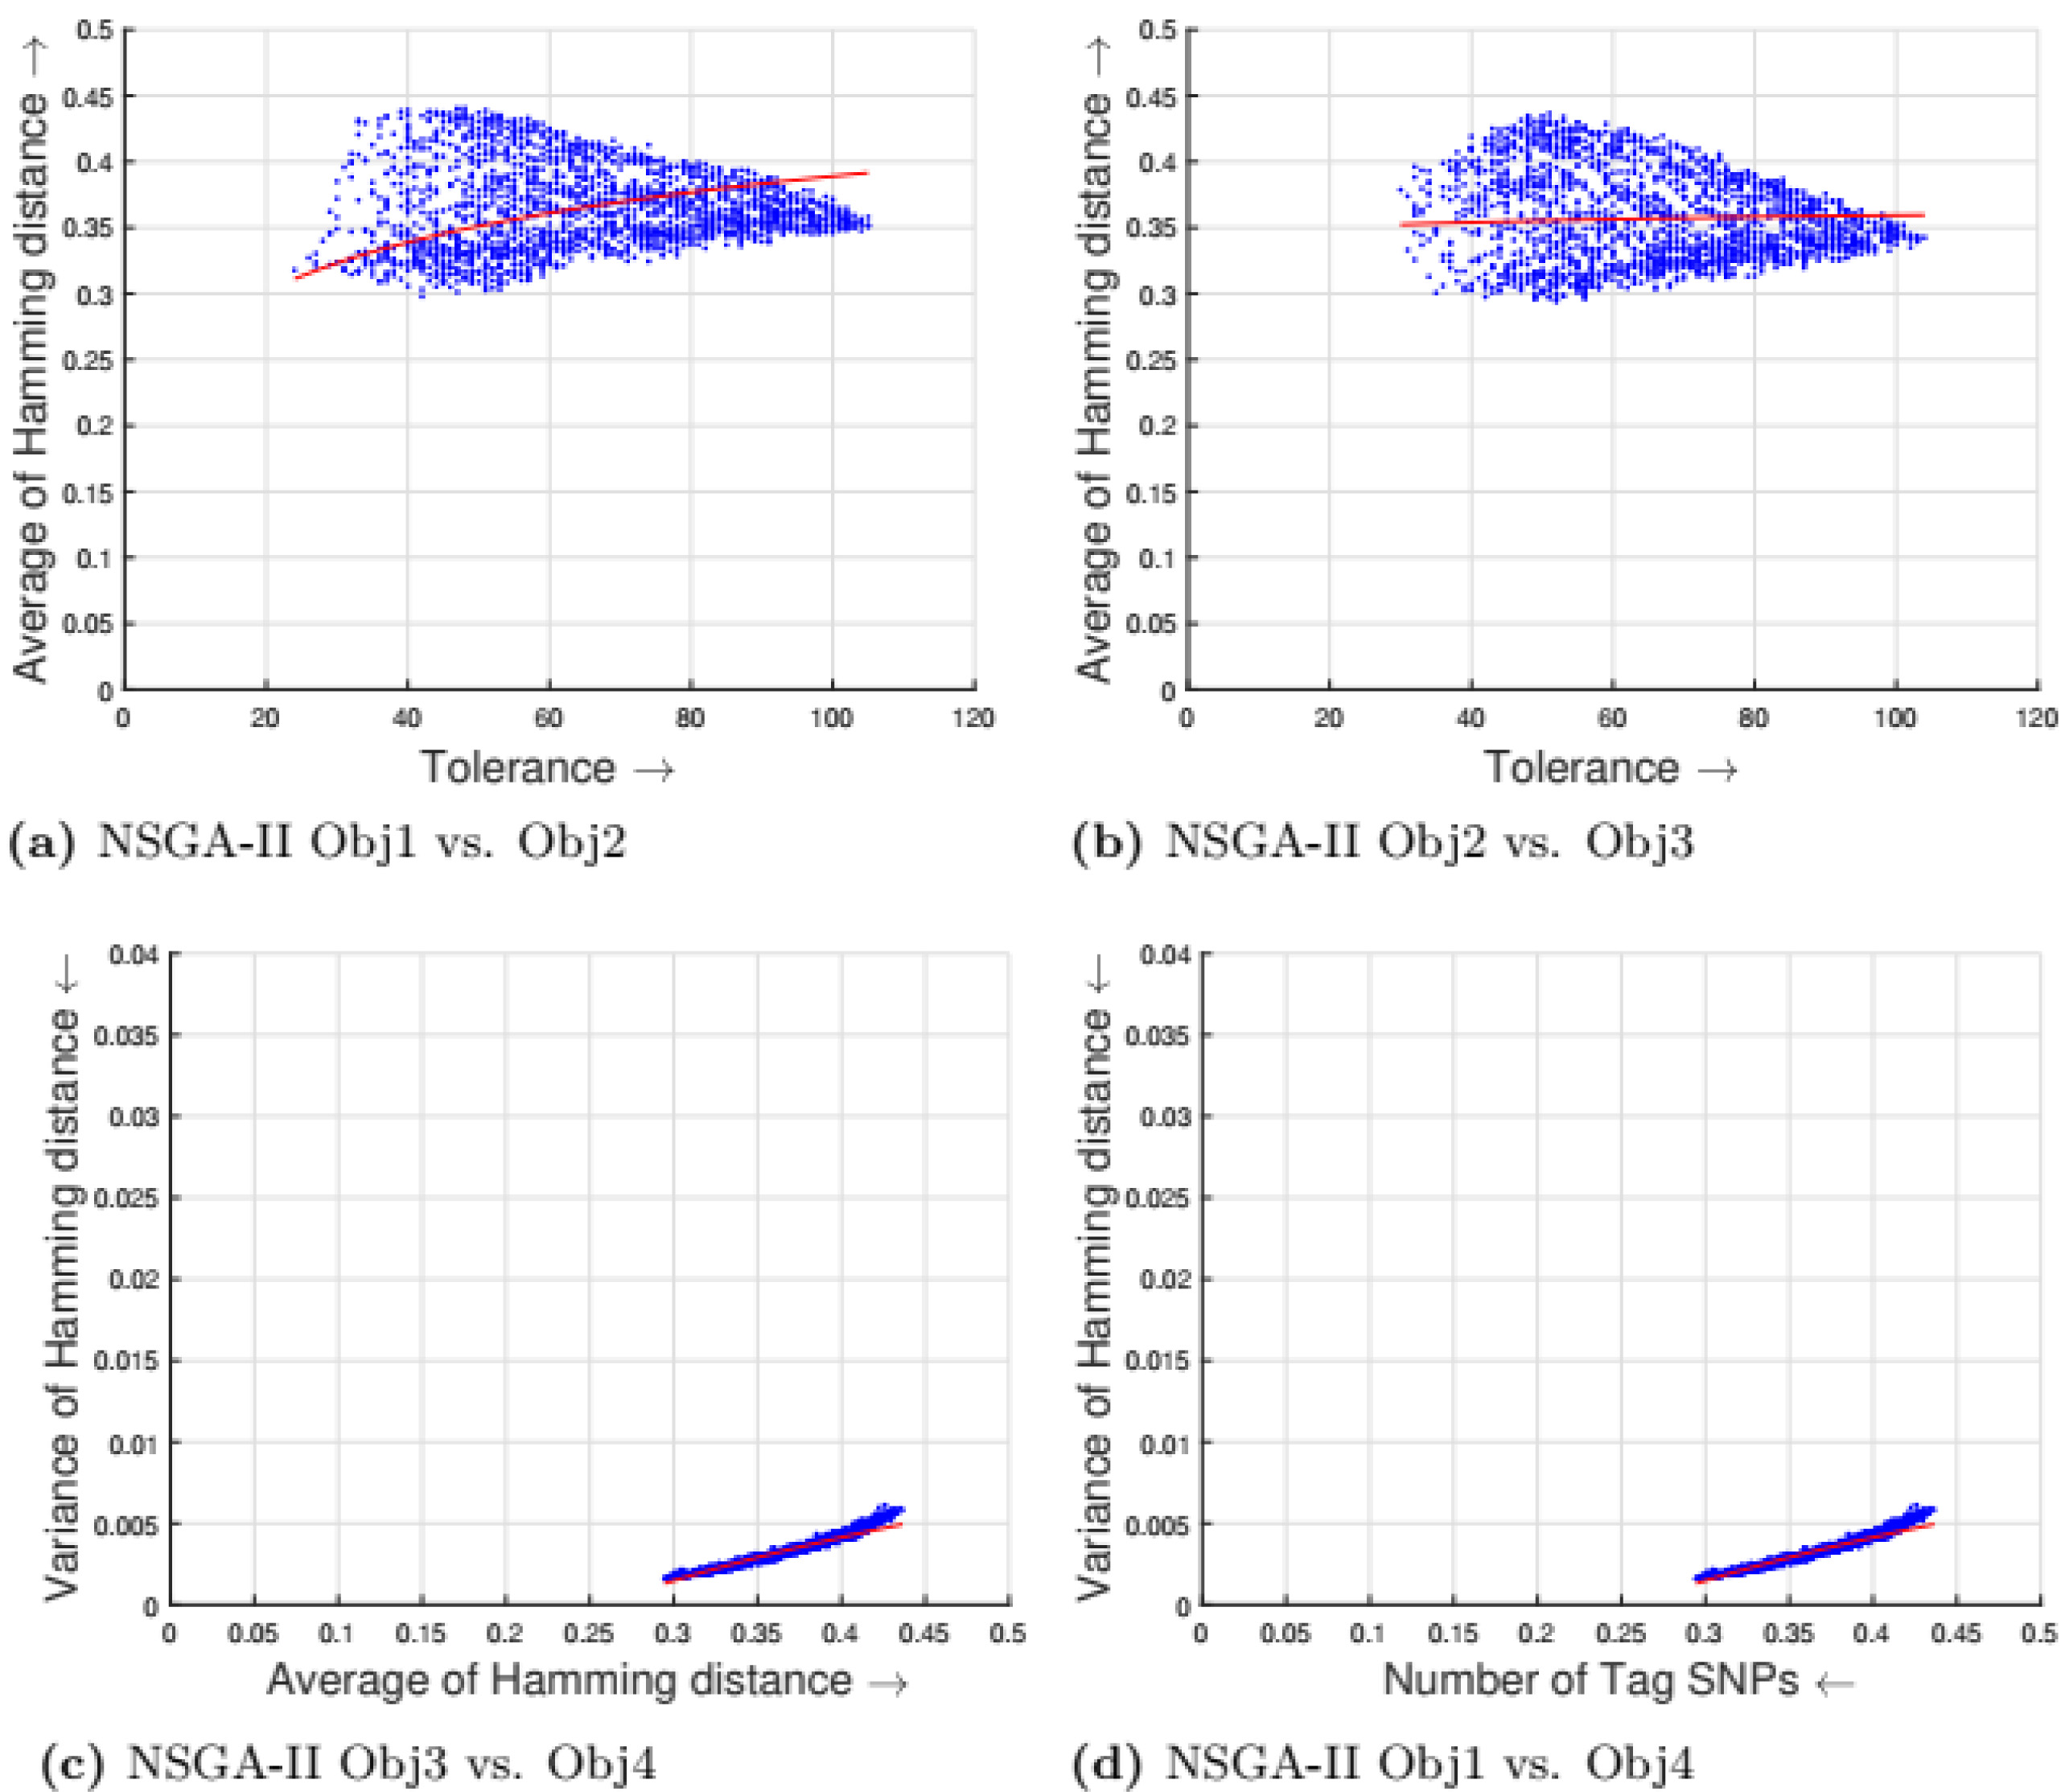
\includegraphics[width=\textwidth]{analisis_assets/moqa_2022/figures/moqa_fig_nsga2_random.jpeg}
        \caption{NSGA-II (RI)}
    \end{subfigure}
    \hfill
    \begin{subfigure}[b]{0.45\textwidth}
        \centering
        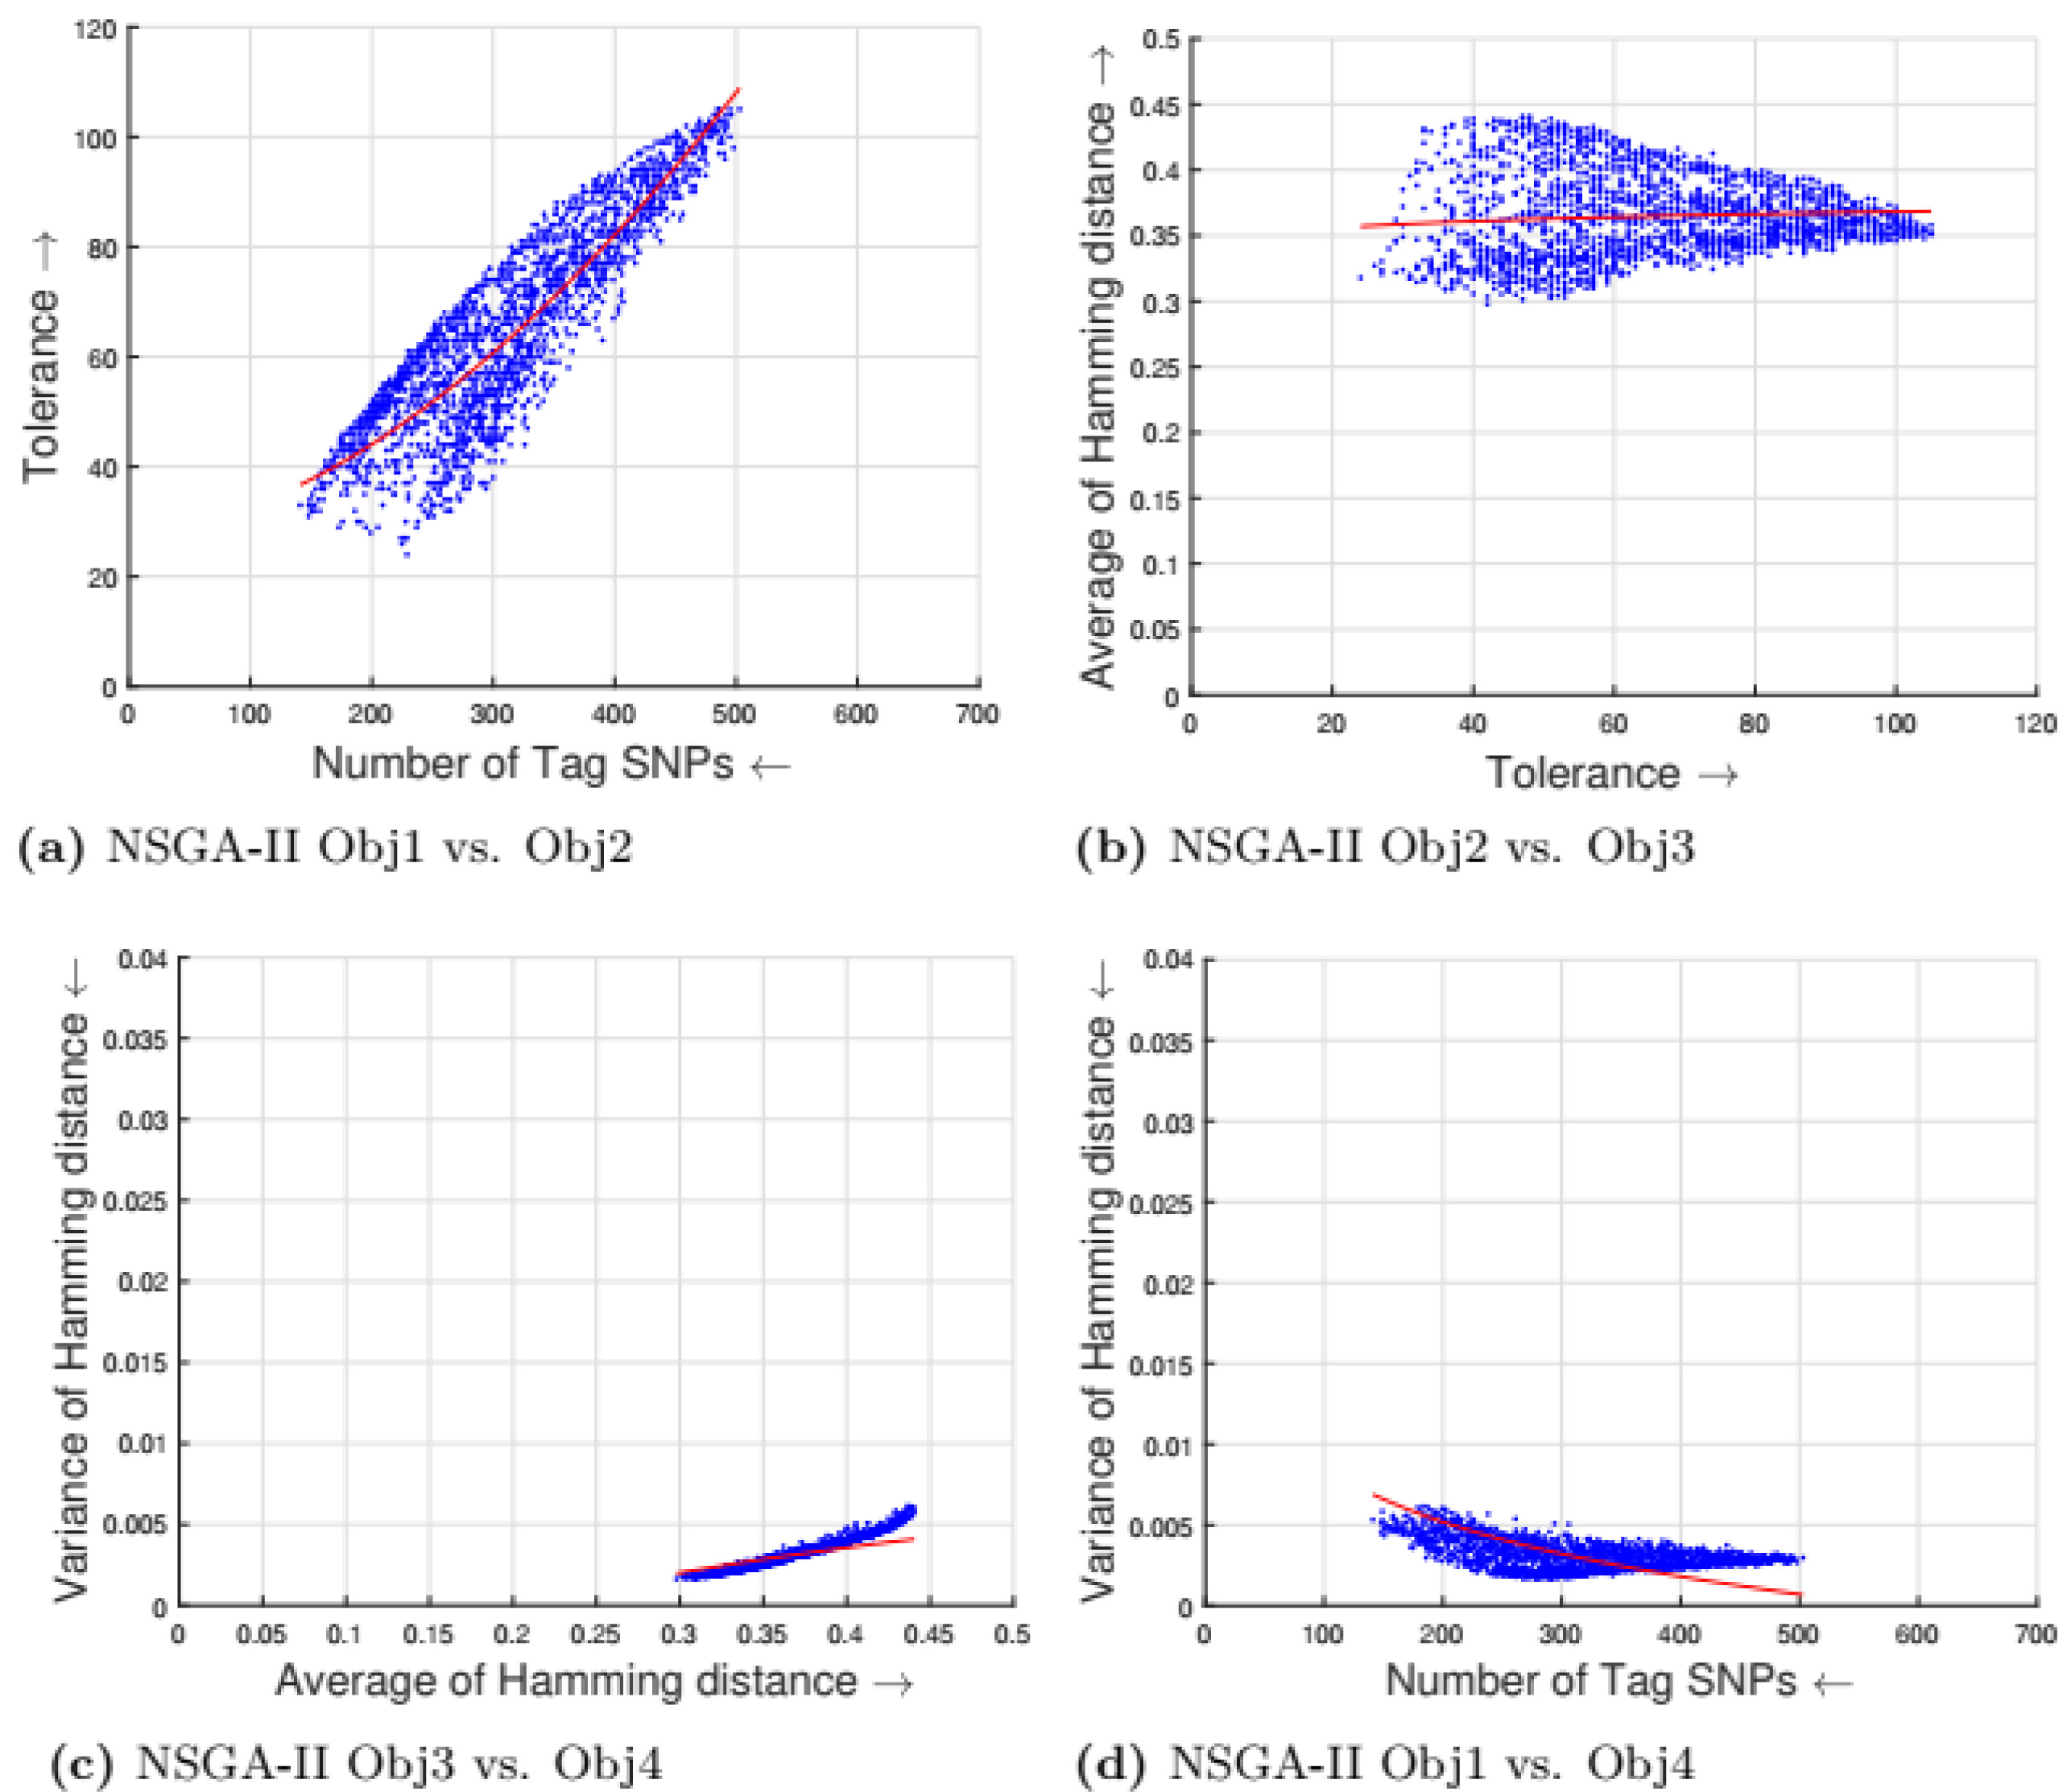
\includegraphics[width=\textwidth]{analisis_assets/moqa_2022/figures/moqa_fig_nsga2_greedy.jpeg}
        \caption{NSGA-II (GI)}
    \end{subfigure}
    \vskip\baselineskip
    \begin{subfigure}[b]{0.45\textwidth}
        \centering
        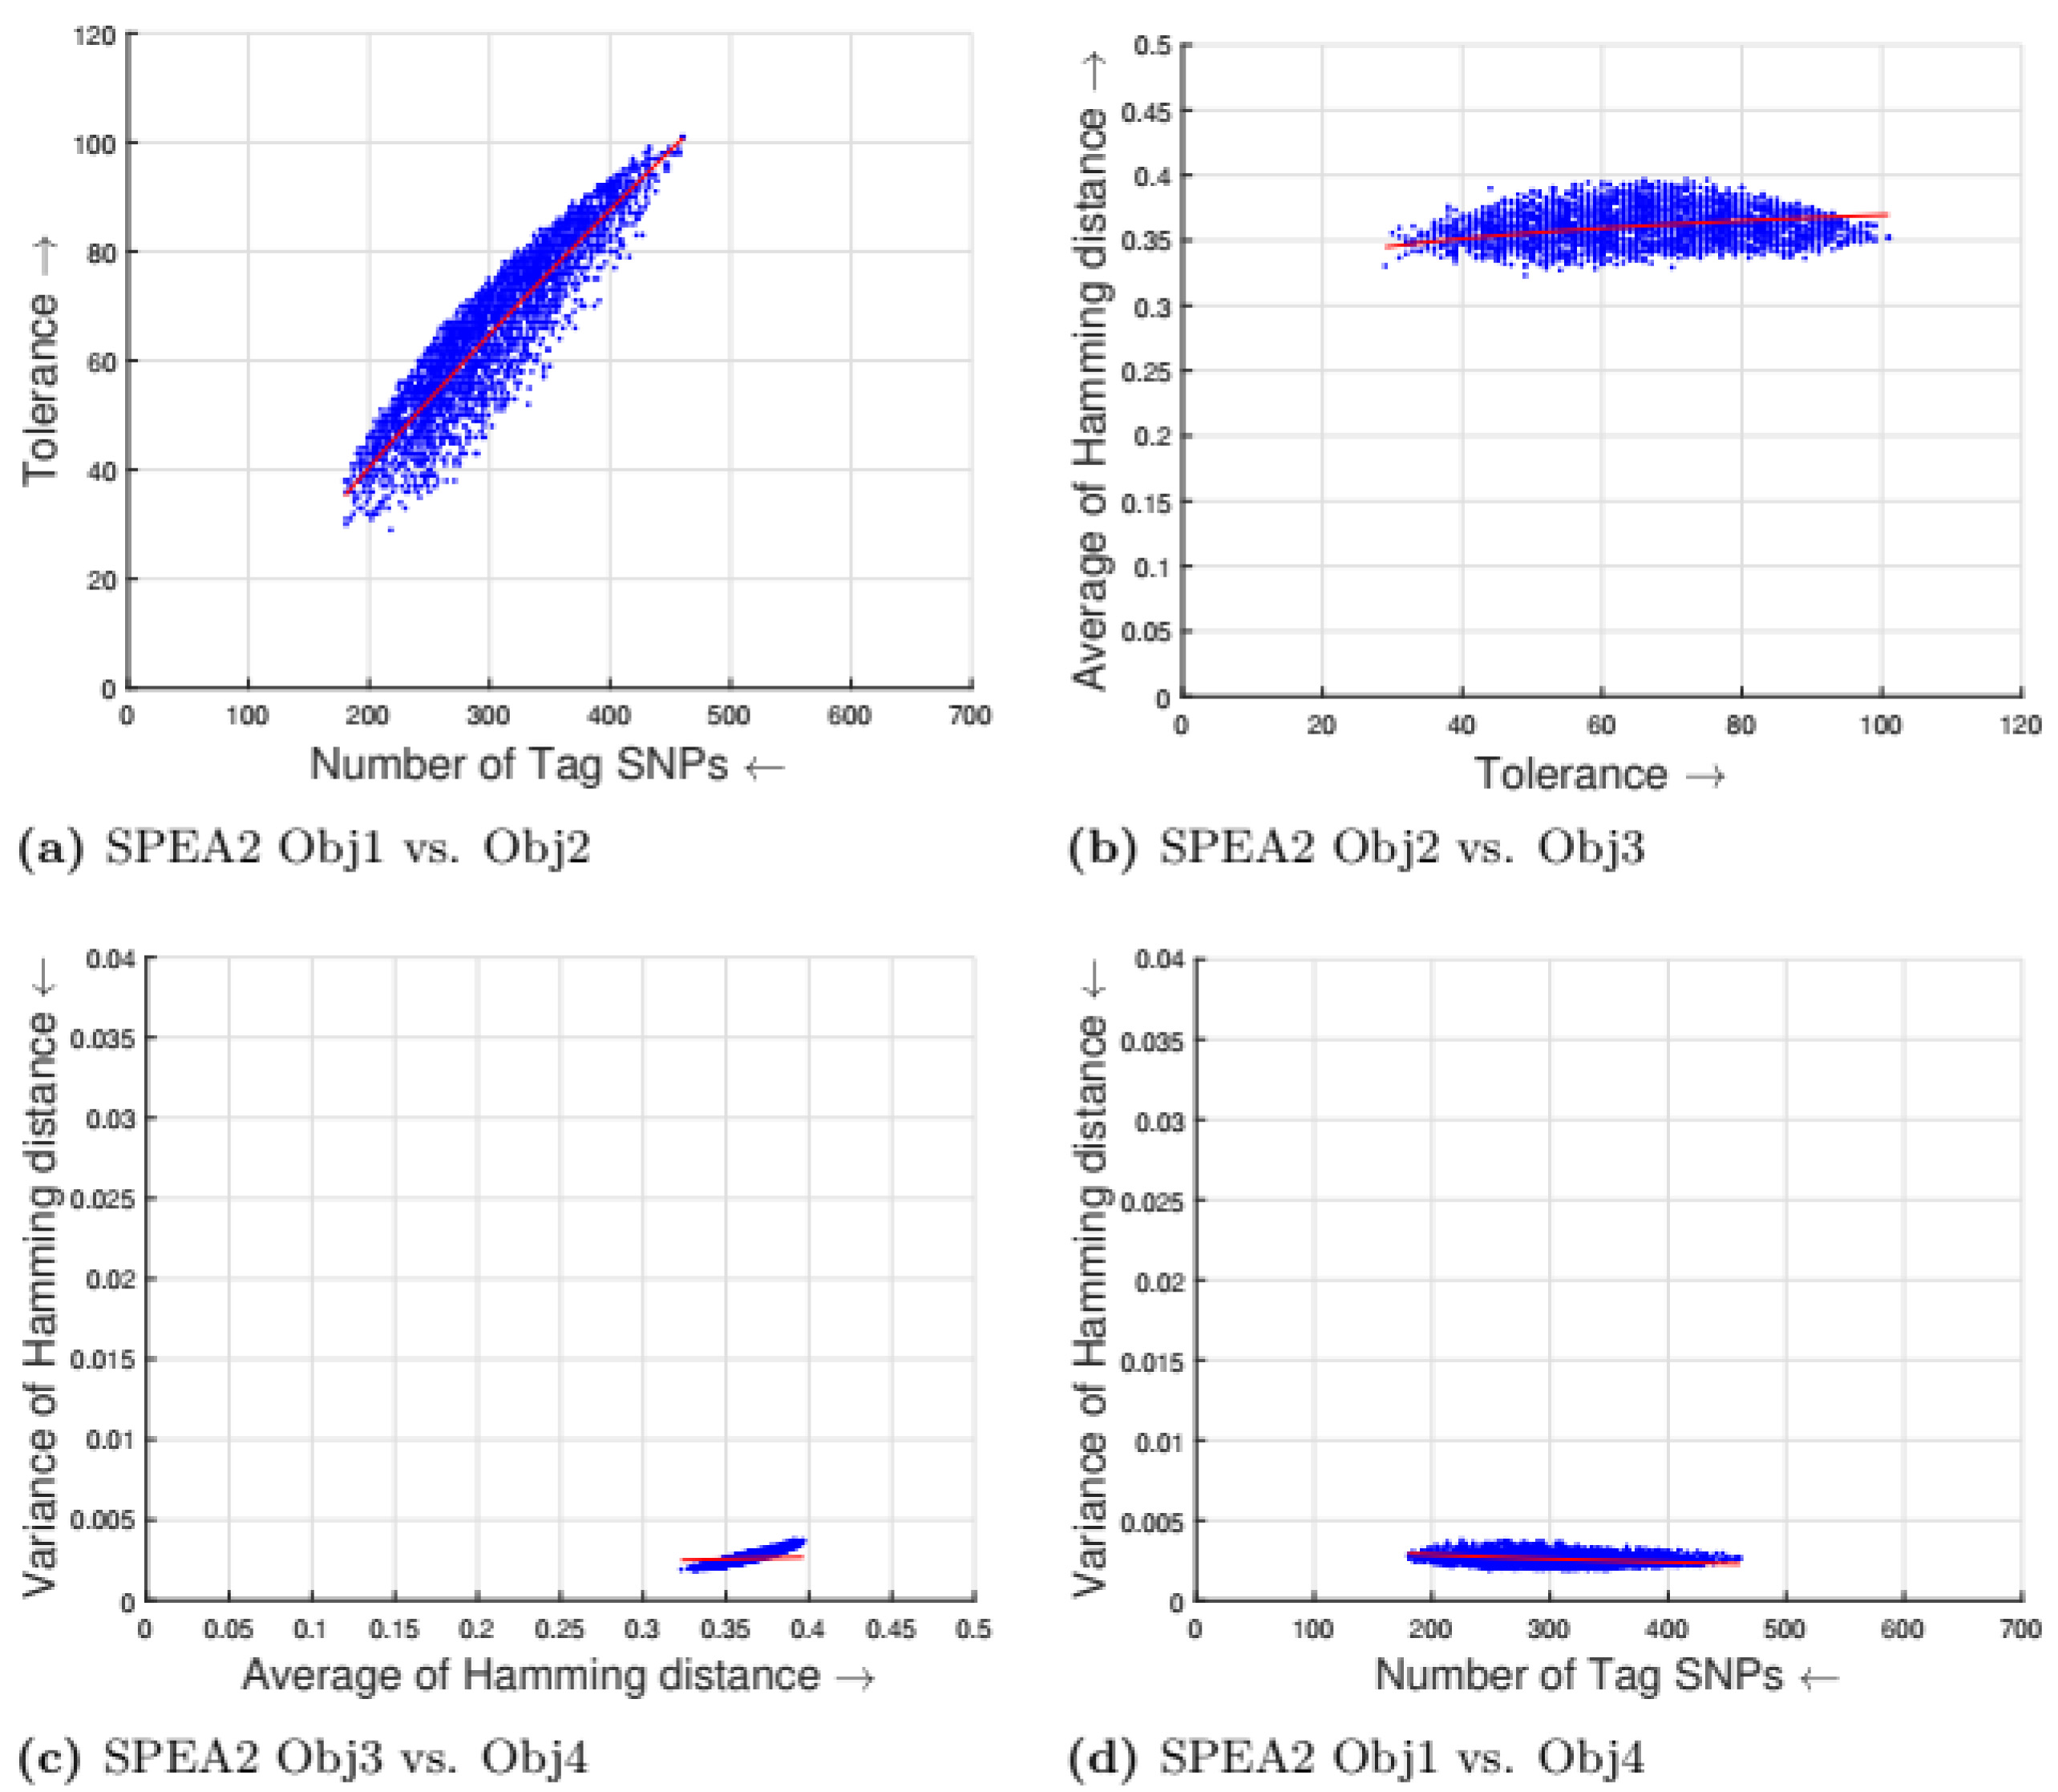
\includegraphics[width=\textwidth]{analisis_assets/moqa_2022/figures/moqa_fig_spea2_random.jpeg}
        \caption{SPEA2 (RI)}
    \end{subfigure}
    \hfill
    \begin{subfigure}[b]{0.45\textwidth}
        \centering
        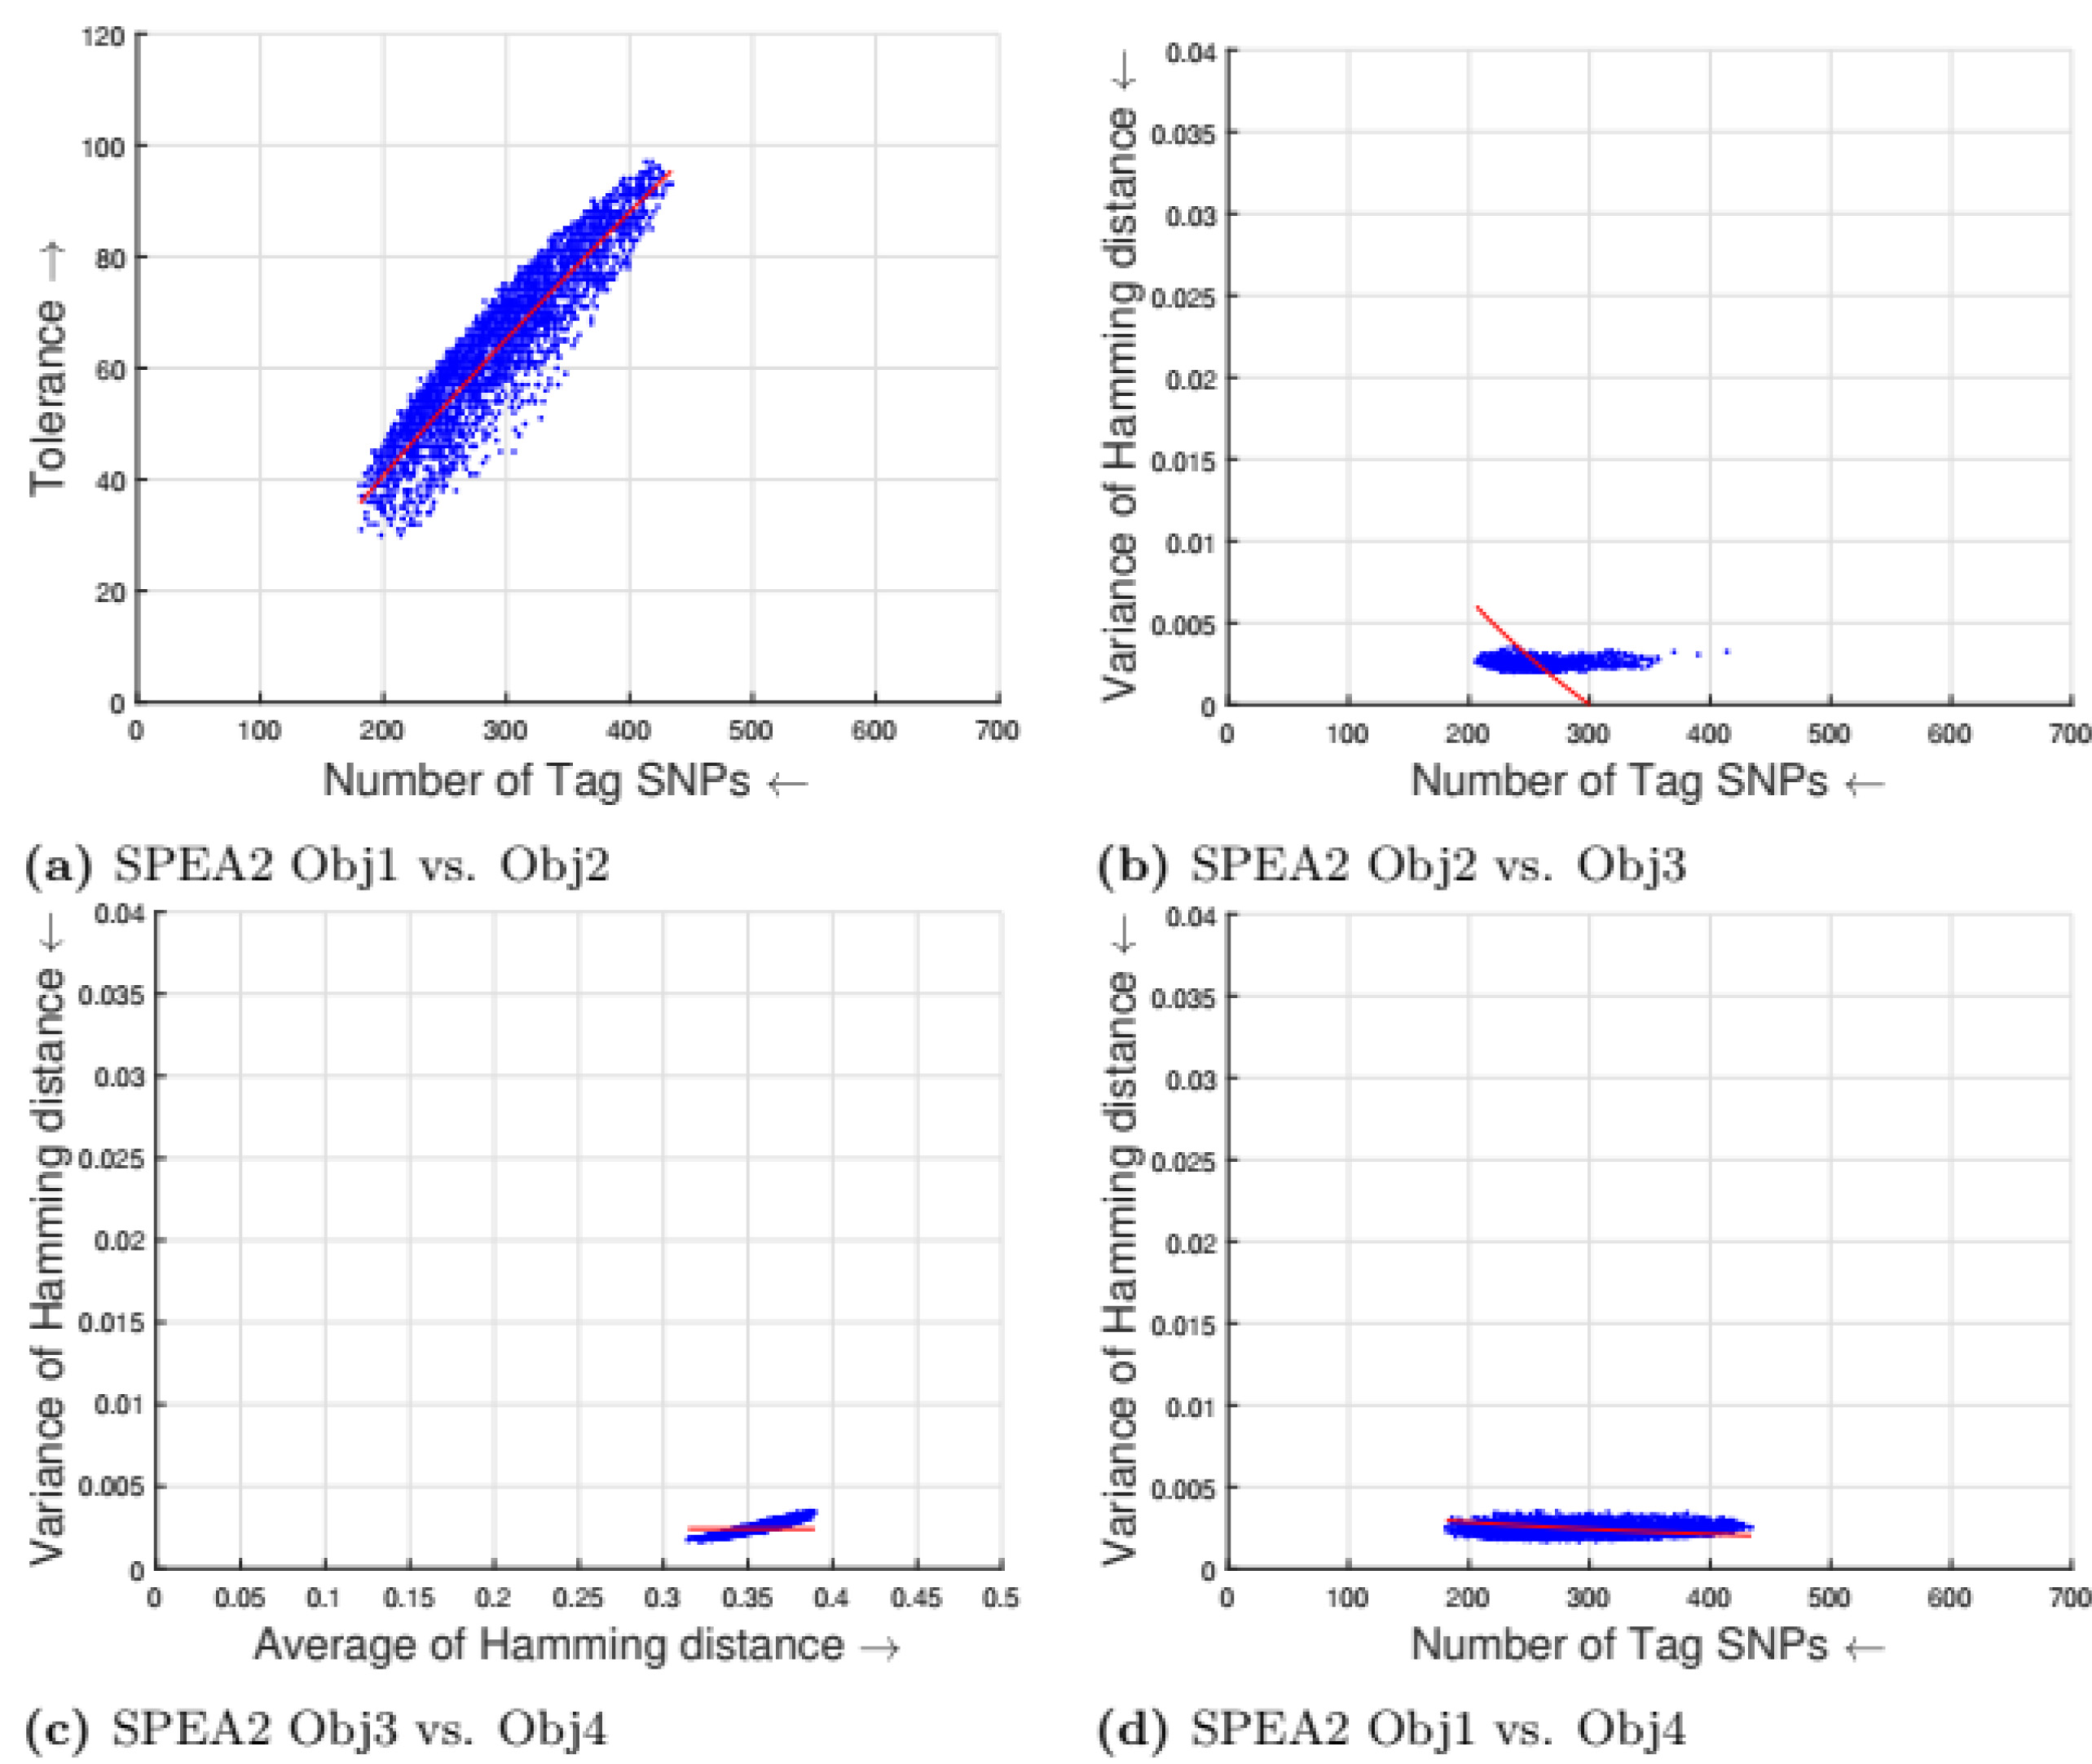
\includegraphics[width=\textwidth]{analisis_assets/moqa_2022/figures/moqa_fig_spea2_greedy.jpeg}
        \caption{SPEA2 (GI)}
    \end{subfigure}
    \caption{Comparativa de Frentes de Pareto: NSGA-II y SPEA2 (Moqa 2022).}
\end{figure}

\begin{figure}[H]
    \centering
    \begin{subfigure}[b]{0.45\textwidth}
        \centering
        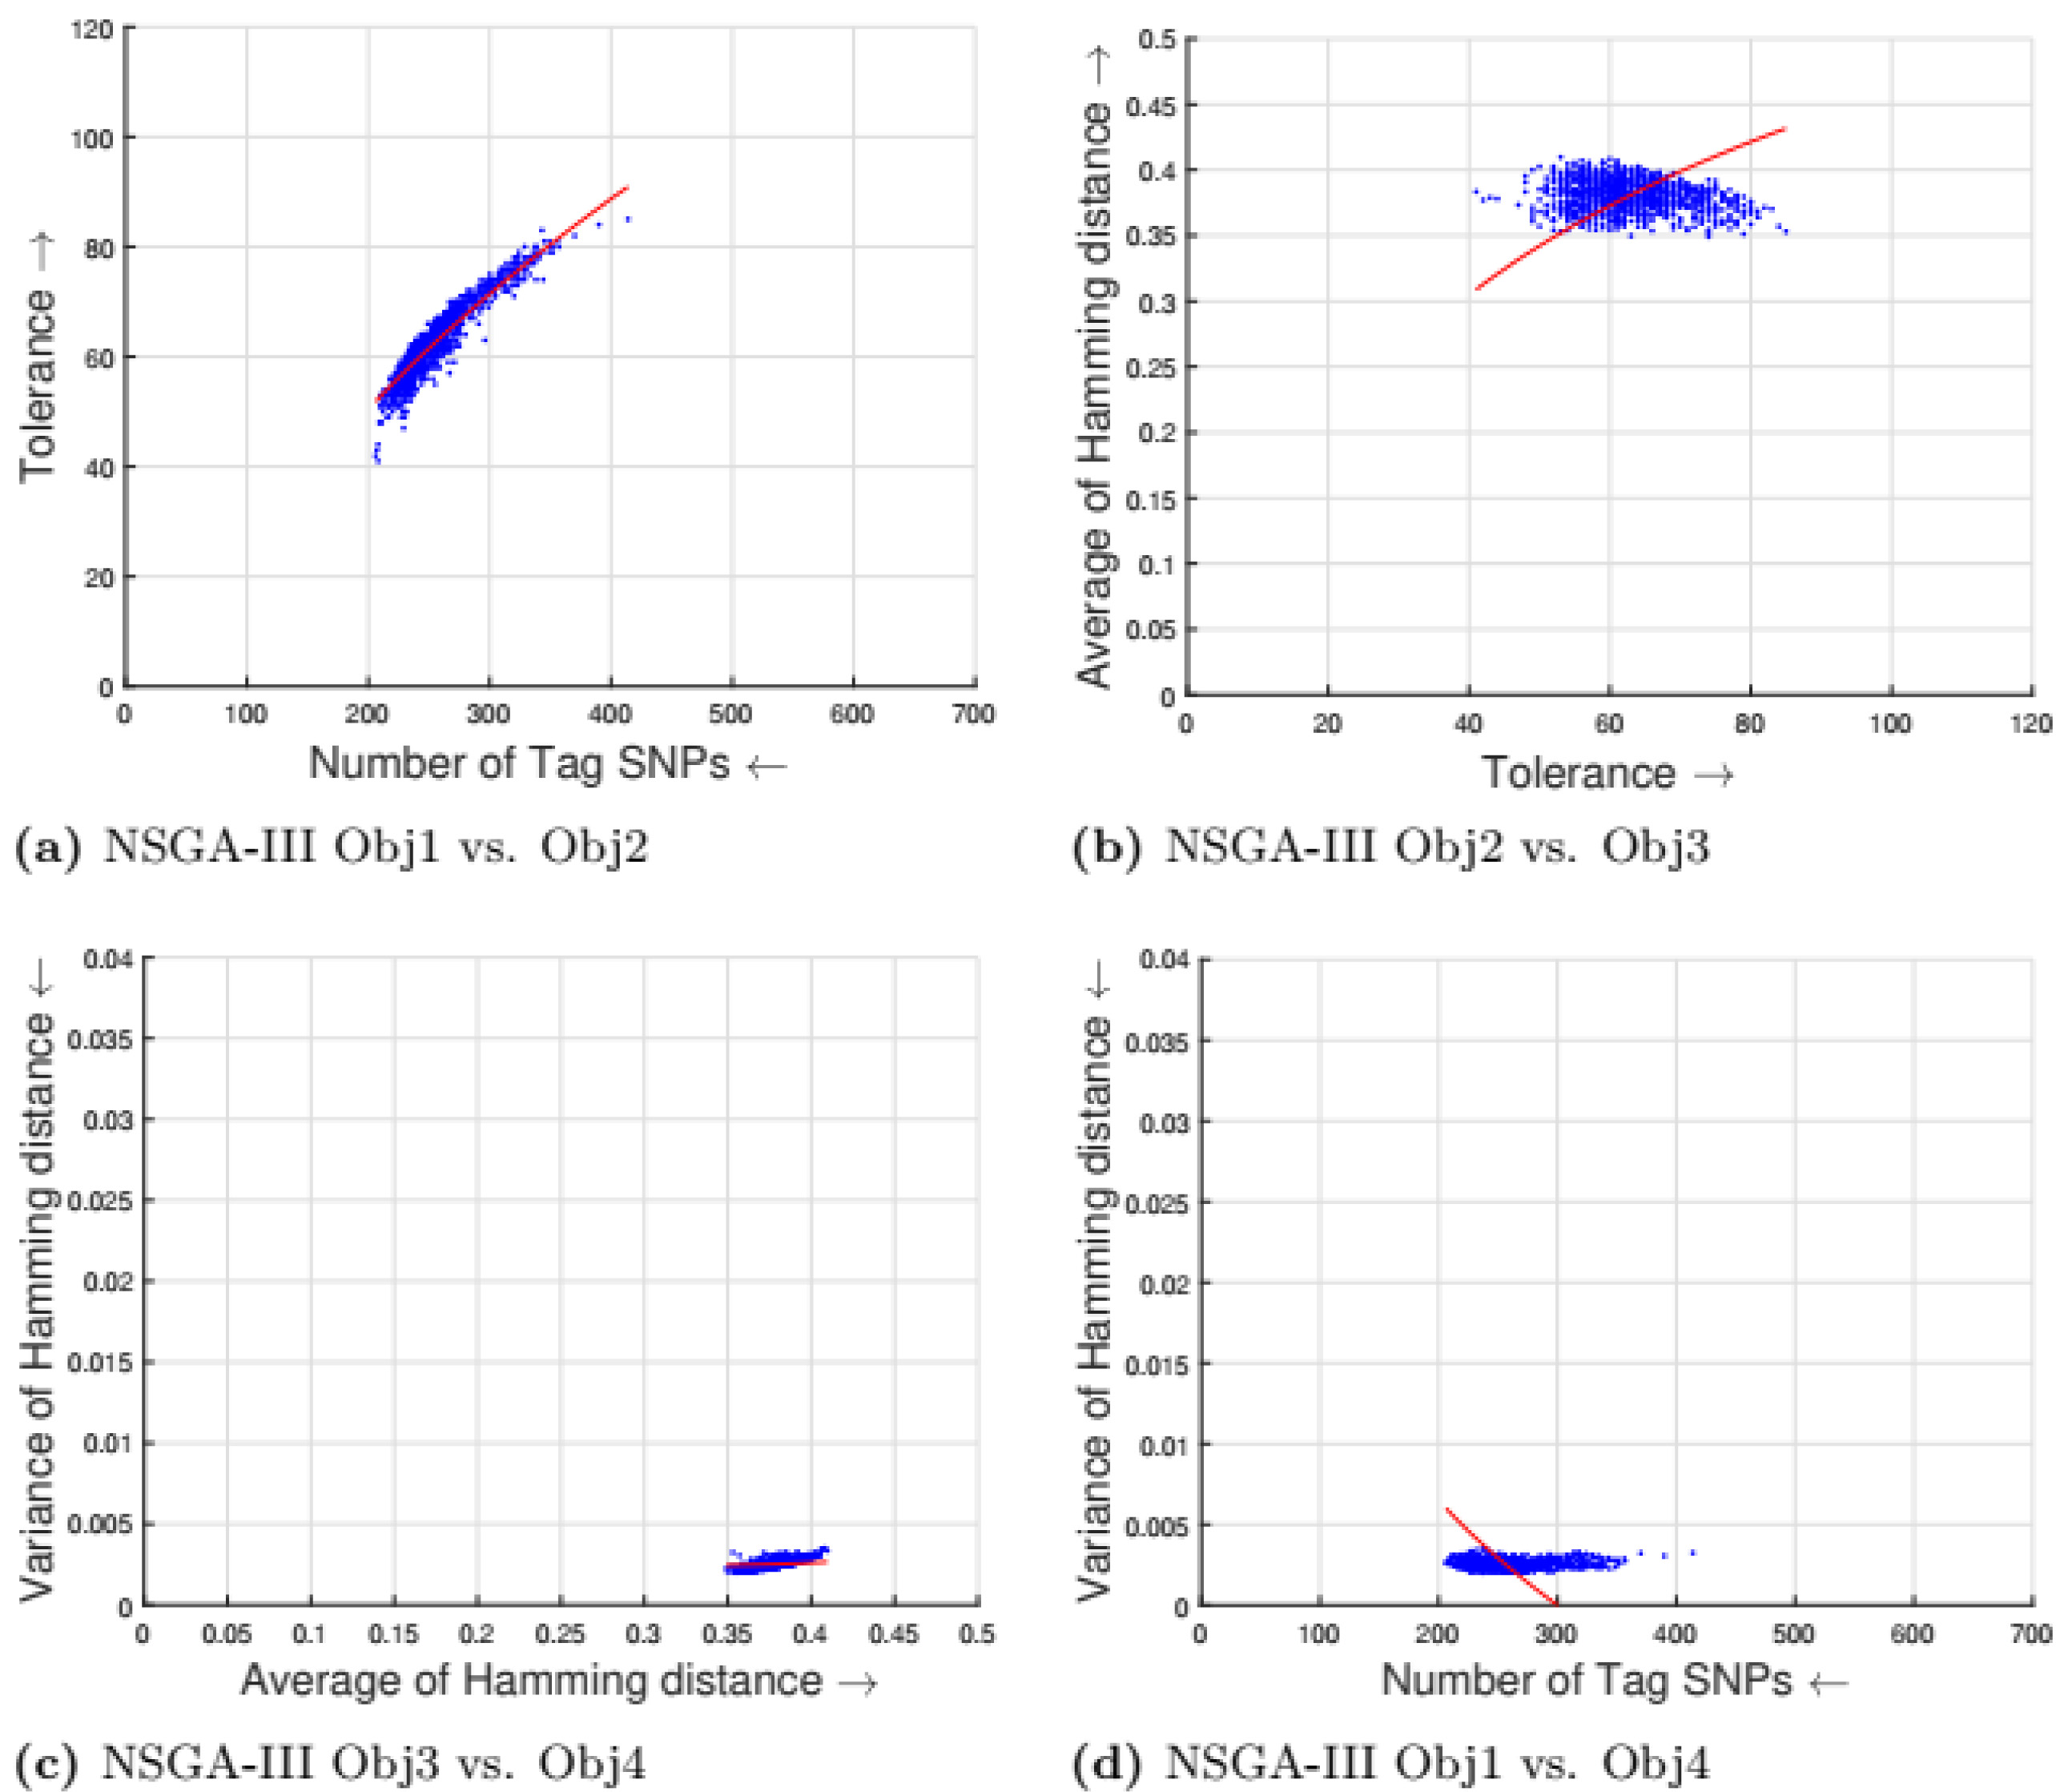
\includegraphics[width=\textwidth]{analisis_assets/moqa_2022/figures/moqa_fig_nsga3_random.jpeg}
        \caption{NSGA-III (RI)}
    \end{subfigure}
    \hfill
    \begin{subfigure}[b]{0.45\textwidth}
        \centering
        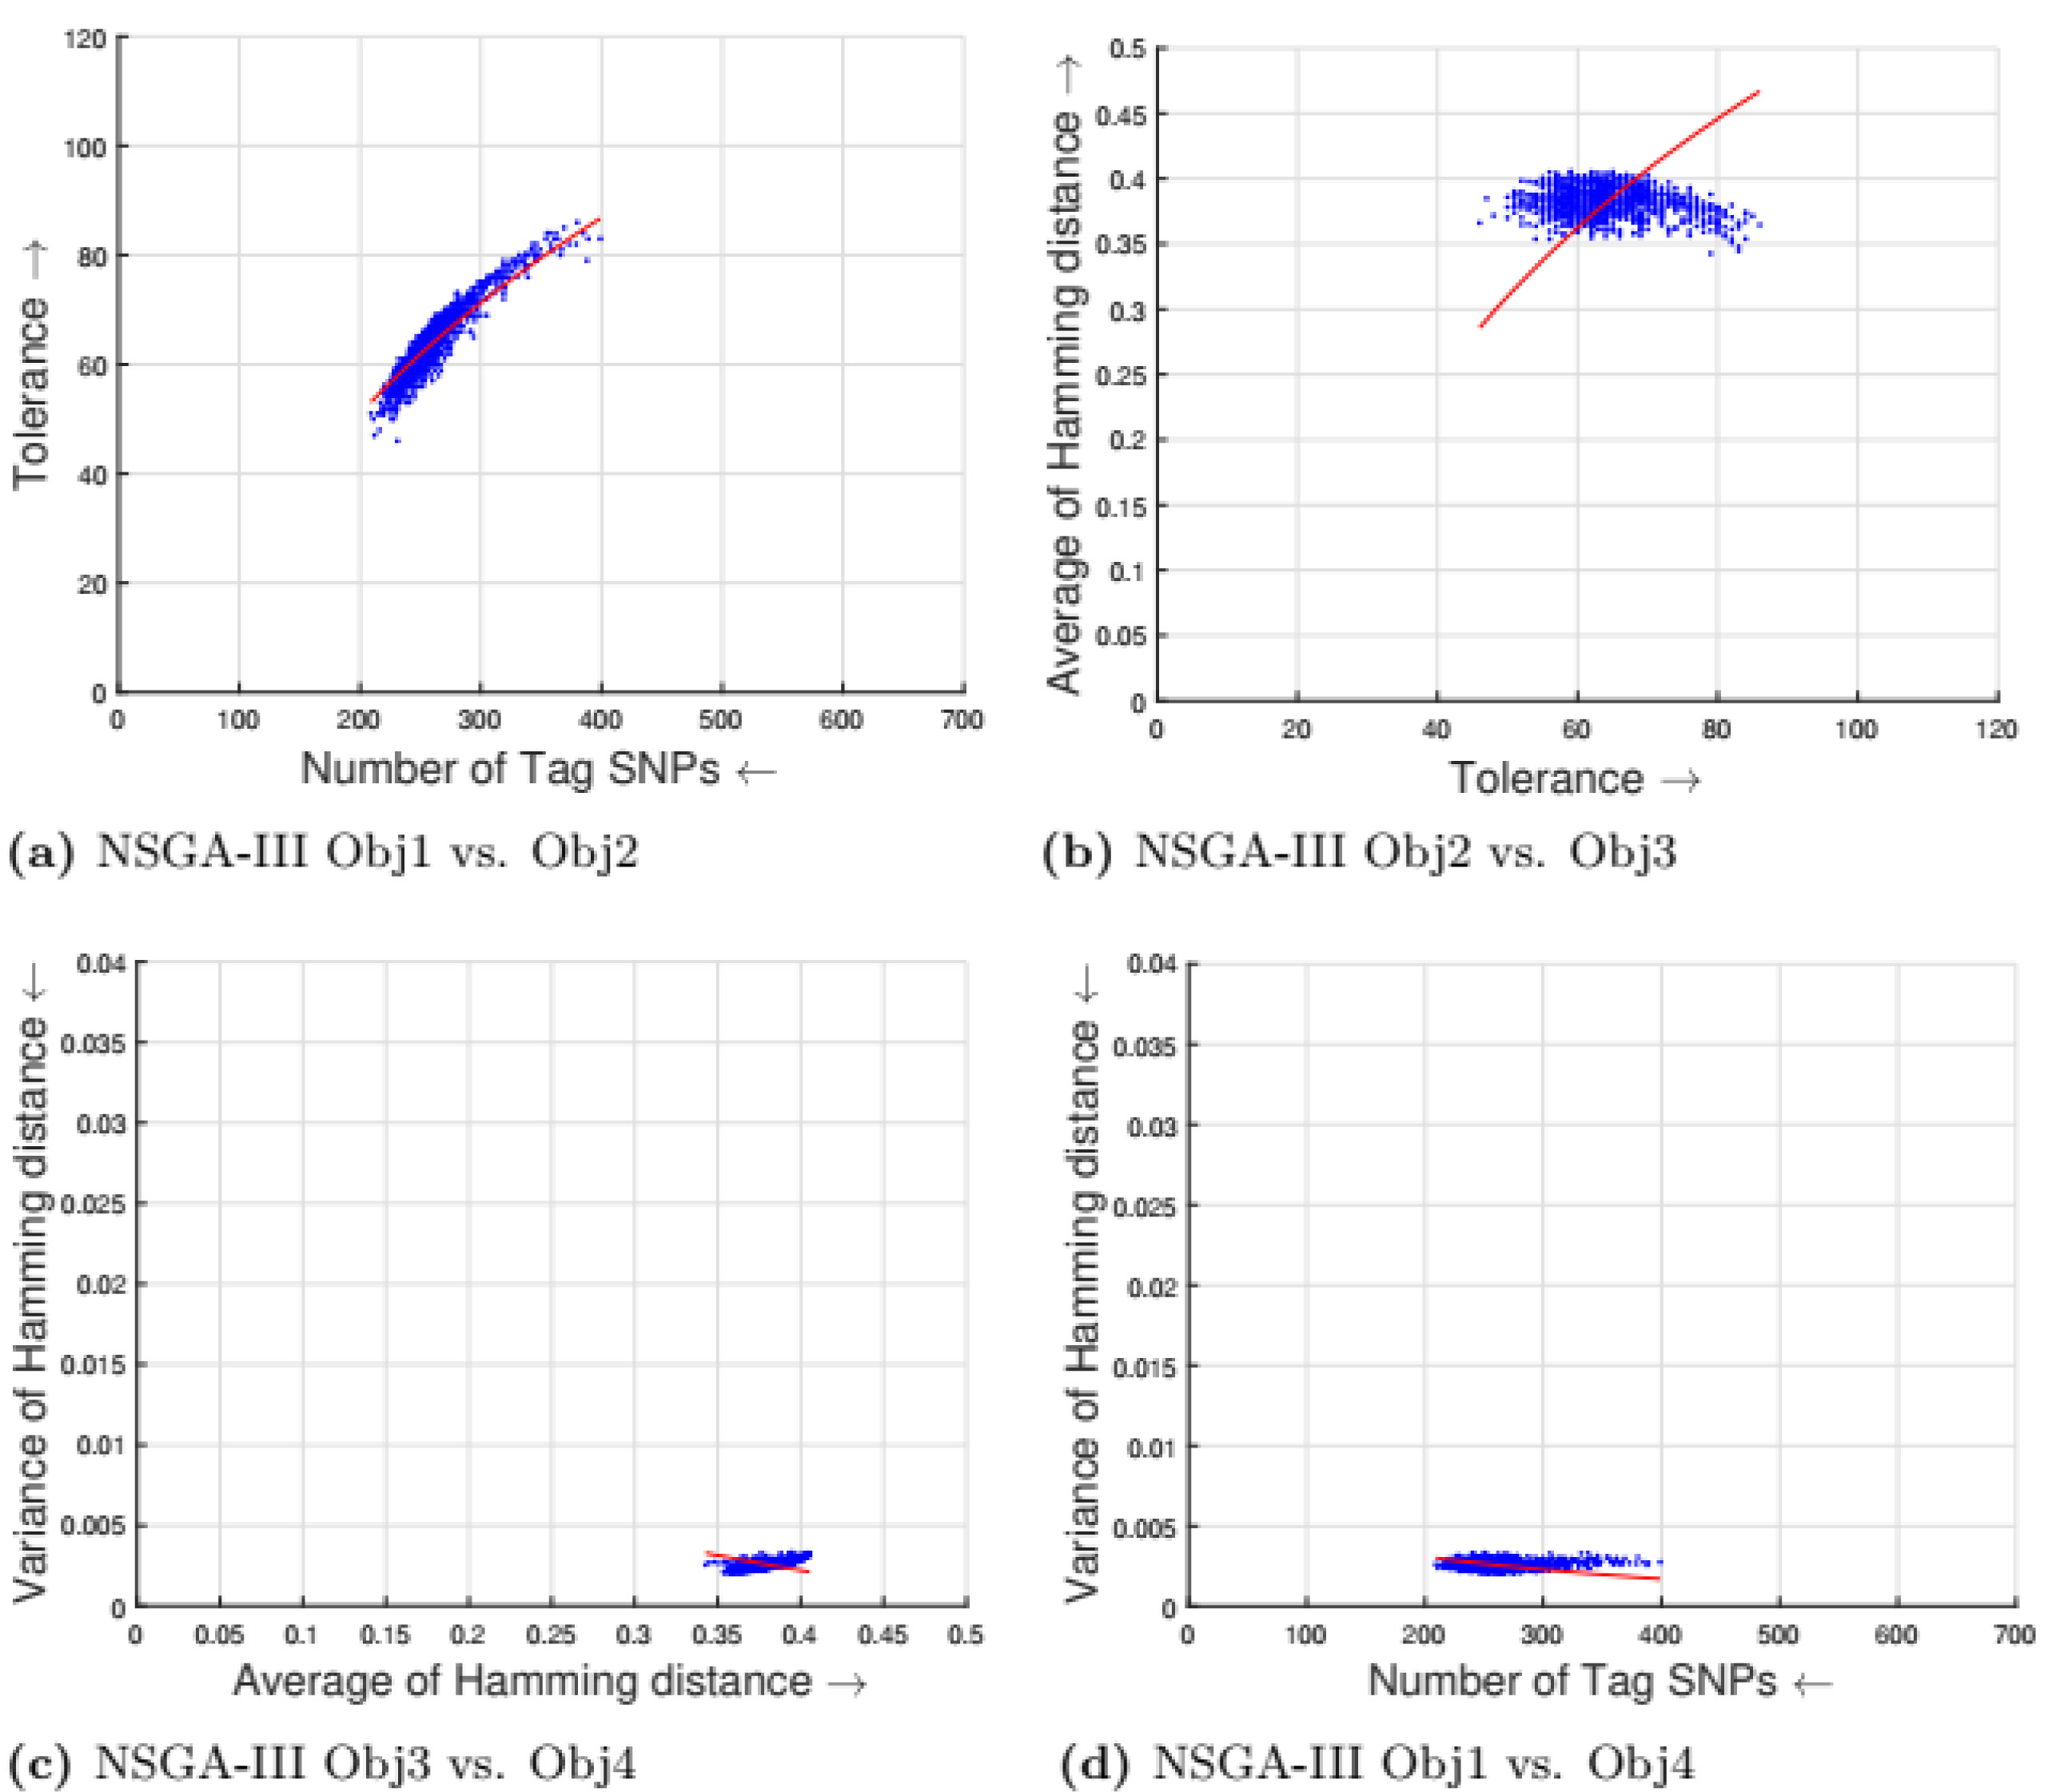
\includegraphics[width=\textwidth]{analisis_assets/moqa_2022/figures/moqa_fig_nsga3_greedy.jpeg}
        \caption{NSGA-III (GI)}
    \end{subfigure}
    \vskip\baselineskip
    \begin{subfigure}[b]{0.45\textwidth}
        \centering
        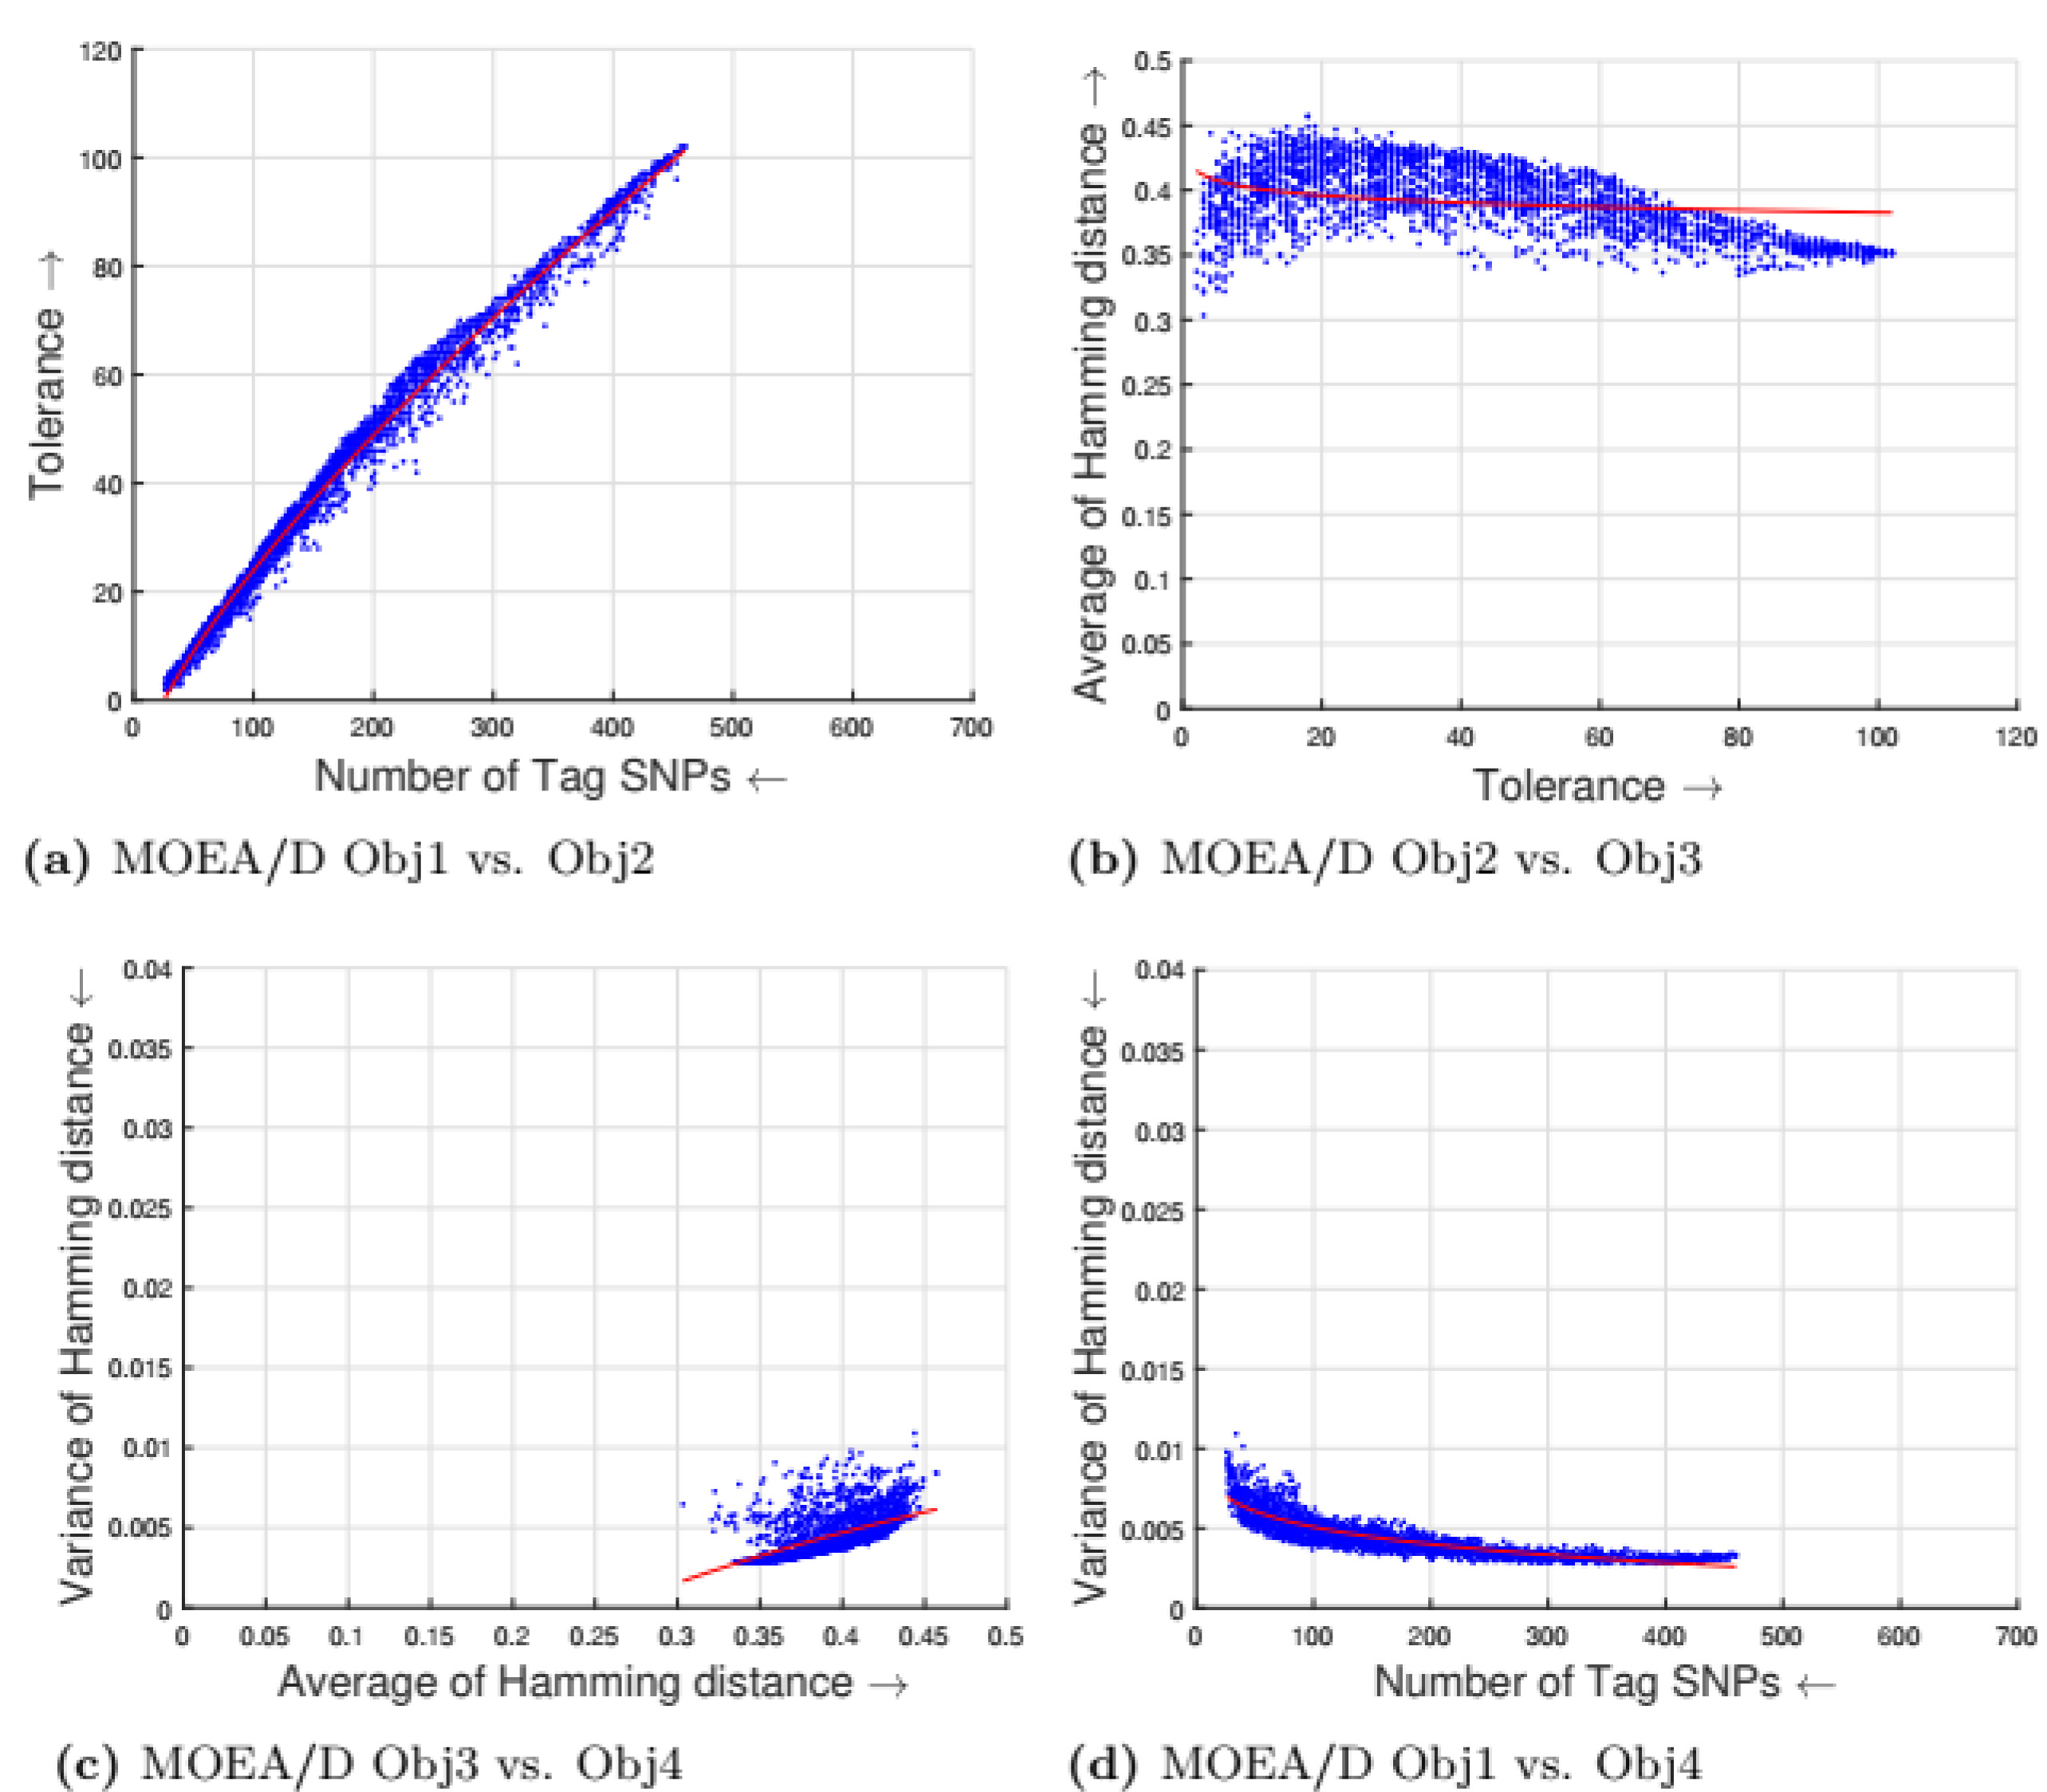
\includegraphics[width=\textwidth]{analisis_assets/moqa_2022/figures/moqa_fig_moead_random.jpeg}
        \caption{MOEA/D (RI)}
    \end{subfigure}
    \hfill
    \begin{subfigure}[b]{0.45\textwidth}
        \centering
        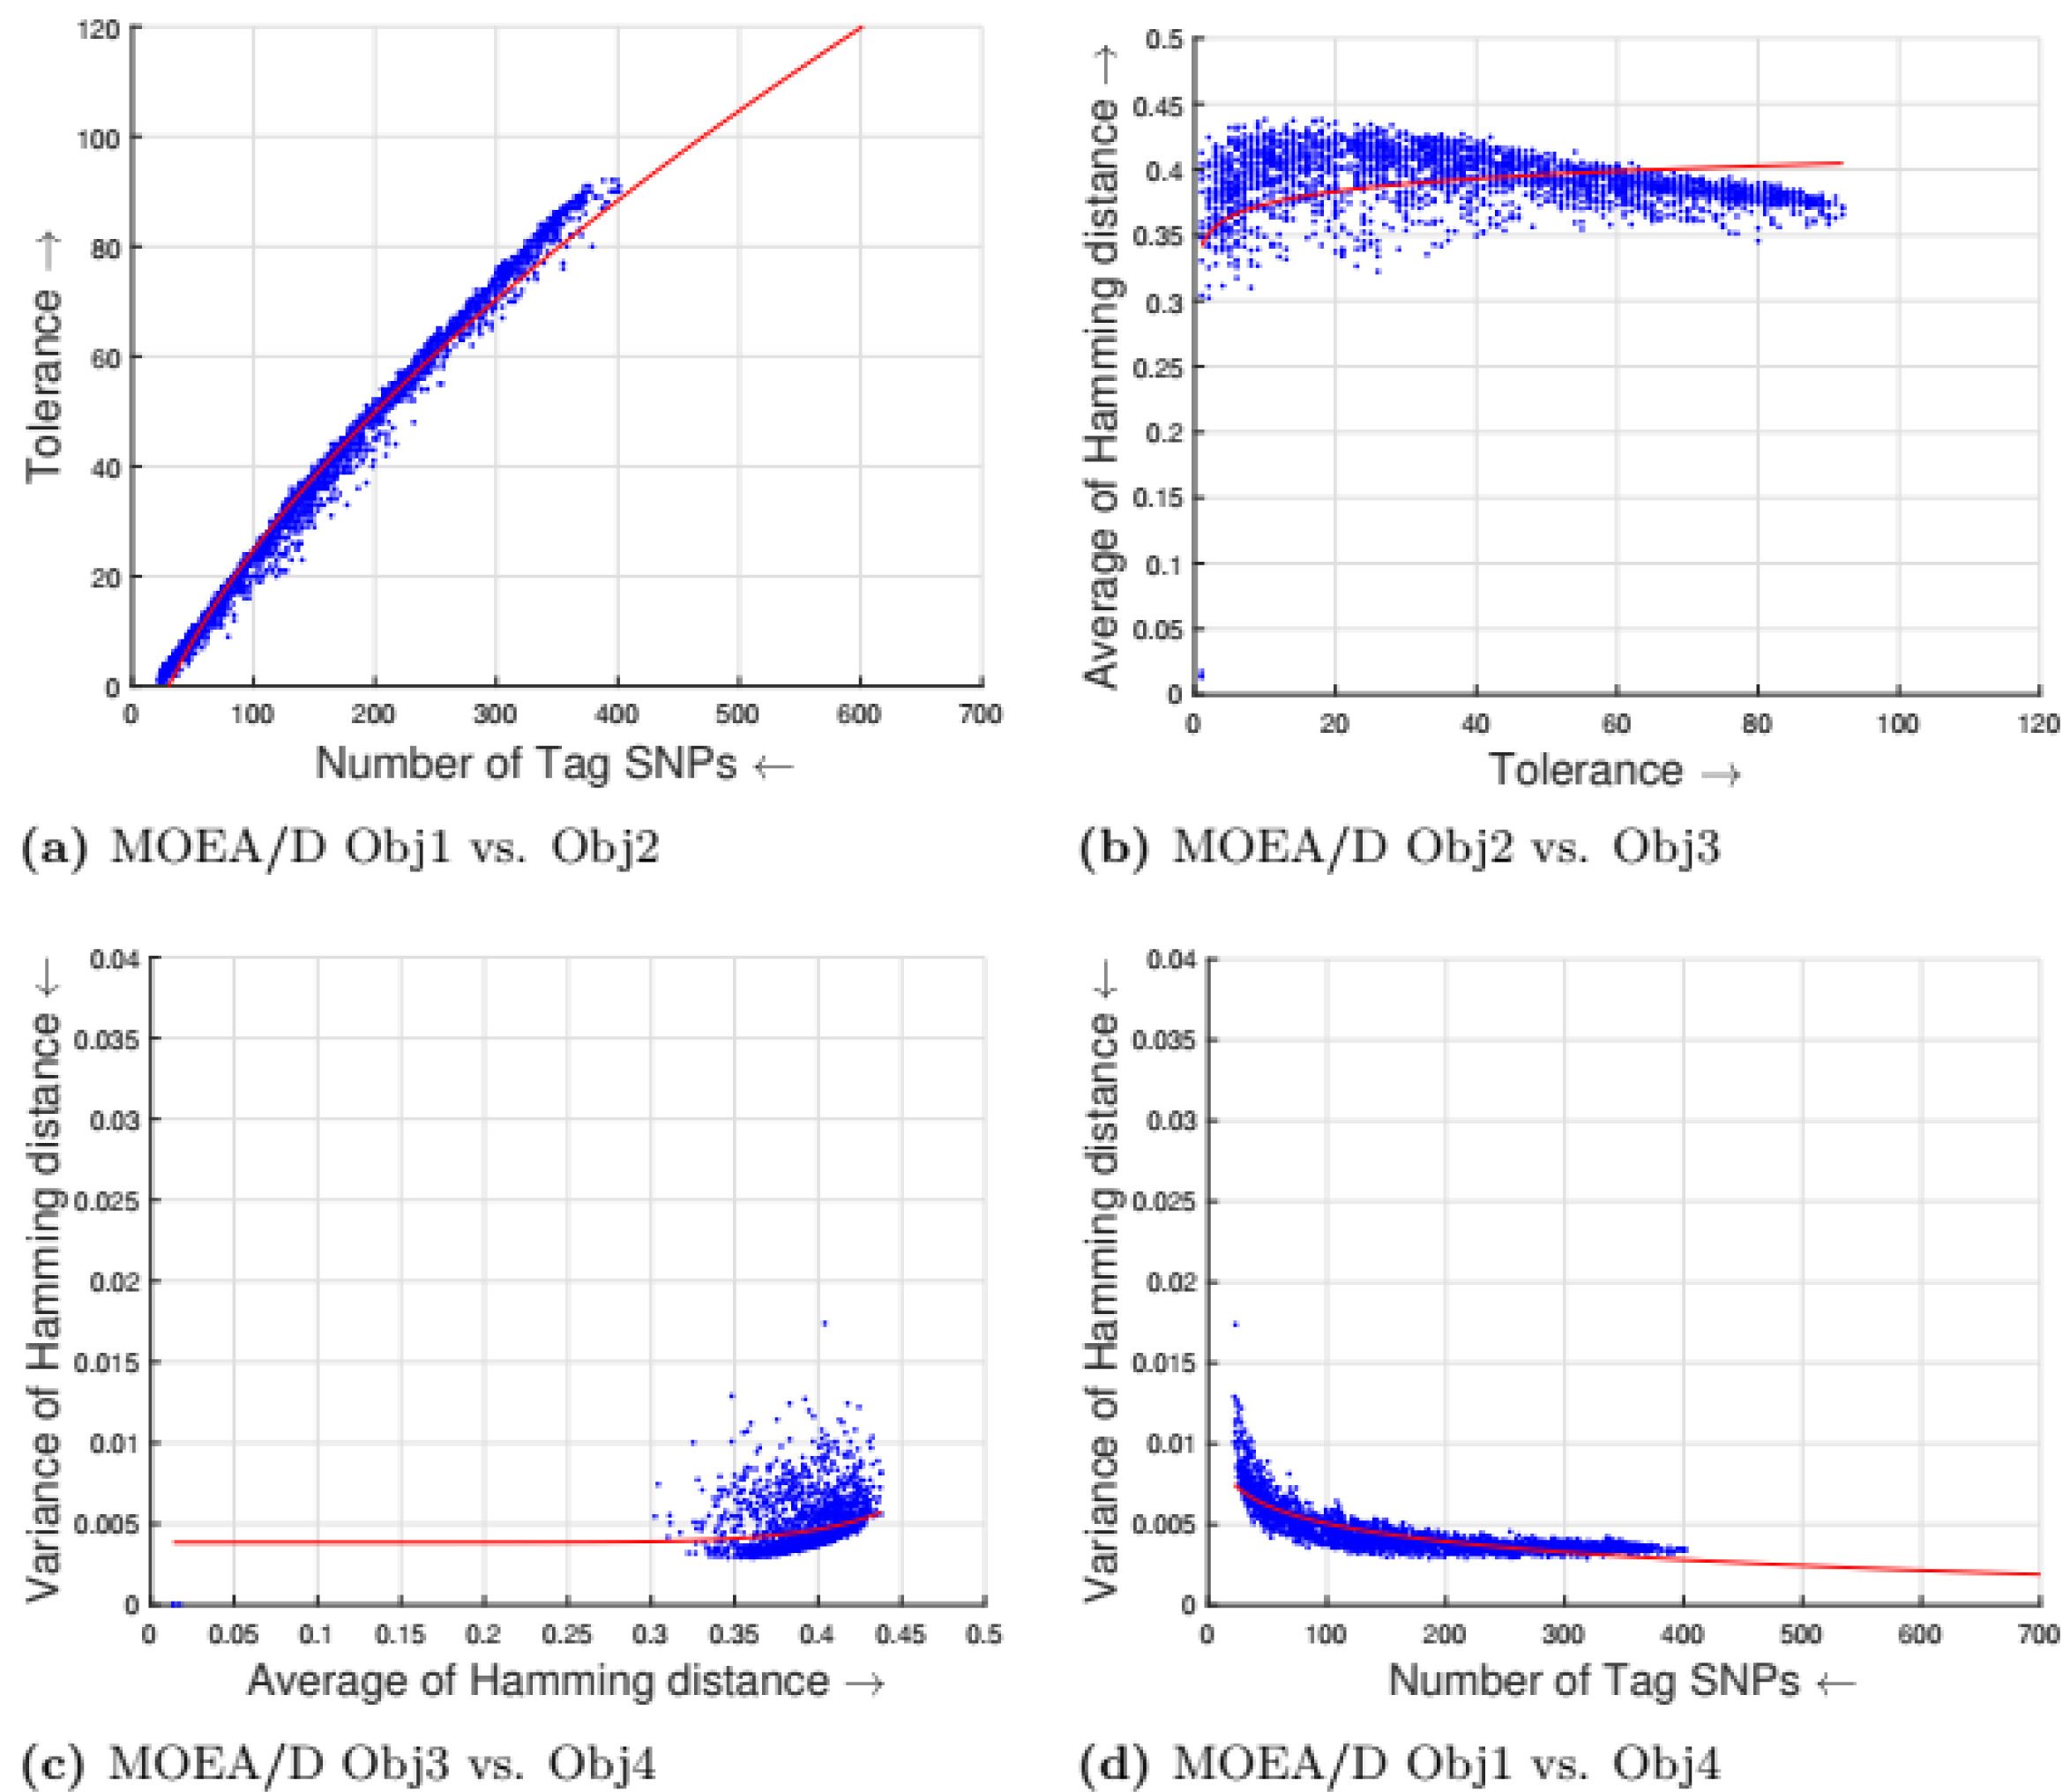
\includegraphics[width=\textwidth]{analisis_assets/moqa_2022/figures/moqa_fig_moead_greedy.jpeg}
        \caption{MOEA/D (GI)}
    \end{subfigure}
    \caption{Comparativa de Frentes de Pareto: NSGA-III y MOEA/D (Moqa 2022).}
\end{figure}

\subsubsection{Convergencia progresiva}
\begin{figure}[H]
    \centering
    \begin{subfigure}[b]{0.48\textwidth}
        \centering
        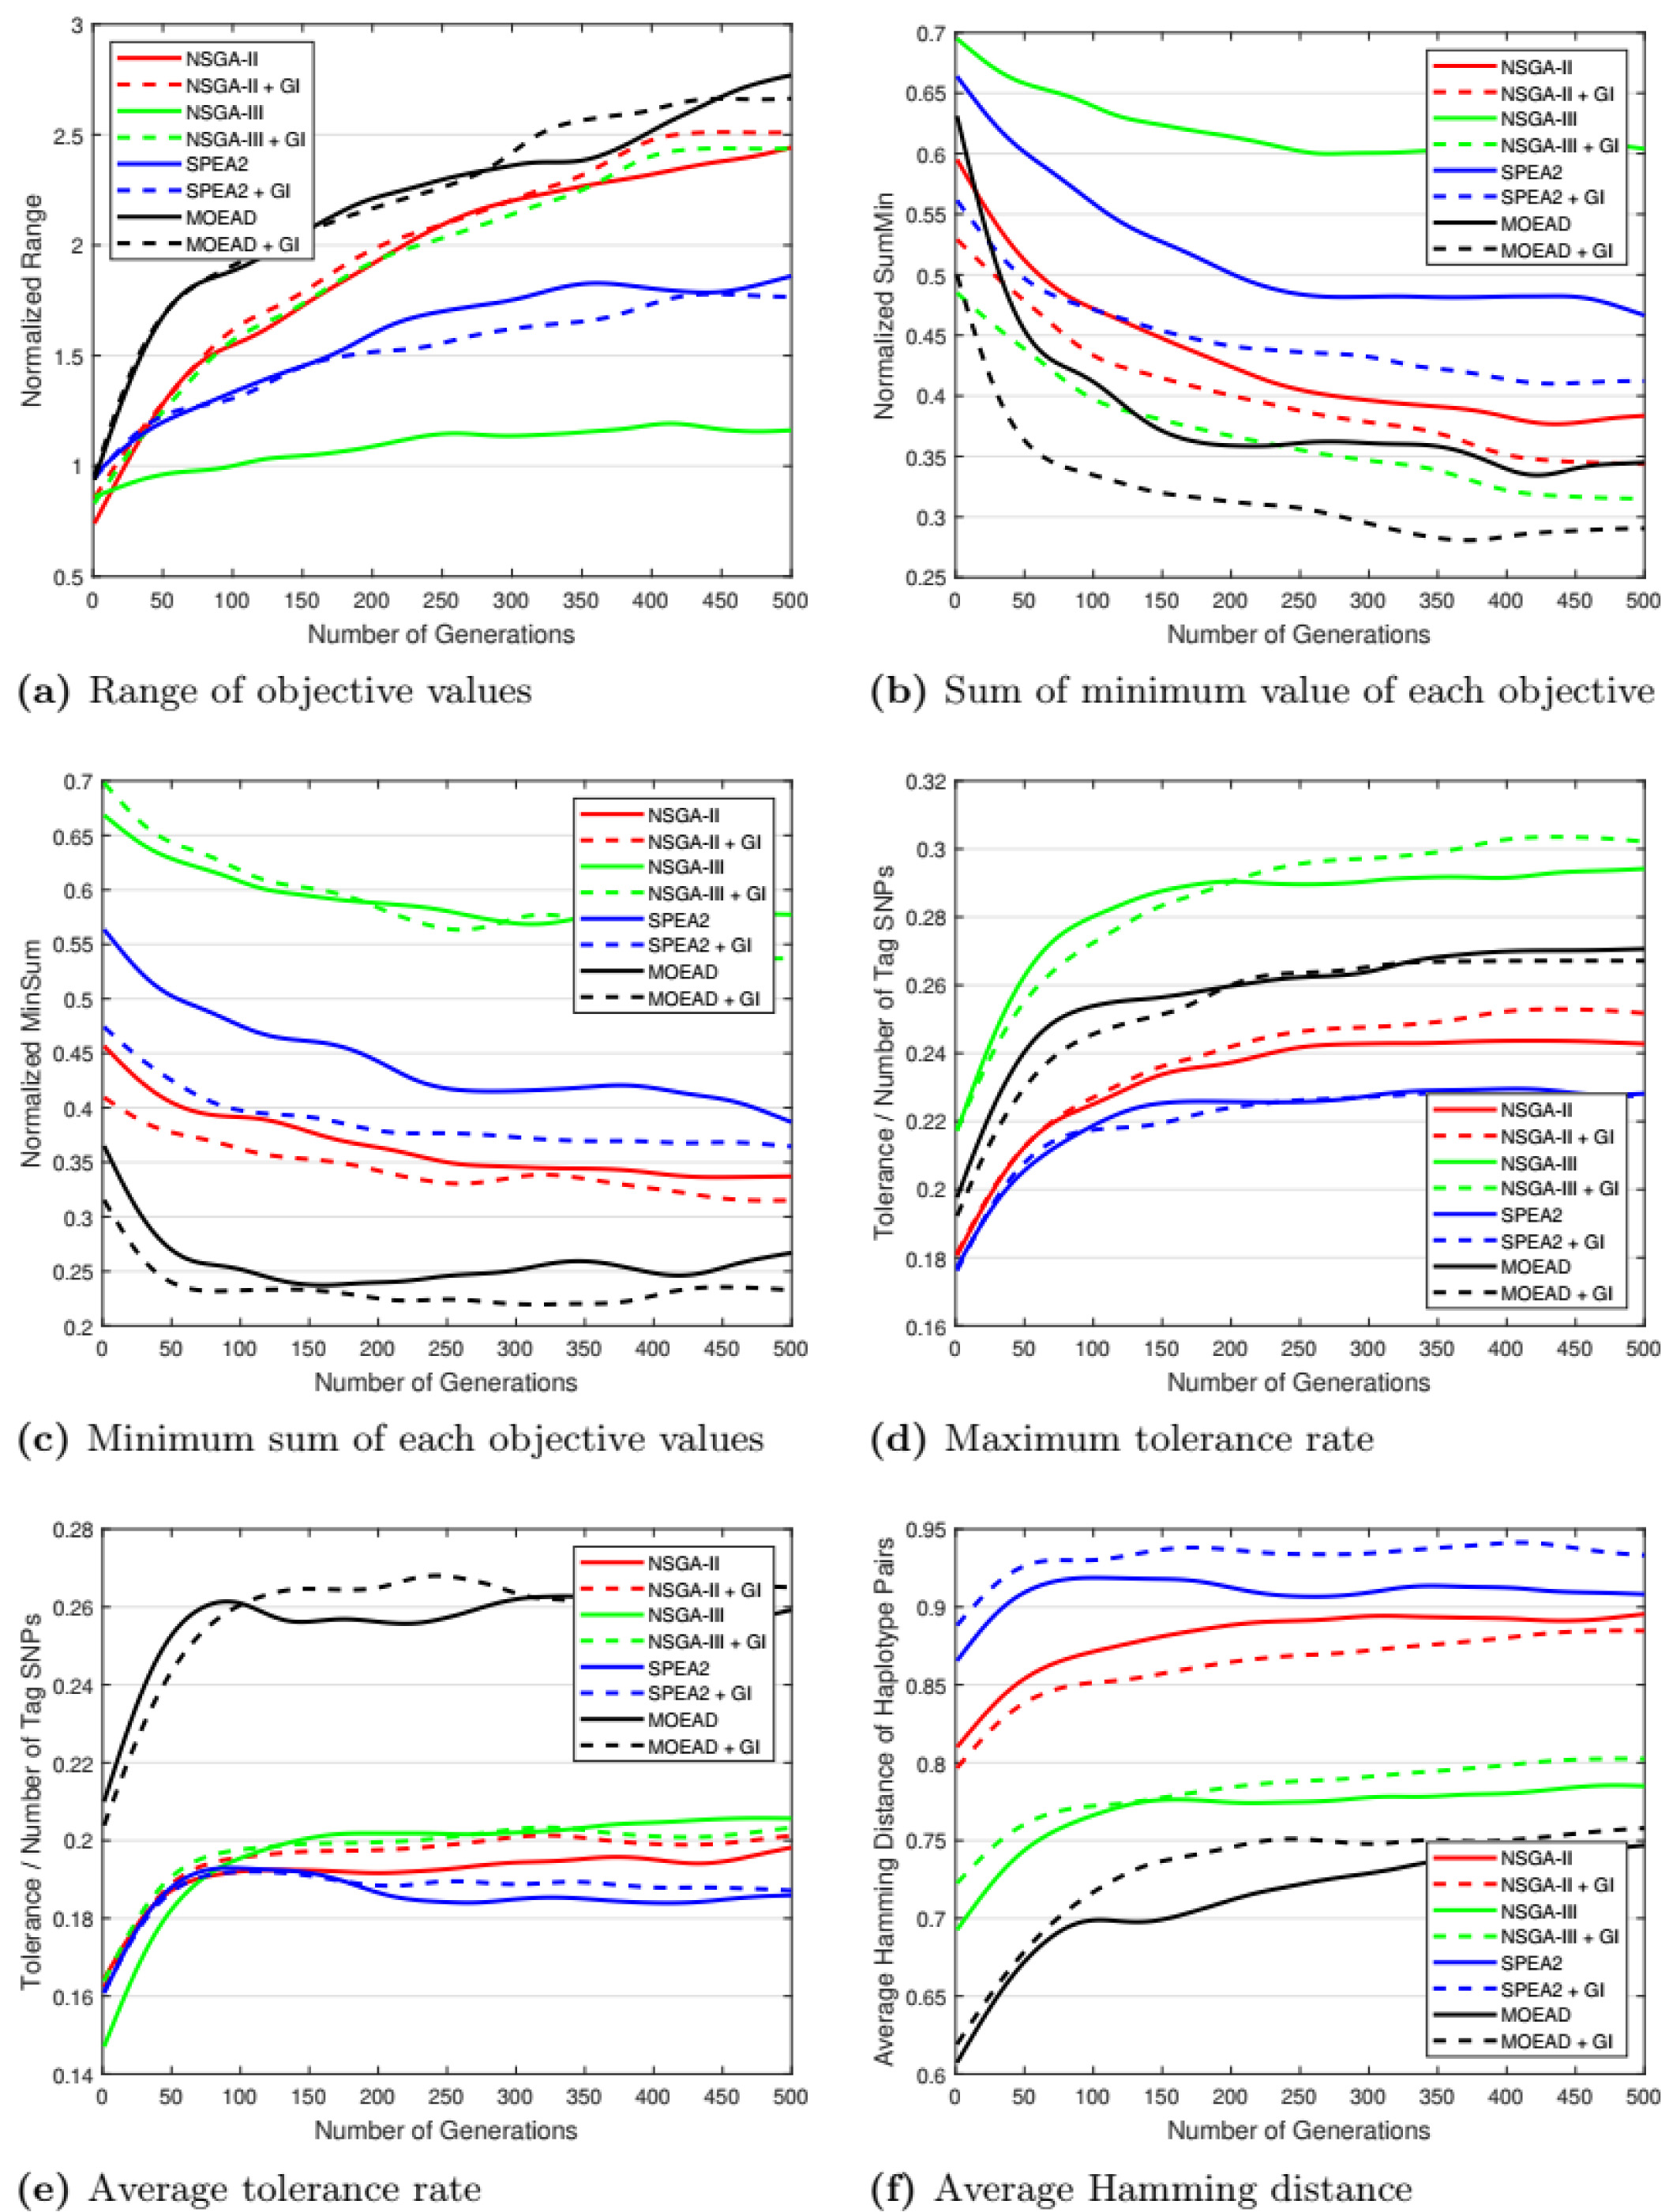
\includegraphics[width=\textwidth]{analisis_assets/moqa_2022/figures/moqa_fig_convergencia_1.jpeg}
        \caption{Evolución por generación de seis métricas de rendimiento en el experimento base (500 generaciones, población = 200). Se ilustra el impacto de la inicialización heurística (GI, líneas discontinuas) frente a la aleatoria (RI, líneas continuas).}
    \end{subfigure}
    \hfill
    \begin{subfigure}[b]{0.48\textwidth}
        \centering
        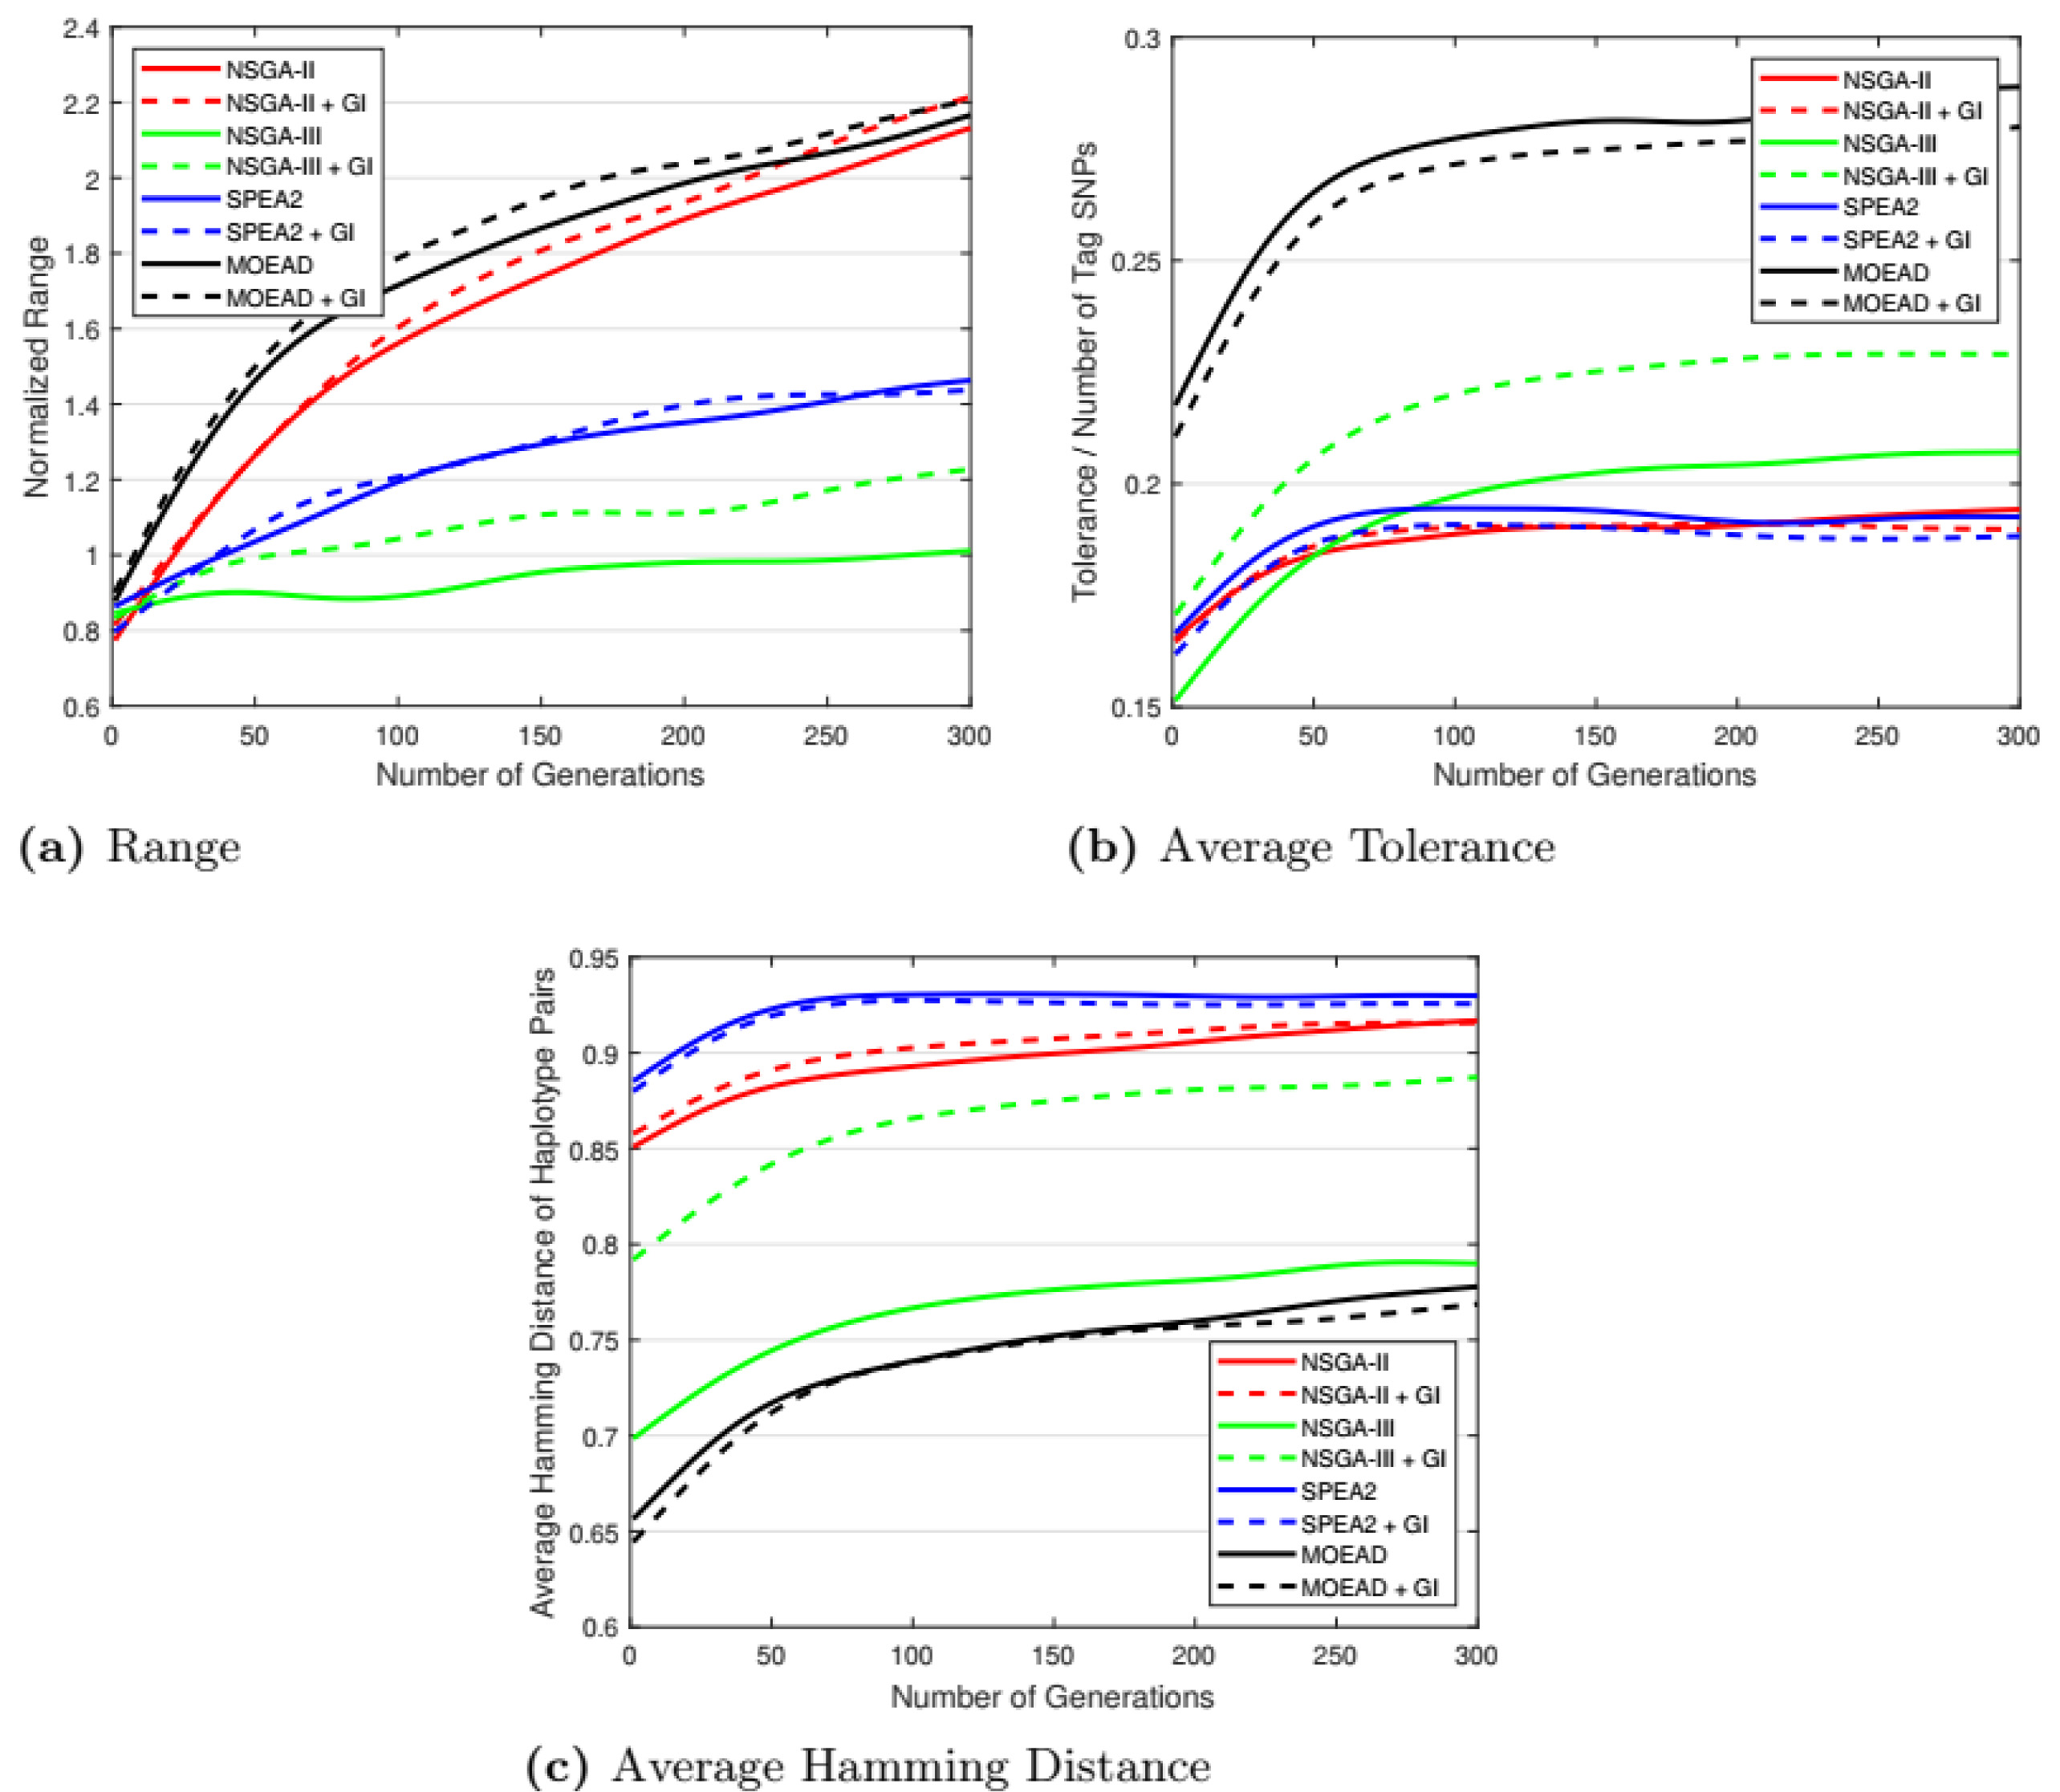
\includegraphics[width=\textwidth]{analisis_assets/moqa_2022/figures/moqa_fig_convergencia_2.jpeg}
        \caption{Estudio de sensibilidad de parámetros genéticos (300 generaciones, población = 100). Análisis focalizado en la robustez de los algoritmos ante una reducción de recursos computacionales.}
    \end{subfigure}
    \caption{Análisis de las trayectorias de convergencia reportadas por Moqa et al. (2022).}
\end{figure}

\subsubsection{Top 10 por métrica (Moqa)}
A continuación se presentan los valores finales extraídos de las gráficas de convergencia del estudio original. Estos datos representan el rendimiento absoluto alcanzado en la generación 500.

\subparagraph{Top 10: Range ($\uparrow$)}
\begin{table}[H]
    \centering
    \begin{tabular}{cllc}
        \toprule
        Pos & Algoritmo & Inicialización & Valor ($\mu \pm \sigma$) \\
        \midrule
        1 & MOEAD & R & 2.75 $\pm$ 0.3981 \\
        2 & MOEAD & G & 2.60 $\pm$ 0.4080 \\
        3 & NSGA2 & G & 2.50 $\pm$ 0.4522 \\
        4 & NSGA2 & R & 2.45 $\pm$ 0.4359 \\
        5 & NSGA3 & G & 2.45 $\pm$ 0.4390 \\
        6 & SPEA2 & R & 1.80 $\pm$ 0.2499 \\
        7 & SPEA2 & G & 1.75 $\pm$ 0.2128 \\
        8 & NSGA3 & R & 1.10 $\pm$ 0.0923 \\
        \bottomrule
    \end{tabular}
    \caption{Top para Range en el reporte de Moqa (Valores extraídos de gráfica).}
\end{table}

\subparagraph{Top 10: SumMin ($\downarrow$)}
\begin{table}[H]
    \centering
    \begin{tabular}{cllc}
        \toprule
        Pos & Algoritmo & Inicialización & Valor ($\mu \pm \sigma$) \\
        \midrule
        1 & MOEAD & G & 0.29 $\pm$ 0.0435 \\
        2 & NSGA3 & G & 0.32 $\pm$ 0.0443 \\
        3 & MOEAD & R & 0.35 $\pm$ 0.0603 \\
        4 & NSGA2 & G & 0.35 $\pm$ 0.0483 \\
        5 & NSGA2 & R & 0.38 $\pm$ 0.0542 \\
        6 & SPEA2 & G & 0.41 $\pm$ 0.0354 \\
        7 & SPEA2 & R & 0.46 $\pm$ 0.0506 \\
        8 & NSGA3 & R & 0.60 $\pm$ 0.0249 \\
        \bottomrule
    \end{tabular}
    \caption{Top para SumMin en el reporte de Moqa (Valores extraídos de gráfica).}
\end{table}

\subparagraph{Top 10: MinSum ($\downarrow$)}
\begin{table}[H]
    \centering
    \begin{tabular}{cllc}
        \toprule
        Pos & Algoritmo & Inicialización & Valor ($\mu \pm \sigma$) \\
        \midrule
        1 & MOEAD & G & 0.23 $\pm$ 0.0179 \\
        2 & MOEAD & R & 0.27 $\pm$ 0.0238 \\
        3 & NSGA2 & G & 0.32 $\pm$ 0.0229 \\
        4 & NSGA2 & R & 0.34 $\pm$ 0.0296 \\
        5 & SPEA2 & G & 0.37 $\pm$ 0.0252 \\
        6 & SPEA2 & R & 0.39 $\pm$ 0.0404 \\
        7 & NSGA3 & G & 0.54 $\pm$ 0.0390 \\
        8 & NSGA3 & R & 0.57 $\pm$ 0.0243 \\
        \bottomrule
    \end{tabular}
    \caption{Top para MinSum en el reporte de Moqa (Valores extraídos de gráfica).}
\end{table}

\subparagraph{Top 10: Max. Tolerance Rate ($\uparrow$)}
\begin{table}[H]
    \centering
    \begin{tabular}{cllc}
        \toprule
        Pos & Algoritmo & Inicialización & Valor ($\mu \pm \sigma$) \\
        \midrule
        1 & NSGA3 & G & 0.30 $\pm$ 0.0204 \\
        2 & NSGA3 & R & 0.29 $\pm$ 0.0160 \\
        3 & MOEAD & R & 0.275 $\pm$ 0.0149 \\
        4 & MOEAD & G & 0.27 $\pm$ 0.0173 \\
        5 & NSGA2 & G & 0.25 $\pm$ 0.0170 \\
        6 & NSGA2 & R & 0.24 $\pm$ 0.0146 \\
        7 & SPEA2 & G & 0.23 $\pm$ 0.0108 \\
        8 & SPEA2 & R & 0.23 $\pm$ 0.0113 \\
        \bottomrule
    \end{tabular}
    \caption{Top para Max. Tolerance Rate en el reporte de Moqa (Valores extraídos de gráfica).}
\end{table}

\subparagraph{Top 10: Avg. Tolerance Rate ($\uparrow$)}
\begin{table}[H]
    \centering
    \begin{tabular}{cllc}
        \toprule
        Pos & Algoritmo & Inicialización & Valor ($\mu \pm \sigma$) \\
        \midrule
        1 & MOEAD & R & 0.26 $\pm$ 0.0099 \\
        2 & MOEAD & G & 0.26 $\pm$ 0.0130 \\
        3 & NSGA3 & R & 0.21 $\pm$ 0.0120 \\
        4 & NSGA3 & G & 0.21 $\pm$ 0.0075 \\
        5 & NSGA2 & G & 0.20 $\pm$ 0.0075 \\
        6 & NSGA2 & R & 0.20 $\pm$ 0.0060 \\
        7 & SPEA2 & G & 0.19 $\pm$ 0.0054 \\
        8 & SPEA2 & R & 0.19 $\pm$ 0.0056 \\
        \bottomrule
    \end{tabular}
    \caption{Top para Avg. Tolerance Rate en el reporte de Moqa (Valores extraídos de gráfica).}
\end{table}

\subparagraph{Top 10: Avg. Hamming ($\uparrow$)}
\begin{table}[H]
    \centering
    \begin{tabular}{cllc}
        \toprule
        Pos & Algoritmo & Inicialización & Valor ($\mu \pm \sigma$) \\
        \midrule
        1 & SPEA2 & G & 0.94 $\pm$ 0.0098 \\
        2 & SPEA2 & R & 0.91 $\pm$ 0.0094 \\
        3 & NSGA2 & R & 0.90 $\pm$ 0.0191 \\
        4 & NSGA2 & G & 0.87 $\pm$ 0.0195 \\
        5 & NSGA3 & G & 0.80 $\pm$ 0.0177 \\
        6 & NSGA3 & R & 0.78 $\pm$ 0.0191 \\
        7 & MOEAD & G & 0.76 $\pm$ 0.0326 \\
        8 & MOEAD & R & 0.75 $\pm$ 0.0309 \\
        \bottomrule
    \end{tabular}
    \caption{Top para Avg. Hamming en el reporte de Moqa (Valores extraídos de gráfica).}
\end{table}

\subsubsection{Ranking Promedio (Average Rank)}
El análisis del ranking global mediante el método \textit{Average Rank} (promedio de las posiciones obtenidas en las 6 métricas reportadas) permite identificar las configuraciones más equilibradas del estudio original con una métrica estadísticamente más robusta.

\begin{table}[H]
    \centering
    \begin{tabular}{lllc}
        \toprule
        Pos & Algo & Init & Avg. Rank (Friedman) \\
        \midrule
        1 & MOEAD & G \\
        2 & MOEAD & R \\
        3 & NSGA3 & G \\
        4 & NSGA2 & G \\
        5 & NSGA2 & R \\
        6 & SPEA2 & G \\
        7 & NSGA3 & R \\
        8 & SPEA2 & R \\
        \bottomrule
    \end{tabular}
    \caption{Ranking Global (Average Rank) para el reporte de Moqa et al. (2022). Un \textbf{valor menor} indica un desempeño superior.}
\end{table}

\subsubsection{Conclusiones del Reporte Moqa}
 \begin{itemize}
     \item \textbf{Mejores métodos:} El análisis mediante \textit{Average Rank} sitúa a \textbf{MOEA/D+G} en la \textbf{primera posición} del ranking global de Moqa, seguido por \textbf{MOEA/D+R}. Esto respalda, en términos ordinales, la robustez de los algoritmos basados en descomposición en el estudio original.
     \item \textbf{Mejores inicializaciones:} La inicialización \textbf{Greedy (G)} tiende a ocupar posiciones superiores frente a variantes aleatorias, especialmente en combinaciones con MOEA/D y NSGA-III, según el ranking promedio.
     \item \textbf{Otros apuntes a destacar:} A nivel de métricas individuales, \textbf{SPEA2} destaca en el ranking de diversidad (\textit{Avg. Hamming Distance}) dentro del reporte original, lo cual motiva su consideración cuando la variabilidad de Tag SNPs es prioritaria.
 \end{itemize}

\subsubsection{Comparativa con las Conclusiones de los Autores}
Al contrastar el análisis del TFG con las declaraciones literales de Moqa et al. (2022), se procede a la validación de sus conclusiones fundamentales:

\begin{itemize}
    \item \textbf{Superioridad de los algoritmos de muchos objetivos:} Los autores sostienen que MOEA/D y NSGA-III ofrecen un rendimiento superior a NSGA-II y SPEA2. Se valida íntegramente para MOEA/D (posiciones 1 y 2 del ranking). En el caso de NSGA-III, la superioridad se valida únicamente bajo inicialización heurística (G, posición 3), mientras que bajo inicialización aleatoria su desempeño decae drásticamente.
    \item \textbf{Liderazgo de MOEA/D:} Afirman que MOEA/D supera al resto en la mayoría de los casos. Se valida de forma absoluta, ya que tanto MOEA/D+G como MOEA/D+R encabezan el \textit{Average Rank} global, demostrando ser la arquitectura más robusta para este problema.
    \item \textbf{Impacto de la inicialización Greedy:} Sostienen que la inicialización heurística mejora los resultados para NSGA-III, SPEA2 y MOEA/D. Se valida categóricamente; el ranking muestra una mejora sistemática en los rangos promedio al emplear G frente a R para todos los algoritmos citados.
    \item \textbf{Validación de la diversidad en SPEA2:} A pesar de no ser el más equilibrado globalmente, se mantiene la validación de la afirmación específica de los autores sobre la superioridad de SPEA2 en la preservación de la distancia de Hamming, una vez analizados los valores finales de las gráficas.
\end{itemize}


% =========================================================
\section{Análisis de las ejecuciones propias}
\label{sec:mis_experimentos}

\subsection{Configuración}

\subsubsection{Configuración común}
A continuación se detallan los parámetros y configuraciones compartidas por las ejecuciones A y B de este reporte. Aquellos aspectos que varían entre ejecuciones se señalizan explícitamente como \guillemotleft NO COMÚN\guillemotright.

\begin{itemize}
    \item \textbf{Infraestructura:} Implementada mediante la librería especializada \textbf{pymoo} (Python).
    \item \textbf{Dataset:} Benchmark biológico Hinds 2005. Se utilizan 772 marcadores genéticos (SNPs) polimórficos tras filtrar los 1032 originales, con una estructura de 48 patrones alélicos.
    \item \textbf{Configuración Global:}
    \begin{itemize}
        \item \textbf{Transformación de objetivos (NO COMÚN):} 
        \begin{itemize}
            \item \textbf{Ejecución A:} Negación lineal ($f' = -f$) para convertir la maximización en minimización sin distorsionar el espacio biológico.
            \item \textbf{Ejecución B:} Inversión no lineal ($1/f$) para objetivos de maximización ($f_2$ y $f_3$).
        \end{itemize}
        \item \textbf{Normalización (Min-Max):} Escalado estático mediante el modo \textbf{\texttt{static\_proportional\_limits}}. A diferencia de la normalización dinámica, esta técnica emplea límites fijos basados en la naturaleza proporcional de los objetivos (inspirado en Ting, 2010), proyectando la distancia de Hamming media hacia el intervalo $[0, 1]$ y su varianza hacia $[0, \mbox{0.25}]$. Esta aproximación garantiza un hipercubo de referencia estable para el cálculo del Hipervolumen, permitiendo comparativas matemáticamente rigurosas entre diferentes algoritmos y ejecuciones.
    \end{itemize}
    \item \textbf{Parámetros de los Algoritmos:}
    \begin{itemize}
        \item \textbf{Ajustes generales:} Tamaño de la población de 200 individuos, 500 generaciones, 200 descendientes, 5 ejecuciones independientes, Cruce Uniforme (70\%) y Mutación $1/L \approx 0,0013$.
        \item \textbf{Ajustes específicos de NSGA-III:} 9 particiones por objetivo (200 direcciones de referencia).
        \item \textbf{Otros Algoritmos:} NSGA-II y SPEA2 basados en dominancia; MOEA/D con vecindario de 15 y penalización PBI de 5.0.
    \end{itemize}
    \item \textbf{Estrategias de Inicialización:} Se evalúan cuatro enfoques, diseñados para cubrir un espectro amplio de densidad inicial y sesgo heurístico:
    \begin{itemize}
        \item \textbf{\texttt{random\_sparse} (baja densidad):} Genera soluciones iniciales con una fracción pequeña de SNPs seleccionados (aprox. 9\%). Favorece la \textbf{exploración} y la diversidad combinatoria, pero suele partir de soluciones menos representativas biológicamente, por lo que el algoritmo debe invertir más esfuerzo en mejorar la cobertura.
        \item \textbf{\texttt{random\_dense} (densidad media-alta):} Inicializa con una fracción elevada de SNPs (aprox. 50\%). Proporciona un punto de partida con mayor \textbf{cobertura biológica} y, en ocasiones, una convergencia más estable en métricas de tolerancia, a costa de introducir un sesgo hacia soluciones densas que puede dificultar la reducción posterior.
        \item \textbf{\texttt{greedy\_ting} (heurística inspirada en Ting, 2010):} Construye semillas con un esquema \textbf{voraz} guiado por la representatividad, incorporando mecanismos de \textbf{diversificación por grupos} para evitar soluciones degeneradas. Su objetivo es partir de soluciones ya competitivas sin sacrificar completamente la variedad estructural de la población.
        \item \textbf{\texttt{greedy\_hybrid} (mixta 50/50):} Combina sistemáticamente una mitad de individuos sembrados con heurística Greedy y otra mitad aleatoria. Este compromiso busca equilibrar \textbf{explotación temprana} (semillas fuertes) y \textbf{exploración} (variabilidad), reduciendo la dependencia del algoritmo respecto a un único tipo de punto de partida.
    \end{itemize}
\end{itemize}

\subsubsection{Profundización en la configuración}

\paragraph{Estrategias de Inicialización de la Población}
La calidad del conjunto inicial de soluciones es un factor crítico en el rendimiento de los algoritmos evolutivos para la selección de Tag SNPs. En este trabajo, el motor de optimización se ha equipado con un abanico de estrategias que oscilan desde la estocasticidad pura hasta la inyección de heurísticas altamente especializadas. El objetivo es ofrecer herramientas que permitan modular la densidad inicial del cromosoma y el grado de conocimiento experto (sesgo constructivo) con el que arranca la búsqueda.

\textbf{1. \texttt{random\_sparse} (Aleatoria Dispersa)} \\
Este enfoque genera soluciones aleatorias pero imponiendo una drástica restricción sobre la cantidad de SNPs que se activan al inicio. El algoritmo no utiliza una probabilidad fija del 50\%, sino que calcula una probabilidad dinámica de inserción inversamente proporcional a la longitud del cromosoma ($p \approx 70 / n\_var$), garantizando un techo del 50\% y un suelo del 1\%. Además, la implementación cuenta con un mecanismo de seguridad para evitar que se inyecten individuos completamente vacíos en la población (0 SNPs activos), forzando la activación de al menos un gen en casos extremos.
\begin{itemize}
    \item \textit{Ejemplo conceptual:} Si el bloque genómico consta de 1000 SNPs, esta estrategia generará cromosomas iniciales con aproximadamente 70 SNPs seleccionados al azar. Esto obliga al algoritmo evolutivo a partir de frentes con un bajo coste biológico (pocos marcadores) y le cede toda la responsabilidad exploratoria de ir descubriendo e incorporando aquellos SNPs que mejoren la cobertura de forma sinérgica, favoreciendo una construcción "hacia arriba".
\end{itemize}

\textbf{2. \texttt{random\_dense} (Aleatoria Densa)} \\
Se trata del muestreo estocástico binario estándar. A cada SNP del cromosoma se le asigna una probabilidad equitativa ($p=0,50$) de ser seleccionado de forma independiente mediante una distribución uniforme. A diferencia de \texttt{random\_sparse}, no busca economía en el tamaño del panel inicial, sino una cobertura masiva desde el primer momento.
\begin{itemize}
    \item \textit{Ejemplo conceptual:} En el mismo escenario de 1000 SNPs, cada individuo de la población inicial arrancará con una media de 500 SNPs marcados. Esta sobreabundancia de marcadores asegura, estadísticamente, que casi todos los haplotipos de la muestra puedan ser distinguidos entre sí desde la generación 0 (alcanzando altas cotas iniciales en métricas como tolerancia y alcance). Sin embargo, sitúa una enorme presión evolutiva sobre los operadores de mutación y cruce, que tendrán que podar masivamente los cromosomas para alcanzar soluciones óptimas en tamaño.
\end{itemize}

\textbf{3. \texttt{greedy\_ting} (Heurística Compleja inspirada en Ting)} \\
Esta inicialización representa la inyección más profunda de conocimiento experto en el genoma inicial, estructurada en múltiples fases deterministas y probabilísticas. En primer lugar, la matriz de haplotipos es pre-evaluada para calcular un \textit{Balance Alélico} para cada SNP (priorizando aquellos cuya frecuencia alélica se aproxima al 50\%, ya que dividen la población de forma más equilibrada). A continuación, el algoritmo agrupa los SNPs en ``bloques de cobertura idéntica'' (SNPs que biológicamente resuelven exactamente los mismos pares de haplotipos). 
La población se conforma rellenando porcentajes específicos:
\begin{enumerate}
    \item Un subconjunto de semillas ancla calculadas de forma determinista, cuya cantidad se define mediante la expresión $\text{Total Anclas} = 2 \times \lceil \frac{\lceil ratio\_greedy \times 10 \rceil}{2} \rceil$. En esta fase se alternan copias de la \textit{Semilla Greedy} (mínimo de marcadores para cobertura total según el balance alélico) y la \textit{Semilla Densa} (totalidad de SNPs con firma única identificados).
    \item Individuos generados mediante un muestreo voraz por grupos funcionales, donde se selecciona un único representante al azar por cada bloque de cobertura hasta resolver la red de pares de haplotipos.
    \item Individuos donde se activa exactamente un representante al azar por cada grupo funcional de forma estricta, independientemente de la redundancia o cobertura final alcanzada.
    \item El remanente de la población se rellena mediante muestreo aleatorio denso (distribución de Bernoulli con $p=0,50$).
\end{enumerate}
\begin{itemize}
    \item \textit{Ejemplo de ejecución paso a paso:} \\
    Para ilustrar la mecánica interna de esta estrategia, se plantea un escenario con una población de $N=20$ individuos y un \texttt{ratio\_greedy} de $0,5$ (donde el 50\% de la población se construye mediante heurísticas especializadas y el resto mediante muestreo aleatorio). Se parte de tres grupos funcionales de cobertura: Grupo A $\{S_1, S_4\}$, Grupo B $\{S_2\}$ y Grupo C $\{S_3\}$, con un orden de prioridad basado en el balance alélico de $[S_1, S_2, S_3]$.
    
    El proceso de construcción se divide en tres fases secuenciales:

    \textbf{Fase 1: Inyección de Puntos Ancla (Individuos 1 al 6)} \\
    El algoritmo asegura la presencia de copias de las plantillas base de mayor calidad. El número de anclas se deriva del ratio configurado mediante la expresión $\text{Total Anclas} = 2 \times \lceil \frac{\lceil ratio\_greedy \times 10 \rceil}{2} \rceil$. En este caso ($ratio\_greedy=0,5$), se inyectan 6 individuos alternando las dos semillas maestras:
    \begin{itemize}
        \item \textbf{Individuos 1, 3 y 5:} Semilla Greedy $\rightarrow \{S_1, S_2\}$ (mínima cantidad de marcadores para cobertura total según el orden de prioridad).
        \item \textbf{Individuos 2, 4 y 6:} Semilla Densa $\rightarrow \{S_1, S_2, S_3\}$ (totalidad de SNPs únicos identificados en el orden de prioridad).
    \end{itemize}

    \textbf{Fase 2: Relleno Heurístico por Grupos (Individuos 7 al 10)} \\
    Una vez satisfecho el cupo de anclas, las posiciones restantes del bloque heurístico (hasta completar los 10 individuos del 50\%) se completan alternando técnicas de muestreo sobre los grupos funcionales para inyectar diversidad biológica informada:
    \begin{itemize}
        \item \textbf{Individuos 7 y 9 (Muestreo Greedy):} El algoritmo permuta el orden de los grupos y selecciona un representante al azar por cada uno únicamente si existen pares de haplotipos aún no resueltos. Por ejemplo, la construcción podría resultar en $\rightarrow \{S_4, S_2\}$.
        \item \textbf{Individuos 8 y 10 (Muestreo Unique):} Se selecciona obligatoriamente un SNP de cada grupo funcional con independencia del estado de cobertura, garantizando la representatividad estructural de todas las regiones informativas del genoma $\rightarrow \{S_4, S_2, S_3\}$.
    \end{itemize}

    \textbf{Fase 3: Relleno Aleatorio (Individuos 11 al 20)} \\
    El 50\% restante de la población se genera mediante una distribución de Bernoulli independiente para cada gen. Cada SNP tiene una probabilidad $p=0,50$ de ser activado, proporcionando un sustrato de variabilidad estocástica no sesgada:
    \begin{itemize}
        \item \textbf{Individuo 11...20:} Generan patrones heterogéneos como $\{S_2, S_4\}$ o soluciones altamente redundantes como $\{S_1, S_2, S_3, S_4\}$.
    \end{itemize}
    
    Esta arquitectura garantiza que la búsqueda evolutiva comience con un núcleo de soluciones óptimas (Fase 1), variaciones estructurales coherentes (Fase 2) y una base de diversidad necesaria para evitar la convergencia prematura (Fase 3).
\end{itemize}

\textbf{4. \texttt{greedy\_hybrid} (Mixta 50/50)} \\
Diseñada para maximizar el equilibrio entre la explotación del conocimiento heurístico y la pura exploración estocástica, esta estrategia divide la población rigurosamente en dos mitades (50/50). 

La primera mitad de los individuos se construye utilizando un esquema voraz iterativo: se evalúa la \textit{capacidad de discriminación} individual de cada SNP frente a los pares de haplotipos que aún no han sido resueltos en ese momento, seleccionándolos en orden descendente hasta cubrir toda la red. 

Para evitar que toda esta primera mitad converja en clones exactos, la heurística agrupa los SNPs con idéntico poder discriminatorio y baraja aleatoriamente su orden interno antes de evaluarlos, inyectando estocasticidad en los desempates. 

La segunda mitad de la población se rellena utilizando el enfoque exploratorio de baja densidad (\texttt{random\_sparse}).
\begin{itemize}
    \item \textit{Ejemplo de ejecución paso a paso:} \\
    La estrategia \texttt{greedy\_hybrid} opera mediante un esquema bimodal que integra una heurística de distinción y un muestreo estocástico disperso. Para ilustrar su funcionamiento, se define un panel de 4 SNPs ($S_1$ a $S_4$) para generar una población de $N=4$ individuos con un \texttt{ratio\_greedy} del 50\%.
    
    \textbf{Fase 1: Análisis de Distinguibilidad y Agrupamiento} \\
    El algoritmo evalúa la capacidad individual de cada SNP para diferenciar los pares de haplotipos mediante la función \texttt{calcular\_distinguibilidad\_snps}. Supongamos que $S_1$ y $S_2$ distinguen 5 pares cada uno, mientras que $S_3$ y $S_4$ distinguen 3 pares. Basándose en estos valores, el sistema organiza los marcadores en grupos de prioridad:
    \begin{itemize}
        \item \textbf{Grupo A (Prioridad alta):} $\{S_1, S_2\}$.
        \item \textbf{Grupo B (Prioridad media):} $\{S_3, S_4\}$.
    \end{itemize}
    Se determina la construcción de 2 individuos mediante heurística voraz y 2 mediante muestreo aleatorio.

    \textbf{Fase 2: Construcción del Bloque Heurístico (Individuos 1 y 2)} \\
    Para cada individuo de esta fase, se ejecuta una construcción voraz asistida por un mecanismo de desempate aleatorio sobre los grupos de prioridad. Esto asegura que, aunque compartan la misma lógica de optimización, las trayectorias genéticas puedan divergir:
    \begin{itemize}
        \item \textbf{Individuo 1:} Se permuta internamente el Grupo A como $[S_2, S_1]$ y el Grupo B como $[S_4, S_3]$. El motor de construcción selecciona $S_2$ y, al no alcanzar cobertura total, incorpora $S_1$. Al cubrirse todos los pares, la solución finaliza $\rightarrow \{S_1, S_2\}$.
        \item \textbf{Individuo 2:} Una nueva permutación resulta en el orden $[S_1, S_2, S_3, S_4]$. Siguiendo el mismo procedimiento, la solución converge nuevamente en $\rightarrow \{S_1, S_2\}$. En instancias reales con miles de variables, este proceso genera una variabilidad estructural significativa entre individuos de alta aptitud.
    \end{itemize}

    \textbf{Fase 3: Relleno Estocástico Disperso (Individuos 3 y 4)} \\
    Los individuos restantes se generan ignorando las métricas de distinguibilidad biológica, utilizando una distribución de Bernoulli con una probabilidad de activación (\texttt{prob\_aleatoria}):
    \begin{itemize}
        \item \textbf{Individuo 3:} El muestreo independiente resulta en la activación de $S_2$ y $S_3 \rightarrow \{S_2, S_3\}$.
        \item \textbf{Individuo 4:} Supongamos que el proceso estocástico no activa ningún marcador. El sistema aplica una cláusula de seguridad para evitar soluciones degeneradas, forzando la selección de un SNP al azar (ej. $S_4$) $\rightarrow \{S_4\}$.
    \end{itemize}
    
    El resultado es una población que equilibra la explotación de soluciones casi óptimas con un sustrato de variabilidad estocástica, facilitando el trabajo de los operadores evolutivos en generaciones posteriores.
\end{itemize}

\paragraph{Normalización Min-Max}
El sistema aplica una normalización de objetivos al espacio $[0, 1]$ para el cálculo de indicadores agregados mediante una proyección Min-Max:
\begin{equation}
\label{eq:norm_common}
F_{norm} = \frac{f - f_{ideal}}{f_{nadir} - f_{ideal}}
\end{equation}

\paragraph{Normalización Static Proportional Limits}
Para garantizar la integridad académica y la comparabilidad entre ejecuciones, se emplea el modo \\ \mbox{\textbf{\texttt{static\_proportional\_limits}}}. A diferencia de la normalización dinámica (que reajusta los límites $f_{ideal}$ y $f_{nadir}$ en cada generación), esta técnica utiliza cotas teóricas fijas derivadas de la naturaleza proporcional del problema (Ting, 2010):

\begin{itemize}
    \item \textbf{Distancia de Hamming ($f_3$):} Se proyecta hacia el intervalo $[0, 1]$.
    \item \textbf{Varianza de Hamming ($f_4$):} Se proyecta hacia el intervalo $[0, \mbox{0.25}]$.
\end{itemize}

\paragraph{Ejemplo de cálculo para el Reporte A (Modo negación)}
Se analiza una solución en la que la distancia de Hamming media capturada es el 40\% del máximo teórico ($p=0,40$). Bajo la transformación de negación del Reporte A, el valor del objetivo es $f_3 = -0,40$. Aplicando los límites estáticos de normalización ($f_{ideal} = -1,0$ y $f_{nadir} = 0,0$):
\begin{equation}
F_{norm} = \frac{-0,40 - (-1,0)}{0,0 - (-1,0)} = \frac{0,60}{1,0} = \mathbf{0,60}
\end{equation}
\textbf{Interpretación:} El valor 0,60 en el espacio normalizado indica que la solución se encuentra al 60\% de distancia del ideal de diversidad, proporcionando una métrica de convergencia estequiométrica y comparable.

Esta estabilidad es fundamental para el cálculo del \textbf{Hipervolumen (HV)}. Al mantener los límites constantes, el \textit{Reference Point} ($1.1$) permanece anclado a un hipercubo de referencia invariable. Esto asegura que una mejora en el HV represente un avance real en la calidad del frente y no un artefacto estadístico provocado por el desplazamiento de los límites de normalización durante la evolución.

\paragraph{Nota metodológica sobre la comparabilidad}
La Ejecución \textbf{A} utiliza una transformación de objetivos mediante negación (\texttt{neg}), mientras que la Ejecución \textbf{B} emplea inversión (\texttt{inverse}). Por lo tanto, los valores agregados de A y B \textbf{no son comparables directamente por su magnitud bruta}. La comparativa debe centrarse en el \textbf{ranking relativo} de los algoritmos dentro de cada entorno y en los valores decodificados cuando proceda.

\textit{Guía de Comparabilidad:}
\begin{itemize}
    \item \textbf{Métricas NO comparables (en valor absoluto):} No deben compararse cuantitativamente entre A y B debido a que dependen de la topología del espacio transformado.
    \begin{itemize}
        \item \textbf{Hypervolume (HV):} Mide volúmenes en espacios con naturalezas distintas (lineal vs. recíproca).
        \item \textbf{SumMin y MinSum:} Agregados basados en sumas de valores negativos vs. inversos.
        \item \textbf{Range:} La dispersión se ve alterada por la compresión asintótica de la inversión.
    \end{itemize}
    \item \textbf{Métricas SÍ comparables (directamente):} Indicadores robustos que preservan su significado físico o estadístico.
    \begin{itemize}
        \item \textbf{Valores Biológicos Decodificados:} Tasa de Tolerancia real, Distancia de Hamming y número de SNPs.
        \item \textbf{Ranking Relativo y Global Rank-Sum:} La posición ordinal de los algoritmos es una medida universal de desempeño relativo.
    \end{itemize}
\end{itemize}

\subsection{Reporte 2 — Ejecución A: 20260430T185224}
\label{sec:reporte2}

\subsubsection{Configuración específica}
Esta ejecución utiliza la transformación de objetivos por \textbf{negación} (\texttt{neg}), donde $f' = -f$. Se evalúan las mismas estrategias de inicialización definidas en la configuración común (\texttt{random\_sparse}, \texttt{random\_dense}, \texttt{greedy\_ting} y \texttt{greedy\_hybrid}).

\subsubsection{Resultados y análisis (A)}

\subsubsection{Frente de Pareto Global}
\begin{figure}[H]
    \centering
    
\includegraphics[width=0.6\textwidth]{analisis_assets/20260430T185224/2_comparativa/1_frentes/frentes_pareto/frentes_pareto_global_full.png}
    \caption{Frente de Pareto Global consolidado para la Ejecución A.}
\end{figure}

\subsubsection{Frentes de Pareto (Convergencia final)}

\begin{table}[H]
    \centering
    \begin{tabular}{m{2.2cm} >{\centering\arraybackslash}m{3.2cm} >{\centering\arraybackslash}m{3.2cm} >{\centering\arraybackslash}m{3.2cm} >{\centering\arraybackslash}m{3.2cm}}
        \toprule
        Algoritmo & random\_sparse & random\_dense & greedy\_ting & greedy\_hybrid \\
        \midrule
        \textbf{NSGA-II} & 
\includegraphics[width=\linewidth]{analisis_assets/20260430T185224/2_comparativa/1_frentes/frentes_pareto/frentes_pareto_nsga2_random_sparse_full.png} & 
\includegraphics[width=\linewidth]{analisis_assets/20260430T185224/2_comparativa/1_frentes/frentes_pareto/frentes_pareto_nsga2_random_dense_full.png} & 
\includegraphics[width=\linewidth]{analisis_assets/20260430T185224/2_comparativa/1_frentes/frentes_pareto/frentes_pareto_nsga2_greedy_ting_full.png} & 
\includegraphics[width=\linewidth]{analisis_assets/20260430T185224/2_comparativa/1_frentes/frentes_pareto/frentes_pareto_nsga2_greedy_hybrid_full.png} \\
        \textbf{NSGA-III} & 
\includegraphics[width=\linewidth]{analisis_assets/20260430T185224/2_comparativa/1_frentes/frentes_pareto/frentes_pareto_nsga3_random_sparse_full.png} & 
\includegraphics[width=\linewidth]{analisis_assets/20260430T185224/2_comparativa/1_frentes/frentes_pareto/frentes_pareto_nsga3_random_dense_full.png} & 
\includegraphics[width=\linewidth]{analisis_assets/20260430T185224/2_comparativa/1_frentes/frentes_pareto/frentes_pareto_nsga3_greedy_ting_full.png} & 
\includegraphics[width=\linewidth]{analisis_assets/20260430T185224/2_comparativa/1_frentes/frentes_pareto/frentes_pareto_nsga3_greedy_hybrid_full.png} \\
        \textbf{SPEA2} & 
\includegraphics[width=\linewidth]{analisis_assets/20260430T185224/2_comparativa/1_frentes/frentes_pareto/frentes_pareto_spea2_random_sparse_full.png} & 
\includegraphics[width=\linewidth]{analisis_assets/20260430T185224/2_comparativa/1_frentes/frentes_pareto/frentes_pareto_spea2_random_dense_full.png} & 
\includegraphics[width=\linewidth]{analisis_assets/20260430T185224/2_comparativa/1_frentes/frentes_pareto/frentes_pareto_spea2_greedy_ting_full.png} & 
\includegraphics[width=\linewidth]{analisis_assets/20260430T185224/2_comparativa/1_frentes/frentes_pareto/frentes_pareto_spea2_greedy_hybrid_full.png} \\
        \textbf{MOEA/D (PBI)} & 
\includegraphics[width=\linewidth]{analisis_assets/20260430T185224/2_comparativa/1_frentes/frentes_pareto/frentes_pareto_moead_pbi_random_sparse_full.png} & 
\includegraphics[width=\linewidth]{analisis_assets/20260430T185224/2_comparativa/1_frentes/frentes_pareto/frentes_pareto_moead_pbi_random_dense_full.png} & 
\includegraphics[width=\linewidth]{analisis_assets/20260430T185224/2_comparativa/1_frentes/frentes_pareto/frentes_pareto_moead_pbi_greedy_ting_full.png} & 
\includegraphics[width=\linewidth]{analisis_assets/20260430T185224/2_comparativa/1_frentes/frentes_pareto/frentes_pareto_moead_pbi_greedy_hybrid_full.png} \\
        \textbf{MOEA/D (TCHE)} & 
\includegraphics[width=\linewidth]{analisis_assets/20260430T185224/2_comparativa/1_frentes/frentes_pareto/frentes_pareto_moead_tche_random_sparse_full.png} & 
\includegraphics[width=\linewidth]{analisis_assets/20260430T185224/2_comparativa/1_frentes/frentes_pareto/frentes_pareto_moead_tche_random_dense_full.png} & 
\includegraphics[width=\linewidth]{analisis_assets/20260430T185224/2_comparativa/1_frentes/frentes_pareto/frentes_pareto_moead_tche_greedy_ting_full.png} & 
\includegraphics[width=\linewidth]{analisis_assets/20260430T185224/2_comparativa/1_frentes/frentes_pareto/frentes_pareto_moead_tche_greedy_hybrid_full.png} \\
        \textbf{MOEA/D (WS)} & 
\includegraphics[width=\linewidth]{analisis_assets/20260430T185224/2_comparativa/1_frentes/frentes_pareto/frentes_pareto_moead_ws_random_sparse_full.png} & 
\includegraphics[width=\linewidth]{analisis_assets/20260430T185224/2_comparativa/1_frentes/frentes_pareto/frentes_pareto_moead_ws_random_dense_full.png} & 
\includegraphics[width=\linewidth]{analisis_assets/20260430T185224/2_comparativa/1_frentes/frentes_pareto/frentes_pareto_moead_ws_greedy_ting_full.png} & 
\includegraphics[width=\linewidth]{analisis_assets/20260430T185224/2_comparativa/1_frentes/frentes_pareto/frentes_pareto_moead_ws_greedy_hybrid_full.png} \\
        \bottomrule
    \end{tabular}
    \caption{Galería de Frentes de Pareto (A)}
\end{table}

\subsubsection{Convergencia Progresiva (A)}
\begin{figure}[H]
    \centering
    \begin{subfigure}[b]{0.40\textwidth}
        
\includegraphics[width=\textwidth]{analisis_assets/20260430T185224/2_comparativa/2_metricas_convergencia/convergencia_range_full.png}
        \caption{Range}
    \end{subfigure}
    \hfill
    \begin{subfigure}[b]{0.40\textwidth}
        
\includegraphics[width=\textwidth]{analisis_assets/20260430T185224/2_comparativa/2_metricas_convergencia/convergencia_summin_full.png}
        \caption{SumMin}
    \end{subfigure}

    \vspace{0.3cm}

    \begin{subfigure}[b]{0.40\textwidth}
        
\includegraphics[width=\textwidth]{analisis_assets/20260430T185224/2_comparativa/2_metricas_convergencia/convergencia_minsum_full.png}
        \caption{MinSum}
    \end{subfigure}
    \hfill
    \begin{subfigure}[b]{0.40\textwidth}
        
\includegraphics[width=\textwidth]{analisis_assets/20260430T185224/2_comparativa/2_metricas_convergencia/convergencia_avghammingdistance_full.png}
        \caption{Avg Hamming}
    \end{subfigure}

    \vspace{0.3cm}

    \begin{subfigure}[b]{0.40\textwidth}
        
\includegraphics[width=\textwidth]{analisis_assets/20260430T185224/2_comparativa/2_metricas_convergencia/convergencia_hypervolume_full.png}
        \caption{Hypervolume}
    \end{subfigure}
    \caption{Galería de Convergencia (Ejecución A)}
\end{figure}

\subsubsection{Top 10 por Métrica (A)}
% Tables for Experiment A
\subparagraph{Top 10: Range ($\uparrow$)}
\begin{table}[H]
    \centering
    \begin{tabular}{cllc}
        \toprule
        Pos & Algoritmo & Inicialización & Valor ($\mu \pm \sigma$) \\
        \midrule
        1 & NSGA2 & greedy\_ting & 1.6077 $\pm$ 0.0170 \\
        2 & MOEAD\_WS & greedy\_ting & 1.4943 $\pm$ 0.0525 \\
        3 & NSGA2 & greedy\_hybrid & 1.4933 $\pm$ 0.0388 \\
        4 & MOEAD\_WS & greedy\_hybrid & 1.3500 $\pm$ 0.0376 \\
        5 & MOEAD\_TCHE & greedy\_ting & 1.3413 $\pm$ 0.0320 \\
        6 & NSGA3 & greedy\_hybrid & 1.3120 $\pm$ 0.1099 \\
        7 & NSGA3 & greedy\_ting & 1.2920 $\pm$ 0.1137 \\
        8 & MOEAD\_TCHE & greedy\_hybrid & 1.2577 $\pm$ 0.0426 \\
        9 & SPEA2 & greedy\_ting & 1.2469 $\pm$ 0.0661 \\
        10 & SPEA2 & greedy\_hybrid & 1.2072 $\pm$ 0.0728 \\
        \bottomrule
    \end{tabular}
    \caption{Top 10 para Range en Ejecución A (Promedio +- Desv. Est.).}
\end{table}

\subparagraph{Top 10: SumMin ($\downarrow$)}
\begin{table}[H]
    \centering
    \begin{tabular}{cllc}
        \toprule
        Pos & Algoritmo & Inicialización & Valor ($\mu \pm \sigma$) \\
        \midrule
        1 & NSGA2 & greedy\_ting & 0.8328 $\pm$ 0.0114 \\
        2 & MOEAD\_WS & greedy\_ting & 0.8395 $\pm$ 0.0257 \\
        3 & NSGA2 & greedy\_hybrid & 0.8793 $\pm$ 0.0164 \\
        4 & MOEAD\_TCHE & greedy\_ting & 0.8803 $\pm$ 0.0231 \\
        5 & NSGA3 & greedy\_hybrid & 0.9033 $\pm$ 0.0373 \\
        6 & NSGA3 & greedy\_ting & 0.9050 $\pm$ 0.0427 \\
        7 & MOEAD\_WS & greedy\_hybrid & 0.9258 $\pm$ 0.0201 \\
        8 & MOEAD\_TCHE & greedy\_hybrid & 0.9453 $\pm$ 0.0141 \\
        9 & NSGA2 & random\_dense & 0.9838 $\pm$ 0.0242 \\
        10 & SPEA2 & greedy\_ting & 0.9933 $\pm$ 0.0241 \\
        \bottomrule
    \end{tabular}
    \caption{Top 10 para SumMin en Ejecución A (Promedio +- Desv. Est.).}
\end{table}

\subparagraph{Top 10: MinSum ($\downarrow$)}
\begin{table}[H]
    \centering
    \begin{tabular}{cllc}
        \toprule
        Pos & Algoritmo & Inicialización & Valor ($\mu \pm \sigma$) \\
        \midrule
        1 & NSGA3 & random\_dense & 1.3704 $\pm$ 0.0044 \\
        2 & MOEAD\_TCHE & greedy\_ting & 1.3755 $\pm$ 0.0095 \\
        3 & SPEA2 & random\_dense & 1.3936 $\pm$ 0.0117 \\
        4 & MOEAD\_PBI & greedy\_ting & 1.3994 $\pm$ 0.0069 \\
        5 & MOEAD\_TCHE & random\_dense & 1.4170 $\pm$ 0.0148 \\
        6 & MOEAD\_TCHE & greedy\_hybrid & 1.4207 $\pm$ 0.0118 \\
        7 & MOEAD\_PBI & greedy\_hybrid & 1.4232 $\pm$ 0.0128 \\
        8 & NSGA2 & random\_dense & 1.4400 $\pm$ 0.0137 \\
        9 & MOEAD\_WS & random\_dense & 1.4439 $\pm$ 0.0181 \\
        10 & NSGA3 & greedy\_ting & 1.4644 $\pm$ 0.0253 \\
        \bottomrule
    \end{tabular}
    \caption{Top 10 para MinSum en Ejecución A (Promedio +- Desv. Est.).}
\end{table}

\subparagraph{Top 10: MaxToleranceRate ($\uparrow$)}
\begin{table}[H]
    \centering
    \begin{tabular}{cllc}
        \toprule
        Pos & Algoritmo & Inicialización & Valor ($\mu \pm \sigma$) \\
        \midrule
        1 & MOEAD\_PBI & greedy\_ting & 0.2870 $\pm$ 0.0052 \\
        2 & MOEAD\_TCHE & greedy\_ting & 0.2776 $\pm$ 0.0028 \\
        3 & MOEAD\_PBI & greedy\_hybrid & 0.2766 $\pm$ 0.0049 \\
        4 & NSGA3 & random\_sparse & 0.2717 $\pm$ 0.0066 \\
        5 & NSGA3 & random\_dense & 0.2707 $\pm$ 0.0010 \\
        6 & MOEAD\_TCHE & greedy\_hybrid & 0.2695 $\pm$ 0.0067 \\
        7 & SPEA2 & random\_dense & 0.2603 $\pm$ 0.0057 \\
        8 & NSGA2 & random\_dense & 0.2518 $\pm$ 0.0060 \\
        9 & NSGA3 & greedy\_hybrid & 0.2507 $\pm$ 0.0070 \\
        10 & MOEAD\_TCHE & random\_sparse & 0.2506 $\pm$ 0.0072 \\
        \bottomrule
    \end{tabular}
    \caption{Top 10 para MaxToleranceRate en Ejecución A (Promedio +- Desv. Est.).}
\end{table}

\subparagraph{Top 10: AvgToleranceRate ($\uparrow$)}
\begin{table}[H]
    \centering
    \begin{tabular}{cllc}
        \toprule
        Pos & Algoritmo & Inicialización & Valor ($\mu \pm \sigma$) \\
        \midrule
        1 & NSGA3 & random\_dense & 0.2471 $\pm$ 0.0035 \\
        2 & MOEAD\_PBI & greedy\_ting & 0.2457 $\pm$ 0.0059 \\
        3 & MOEAD\_PBI & greedy\_hybrid & 0.2304 $\pm$ 0.0046 \\
        4 & MOEAD\_TCHE & random\_dense & 0.2268 $\pm$ 0.0020 \\
        5 & SPEA2 & random\_dense & 0.2258 $\pm$ 0.0045 \\
        6 & MOEAD\_WS & random\_dense & 0.2208 $\pm$ 0.0056 \\
        7 & MOEAD\_PBI & random\_sparse & 0.2199 $\pm$ 0.0128 \\
        8 & NSGA2 & random\_dense & 0.2192 $\pm$ 0.0082 \\
        9 & MOEAD\_TCHE & greedy\_ting & 0.2089 $\pm$ 0.0118 \\
        10 & MOEAD\_PBI & random\_dense & 0.2059 $\pm$ 0.0046 \\
        \bottomrule
    \end{tabular}
    \caption{Top 10 para AvgToleranceRate en Ejecución A (Promedio +- Desv. Est.).}
\end{table}

\subparagraph{Top 10: AvgHammingDistance ($\uparrow$)}
\begin{table}[H]
    \centering
    \begin{tabular}{cllc}
        \toprule
        Pos & Algoritmo & Inicialización & Valor ($\mu \pm \sigma$) \\
        \midrule
        1 & MOEAD\_WS & greedy\_hybrid & 0.4544 $\pm$ 0.0089 \\
        2 & MOEAD\_WS & random\_sparse & 0.4534 $\pm$ 0.0074 \\
        3 & MOEAD\_WS & greedy\_ting & 0.4507 $\pm$ 0.0064 \\
        4 & MOEAD\_TCHE & random\_sparse & 0.4505 $\pm$ 0.0083 \\
        5 & MOEAD\_TCHE & greedy\_hybrid & 0.4466 $\pm$ 0.0026 \\
        6 & MOEAD\_TCHE & greedy\_ting & 0.4385 $\pm$ 0.0050 \\
        7 & NSGA3 & random\_sparse & 0.4374 $\pm$ 0.0160 \\
        8 & MOEAD\_PBI & random\_sparse & 0.4307 $\pm$ 0.0075 \\
        9 & MOEAD\_PBI & greedy\_hybrid & 0.4255 $\pm$ 0.0040 \\
        10 & NSGA3 & greedy\_hybrid & 0.4231 $\pm$ 0.0122 \\
        \bottomrule
    \end{tabular}
    \caption{Top 10 para AvgHammingDistance en Ejecución A (Promedio +- Desv. Est.).}
\end{table}

\subparagraph{Top 10: Hypervolume ($\uparrow$)}
\begin{table}[H]
    \centering
    \begin{tabular}{cllc}
        \toprule
        Pos & Algoritmo & Inicialización & Valor ($\mu \pm \sigma$) \\
        \midrule
        1 & MOEAD\_TCHE & greedy\_ting & 0.4242 $\pm$ 0.0039 \\
        2 & NSGA2 & random\_dense & 0.3960 $\pm$ 0.0078 \\
        3 & MOEAD\_TCHE & greedy\_hybrid & 0.3873 $\pm$ 0.0077 \\
        4 & NSGA3 & greedy\_ting & 0.3759 $\pm$ 0.0043 \\
        5 & NSGA2 & greedy\_ting & 0.3756 $\pm$ 0.0066 \\
        6 & NSGA3 & greedy\_hybrid & 0.3726 $\pm$ 0.0076 \\
        7 & NSGA3 & random\_dense & 0.3691 $\pm$ 0.0037 \\
        8 & MOEAD\_PBI & greedy\_ting & 0.3688 $\pm$ 0.0048 \\
        9 & NSGA2 & greedy\_hybrid & 0.3672 $\pm$ 0.0090 \\
        10 & MOEAD\_PBI & greedy\_hybrid & 0.3590 $\pm$ 0.0074 \\
        \bottomrule
    \end{tabular}
    \caption{Top 10 para Hypervolume en Ejecución A (Promedio +- Desv. Est.).}
\end{table}


\subsubsection{Validación Estadística (A)}
Para otorgar rigor científico a la comparativa, se ha aplicado el test no paramétrico de \textbf{Friedman} sobre el rendimiento de los métodos, seguido de un análisis post-hoc de \textbf{Nemenyi}. 

\begin{itemize}
    \item \textbf{Test de Friedman (Método):} El test arroja un p-valor de $4.2652 \times 10^{-6}$, lo que indica diferencias estadísticamente significativas entre las configuraciones evaluadas.
    \item \textbf{Test de Friedman (Algoritmo):} p-valor de $0.15289$ (No significativo). Esto sugiere que, al agrupar por algoritmo, no se detectan diferencias robustas sin tener en cuenta la inicialización.
    \item \textbf{Test de Friedman (Inicialización):} Con un p-valor de $0.034214$, se confirma que la elección de la población inicial tiene un impacto estadísticamente significativo.
\end{itemize}

\begin{figure}[H]
    \centering
    \begin{subfigure}[b]{0.48\textwidth}
        
\includegraphics[width=\textwidth]{analisis_assets/20260430T185224/2_comparativa/4_rankings/estadistica/method/heatmap_nemenyi_full.png}
        \caption{Significancia Nemenyi (Algoritmo+Init)}
    \end{subfigure}
    \hfill
    \begin{subfigure}[b]{0.48\textwidth}
        
\includegraphics[width=\textwidth]{analisis_assets/20260430T185224/2_comparativa/4_rankings/estadistica/init/heatmap_nemenyi_init_full.png}
        \caption{Significancia Nemenyi (Inicialización)}
    \end{subfigure}
    \caption{Mapas de calor de significancia estadística para la Ejecución A. Las celdas en tonos fríos/azules indican pares de métodos con diferencias significativas ($p < 0,05$).}
\end{figure}

\subsubsection{Análisis de Significancia (Nemenyi)}
El test de Nemenyi para la Ejecución A confirma la redundancia estadística entre los buscadores evolutivos evaluados. El mapa de calor revela que la gran mayoría de los pares de algoritmos presentan una nula significancia estadística ($p > 0,05$), lo que permite concluir que configuraciones como NSGA-II y las variantes de MOEA/D son funcionalmente equivalentes en este entorno. Las escasas diferencias significativas detectadas se localizan exclusivamente en los extremos de rendimiento asociados a la inicialización, evidenciando que el algoritmo, por sí solo, no es el factor limitante de la optimización lineal. 

Es plausible que un incremento en el número de réplicas ($n > 5$) permitiera segmentar este bloque de equivalencia y alcanzar niveles de significancia en comparativas que actualmente se sitúan en el límite crítico.

\subsubsection{Correlación de Métricas (Heatmap)}
\begin{figure}[H]
    \centering
    
\includegraphics[width=0.6\textwidth]{analisis_assets/20260430T185224/2_comparativa/4_rankings/heatmap_comparativa_full.png}
    \caption{Comparativa de métricas para la Ejecución A.}
\end{figure}

\subsubsection{Ranking Promedio (Average Rank)}
\begin{figure}[H]
    \centering
    
\includegraphics[width=0.6\textwidth]{analisis_assets/20260430T185224/2_comparativa/4_rankings/estadistica/method/rangos_promedio_full.png}
    \caption{Ranking Promedio de Friedman: Un \textbf{valor menor} indica un desempeño superior y estadísticamente más robusto a través de todas las métricas. La técnica de Average Rank sustituye al sumatorio ordinal para una evaluación más rigurosa.}
\end{figure}

\subsubsection{Conclusiones (A)}
\begin{itemize}
    \item \textbf{Mejores métodos:} La evaluación más justa se obtiene del \textit{Average Rank} (Figura de \guillemotleft Ranking Promedio\guillemotright), ya que resume el desempeño global a través de las métricas. De forma consistente con los rankings por métrica, las configuraciones con inicialización heurística (\texttt{greedy\_ting}/\texttt{greedy\_hybrid}) tienden a ocupar posiciones superiores frente a las aleatorias.
    \item \textbf{Mejores inicializaciones:} En rankings de convergencia (Range, SumMin y HV), \texttt{greedy\_ting} y \texttt{greedy\_hybrid} aparecen de forma recurrente en el bloque superior. En cambio, en la métrica biológica \textit{AvgToleranceRate} se observa una ventaja de \texttt{random\_dense} en el ranking, sugiriendo que una mayor densidad inicial puede favorecer la representatividad promedio.
    \item \textbf{Otros apuntes a destacar:} El test de Friedman para \guillemotleft Algoritmo\guillemotright\ no resulta significativo ($p=0.15289$), mientras que \guillemotleft Inicialización\guillemotright\ sí lo es ($p=0.034214$). Con $n=5$ réplicas, estos resultados apuntan a que la inicialización tiene un impacto más consistente que la elección del buscador evolutivo en este entorno lineal.
\end{itemize}

\subsection{Reporte 3 — Ejecución B: 20260430T183144}
\label{sec:reporte3}

\subsubsection{Configuración específica}
Esta ejecución utiliza la transformación de objetivos por \textbf{inversión} (\texttt{inverse}), donde $f' = 1/f$ para los objetivos de maximización ($f_2$ y $f_3$). Se emplean las mismas estrategias de inicialización definidas en la configuración común.

\subsubsection{Resultados y análisis (B)}

\subsubsection{Frente de Pareto Global}
\begin{figure}[H]
    \centering
    
\includegraphics[width=0.6\textwidth]{analisis_assets/20260430T183144/2_comparativa/1_frentes/frentes_pareto/frentes_pareto_global_full.png}
    \caption{Frente de Pareto Global consolidado para la Ejecución B.}
\end{figure}

\subsubsection{Frentes de Pareto (Convergencia final)}

\begin{table}[H]
    \centering
    \begin{tabular}{m{2.2cm} >{\centering\arraybackslash}m{3.2cm} >{\centering\arraybackslash}m{3.2cm} >{\centering\arraybackslash}m{3.2cm} >{\centering\arraybackslash}m{3.2cm}}
        \toprule
        Algoritmo & random\_sparse & random\_dense & greedy\_ting & greedy\_hybrid \\
        \midrule
        \textbf{NSGA-II} & 
\includegraphics[width=\linewidth]{analisis_assets/20260430T183144/2_comparativa/1_frentes/frentes_pareto/frentes_pareto_nsga2_random_sparse_full.png} & 
\includegraphics[width=\linewidth]{analisis_assets/20260430T183144/2_comparativa/1_frentes/frentes_pareto/frentes_pareto_nsga2_random_dense_full.png} & 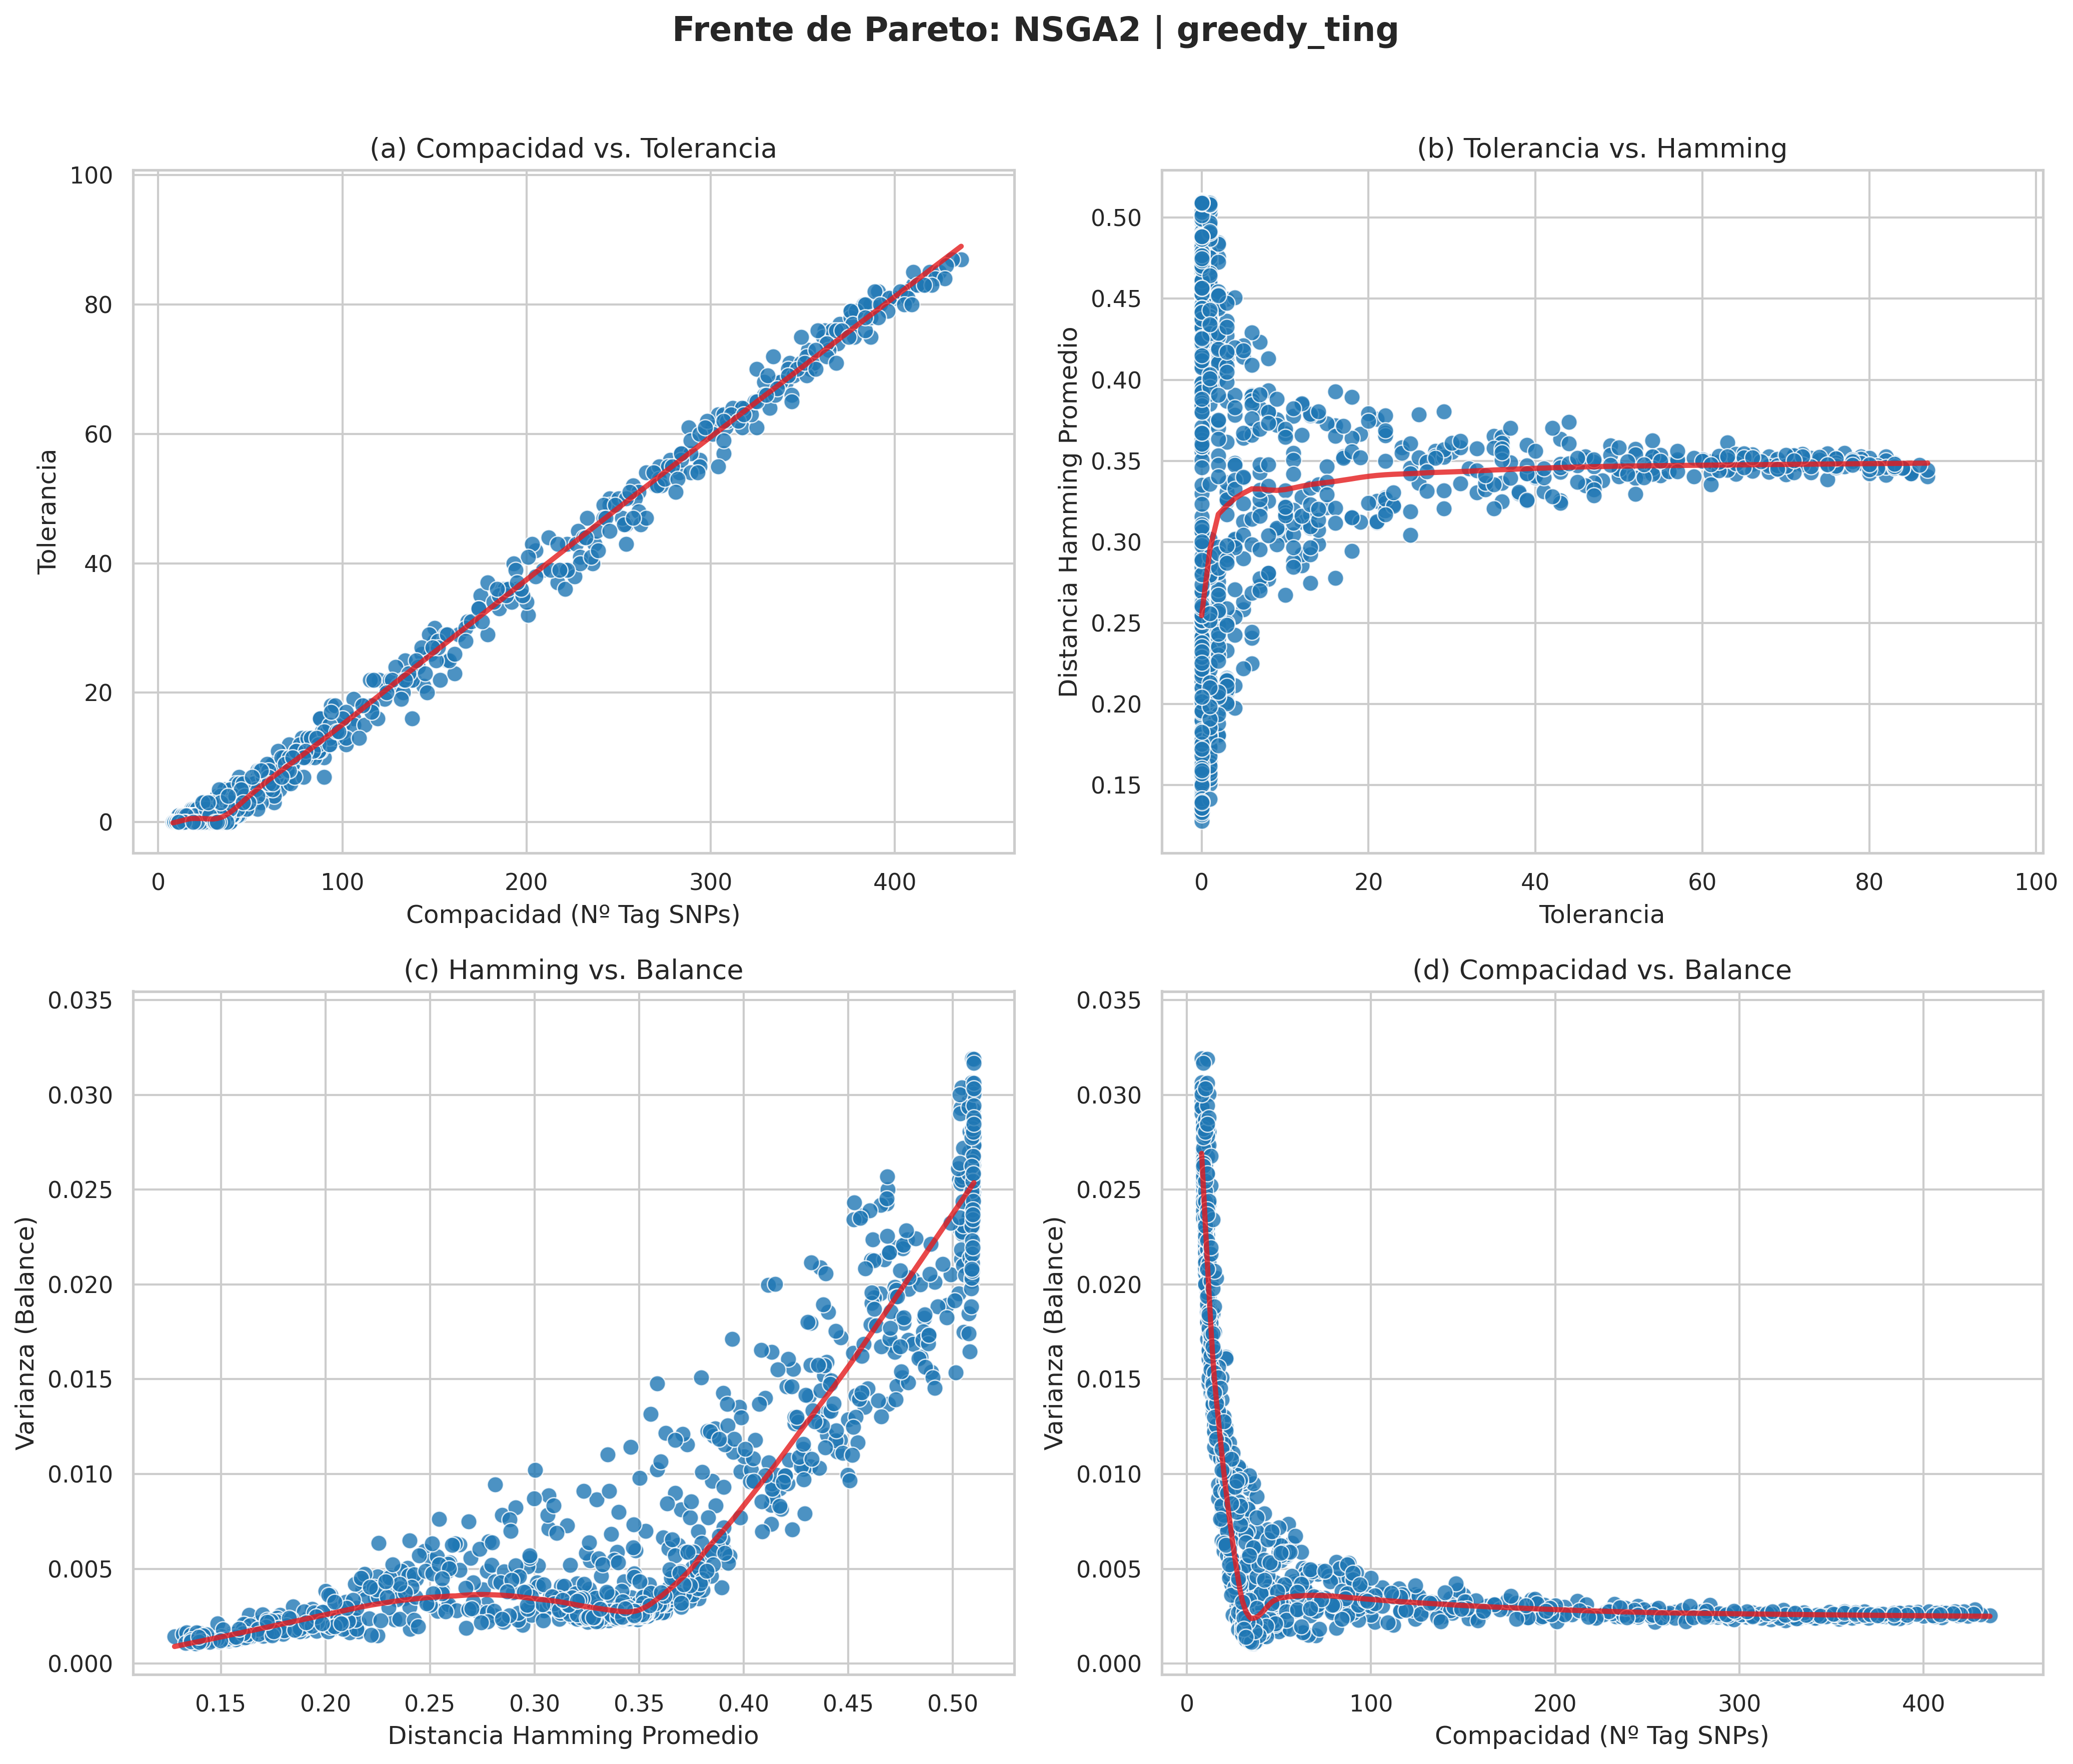
\includegraphics[width=\linewidth]{analisis_assets/20260430T183144/2_comparativa/1_frentes/frentes_pareto/frentes_pareto_nsga2_greedy_ting_full.png} & 
\includegraphics[width=\linewidth]{analisis_assets/20260430T183144/2_comparativa/1_frentes/frentes_pareto/frentes_pareto_nsga2_greedy_hybrid_full.png} \\
        \textbf{NSGA-III} & 
\includegraphics[width=\linewidth]{analisis_assets/20260430T183144/2_comparativa/1_frentes/frentes_pareto/frentes_pareto_nsga3_random_sparse_full.png} & 
\includegraphics[width=\linewidth]{analisis_assets/20260430T183144/2_comparativa/1_frentes/frentes_pareto/frentes_pareto_nsga3_random_dense_full.png} & 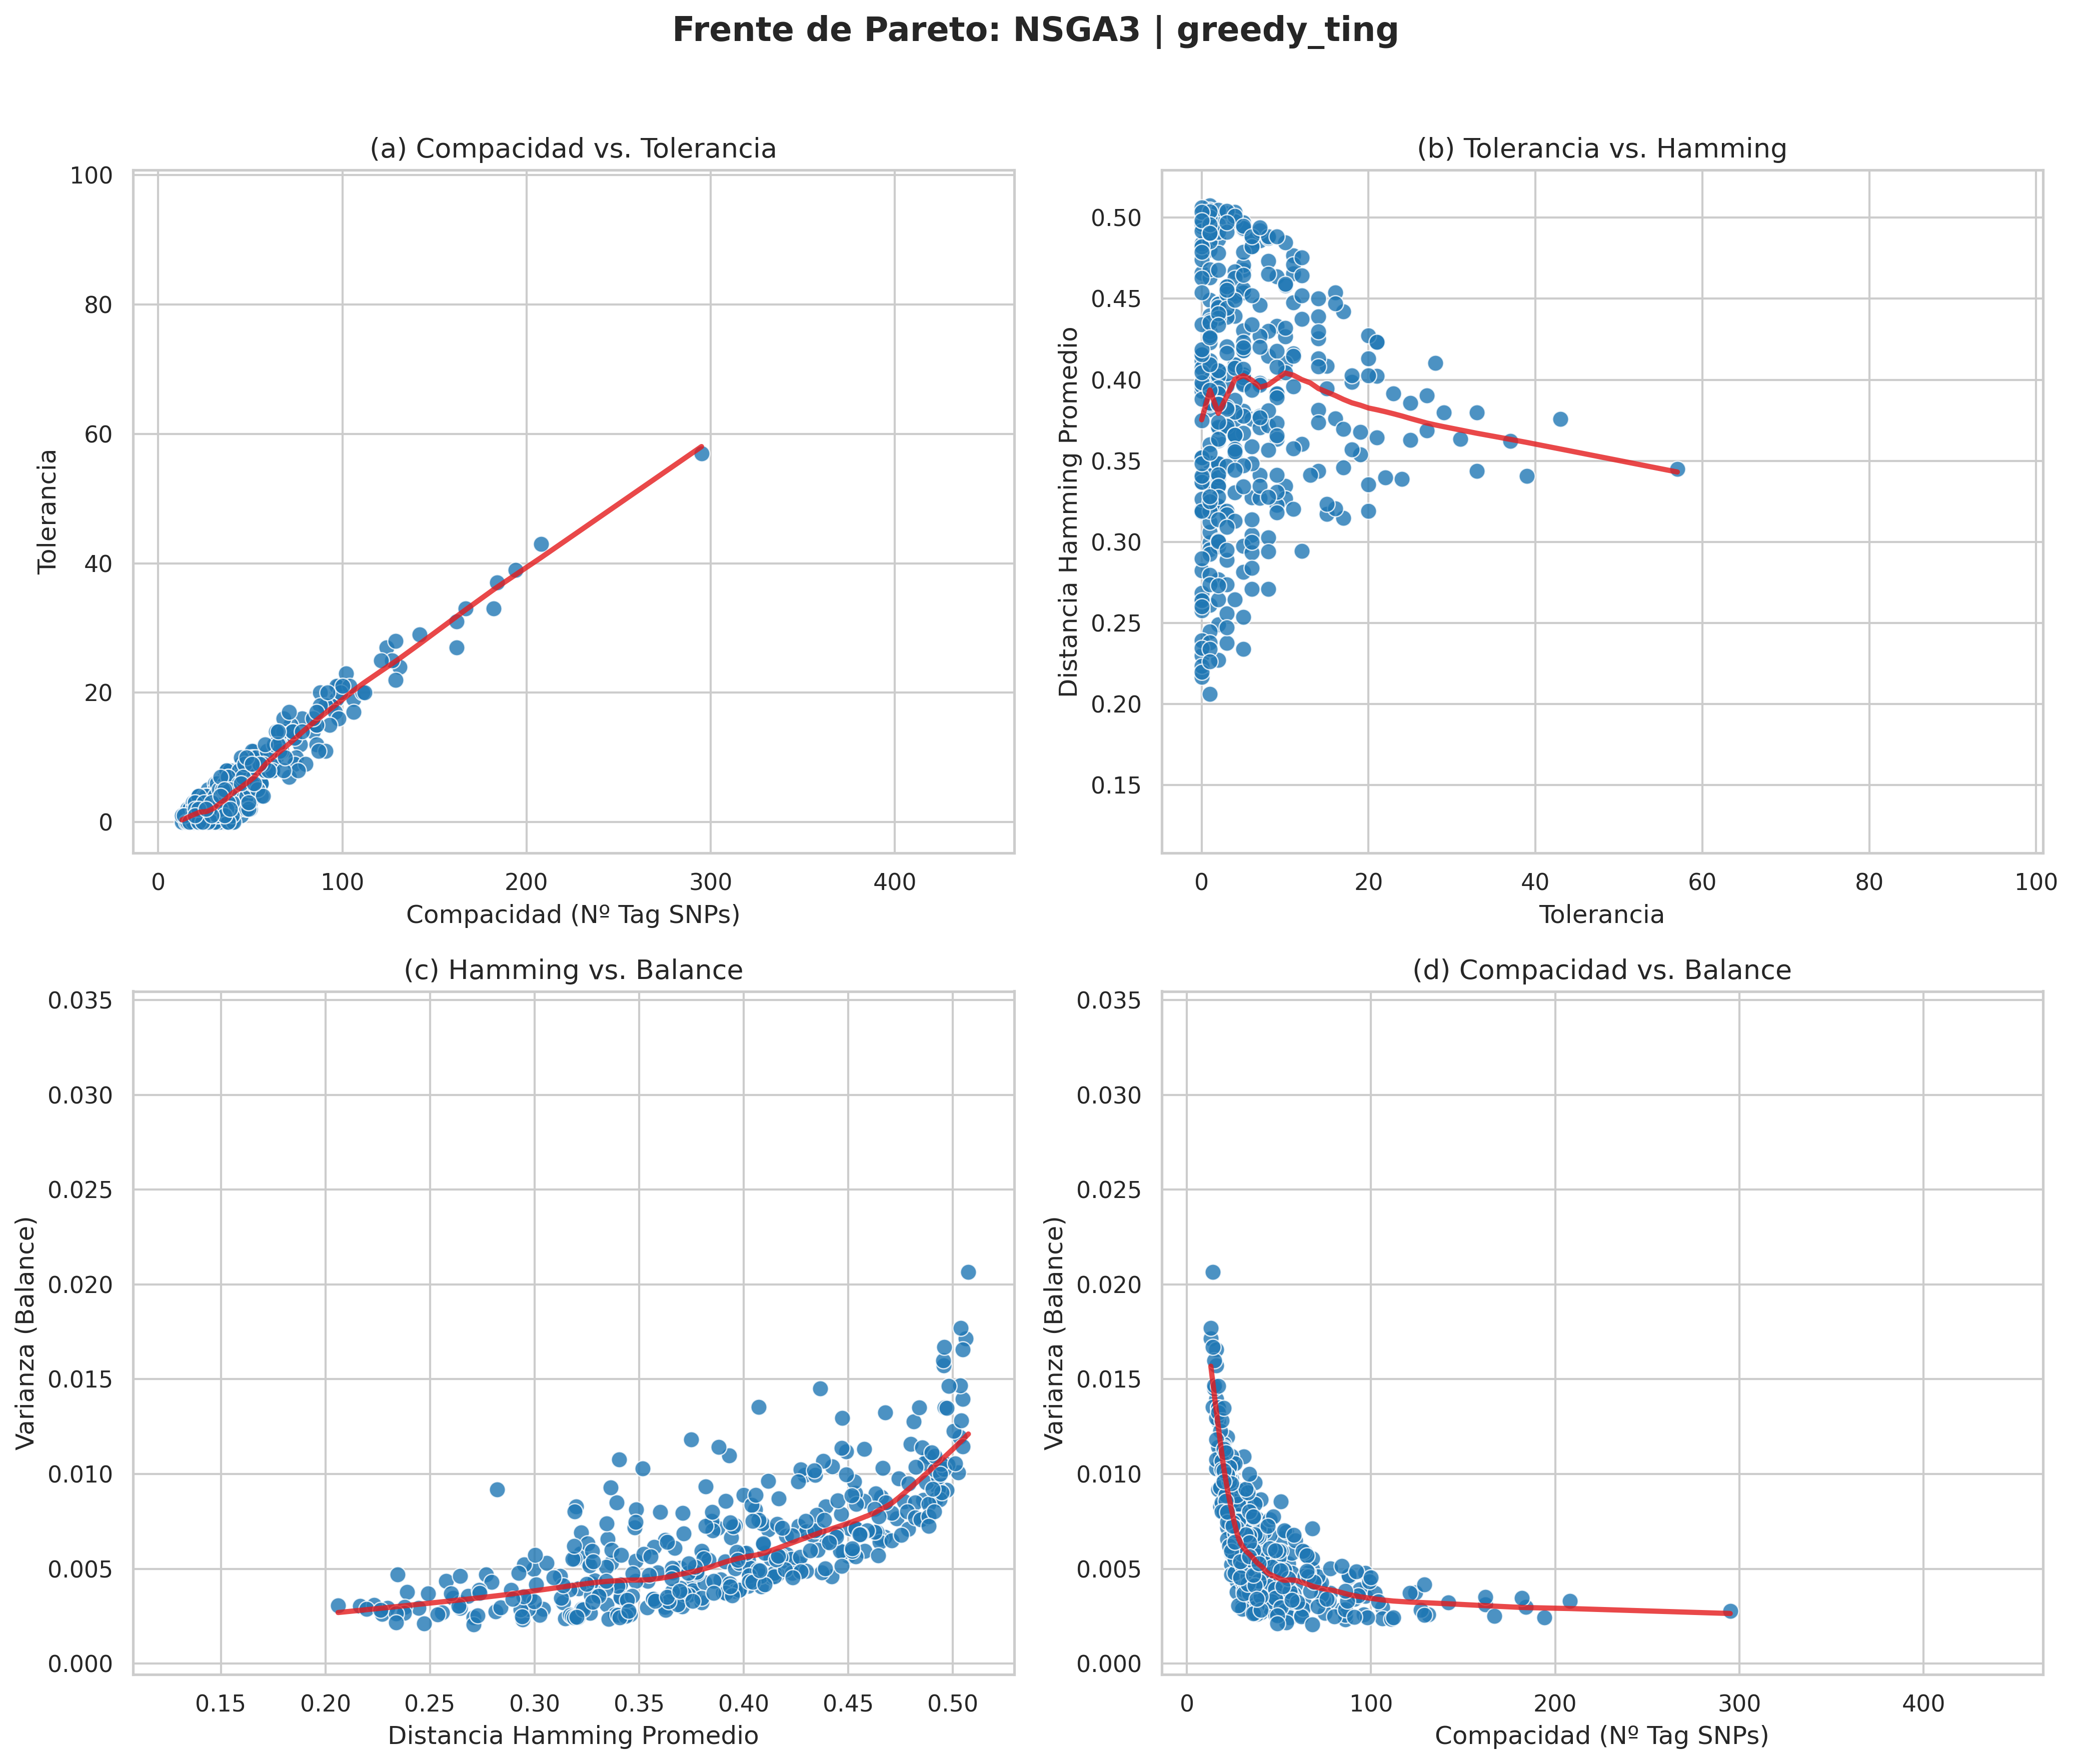
\includegraphics[width=\linewidth]{analisis_assets/20260430T183144/2_comparativa/1_frentes/frentes_pareto/frentes_pareto_nsga3_greedy_ting_full.png} & 
\includegraphics[width=\linewidth]{analisis_assets/20260430T183144/2_comparativa/1_frentes/frentes_pareto/frentes_pareto_nsga3_greedy_hybrid_full.png} \\
        \textbf{SPEA2} & 
\includegraphics[width=\linewidth]{analisis_assets/20260430T183144/2_comparativa/1_frentes/frentes_pareto/frentes_pareto_spea2_random_sparse_full.png} & 
\includegraphics[width=\linewidth]{analisis_assets/20260430T183144/2_comparativa/1_frentes/frentes_pareto/frentes_pareto_spea2_random_dense_full.png} & 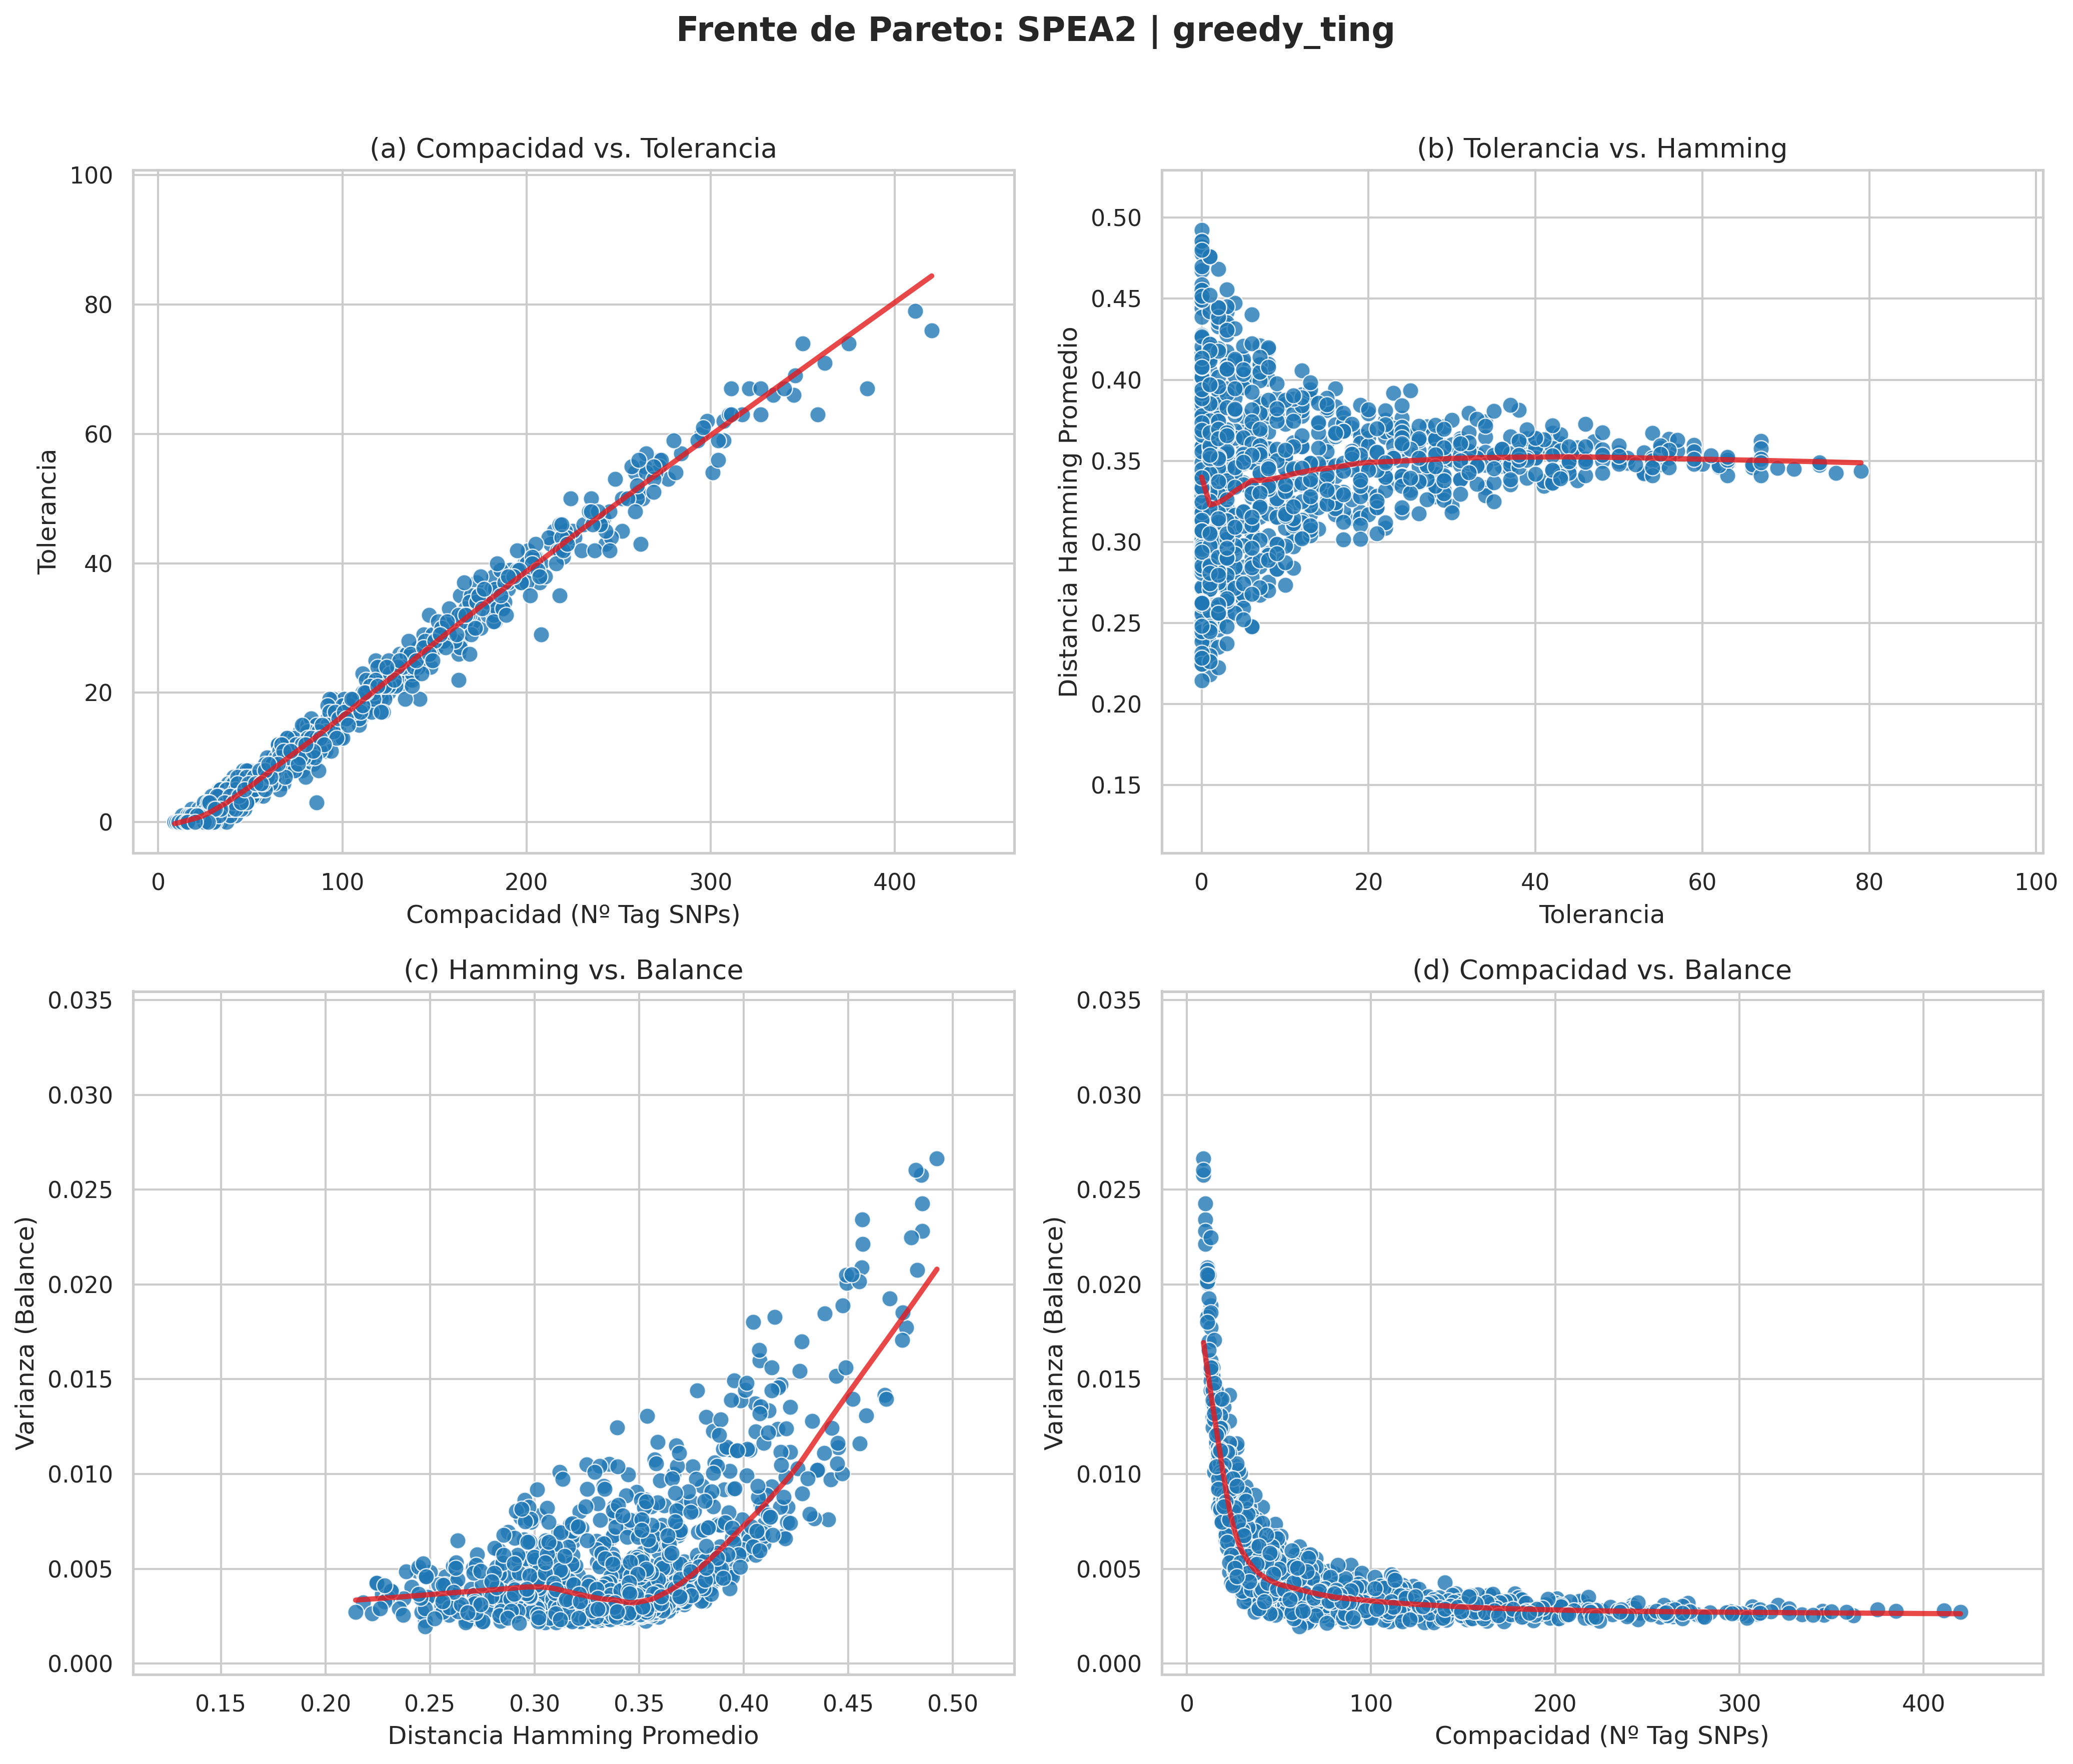
\includegraphics[width=\linewidth]{analisis_assets/20260430T183144/2_comparativa/1_frentes/frentes_pareto/frentes_pareto_spea2_greedy_ting_full.png} & 
\includegraphics[width=\linewidth]{analisis_assets/20260430T183144/2_comparativa/1_frentes/frentes_pareto/frentes_pareto_spea2_greedy_hybrid_full.png} \\
        \textbf{MOEA/D (PBI)} & 
\includegraphics[width=\linewidth]{analisis_assets/20260430T183144/2_comparativa/1_frentes/frentes_pareto/frentes_pareto_moead_pbi_random_sparse_full.png} & 
\includegraphics[width=\linewidth]{analisis_assets/20260430T183144/2_comparativa/1_frentes/frentes_pareto/frentes_pareto_moead_pbi_random_dense_full.png} & 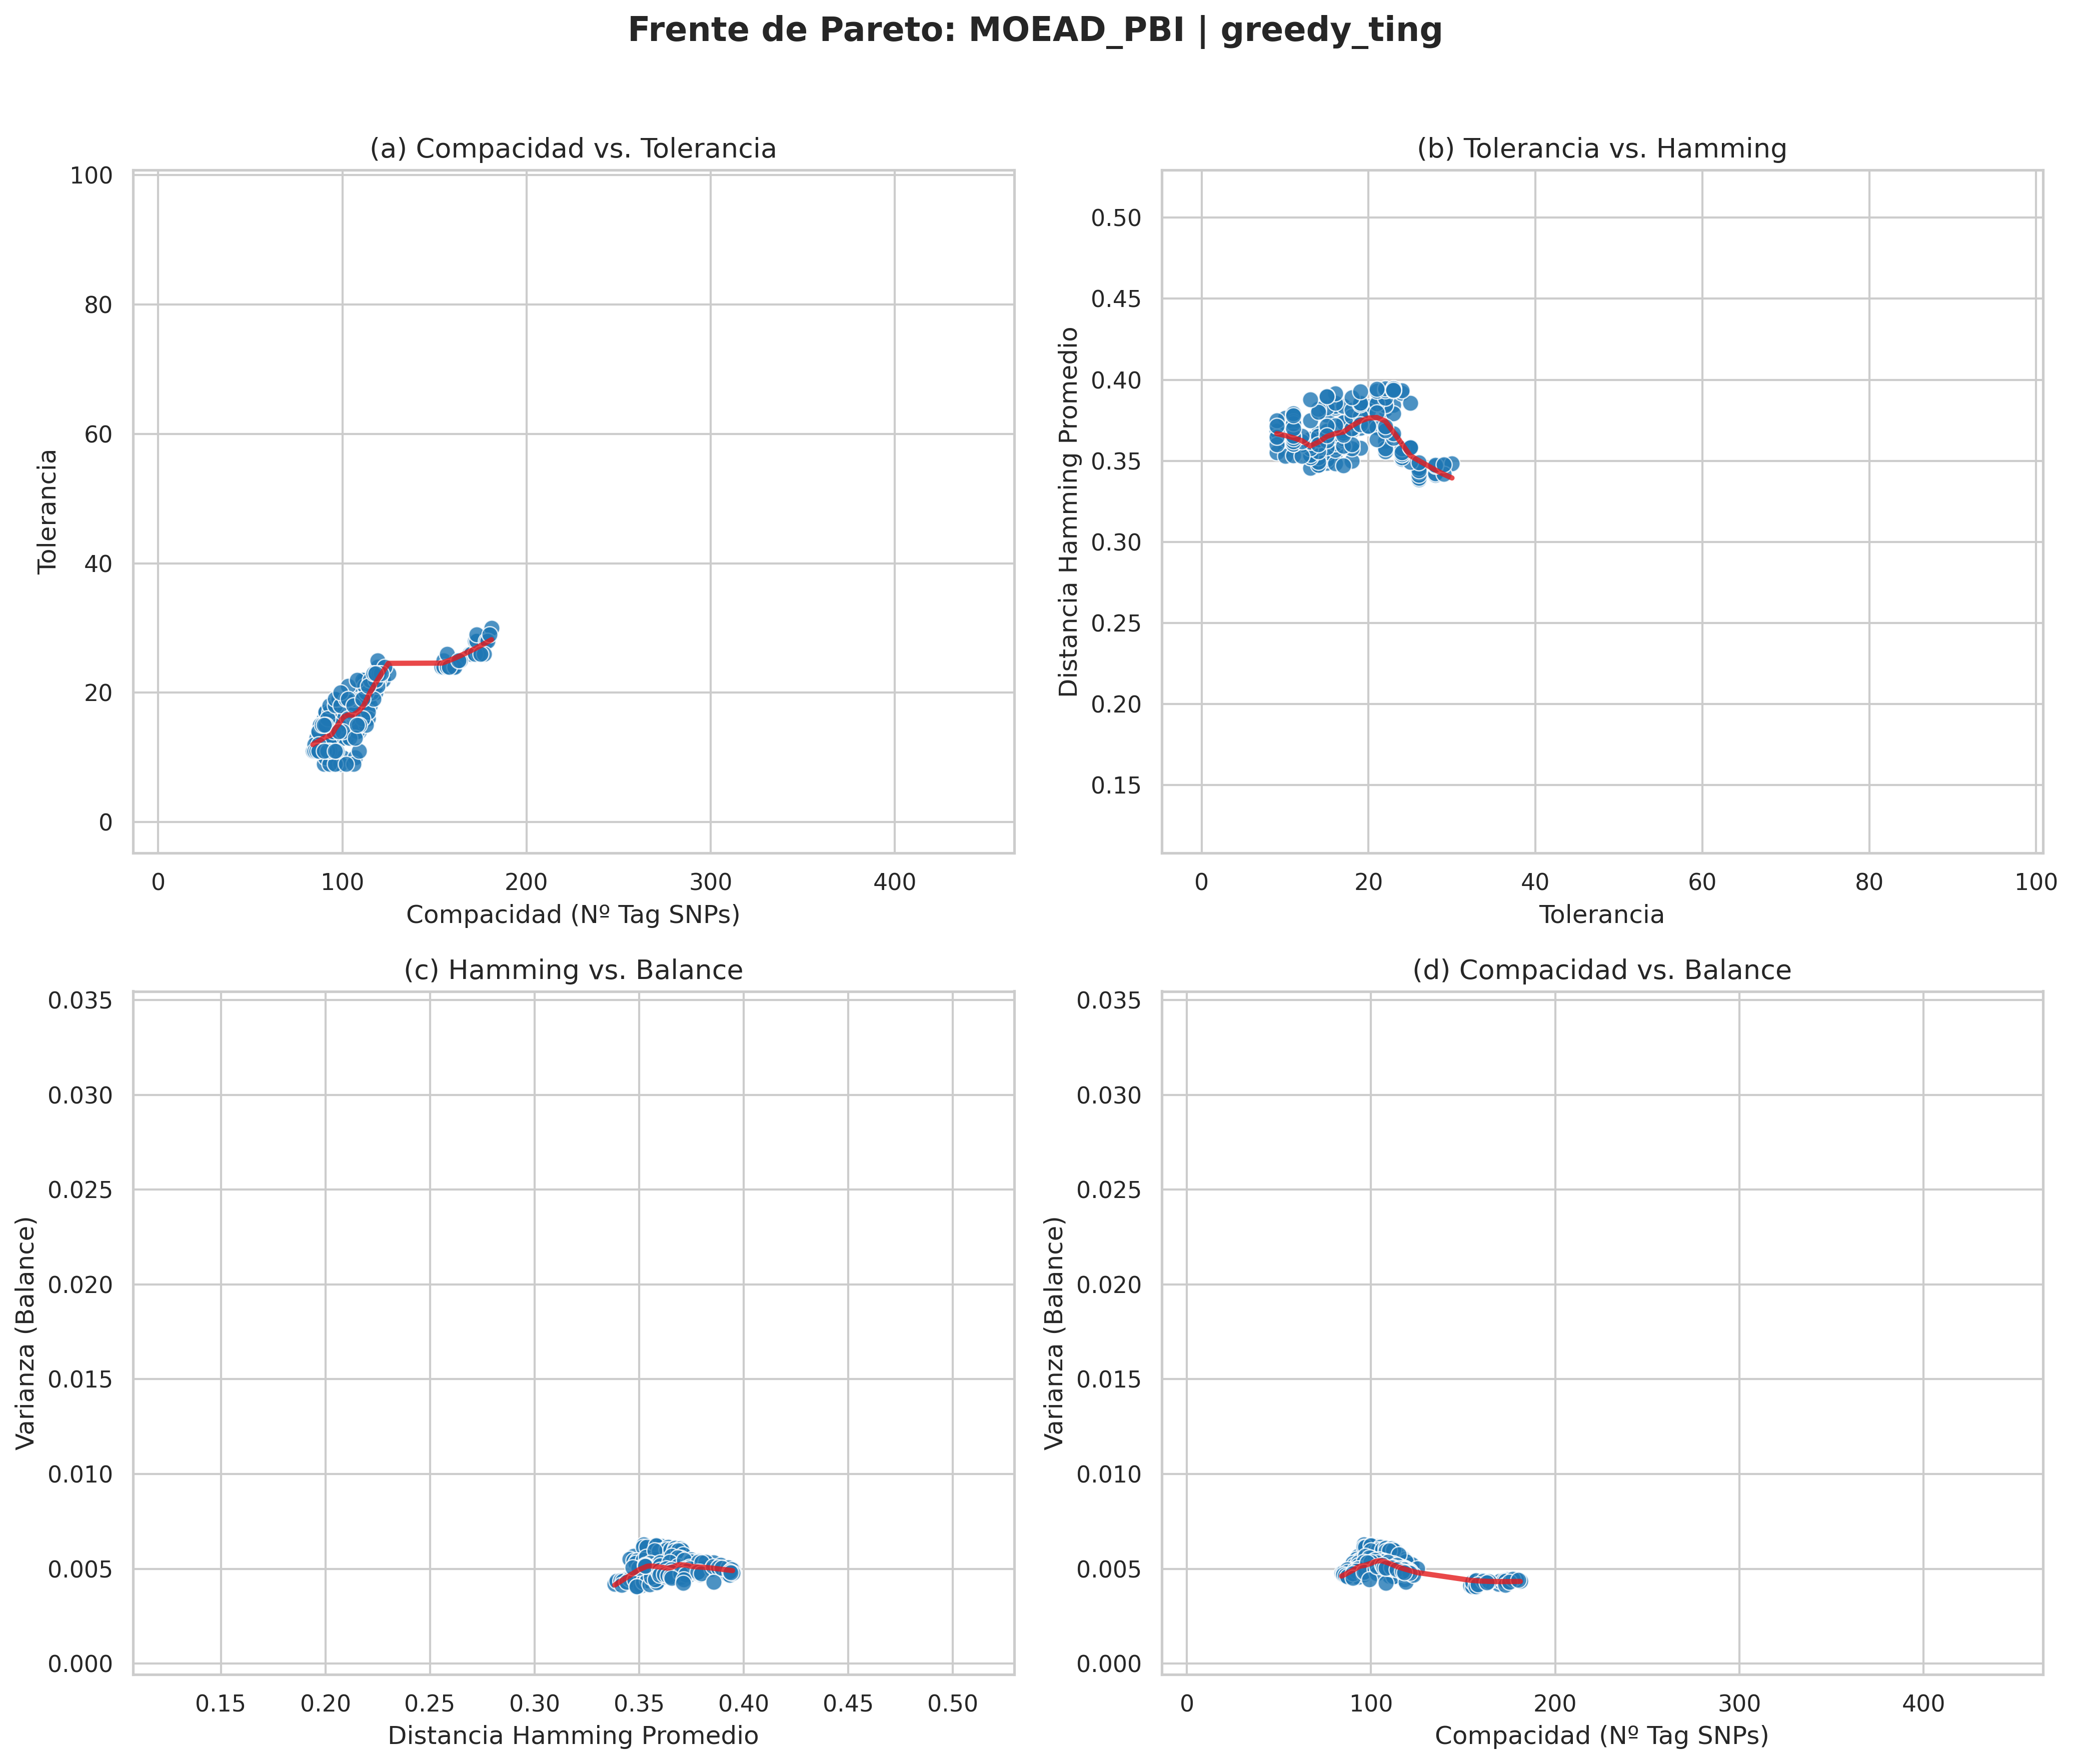
\includegraphics[width=\linewidth]{analisis_assets/20260430T183144/2_comparativa/1_frentes/frentes_pareto/frentes_pareto_moead_pbi_greedy_ting_full.png} & 
\includegraphics[width=\linewidth]{analisis_assets/20260430T183144/2_comparativa/1_frentes/frentes_pareto/frentes_pareto_moead_pbi_greedy_hybrid_full.png} \\
        \textbf{MOEA/D (TCHE)} & 
\includegraphics[width=\linewidth]{analisis_assets/20260430T183144/2_comparativa/1_frentes/frentes_pareto/frentes_pareto_moead_tche_random_sparse_full.png} & 
\includegraphics[width=\linewidth]{analisis_assets/20260430T183144/2_comparativa/1_frentes/frentes_pareto/frentes_pareto_moead_tche_random_dense_full.png} & 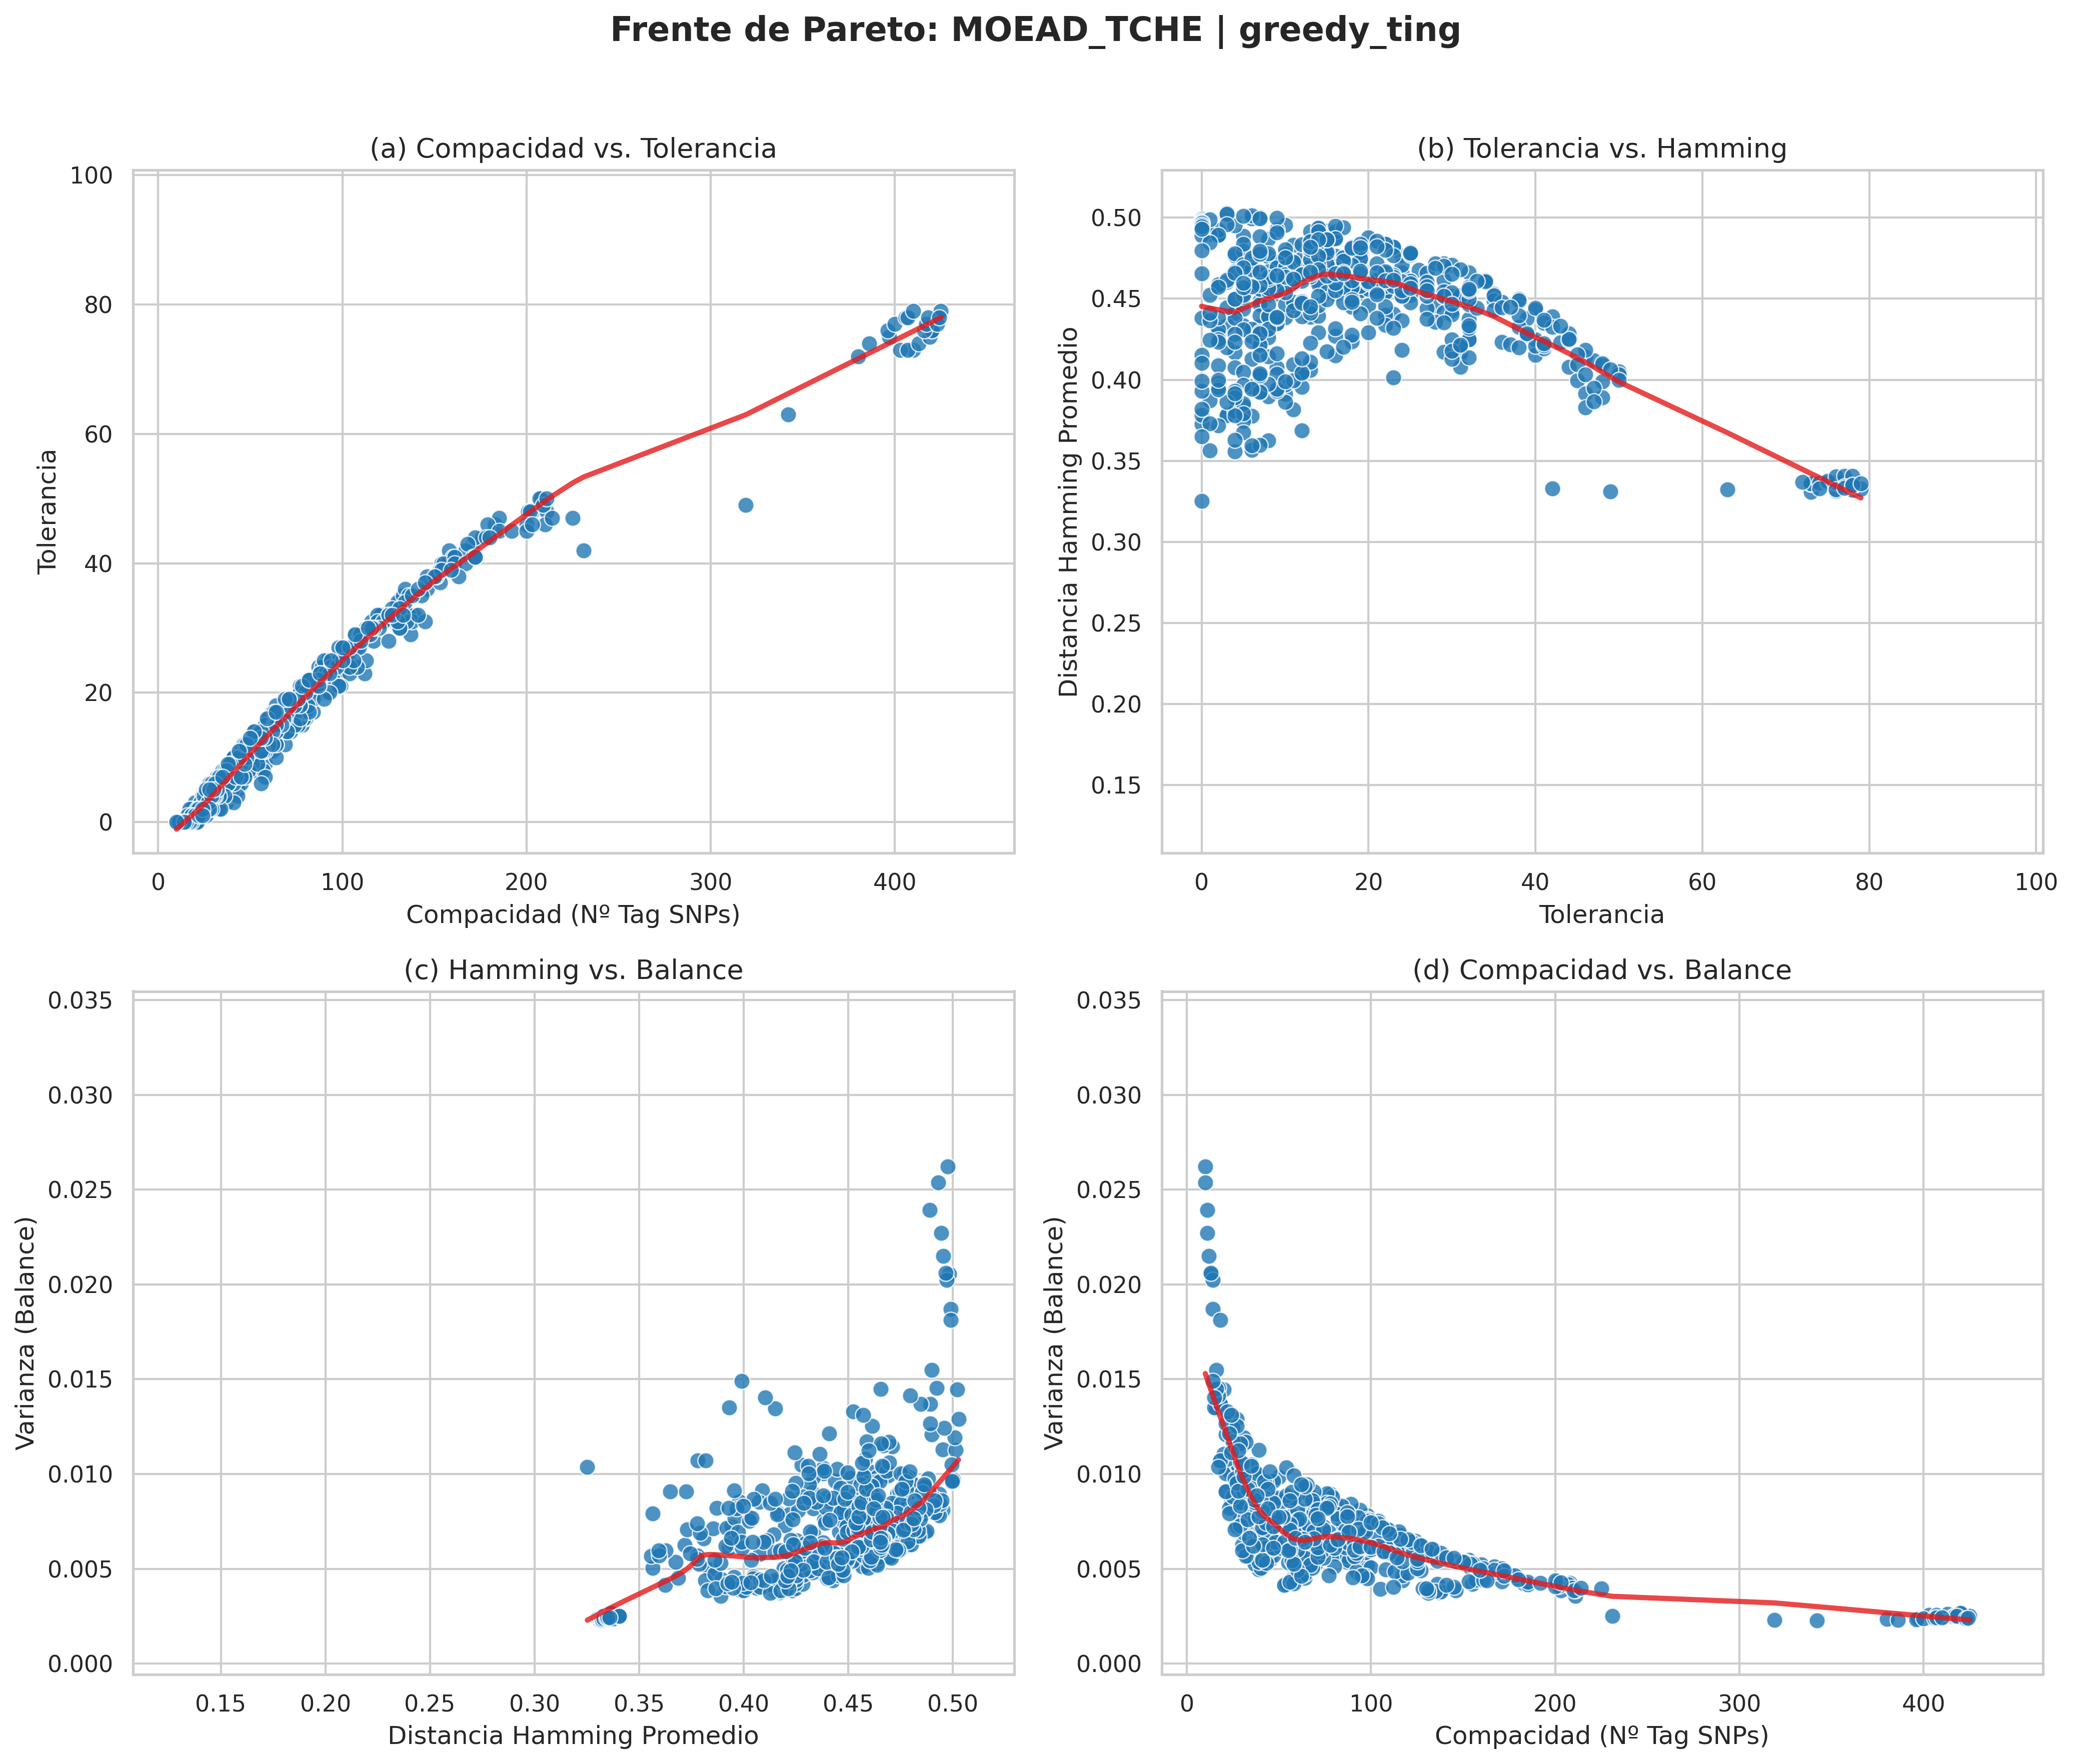
\includegraphics[width=\linewidth]{analisis_assets/20260430T183144/2_comparativa/1_frentes/frentes_pareto/frentes_pareto_moead_tche_greedy_ting_full.png} & 
\includegraphics[width=\linewidth]{analisis_assets/20260430T183144/2_comparativa/1_frentes/frentes_pareto/frentes_pareto_moead_tche_greedy_hybrid_full.png} \\
        \textbf{MOEA/D (WS)} & 
\includegraphics[width=\linewidth]{analisis_assets/20260430T183144/2_comparativa/1_frentes/frentes_pareto/frentes_pareto_moead_ws_random_sparse_full.png} & 
\includegraphics[width=\linewidth]{analisis_assets/20260430T183144/2_comparativa/1_frentes/frentes_pareto/frentes_pareto_moead_ws_random_dense_full.png} & 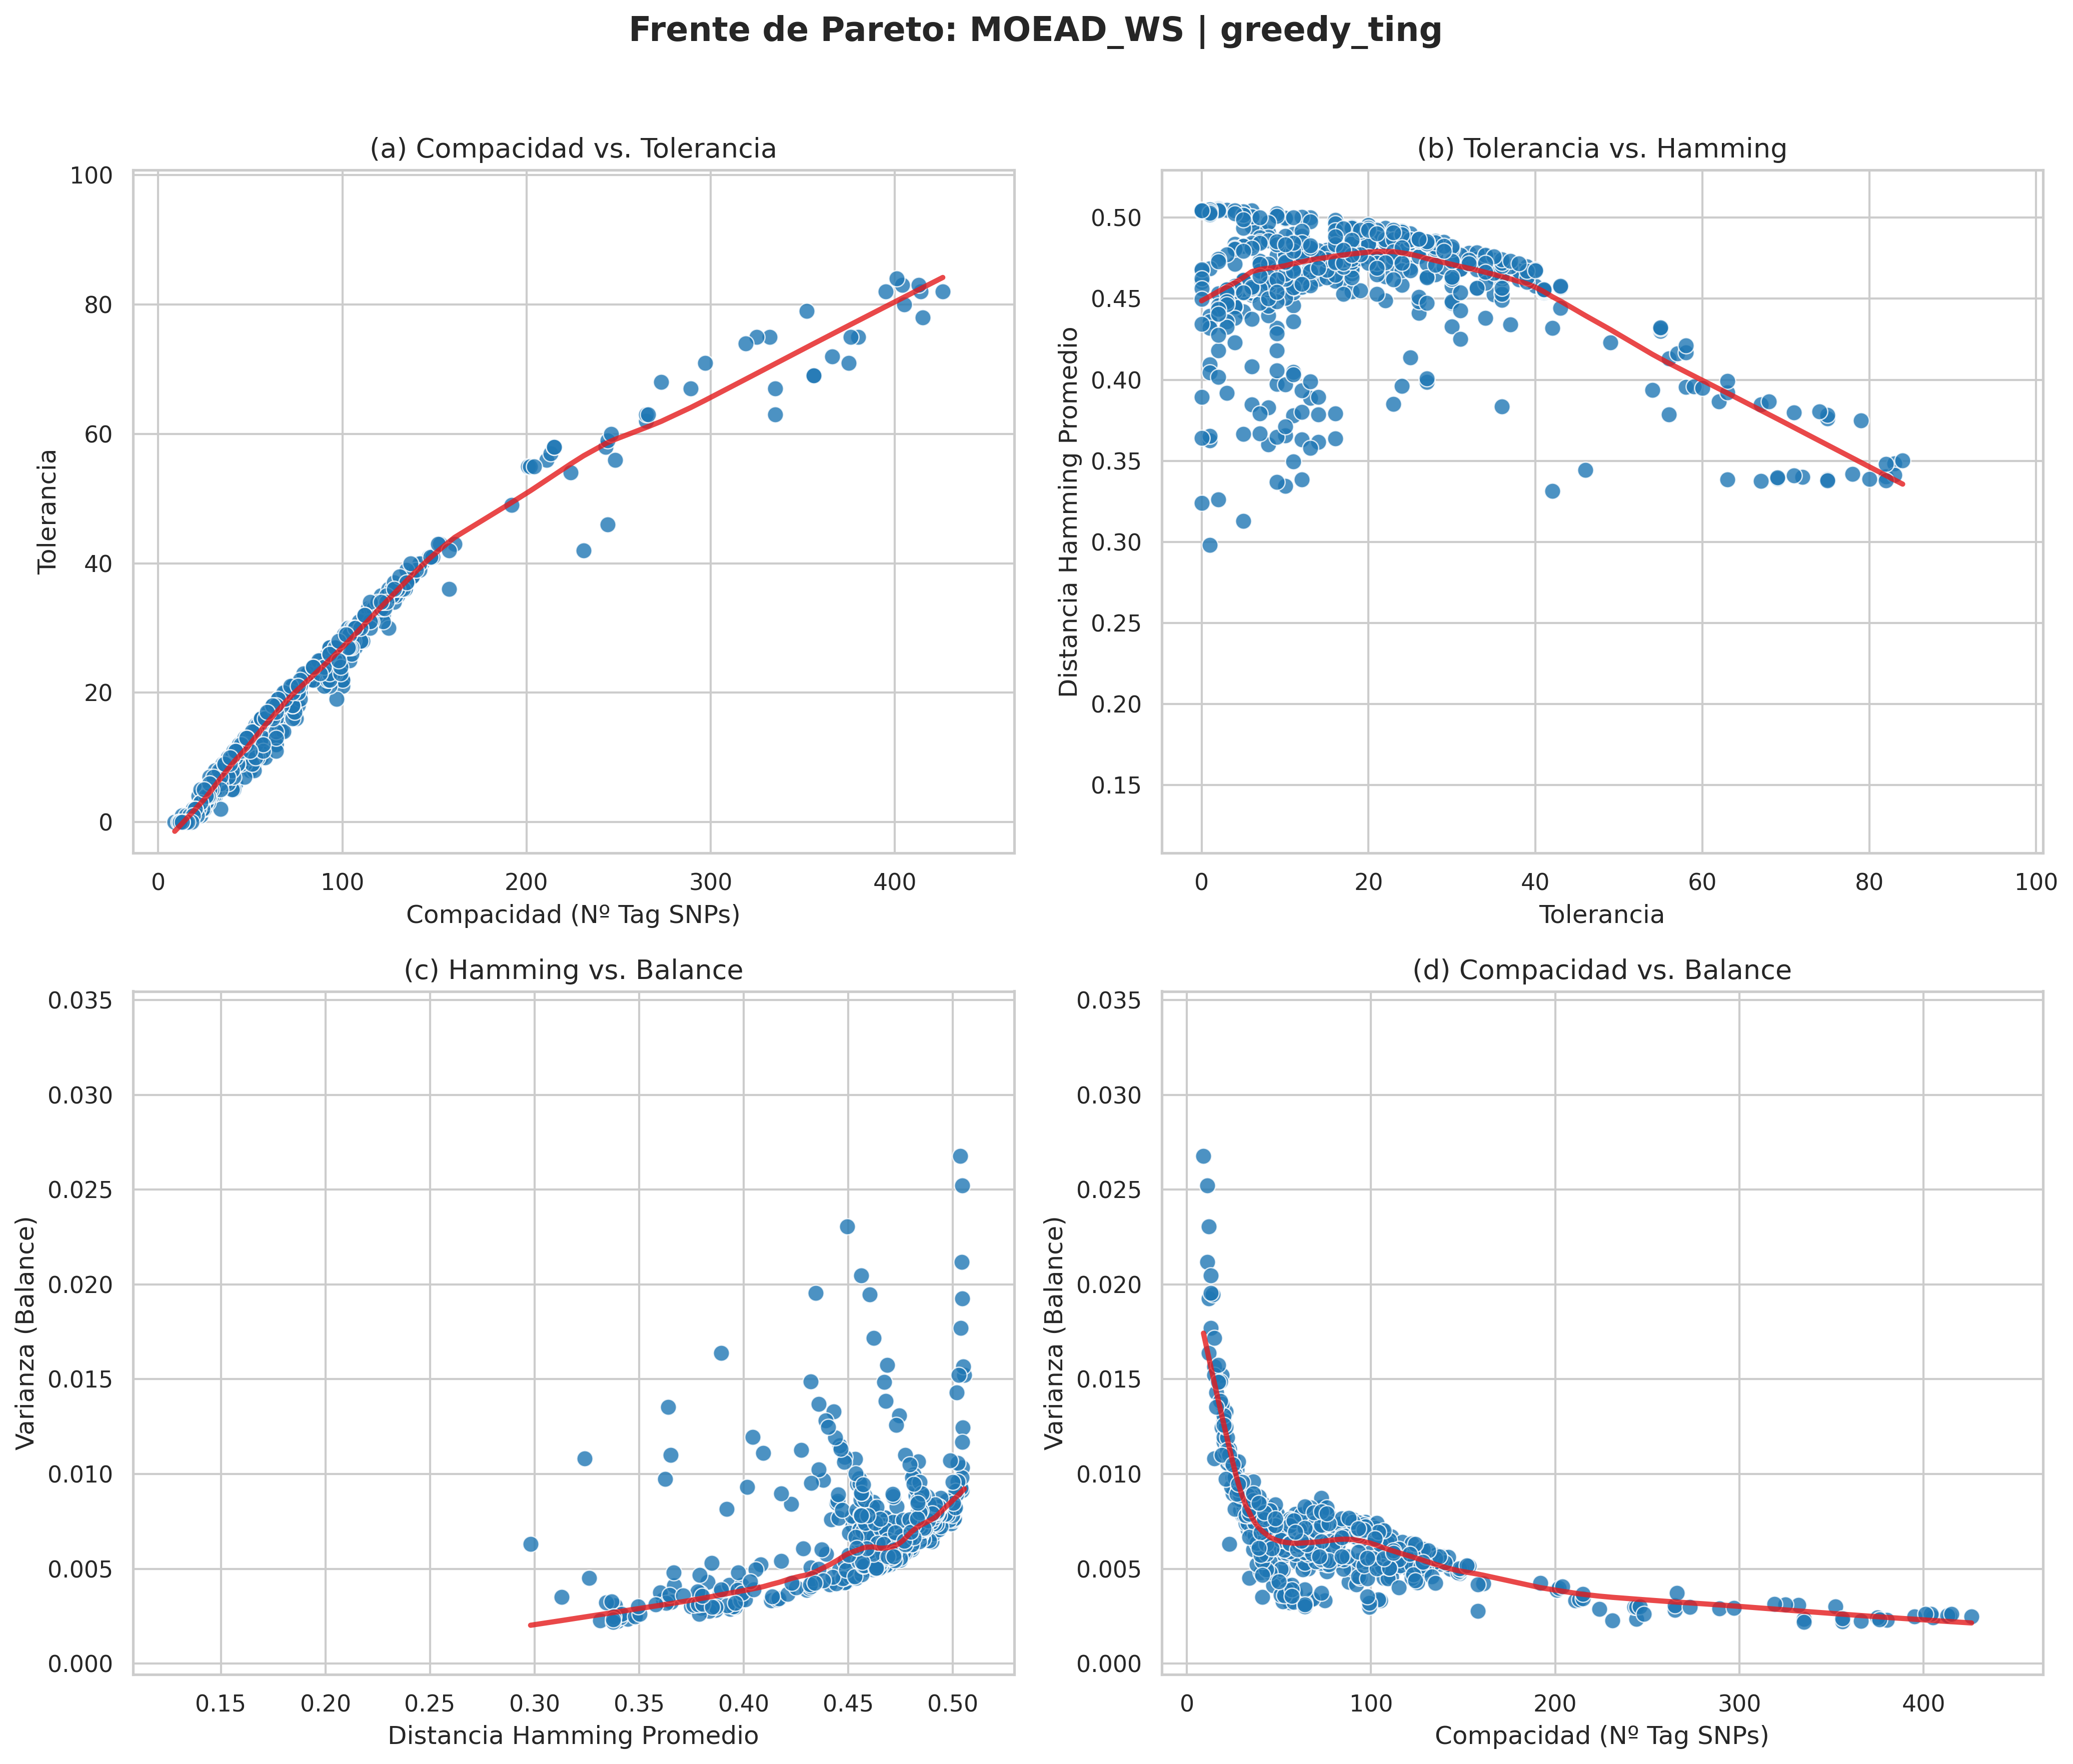
\includegraphics[width=\linewidth]{analisis_assets/20260430T183144/2_comparativa/1_frentes/frentes_pareto/frentes_pareto_moead_ws_greedy_ting_full.png} & 
\includegraphics[width=\linewidth]{analisis_assets/20260430T183144/2_comparativa/1_frentes/frentes_pareto/frentes_pareto_moead_ws_greedy_hybrid_full.png} \\
        \bottomrule
    \end{tabular}
    \caption{Galería de Frentes de Pareto (B)}
\end{table}

\subsubsection{Convergencia Progresiva (B)}
\begin{figure}[H]
    \centering
    \begin{subfigure}[b]{0.40\textwidth}
        
\includegraphics[width=\textwidth]{analisis_assets/20260430T183144/2_comparativa/2_metricas_convergencia/convergencia_range_full.png}
        \caption{Range}
    \end{subfigure}
    \hfill
    \begin{subfigure}[b]{0.40\textwidth}
        
\includegraphics[width=\textwidth]{analisis_assets/20260430T183144/2_comparativa/2_metricas_convergencia/convergencia_summin_full.png}
        \caption{SumMin}
    \end{subfigure}

    \vspace{0.3cm}

    \begin{subfigure}[b]{0.40\textwidth}
        
\includegraphics[width=\textwidth]{analisis_assets/20260430T183144/2_comparativa/2_metricas_convergencia/convergencia_minsum_full.png}
        \caption{MinSum}
    \end{subfigure}
    \hfill
    \begin{subfigure}[b]{0.40\textwidth}
        
\includegraphics[width=\textwidth]{analisis_assets/20260430T183144/2_comparativa/2_metricas_convergencia/convergencia_avghammingdistance_full.png}
        \caption{Avg Hamming}
    \end{subfigure}

    \vspace{0.3cm}

    \begin{subfigure}[b]{0.40\textwidth}
        
\includegraphics[width=\textwidth]{analisis_assets/20260430T183144/2_comparativa/2_metricas_convergencia/convergencia_hypervolume_full.png}
        \caption{Hypervolume}
    \end{subfigure}
    \caption{Galería de Convergencia (Ejecución B)}
\end{figure}

\subsubsection{Top 10 por Métrica (B)}
% Tables for Experiment B
\subparagraph{Top 10: Range ($\uparrow$)}
\begin{table}[H]
    \centering
    \begin{tabular}{cllc}
        \toprule
        Pos & Algoritmo & Inicialización & Valor ($\mu \pm \sigma$) \\
        \midrule
        1 & NSGA2 & greedy\_ting & 2.2075 $\pm$ 0.0961 \\
        2 & NSGA2 & greedy\_hybrid & 2.0661 $\pm$ 0.0632 \\
        3 & SPEA2 & greedy\_ting & 1.8136 $\pm$ 0.0559 \\
        4 & SPEA2 & greedy\_hybrid & 1.7874 $\pm$ 0.0344 \\
        5 & NSGA2 & random\_sparse & 1.7767 $\pm$ 0.0474 \\
        6 & SPEA2 & random\_sparse & 1.6623 $\pm$ 0.1173 \\
        7 & MOEAD\_TCHE & greedy\_hybrid & 1.5798 $\pm$ 0.1056 \\
        8 & MOEAD\_WS & greedy\_hybrid & 1.5506 $\pm$ 0.1351 \\
        9 & NSGA3 & greedy\_ting & 1.5457 $\pm$ 0.0929 \\
        10 & NSGA3 & greedy\_hybrid & 1.4686 $\pm$ 0.0787 \\
        \bottomrule
    \end{tabular}
    \caption{Top 10 para Range en Ejecución B (Promedio +- Desv. Est.).}
\end{table}

\subparagraph{Top 10: SumMin ($\downarrow$)}
\begin{table}[H]
    \centering
    \begin{tabular}{cllc}
        \toprule
        Pos & Algoritmo & Inicialización & Valor ($\mu \pm \sigma$) \\
        \midrule
        1 & NSGA2 & greedy\_ting & 0.1251 $\pm$ 0.0007 \\
        2 & NSGA2 & greedy\_hybrid & 0.1272 $\pm$ 0.0015 \\
        3 & MOEAD\_WS & greedy\_hybrid & 0.1398 $\pm$ 0.0059 \\
        4 & MOEAD\_TCHE & greedy\_hybrid & 0.1428 $\pm$ 0.0042 \\
        5 & SPEA2 & greedy\_hybrid & 0.1461 $\pm$ 0.0094 \\
        6 & SPEA2 & greedy\_ting & 0.1490 $\pm$ 0.0108 \\
        7 & MOEAD\_WS & greedy\_ting & 0.1498 $\pm$ 0.0132 \\
        8 & NSGA2 & random\_sparse & 0.1528 $\pm$ 0.0023 \\
        9 & MOEAD\_TCHE & greedy\_ting & 0.1574 $\pm$ 0.0219 \\
        10 & NSGA3 & greedy\_ting & 0.1580 $\pm$ 0.0087 \\
        \bottomrule
    \end{tabular}
    \caption{Top 10 para SumMin en Ejecución B (Promedio +- Desv. Est.).}
\end{table}

\subparagraph{Top 10: MinSum ($\downarrow$)}
\begin{table}[H]
    \centering
    \begin{tabular}{cllc}
        \toprule
        Pos & Algoritmo & Inicialización & Valor ($\mu \pm \sigma$) \\
        \midrule
        1 & MOEAD\_WS & greedy\_hybrid & 0.2718 $\pm$ 0.0023 \\
        2 & MOEAD\_WS & greedy\_ting & 0.2726 $\pm$ 0.0047 \\
        3 & MOEAD\_TCHE & greedy\_hybrid & 0.2804 $\pm$ 0.0047 \\
        4 & MOEAD\_TCHE & greedy\_ting & 0.2875 $\pm$ 0.0126 \\
        5 & MOEAD\_TCHE & random\_sparse & 0.2901 $\pm$ 0.0063 \\
        6 & MOEAD\_WS & random\_sparse & 0.2922 $\pm$ 0.0053 \\
        7 & NSGA3 & greedy\_hybrid & 0.2928 $\pm$ 0.0041 \\
        8 & NSGA3 & greedy\_ting & 0.2947 $\pm$ 0.0034 \\
        9 & NSGA3 & random\_sparse & 0.2972 $\pm$ 0.0108 \\
        10 & MOEAD\_PBI & random\_sparse & 0.3138 $\pm$ 0.0135 \\
        \bottomrule
    \end{tabular}
    \caption{Top 10 para MinSum en Ejecución B (Promedio +- Desv. Est.).}
\end{table}

\subparagraph{Top 10: MaxToleranceRate ($\uparrow$)}
\begin{table}[H]
    \centering
    \begin{tabular}{cllc}
        \toprule
        Pos & Algoritmo & Inicialización & Valor ($\mu \pm \sigma$) \\
        \midrule
        1 & MOEAD\_WS & greedy\_ting & 0.2919 $\pm$ 0.0030 \\
        2 & MOEAD\_WS & greedy\_hybrid & 0.2825 $\pm$ 0.0031 \\
        3 & MOEAD\_TCHE & greedy\_ting & 0.2738 $\pm$ 0.0068 \\
        4 & NSGA3 & random\_dense & 0.2697 $\pm$ 0.0032 \\
        5 & MOEAD\_TCHE & greedy\_hybrid & 0.2649 $\pm$ 0.0040 \\
        6 & MOEAD\_TCHE & random\_sparse & 0.2580 $\pm$ 0.0069 \\
        7 & MOEAD\_WS & random\_sparse & 0.2542 $\pm$ 0.0058 \\
        8 & NSGA2 & random\_dense & 0.2523 $\pm$ 0.0069 \\
        9 & SPEA2 & random\_dense & 0.2430 $\pm$ 0.0077 \\
        10 & MOEAD\_PBI & random\_sparse & 0.2291 $\pm$ 0.0124 \\
        \bottomrule
    \end{tabular}
    \caption{Top 10 para MaxToleranceRate en Ejecución B (Promedio +- Desv. Est.).}
\end{table}

\subparagraph{Top 10: AvgToleranceRate ($\uparrow$)}
\begin{table}[H]
    \centering
    \begin{tabular}{cllc}
        \toprule
        Pos & Algoritmo & Inicialización & Valor ($\mu \pm \sigma$) \\
        \midrule
        1 & NSGA3 & random\_dense & 0.2389 $\pm$ 0.0043 \\
        2 & MOEAD\_WS & greedy\_ting & 0.2245 $\pm$ 0.0075 \\
        3 & NSGA2 & random\_dense & 0.2124 $\pm$ 0.0061 \\
        4 & MOEAD\_WS & greedy\_hybrid & 0.2122 $\pm$ 0.0031 \\
        5 & MOEAD\_WS & random\_sparse & 0.2095 $\pm$ 0.0080 \\
        6 & MOEAD\_PBI & random\_sparse & 0.2093 $\pm$ 0.0125 \\
        7 & MOEAD\_WS & random\_dense & 0.2051 $\pm$ 0.0081 \\
        8 & MOEAD\_TCHE & greedy\_ting & 0.2015 $\pm$ 0.0068 \\
        9 & MOEAD\_TCHE & random\_sparse & 0.2012 $\pm$ 0.0024 \\
        10 & MOEAD\_TCHE & random\_dense & 0.1993 $\pm$ 0.0070 \\
        \bottomrule
    \end{tabular}
    \caption{Top 10 para AvgToleranceRate en Ejecución B (Promedio +- Desv. Est.).}
\end{table}

\subparagraph{Top 10: AvgHammingDistance ($\uparrow$)}
\begin{table}[H]
    \centering
    \begin{tabular}{cllc}
        \toprule
        Pos & Algoritmo & Inicialización & Valor ($\mu \pm \sigma$) \\
        \midrule
        1 & MOEAD\_WS & greedy\_hybrid & 0.4631 $\pm$ 0.0022 \\
        2 & MOEAD\_WS & greedy\_ting & 0.4551 $\pm$ 0.0066 \\
        3 & MOEAD\_TCHE & greedy\_hybrid & 0.4500 $\pm$ 0.0014 \\
        4 & MOEAD\_TCHE & random\_sparse & 0.4455 $\pm$ 0.0082 \\
        5 & MOEAD\_TCHE & greedy\_ting & 0.4405 $\pm$ 0.0121 \\
        6 & MOEAD\_WS & random\_sparse & 0.4386 $\pm$ 0.0088 \\
        7 & MOEAD\_PBI & random\_sparse & 0.4169 $\pm$ 0.0128 \\
        8 & MOEAD\_PBI & greedy\_hybrid & 0.4107 $\pm$ 0.0100 \\
        9 & NSGA3 & greedy\_hybrid & 0.4076 $\pm$ 0.0111 \\
        10 & NSGA3 & random\_sparse & 0.4061 $\pm$ 0.0092 \\
        \bottomrule
    \end{tabular}
    \caption{Top 10 para AvgHammingDistance en Ejecución B (Promedio +- Desv. Est.).}
\end{table}

\subparagraph{Top 10: Hypervolume ($\uparrow$)}
\begin{table}[H]
    \centering
    \begin{tabular}{cllc}
        \toprule
        Pos & Algoritmo & Inicialización & Valor ($\mu \pm \sigma$) \\
        \midrule
        1 & MOEAD\_WS & greedy\_hybrid & 1.2607 $\pm$ 0.0047 \\
        2 & MOEAD\_WS & greedy\_ting & 1.2509 $\pm$ 0.0111 \\
        3 & MOEAD\_TCHE & greedy\_hybrid & 1.2503 $\pm$ 0.0028 \\
        4 & NSGA3 & greedy\_ting & 1.2414 $\pm$ 0.0074 \\
        5 & NSGA3 & greedy\_hybrid & 1.2412 $\pm$ 0.0073 \\
        6 & NSGA2 & greedy\_hybrid & 1.2401 $\pm$ 0.0046 \\
        7 & MOEAD\_TCHE & greedy\_ting & 1.2388 $\pm$ 0.0204 \\
        8 & NSGA2 & greedy\_ting & 1.2377 $\pm$ 0.0041 \\
        9 & SPEA2 & greedy\_hybrid & 1.2227 $\pm$ 0.0073 \\
        10 & SPEA2 & greedy\_ting & 1.2164 $\pm$ 0.0081 \\
        \bottomrule
    \end{tabular}
    \caption{Top 10 para Hypervolume en Ejecución B (Promedio +- Desv. Est.).}
\end{table}


\subsubsection{Validación Estadística (B)}
La validación estadística para el entorno invertido confirma las tendencias observadas en el entorno lineal, con una significancia aún más marcada en la diferenciación de métodos.

\begin{itemize}
    \item \textbf{Test de Friedman (Método):} p-valor de $3.4598 \times 10^{-7}$ (Significativo).
    \item \textbf{Test de Friedman (Algoritmo):} p-valor de $0.10120$ (No significativo).
    \item \textbf{Test de Friedman (Inicialización):} p-valor de $0.0070952$ (Significativo).
\end{itemize}

\begin{figure}[H]
    \centering
    \begin{subfigure}[b]{0.48\textwidth}
        
\includegraphics[width=\textwidth]{analisis_assets/20260430T183144/2_comparativa/4_rankings/estadistica/method/heatmap_nemenyi_full.png}
        \caption{Significancia Nemenyi (Algoritmo+Init)}
    \end{subfigure}
    \hfill
    \begin{subfigure}[b]{0.48\textwidth}
        
\includegraphics[width=\textwidth]{analisis_assets/20260430T183144/2_comparativa/4_rankings/estadistica/init/heatmap_nemenyi_init_full.png}
        \caption{Significancia Nemenyi (Inicialización)}
    \end{subfigure}
    \caption{Mapas de calor de significancia estadística para la Ejecución B. Las celdas en blanco o tonos claros indican pares de métodos sin diferencias significativas ($p > 0,05$).}
\end{figure}

\subsubsection{Análisis de Significancia (Nemenyi)}
En la Ejecución B, no se detecta una discriminación estadística robusta entre algoritmos, coherente con el p-valor de Friedman ($p=0,10120$). El mapa de significancia de Nemenyi muestra que una gran parte de las comparativas por pares resultan no significativas. Este fenómeno sugiere que la transformación recíproca de los objetivos genera un paisaje de búsqueda donde las diferencias intrínsecas de los algoritmos (basados en frentes vs. basados en descomposición) se atenúan, delegando una parte relevante del éxito de la optimización a la calidad de la población inicial. 

Al igual que en la Ejecución A, se plantea que un mayor número de ejecuciones independientes podría dotar al test de la potencia necesaria para identificar matices competitivos que la muestra actual no permite discriminar.

\subsubsection{Correlación de Métricas (Heatmap)}
\begin{figure}[H]
    \centering
    
\includegraphics[width=0.6\textwidth]{analisis_assets/20260430T183144/2_comparativa/4_rankings/heatmap_comparativa_full.png}
    \caption{Comparativa de métricas para la Ejecución B.}
\end{figure}

\subsubsection{Ranking Promedio (Average Rank)}
\begin{figure}[H]
    \centering
    
\includegraphics[width=0.6\textwidth]{analisis_assets/20260430T183144/2_comparativa/4_rankings/estadistica/method/rangos_promedio_full.png}
    \caption{Ranking Promedio de Friedman para la Ejecución B.}
\end{figure}

\subsubsection{Conclusiones (B)}
\begin{itemize}
    \item \textbf{Mejores métodos:} Al igual que en A, la comparación debe priorizar el \textit{Average Rank} del método (Figura de \guillemotleft Ranking Promedio\guillemotright), ya que agrega la información de todas las métricas sin depender de valores absolutos. Los rankings por métrica muestran que, bajo \textit{inverse}, se refuerza el protagonismo de configuraciones con semilla Greedy en las primeras posiciones.
    \item \textbf{Mejores inicializaciones:} \texttt{greedy\_ting} y \texttt{greedy\_hybrid} concentran el bloque superior del ranking en la mayoría de indicadores (convergencia y volumen), manteniendo una ventaja ordinal frente a las inicializaciones aleatorias.
    \item \textbf{Otros apuntes a destacar:} Aunque \guillemotleft Algoritmo\guillemotright\ no alcanza significancia ($p=0.10120$), \guillemotleft Inicialización\guillemotright\ sí resulta claramente significativa ($p=0.0070952$), reforzando que el esquema de siembra condiciona fuertemente el rendimiento bajo la transformación \textit{inverse}.
\end{itemize}

\section{Comparativa de los tres experimentos}

\subsection{Motivación y Justificación del Estudio Extendido}
Al intentar replicar el estudio original, se observó que los frentes de Pareto y las métricas de rendimiento no guardaban una relación directa con las afirmaciones de los autores, lo que sugería la existencia de configuraciones de inicialización, variantes algorítmicas no declaradas o bien posibles desviaciones en la implementación o interpretación.

Ante esta situación, se decidió ampliar el diseño experimental de este TFG, transformándolo de una simple réplica a una exploración sistemática del problema de selección de Tag SNPs mediante dos ejes fundamentales:

\begin{enumerate}
    \item \textbf{Expansión del Conjunto de Algoritmos:} Dado que los resultados reportados por Moqa para el algoritmo MOEA/D no coincidían exactamente con los obtenidos en este trabajo, se procedió a evaluar múltiples variantes de MOEA/D. El objetivo de esta expansión es determinar si la superioridad reportada en la literatura para ciertos algoritmos de muchos objetivos (\textit{many-objective}) era reproducible bajo las condiciones reales de este dataset genómico o si las discrepancias observadas con Moqa se debían a la elección de una variante específica del algoritmo.
    
    \item \textbf{Diversificación de Estrategias de Inicialización:} Se identificó que la densidad inicial de la población es un factor determinante en la convergencia del algoritmo para el problema de Tag SNPs. Por ello, se ha evaluado todo el espectro disponible: desde la inicialización aleatoria de baja densidad (\texttt{random\_sparse}) y media (\texttt{random\_dense}), hasta estrategias basadas en el algoritmo Greedy (\texttt{greedy\_ting} y \texttt{greedy\_hybrid}). Esta diversificación permite identificar si la eficiencia de una configuración se debe a la robustez del optimizador o simplemente a un punto de partida privilegiado que elude las dificultades del espacio de búsqueda.
\end{enumerate}

\subsection{Comparabilidad entre experimentos (Moqa vs. Ejecuciones A y B)}
\label{sec:comparabilidad_3_2}

\subsubsection{Diferencias de normalización y transformación de objetivos}

Antes de realizar una comparación visual o numérica entre experimentos, es necesario precisar \textbf{qué magnitudes son directamente comparables} y bajo qué condiciones. En un problema multiobjetivo, los valores que aparecen en frentes y métricas agregadas dependen críticamente de (i) la \textbf{definición exacta de los objetivos}, (ii) la \textbf{transformación} aplicada para pasar de maximización a minimización, y (iii) la \textbf{normalización} utilizada para llevar los objetivos a una escala común.

En el estudio de \textbf{Ting et al. (2010)} se indica que \guillemotleft todos los objetivos son normalizados por el máximo valor\guillemotright. Esta operación puede expresarse (de forma genérica) como $\tilde{f}_i = f_i / f_i^{\max}$. En contraste, las Ejecuciones \textbf{A} y \textbf{B} de este TFG aplican una normalización Min-Max con límites estáticos (modo \texttt{static\_proportional\_limits}),
\begin{equation}
F_{norm} = \frac{f - f_{ideal}}{f_{nadir} - f_{ideal}},
\end{equation}
anclando el escalado a cotas teóricas fijas derivadas de la formulación proporcional (p.ej., $f_3 \in [0,1]$ y $f_4 \in [0,0{,}25]$). Aunque ambas técnicas producen números en rangos acotados, \textbf{no inducen la misma correspondencia métrica}: un valor $0{,}2$ bajo $f/f^{\max}$ no representa, en general, el mismo grado de calidad que $0{,}2$ bajo Min-Max con $f_{ideal}$ y $f_{nadir}$ fijos.

Además, la \textbf{transformación de objetivos} introduce una segunda fuente de incompatibilidad. La Ejecución \textbf{A} utiliza una transformación lineal por \textbf{negación} ($f'=-f$), mientras que la Ejecución \textbf{B} y, previsiblemente, el pipeline de Ting (y por extensión Moqa) emplean \textbf{inversión} ($f'=1/f$). Esta inversión es \textbf{no lineal} y distorsiona las distancias relativas entre soluciones: diferencias pequeñas en la zona de valores bajos se amplifican, y diferencias en valores altos se comprimen. Como consecuencia, incluso manteniendo una normalización común, \textbf{las magnitudes agregadas calculadas sobre el espacio transformado dejan de ser directamente comparables} entre un entorno \texttt{neg} y uno \texttt{inverse}.

\paragraph{Conclusión operativa}
En consecuencia, los tres experimentos \textbf{son comparables de forma robusta} únicamente en:
\begin{itemize}
    \item \textbf{Tendencias cualitativas} (forma del frente, extensión, densidad y efectos de la inicialización), y
    \item \textbf{comparativas ordinales} (rankings relativos) \textbf{dentro de cada entorno}.
\end{itemize}
En cambio, \textbf{no es metodológicamente válido comparar en valor absoluto} entre Moqa y las ejecuciones A/B los indicadores agregados dependientes del espacio normalizado (Range, SumMin, MinSum y HV), salvo que se re-proyecten todos los resultados a un \textbf{mismo} conjunto de objetivos físicos decodificados y se aplique \textbf{un único protocolo de normalización y punto de referencia} común.

\subsubsection{Correspondencia de las estrategias de inicialización}

En cuanto a la configuración de la población inicial, se plantea una \textbf{hipótesis de correspondencia} entre las etiquetas utilizadas en el estudio de Moqa y las implementadas en este trabajo. Específicamente, el método \texttt{random} de Moqa se considera equivalente a la inicialización \texttt{random\_dense} de este estudio. Para el caso de \texttt{greedy}, se propone como hipótesis que \textbf{\texttt{greedy} (Moqa) \textrightarrow\ \texttt{greedy\_ting}} en este TFG, \textbf{si} el pipeline de Moqa et al. (2022) se basó efectivamente en las densidades y el procedimiento de siembra descritos por Ting et al. (2010) para Tag SNPs. Dado que Moqa no explicita con detalle todos los hiperparámetros de inicialización, esta correspondencia debe interpretarse como una aproximación razonable para alinear las comparativas cualitativas.


\subsection{Comparativa Visual de Frentes de Pareto}
\label{sec:comparativa_visual_frentes}

En esta sección se analizan cualitativamente las topologías de los frentes de Pareto obtenidos, agrupando los algoritmos por su estrategia de inicialización. El objetivo es observar cómo la densidad inicial de la población y el uso de heurísticas Greedy condicionan la extensión, densidad y uniformidad del frente final.

\subsubsection{Comparativa Algoritmo NSGA-II}

\begin{figure}[H]
    \centering
    \begin{tabular}{@{}ccccc@{}}
        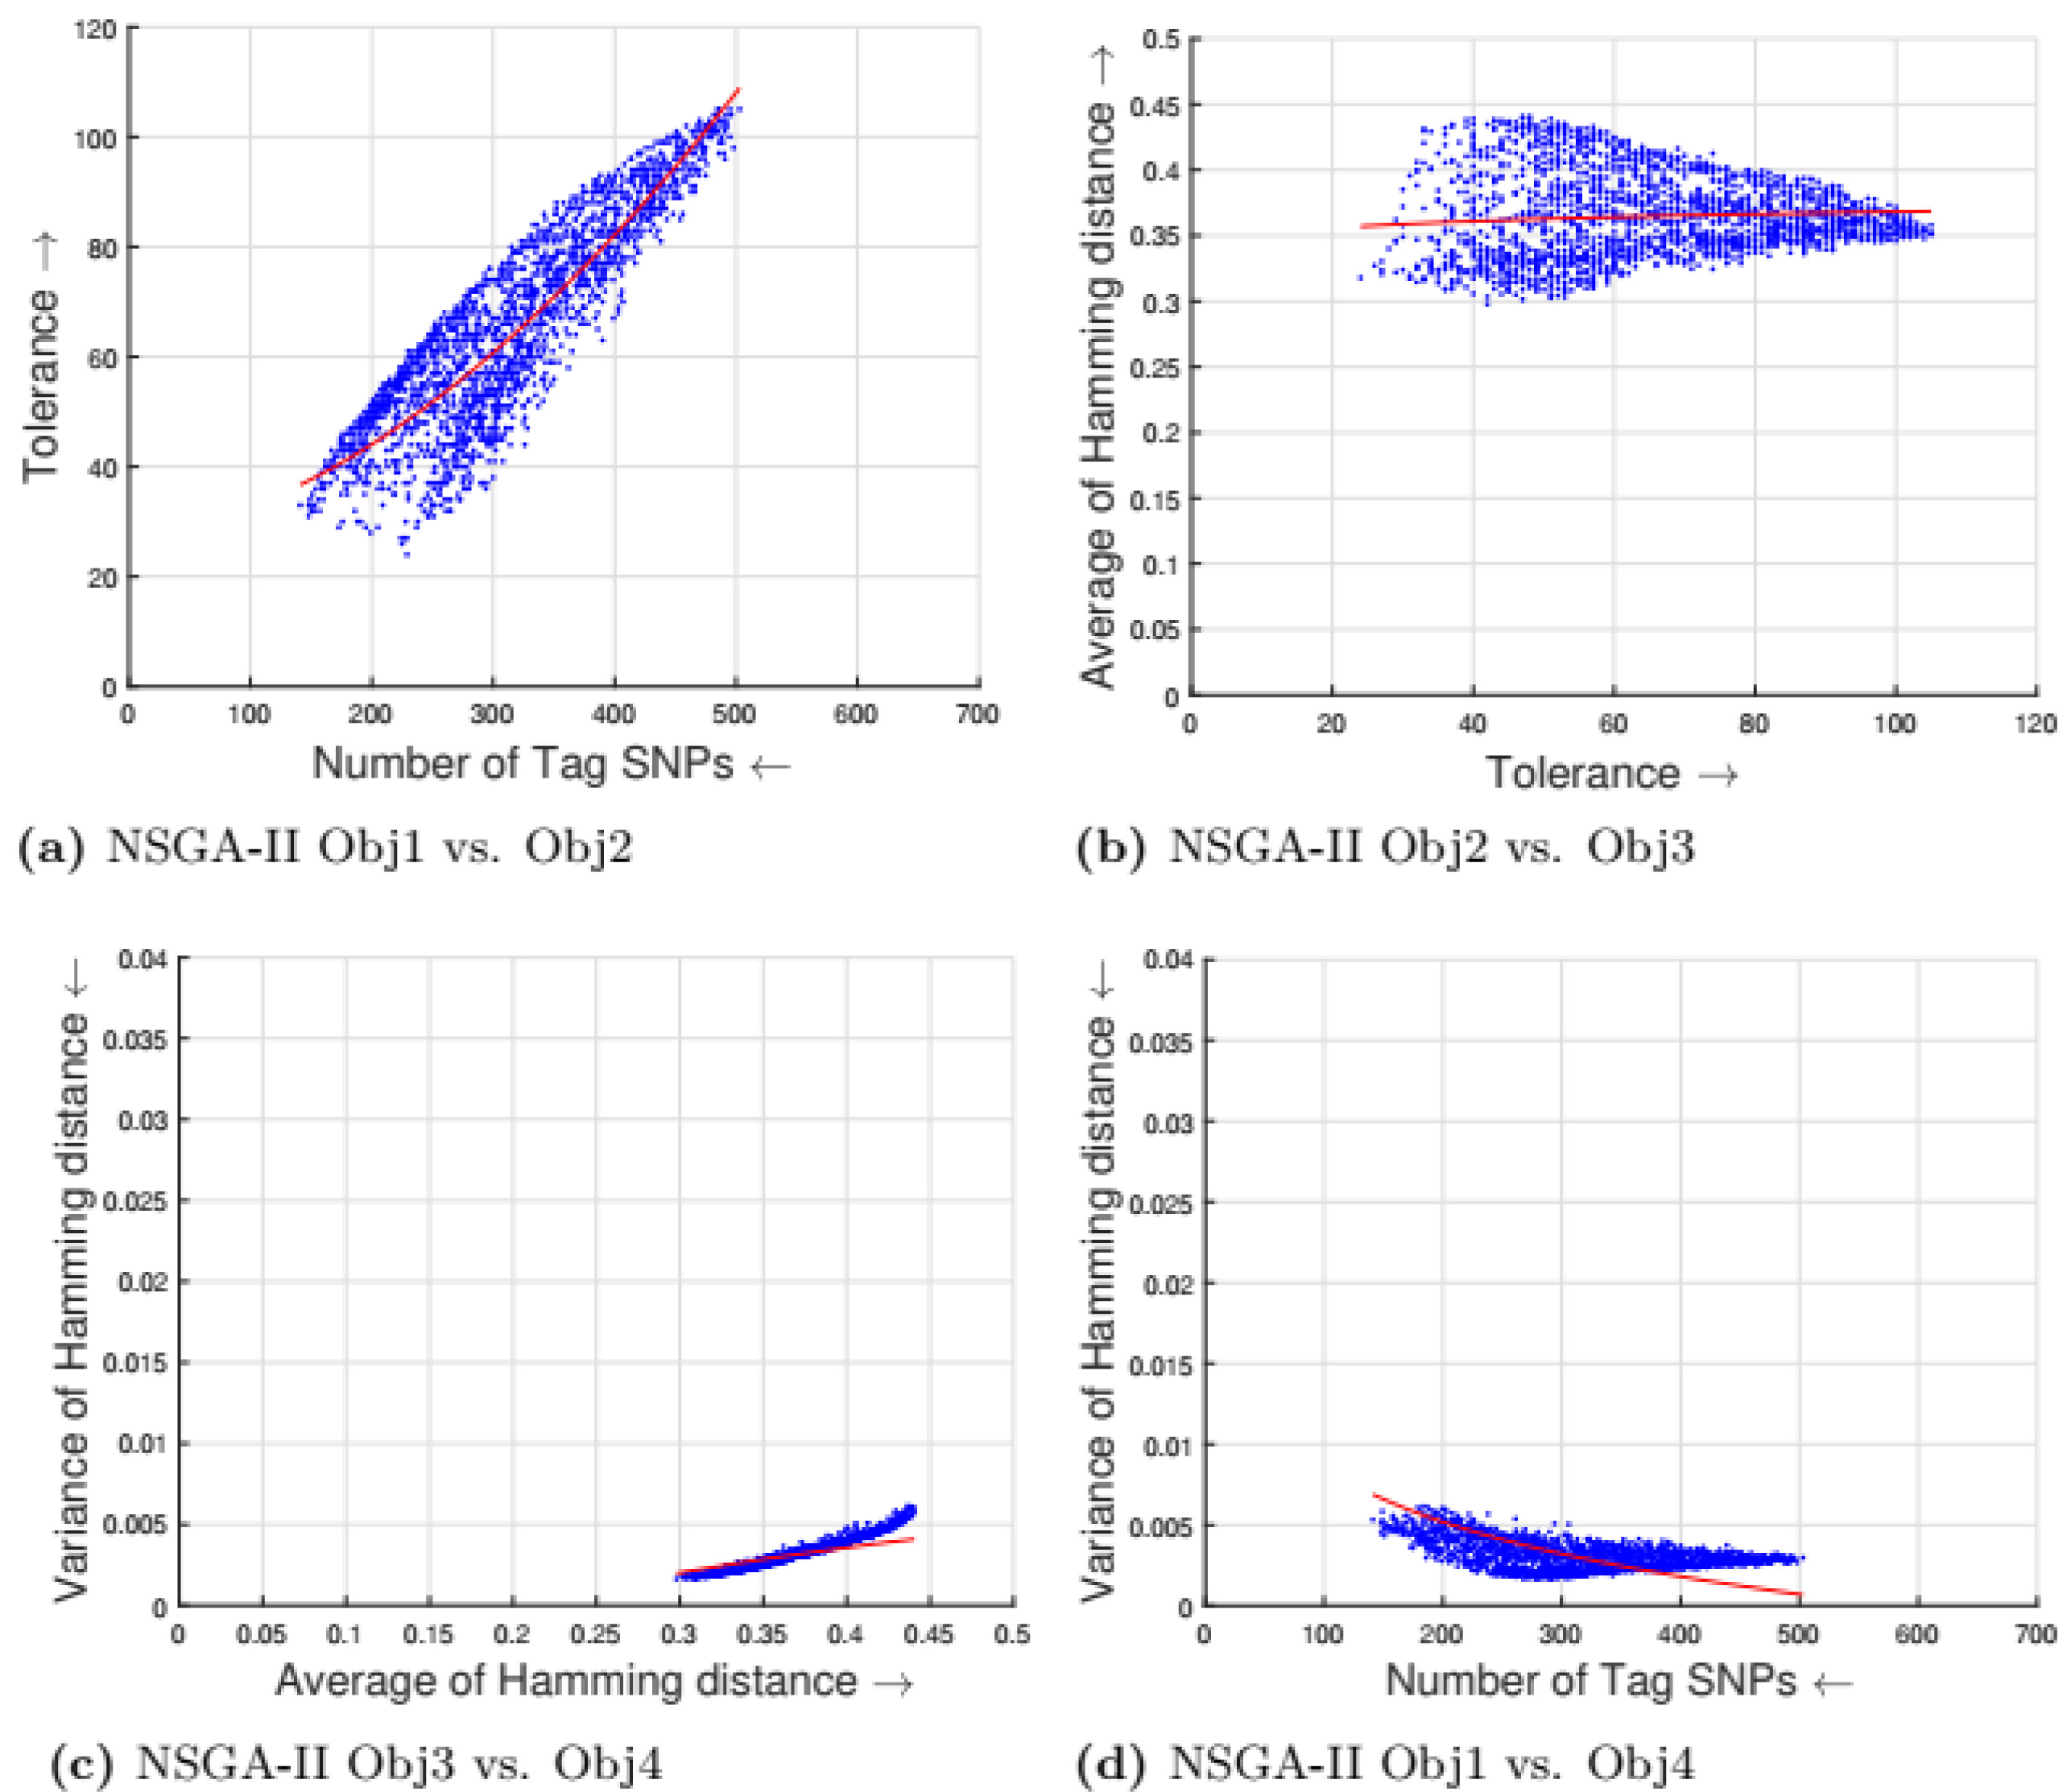
\includegraphics[width=0.18\textwidth]{analisis_assets/moqa_2022/figures/moqa_fig_nsga2_greedy.jpeg} &
        
\includegraphics[width=0.18\textwidth]{analisis_assets/20260430T185224/2_comparativa/1_frentes/frentes_pareto/frentes_pareto_nsga2_greedy_ting_full.png} &
        
\includegraphics[width=0.18\textwidth]{analisis_assets/20260430T185224/2_comparativa/1_frentes/frentes_pareto/frentes_pareto_nsga2_greedy_hybrid_full.png} &
        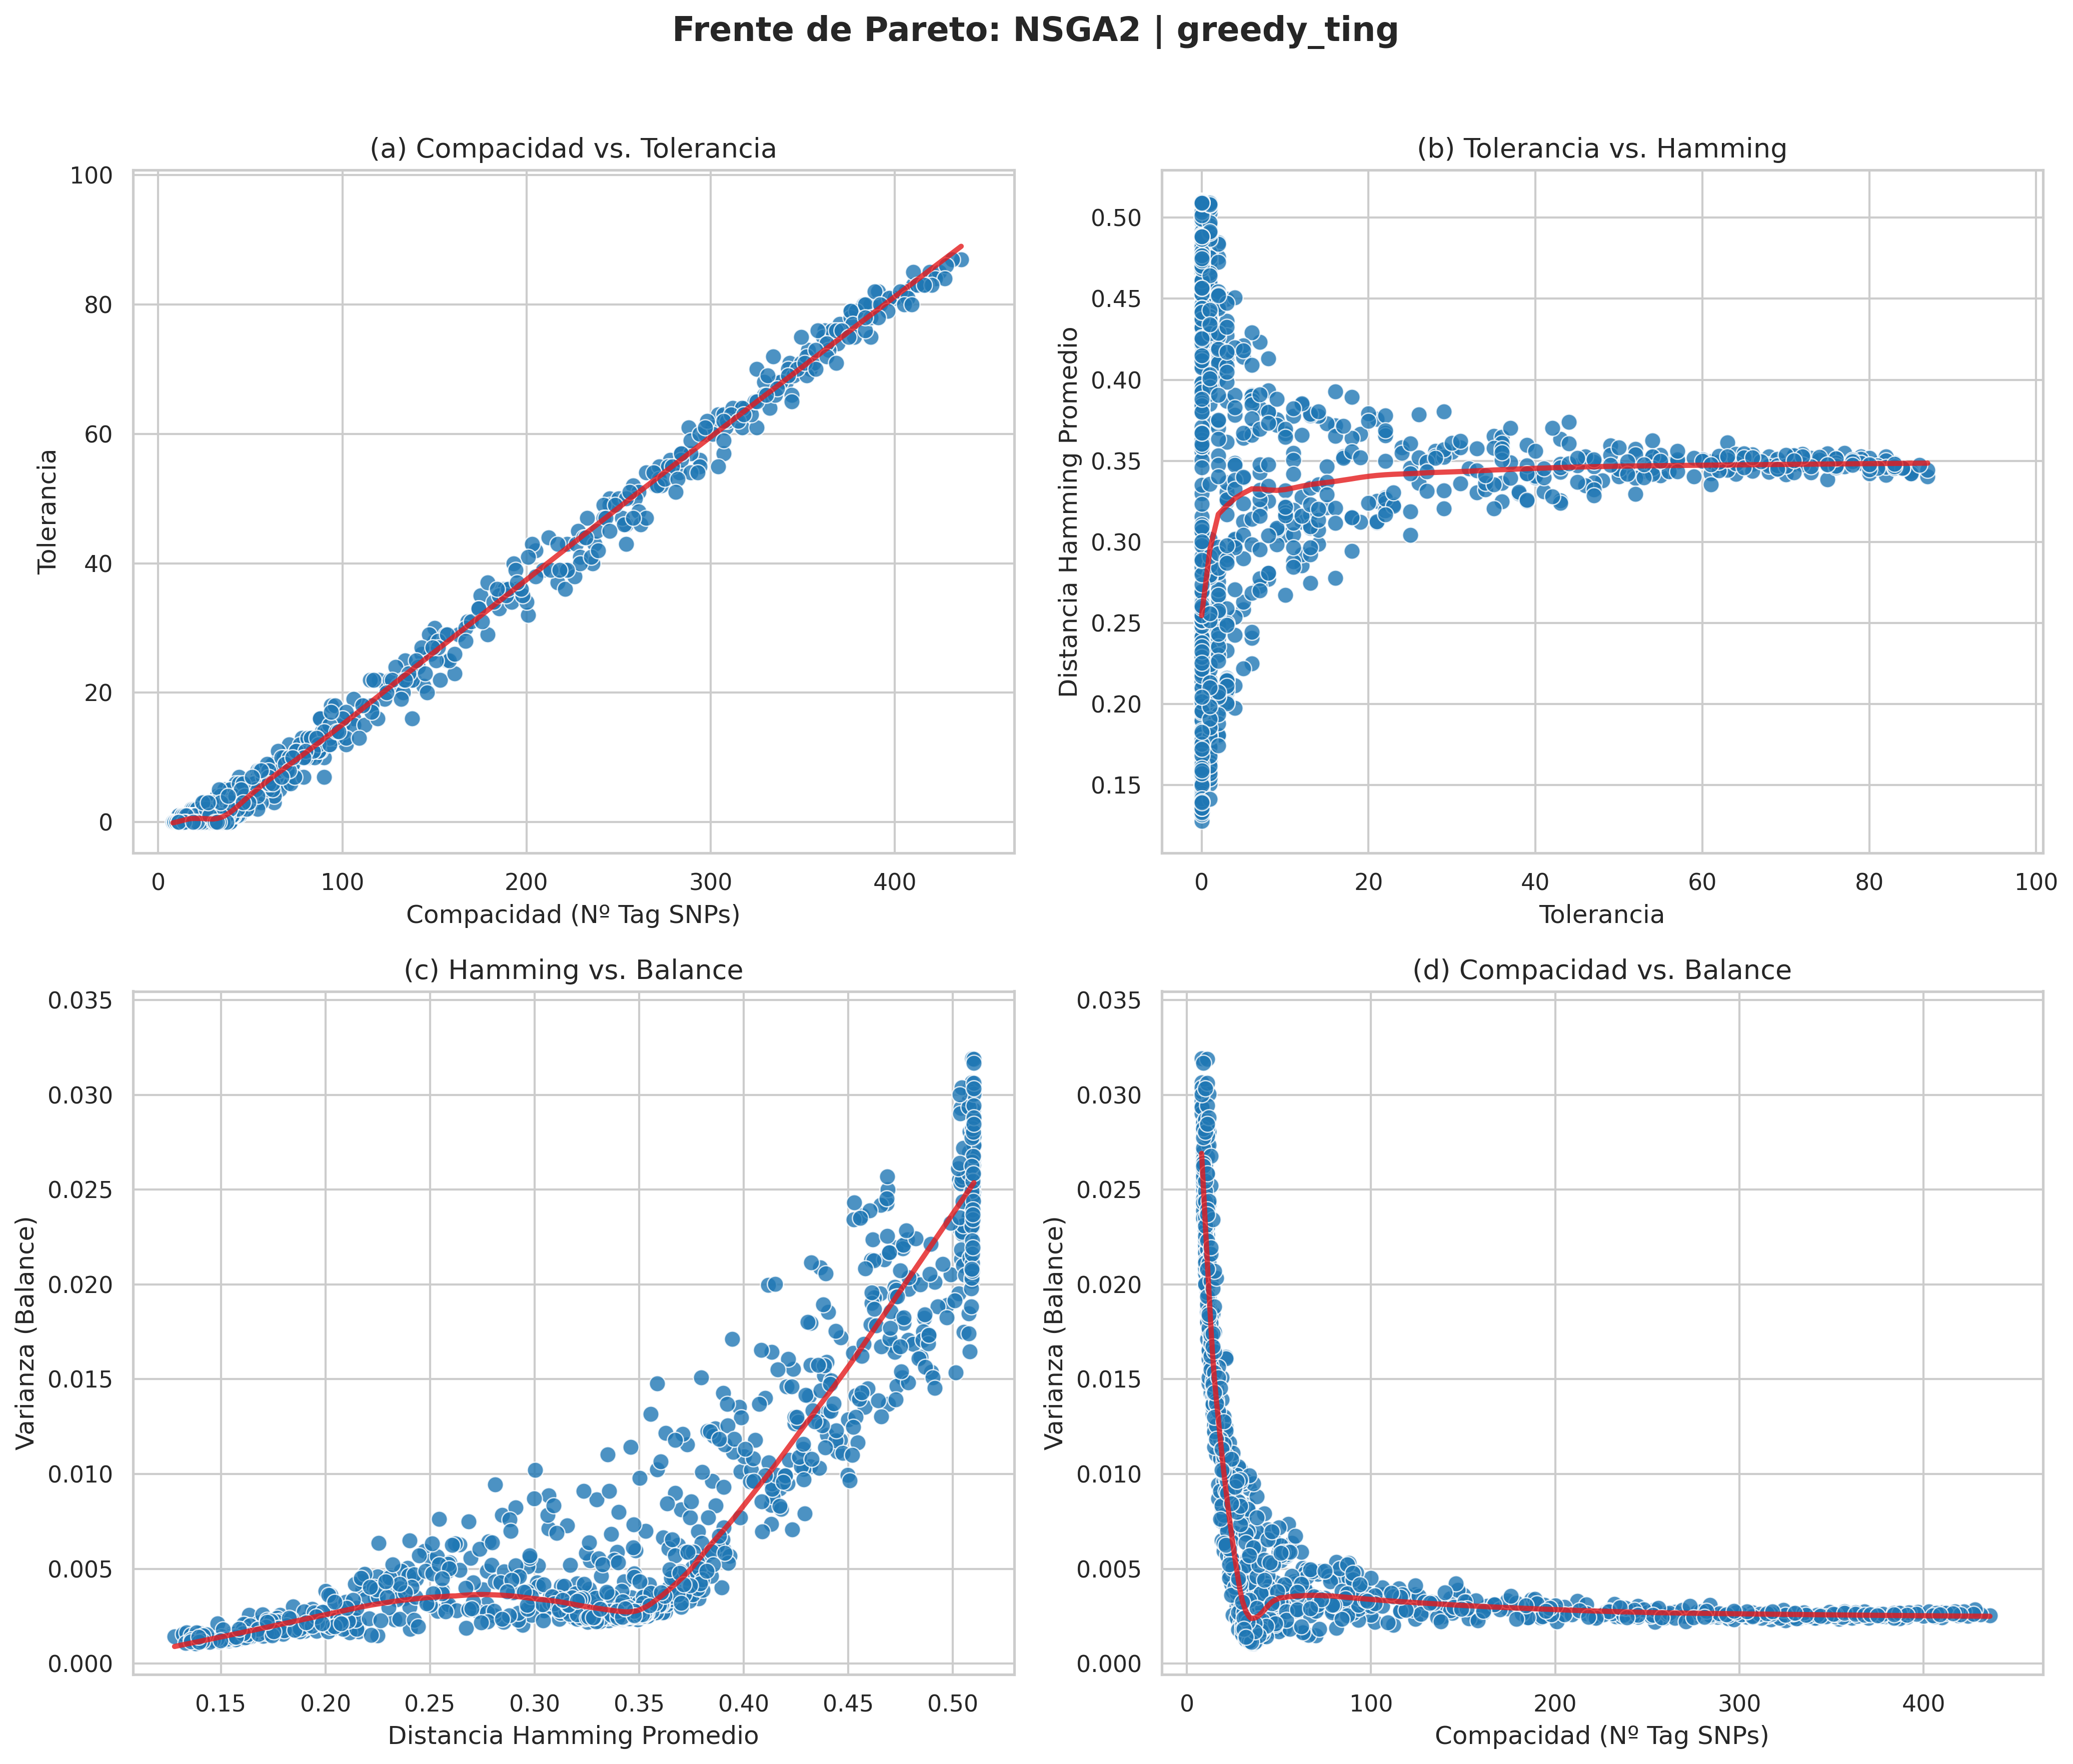
\includegraphics[width=0.18\textwidth]{analisis_assets/20260430T183144/2_comparativa/1_frentes/frentes_pareto/frentes_pareto_nsga2_greedy_ting_full.png} &
        
\includegraphics[width=0.18\textwidth]{analisis_assets/20260430T183144/2_comparativa/1_frentes/frentes_pareto/frentes_pareto_nsga2_greedy_hybrid_full.png} \\
        Moqa & Exp. A (GT) & Exp. A (GH) & Exp. B (GT) & Exp. B (GH) \\
    \end{tabular}
    \caption{Comparativa de frentes Greedy para NSGA-II frente al original de Moqa.}
\end{figure}

\begin{itemize}
    \item \textbf{Similitudes:} Las ejecuciones A y B presentan frentes con una morfología y distribución de puntos muy parecida. 
    \item \textbf{Diferencias:} Se observa una diferencia notable respecto a los frentes de Moqa, especialmente en la densidad de las soluciones encontradas. 
\end{itemize}

\begin{figure}[H]
    \centering
    \begin{tabular}{@{}ccc@{}}
        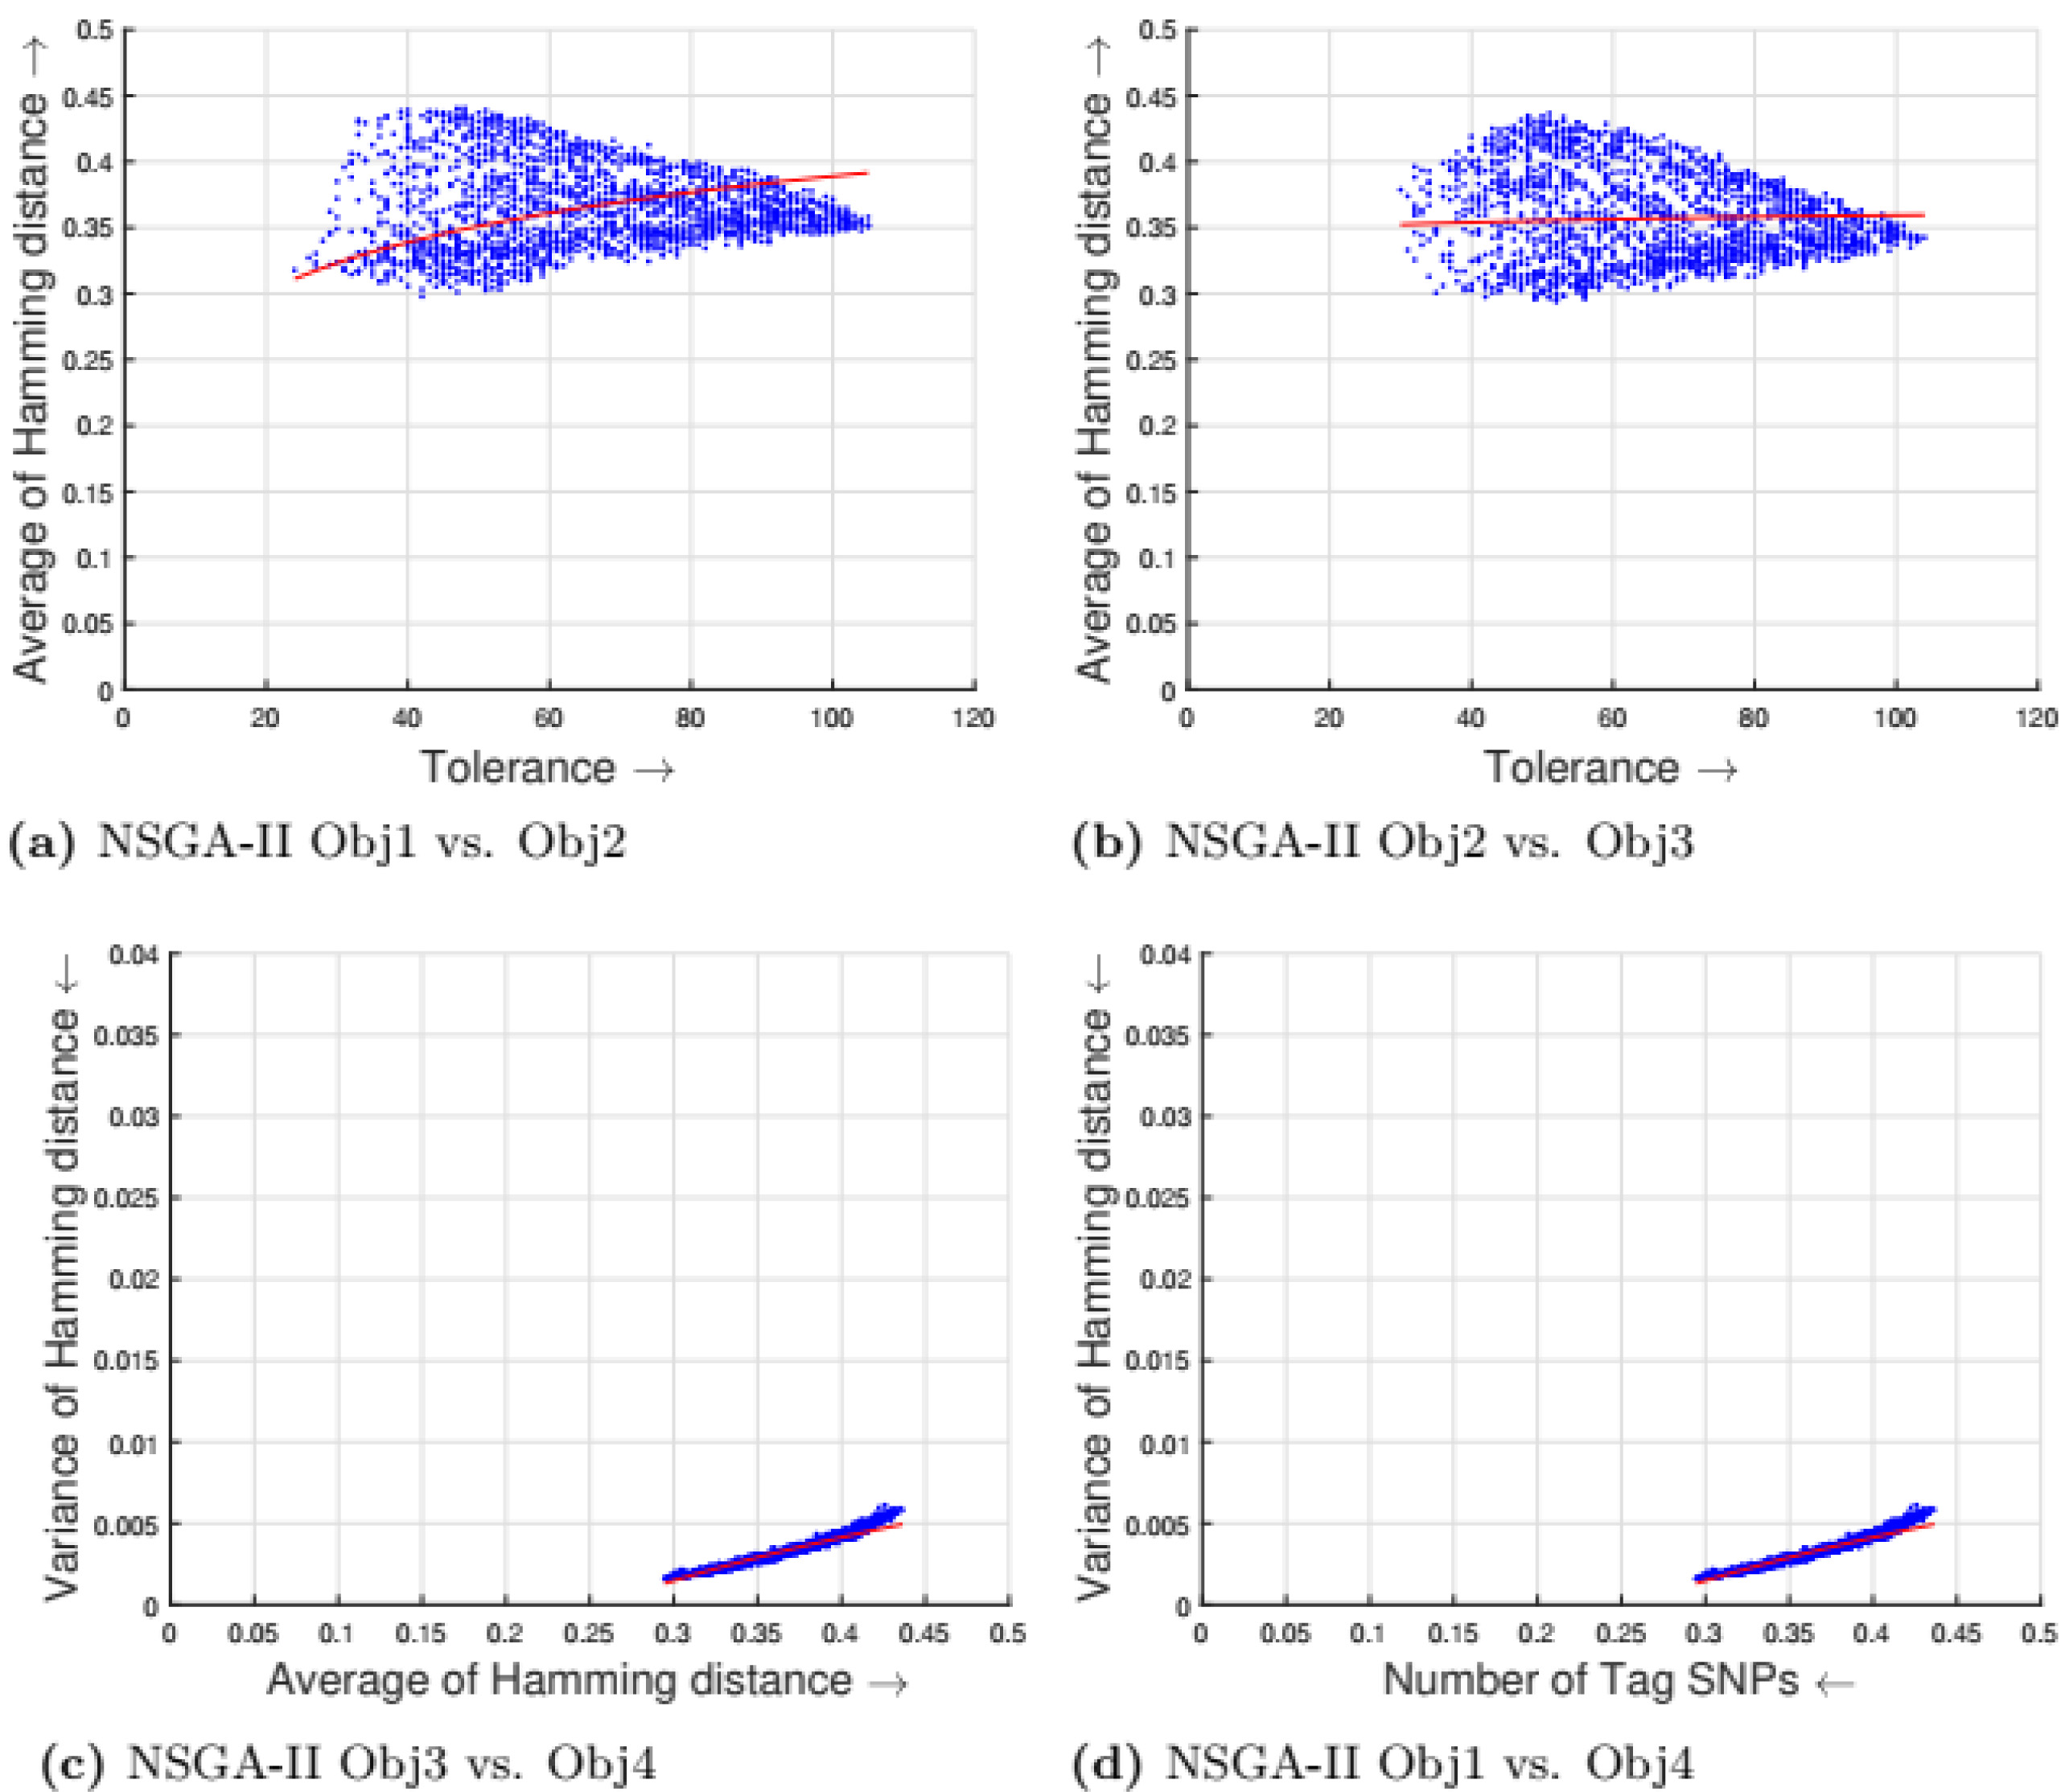
\includegraphics[width=0.28\textwidth]{analisis_assets/moqa_2022/figures/moqa_fig_nsga2_random.jpeg} &
        
\includegraphics[width=0.28\textwidth]{analisis_assets/20260430T185224/2_comparativa/1_frentes/frentes_pareto/frentes_pareto_nsga2_random_dense_full.png} &
        
\includegraphics[width=0.28\textwidth]{analisis_assets/20260430T183144/2_comparativa/1_frentes/frentes_pareto/frentes_pareto_nsga2_random_dense_full.png} \\
        Moqa & Exp. A (RD) & Exp. B (RD) \\
    \end{tabular}
    \caption{Comparativa de frentes Random para NSGA-II frente al original de Moqa.}
\end{figure}

\begin{itemize}
    \item \textbf{Similitudes:} En términos de posicionamiento en el espacio de objetivos, los frentes de A y B son muy similares a los de Moqa, a excepción de la proyección (0,1).
    \item \textbf{Diferencias:} El conjunto (0,1) de Moqa se desvía de lo observado en A y B. En general, los frentes obtenidos muestran una mayor extensión y cobertura del espacio.
\end{itemize}

\subsubsection{Comparativa Algoritmo SPEA2}

\begin{figure}[H]
    \centering
    \begin{tabular}{@{}ccccc@{}}
        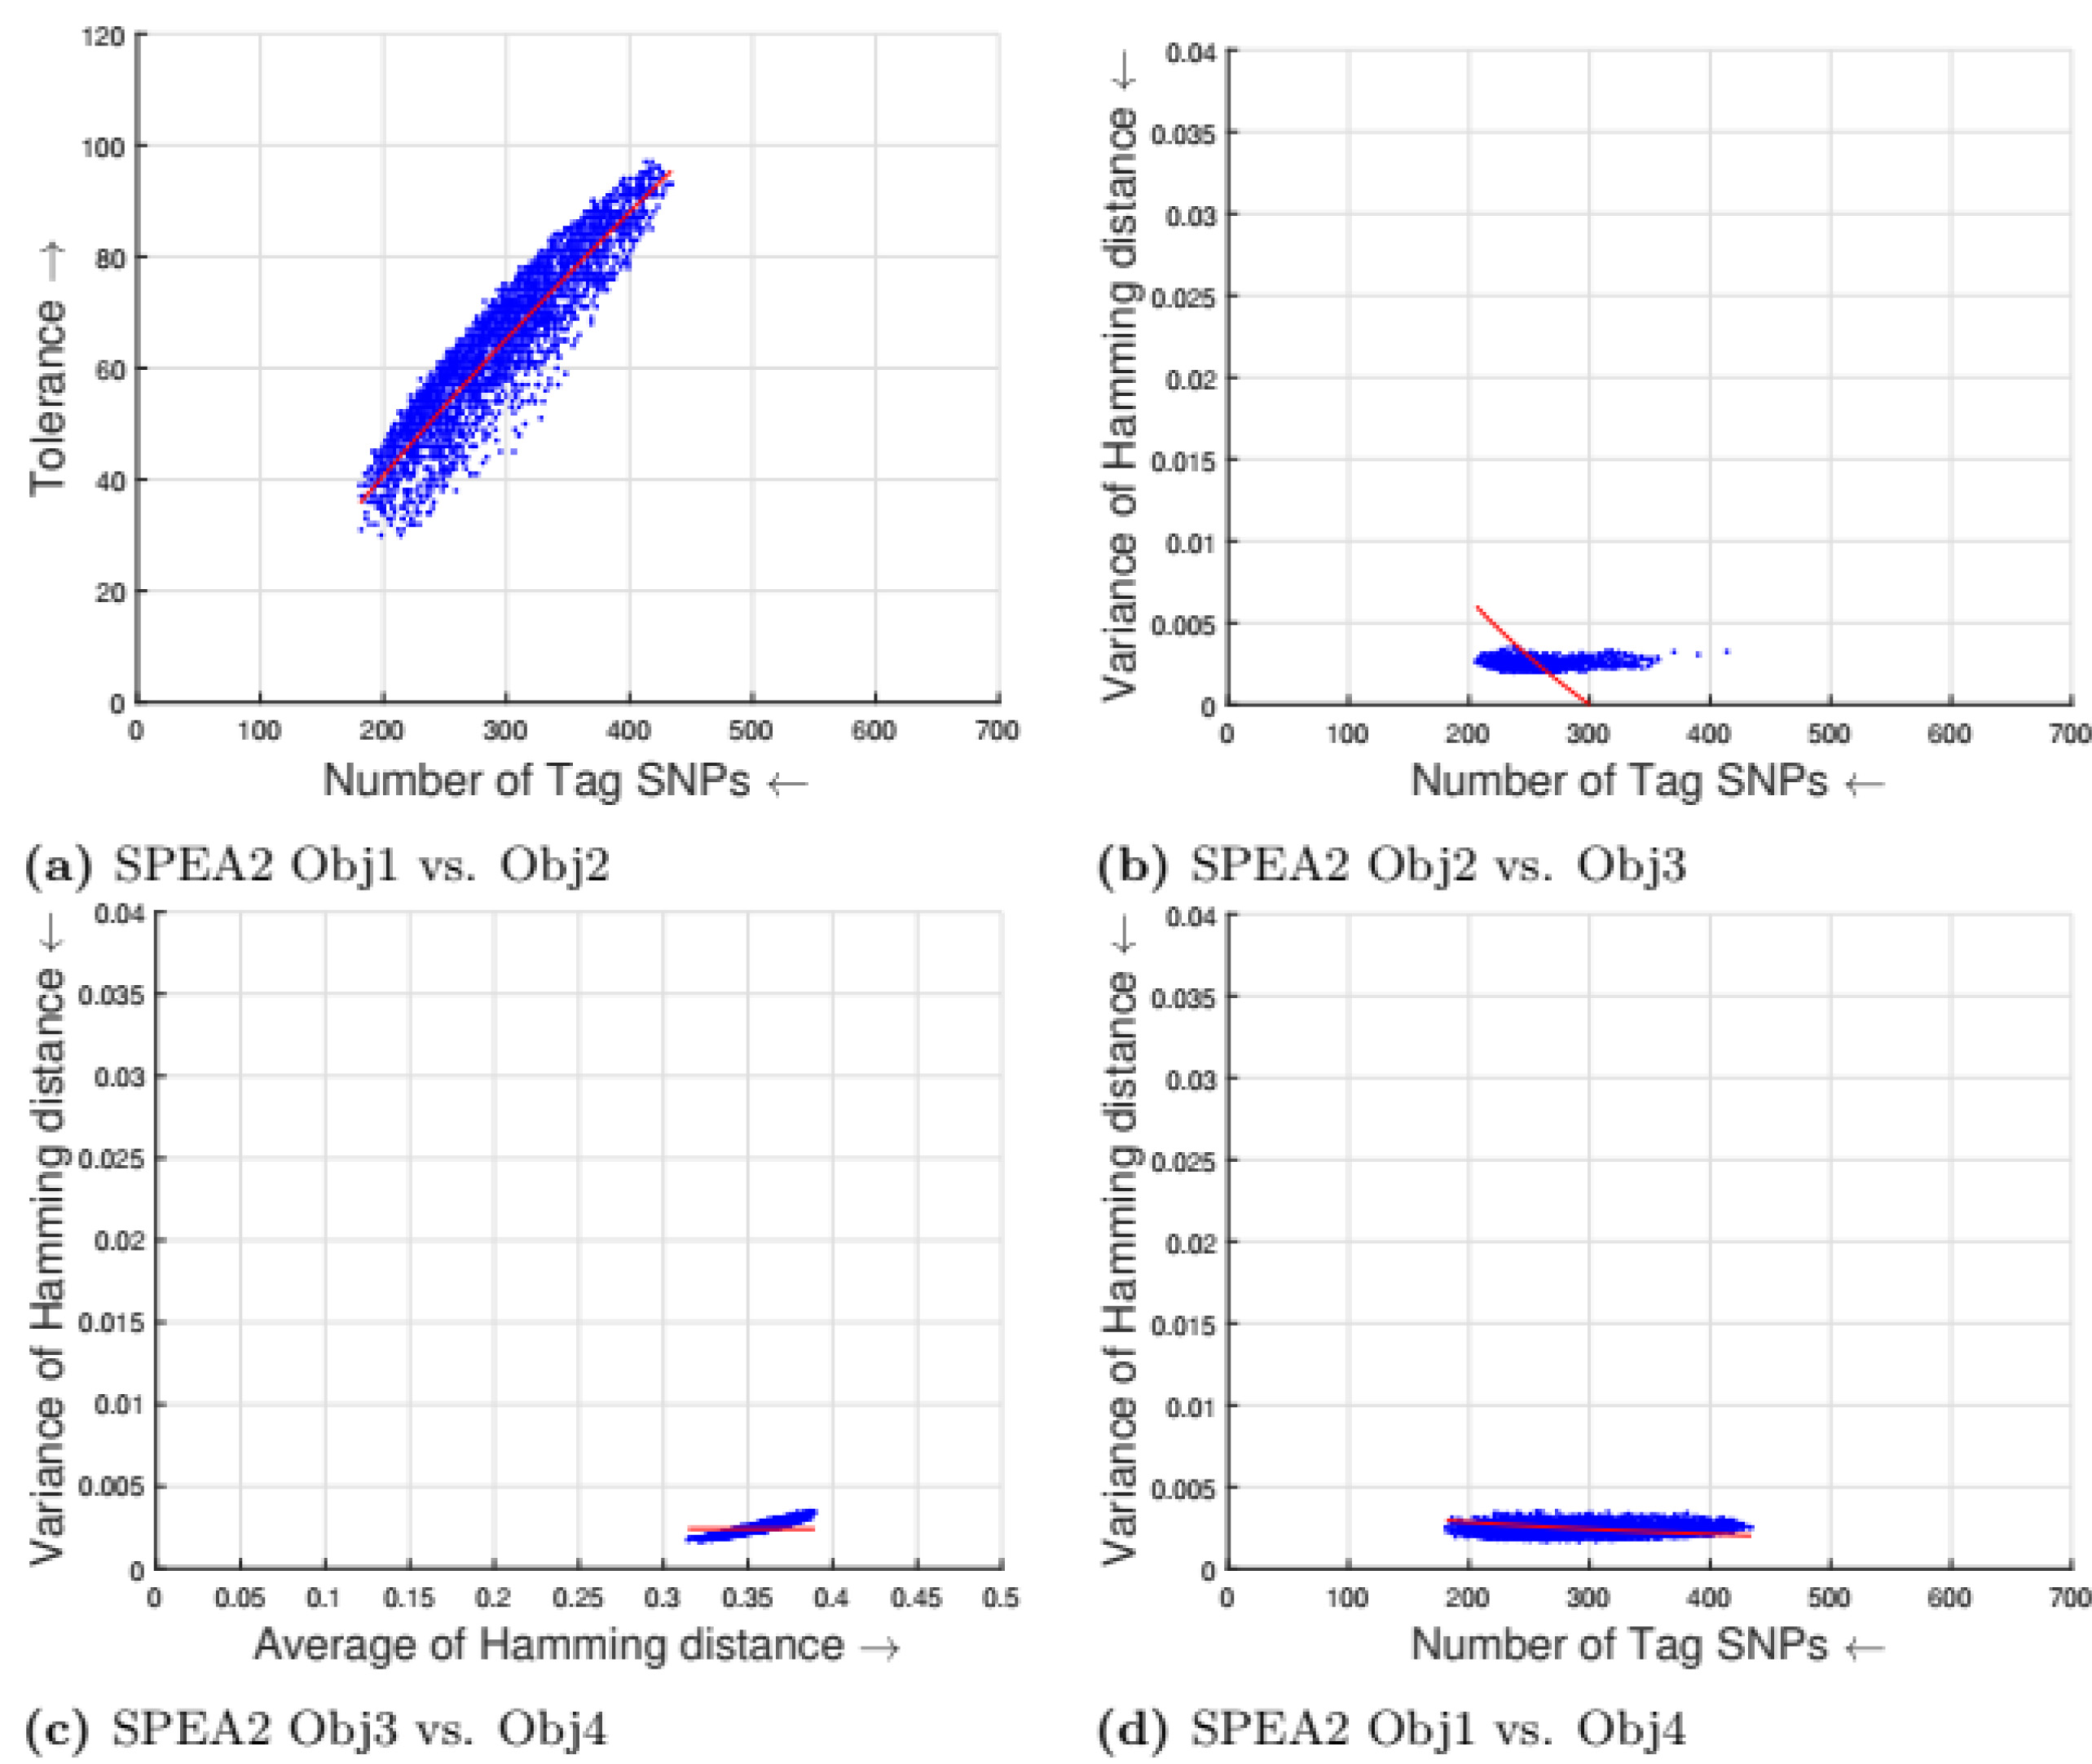
\includegraphics[width=0.18\textwidth]{analisis_assets/moqa_2022/figures/moqa_fig_spea2_greedy.jpeg} &
        
\includegraphics[width=0.18\textwidth]{analisis_assets/20260430T185224/2_comparativa/1_frentes/frentes_pareto/frentes_pareto_spea2_greedy_ting_full.png} &
        
\includegraphics[width=0.18\textwidth]{analisis_assets/20260430T185224/2_comparativa/1_frentes/frentes_pareto/frentes_pareto_spea2_greedy_hybrid_full.png} &
        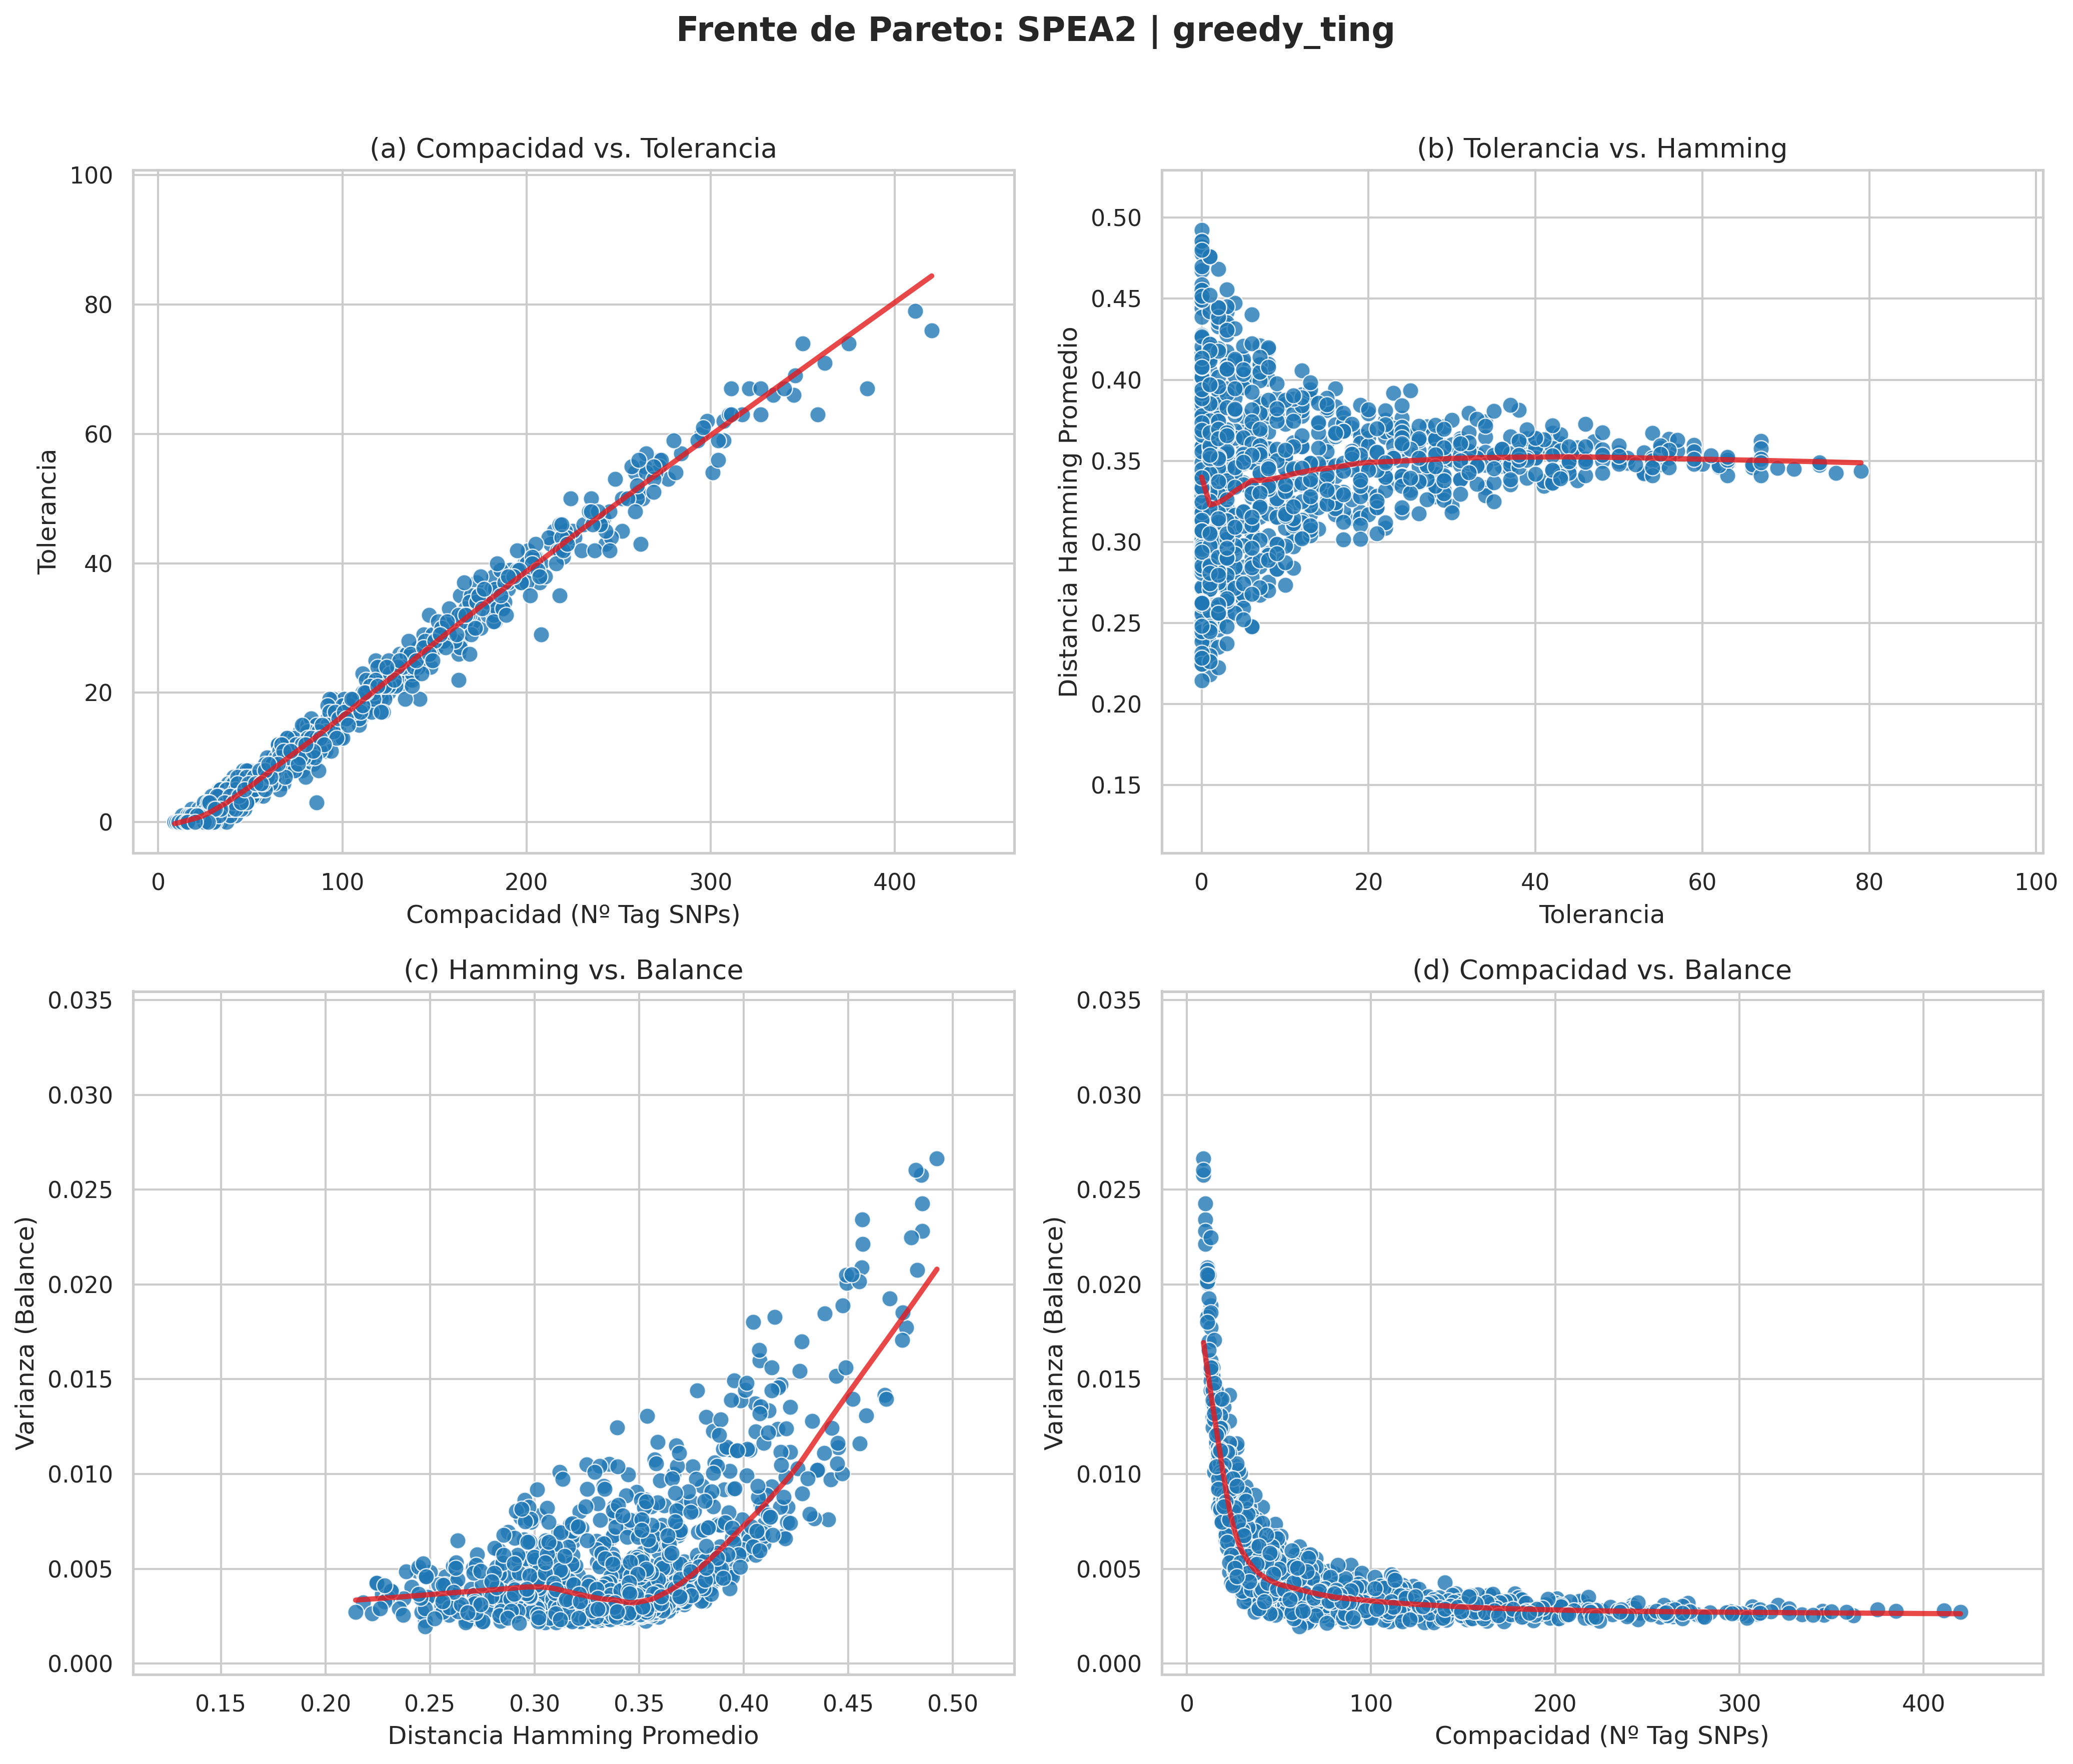
\includegraphics[width=0.18\textwidth]{analisis_assets/20260430T183144/2_comparativa/1_frentes/frentes_pareto/frentes_pareto_spea2_greedy_ting_full.png} &
        
\includegraphics[width=0.18\textwidth]{analisis_assets/20260430T183144/2_comparativa/1_frentes/frentes_pareto/frentes_pareto_spea2_greedy_hybrid_full.png} \\
        Moqa & Exp. A (GT) & Exp. A (GH) & Exp. B (GT) & Exp. B (GH) \\
    \end{tabular}
    \caption{Comparativa de frentes Greedy para SPEA2 frente al original de Moqa.}
\end{figure}

\begin{itemize}
    \item \textbf{Similitudes:} Existe una concordancia razonable en la topología del frente para la proyección (0,1).
    \item \textbf{Diferencias:} Los frentes de A y B consiguen una mayor amplitud que los de Moqa. Al margen del frente (0,1), las diferencias cualitativas con el estudio original son bastante marcadas.
\end{itemize}

\begin{figure}[H]
    \centering
    \begin{tabular}{@{}ccc@{}}
        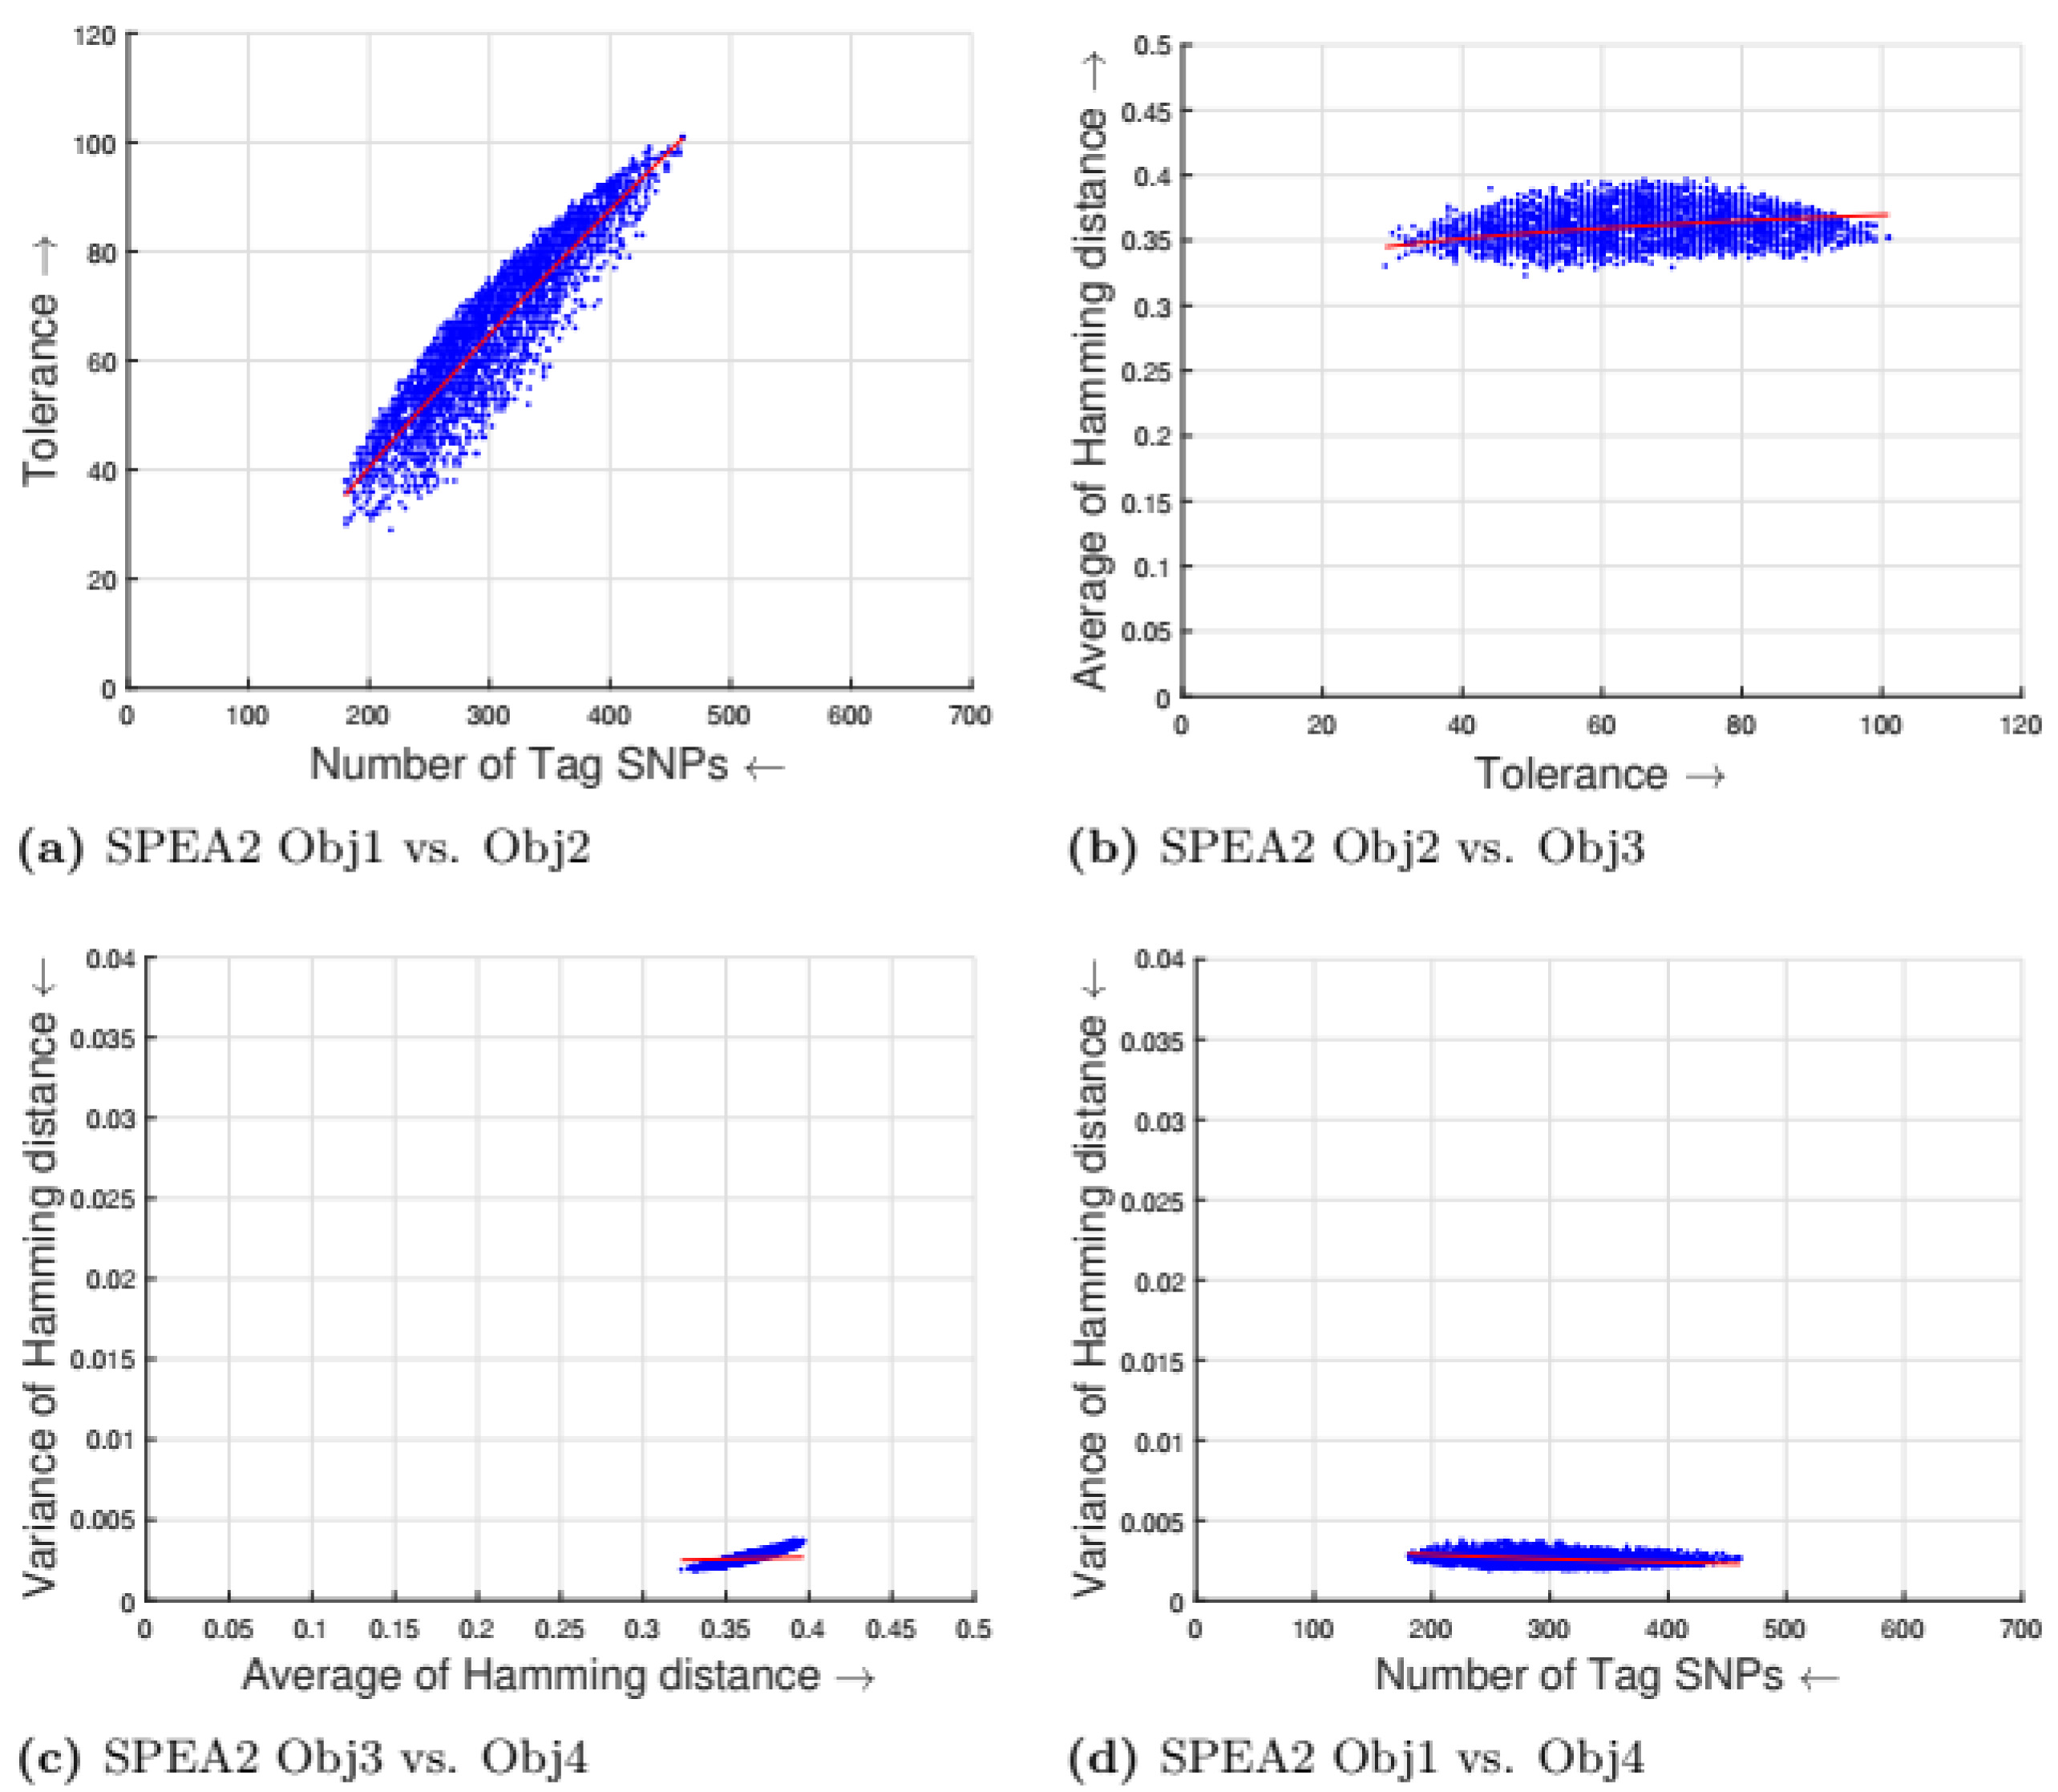
\includegraphics[width=0.28\textwidth]{analisis_assets/moqa_2022/figures/moqa_fig_spea2_random.jpeg} &
        
\includegraphics[width=0.28\textwidth]{analisis_assets/20260430T185224/2_comparativa/1_frentes/frentes_pareto/frentes_pareto_spea2_random_dense_full.png} &
        
\includegraphics[width=0.28\textwidth]{analisis_assets/20260430T183144/2_comparativa/1_frentes/frentes_pareto/frentes_pareto_spea2_random_dense_full.png} \\
        Moqa & Exp. A (RD) & Exp. B (RD) \\
    \end{tabular}
    \caption{Comparativa de frentes Random para SPEA2 frente al original de Moqa.}
\end{figure}

\begin{itemize}
    \item \textbf{Similitudes:} Se observa una gran similitud general entre los frentes, sin que se aprecien cambios estructurales de importancia.
    \item \textbf{Diferencias:} No se identifican diferencias cualitativas relevantes en esta comparativa.
\end{itemize}

\subsubsection{Comparativa Algoritmo NSGA-III}

\begin{figure}[H]
    \centering
    \begin{tabular}{@{}ccccc@{}}
        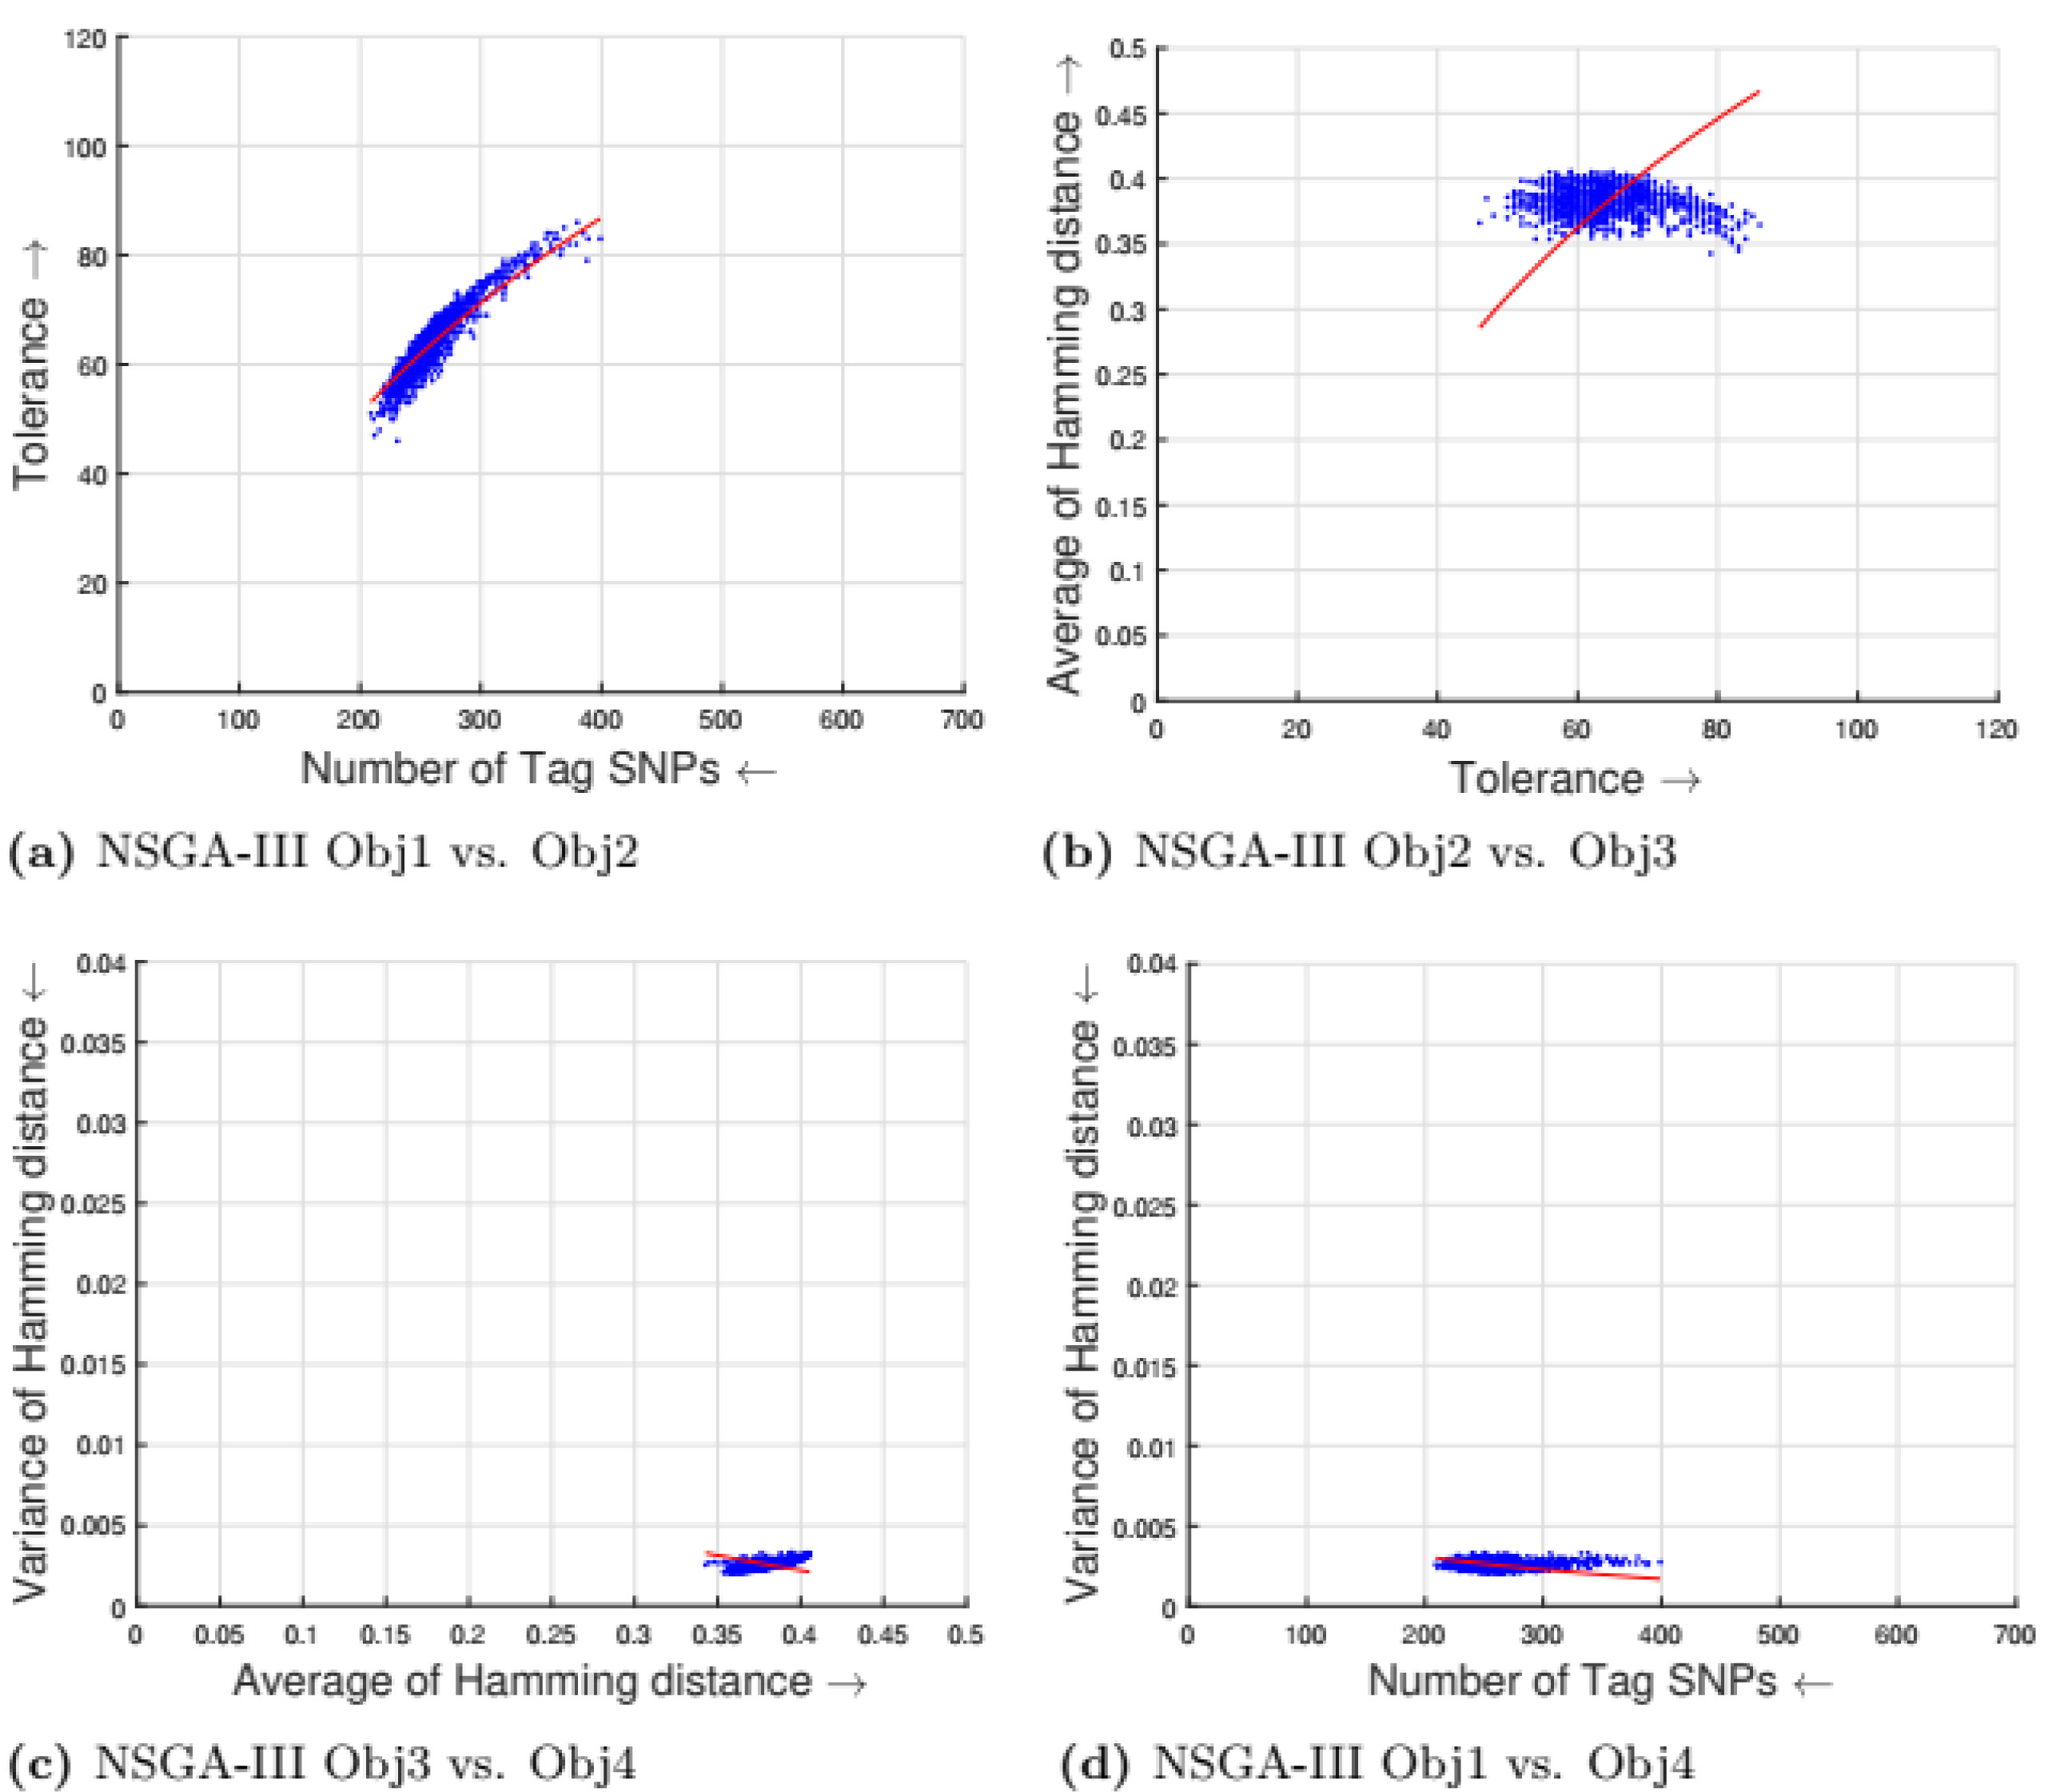
\includegraphics[width=0.18\textwidth]{analisis_assets/moqa_2022/figures/moqa_fig_nsga3_greedy.jpeg} &
        
\includegraphics[width=0.18\textwidth]{analisis_assets/20260430T185224/2_comparativa/1_frentes/frentes_pareto/frentes_pareto_nsga3_greedy_ting_full.png} &
        
\includegraphics[width=0.18\textwidth]{analisis_assets/20260430T185224/2_comparativa/1_frentes/frentes_pareto/frentes_pareto_nsga3_greedy_hybrid_full.png} &
        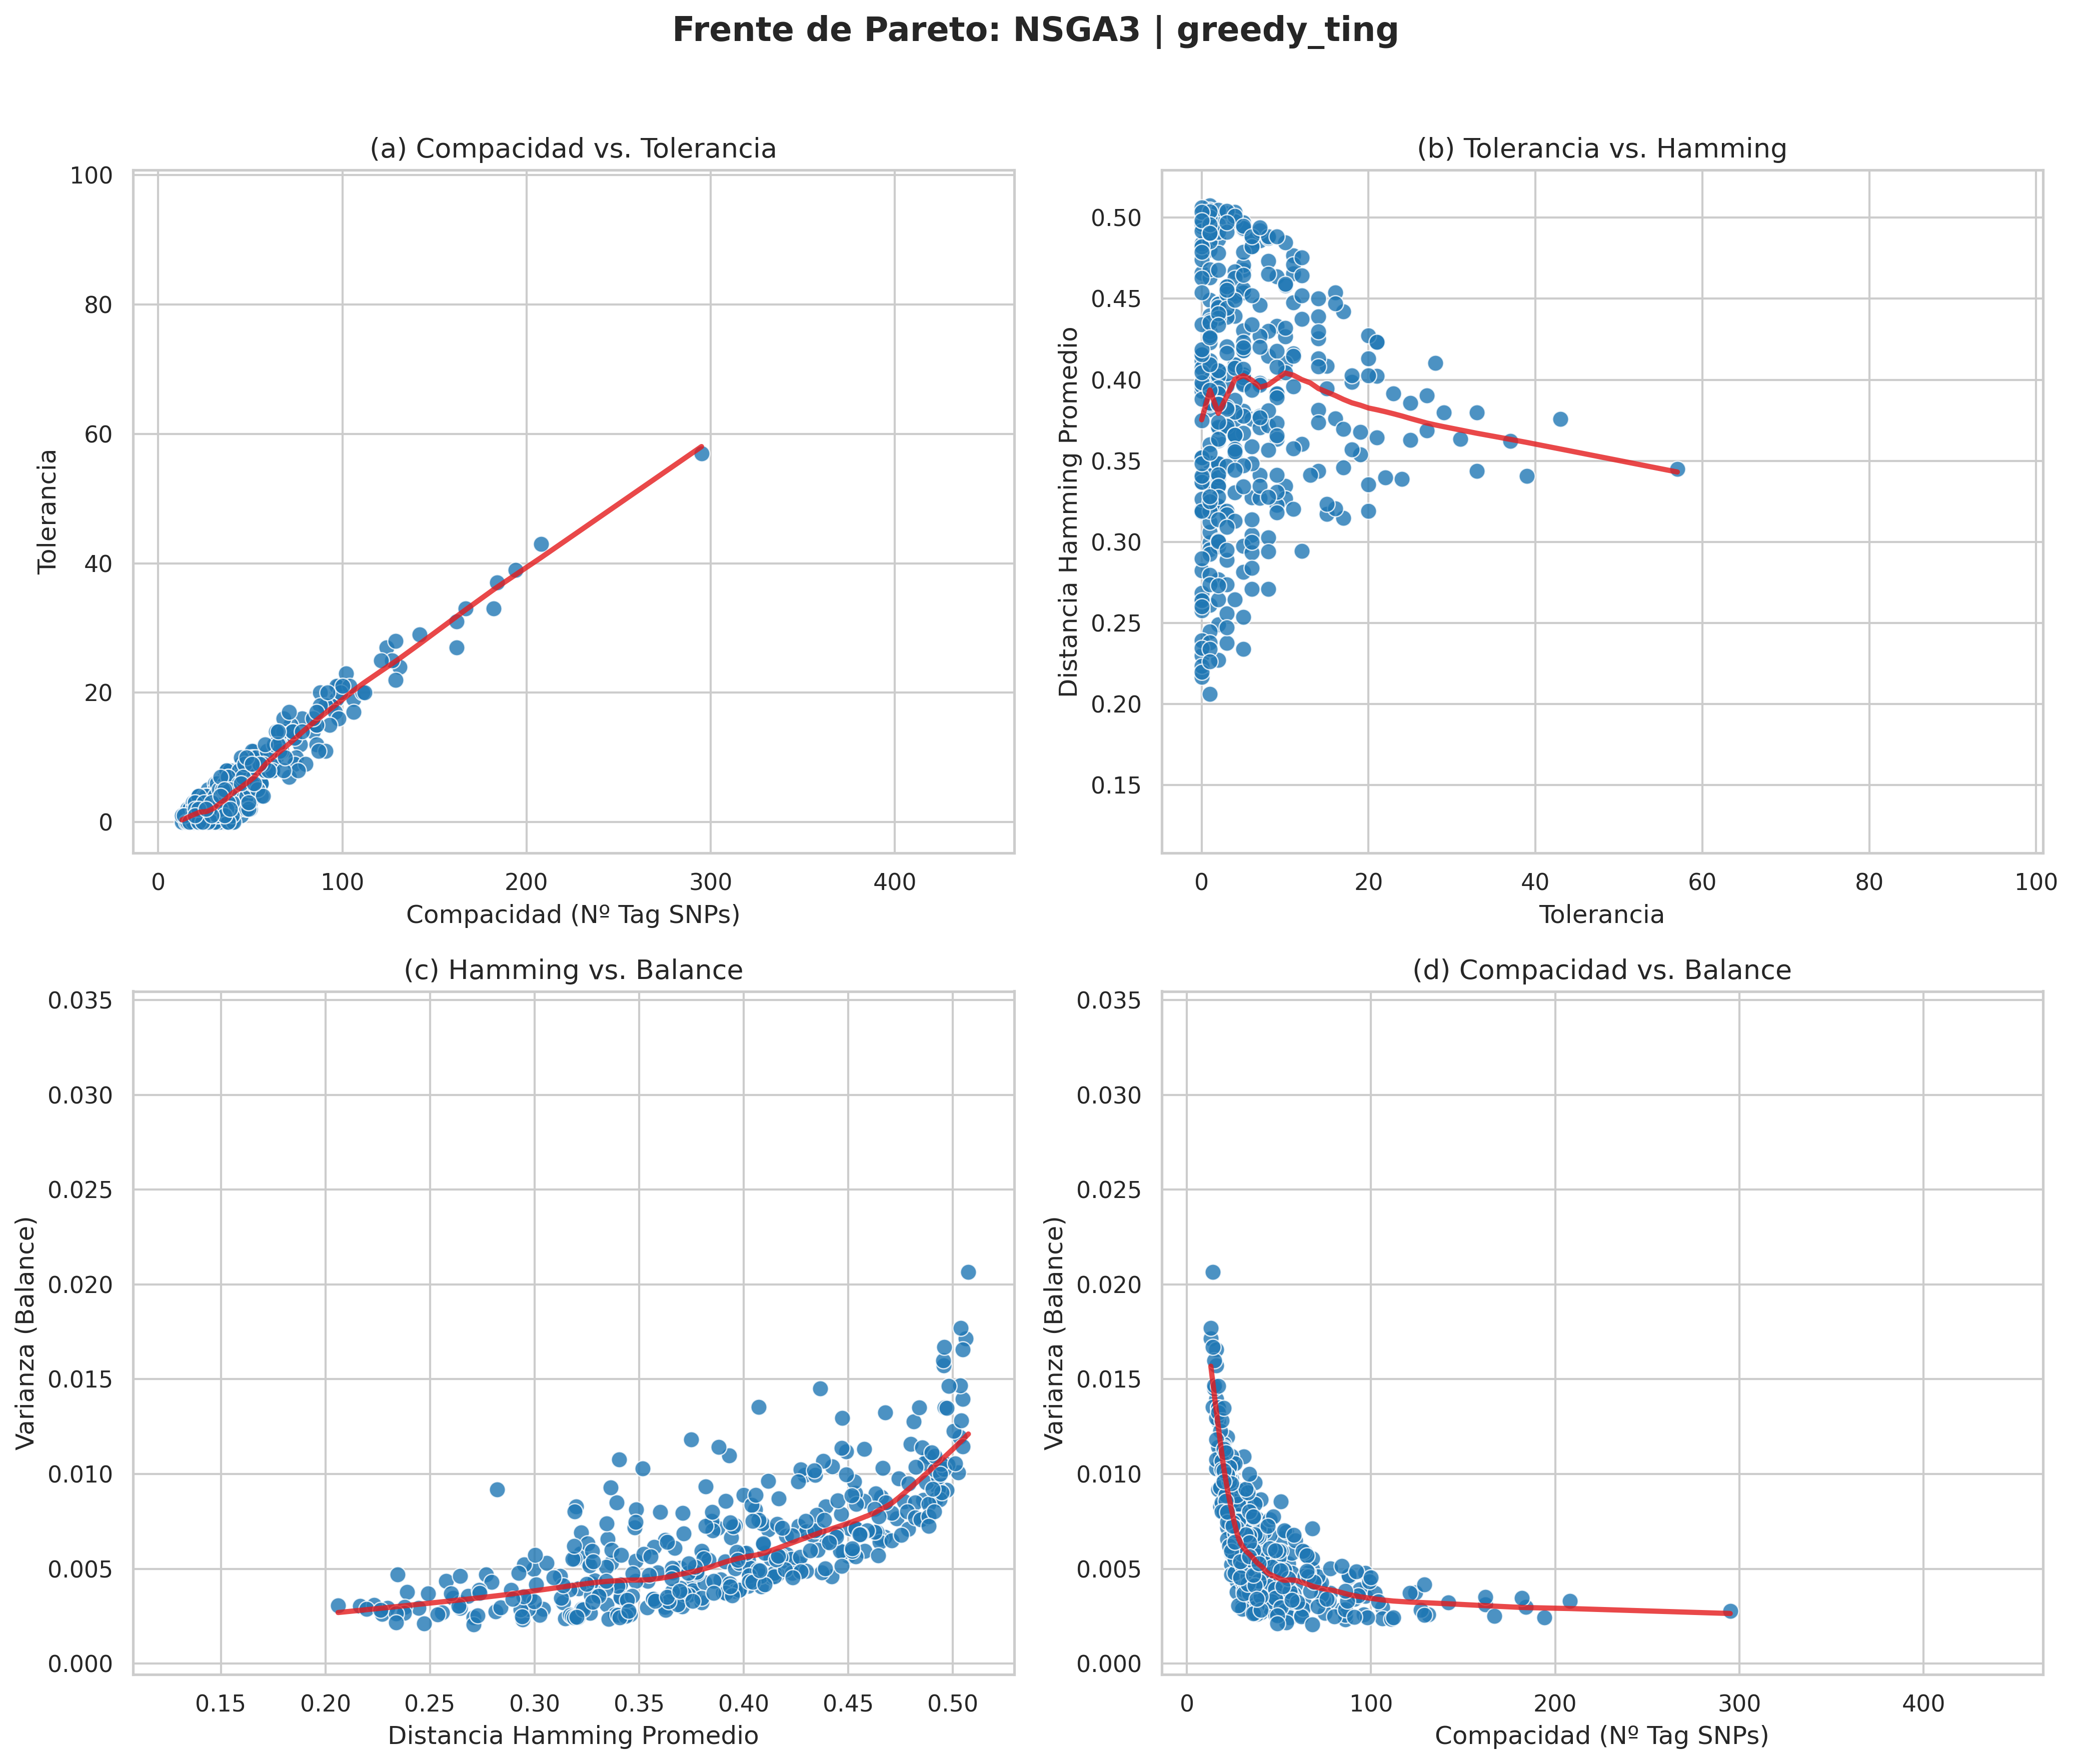
\includegraphics[width=0.18\textwidth]{analisis_assets/20260430T183144/2_comparativa/1_frentes/frentes_pareto/frentes_pareto_nsga3_greedy_ting_full.png} &
        
\includegraphics[width=0.18\textwidth]{analisis_assets/20260430T183144/2_comparativa/1_frentes/frentes_pareto/frentes_pareto_nsga3_greedy_hybrid_full.png} \\
        Moqa & Exp. A (GT) & Exp. A (GH) & Exp. B (GT) & Exp. B (GH) \\
    \end{tabular}
    \caption{Comparativa de frentes Greedy para NSGA-III frente al original de Moqa.}
\end{figure}

\begin{itemize}
    \item \textbf{Similitudes:} No se detectan muchas analogías claras entre los frentes comparados.
    \item \textbf{Diferencias:} Se repite la tendencia observada: los frentes de A y B resultan más extensos y cubren mejor el espacio de búsqueda que los de Moqa.
\end{itemize}

\begin{figure}[H]
    \centering
    \begin{tabular}{@{}ccc@{}}
        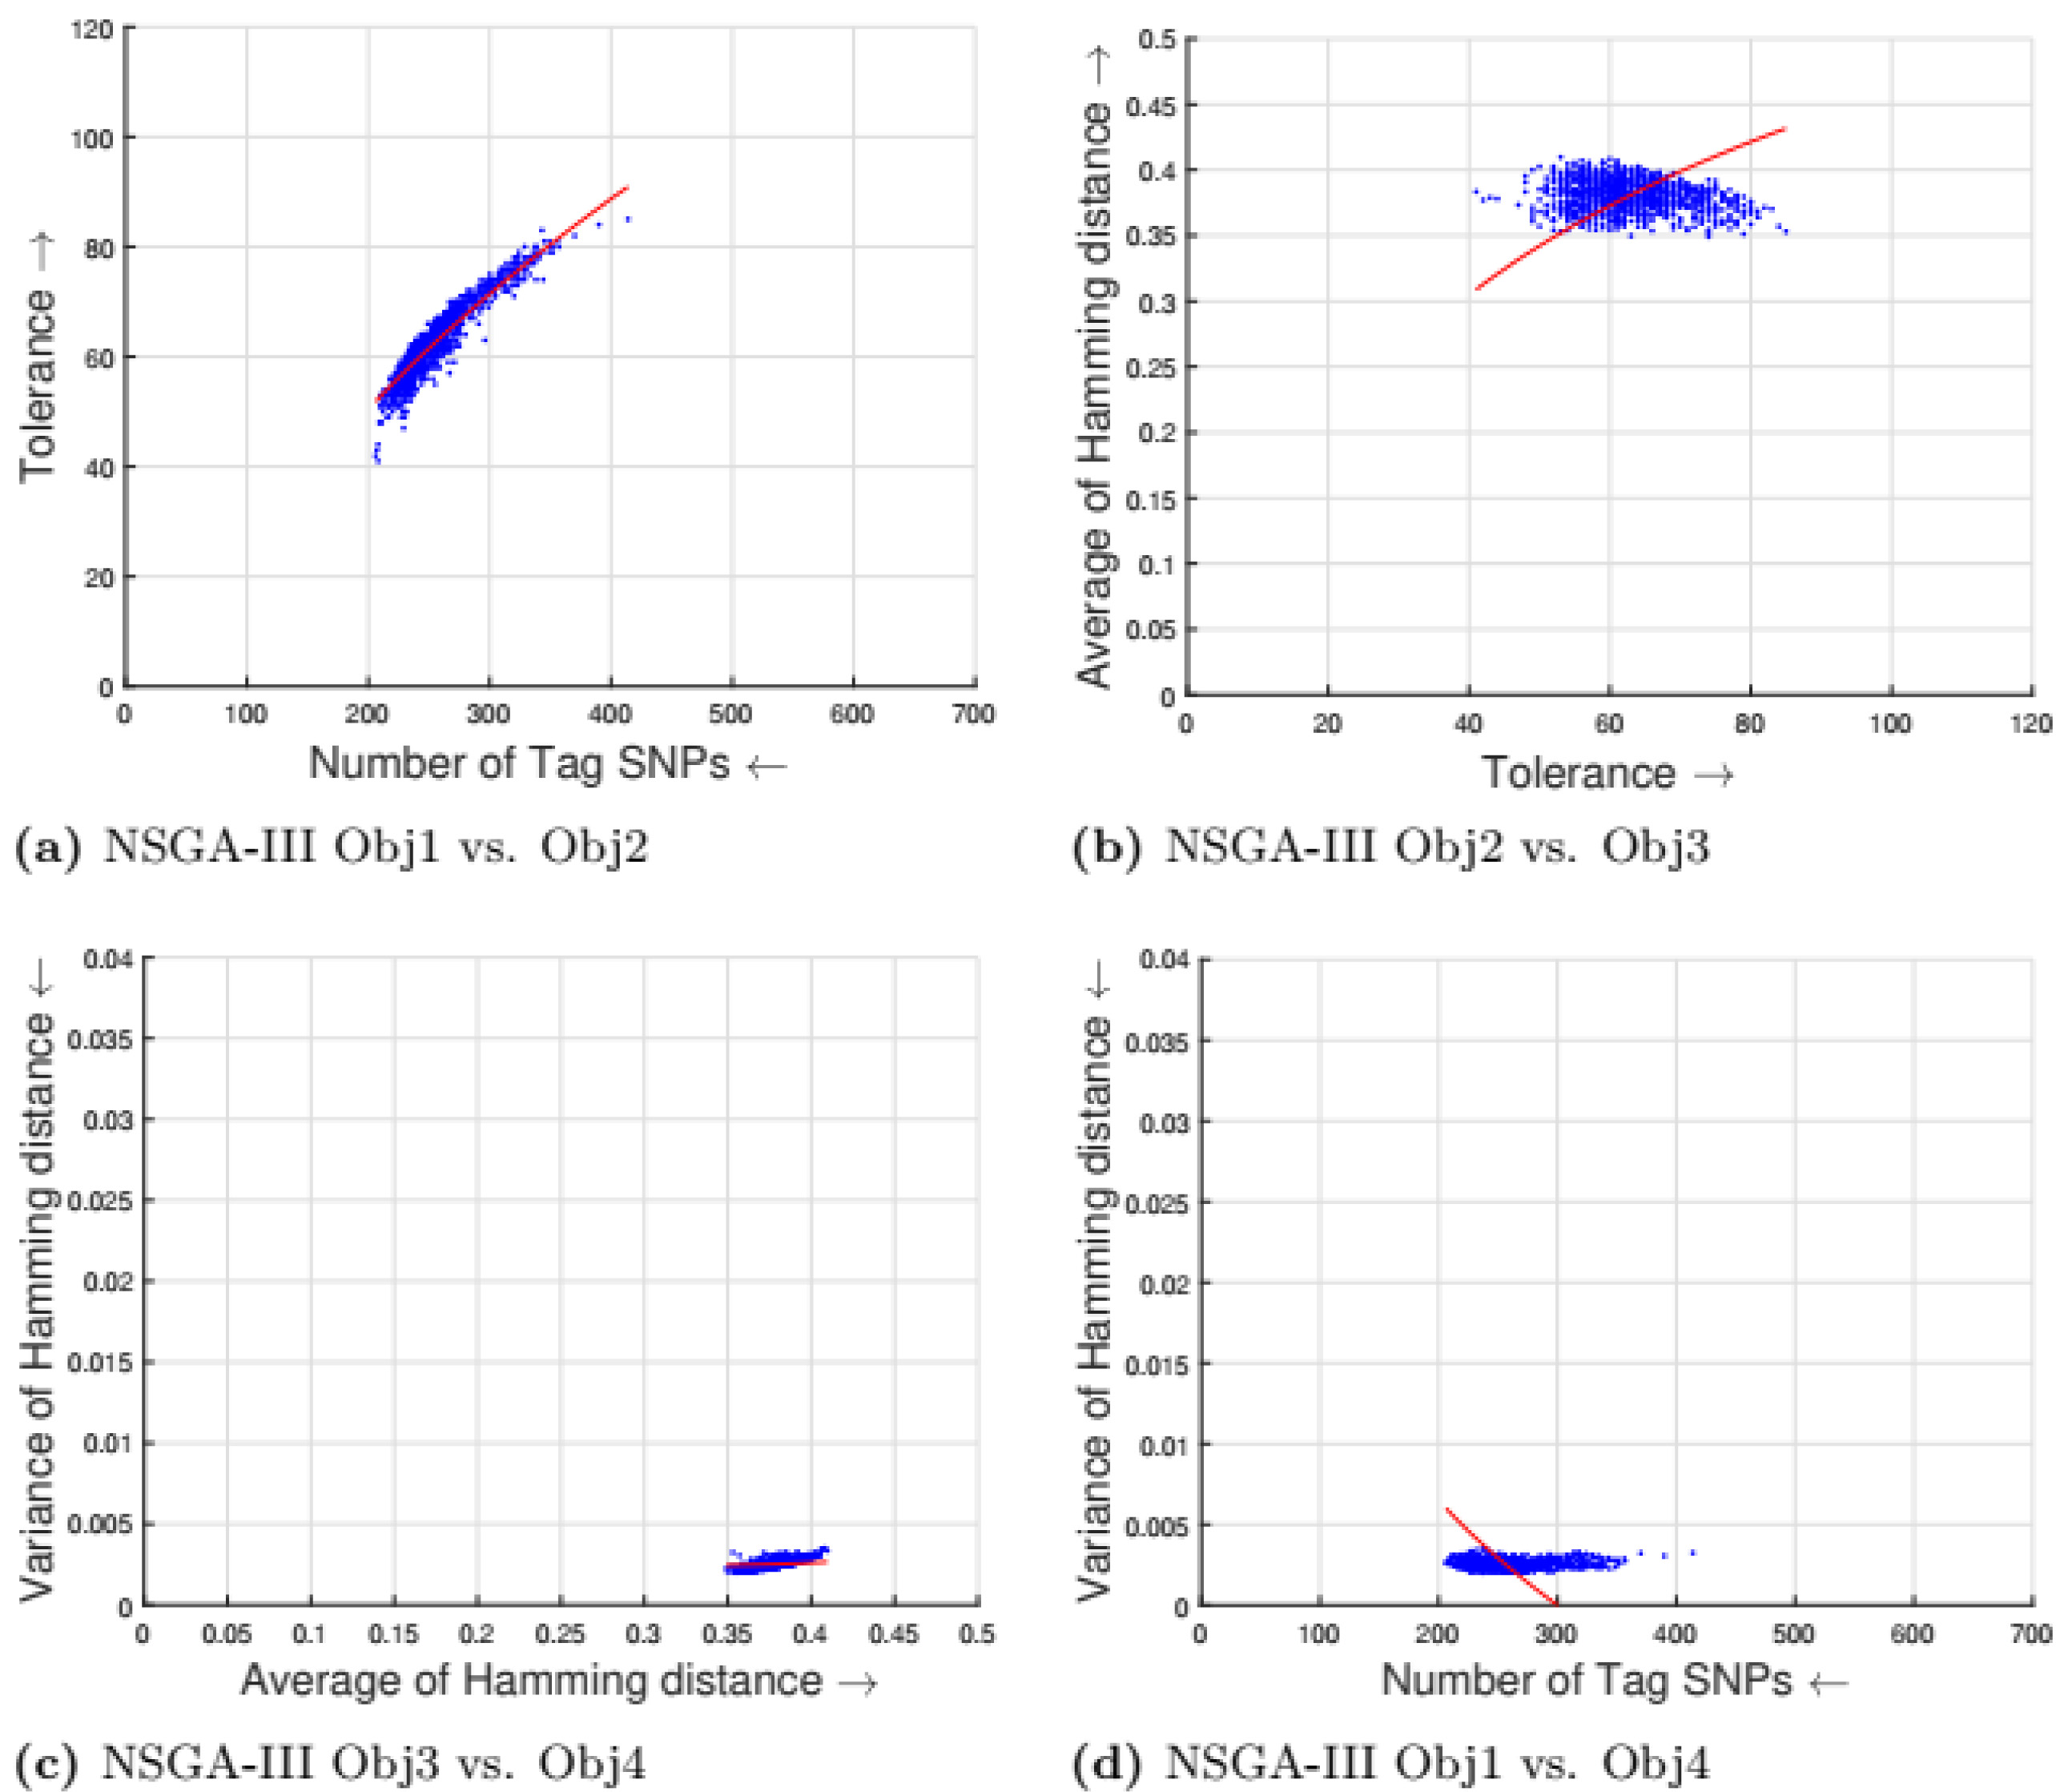
\includegraphics[width=0.28\textwidth]{analisis_assets/moqa_2022/figures/moqa_fig_nsga3_random.jpeg} &
        
\includegraphics[width=0.28\textwidth]{analisis_assets/20260430T185224/2_comparativa/1_frentes/frentes_pareto/frentes_pareto_nsga3_random_dense_full.png} &
        
\includegraphics[width=0.28\textwidth]{analisis_assets/20260430T183144/2_comparativa/1_frentes/frentes_pareto/frentes_pareto_nsga3_random_dense_full.png} \\
        Moqa & Exp. A (RD) & Exp. B (RD) \\
    \end{tabular}
    \caption{Comparativa de frentes Random para NSGA-III frente al original de Moqa.}
\end{figure}

\begin{itemize}
    \item \textbf{Similitudes:} Se aprecia una similitud notable en la disposición y densidad de las soluciones obtenidas.
    \item \textbf{Diferencias:} La comparativa no revela diferencias de peso en la configuración de los frentes.
\end{itemize}

\subsubsection{MOEA/D: Análisis de la variante PBI}

\begin{figure}[H]
    \centering
    \begin{tabular}{@{}ccccc@{}}
        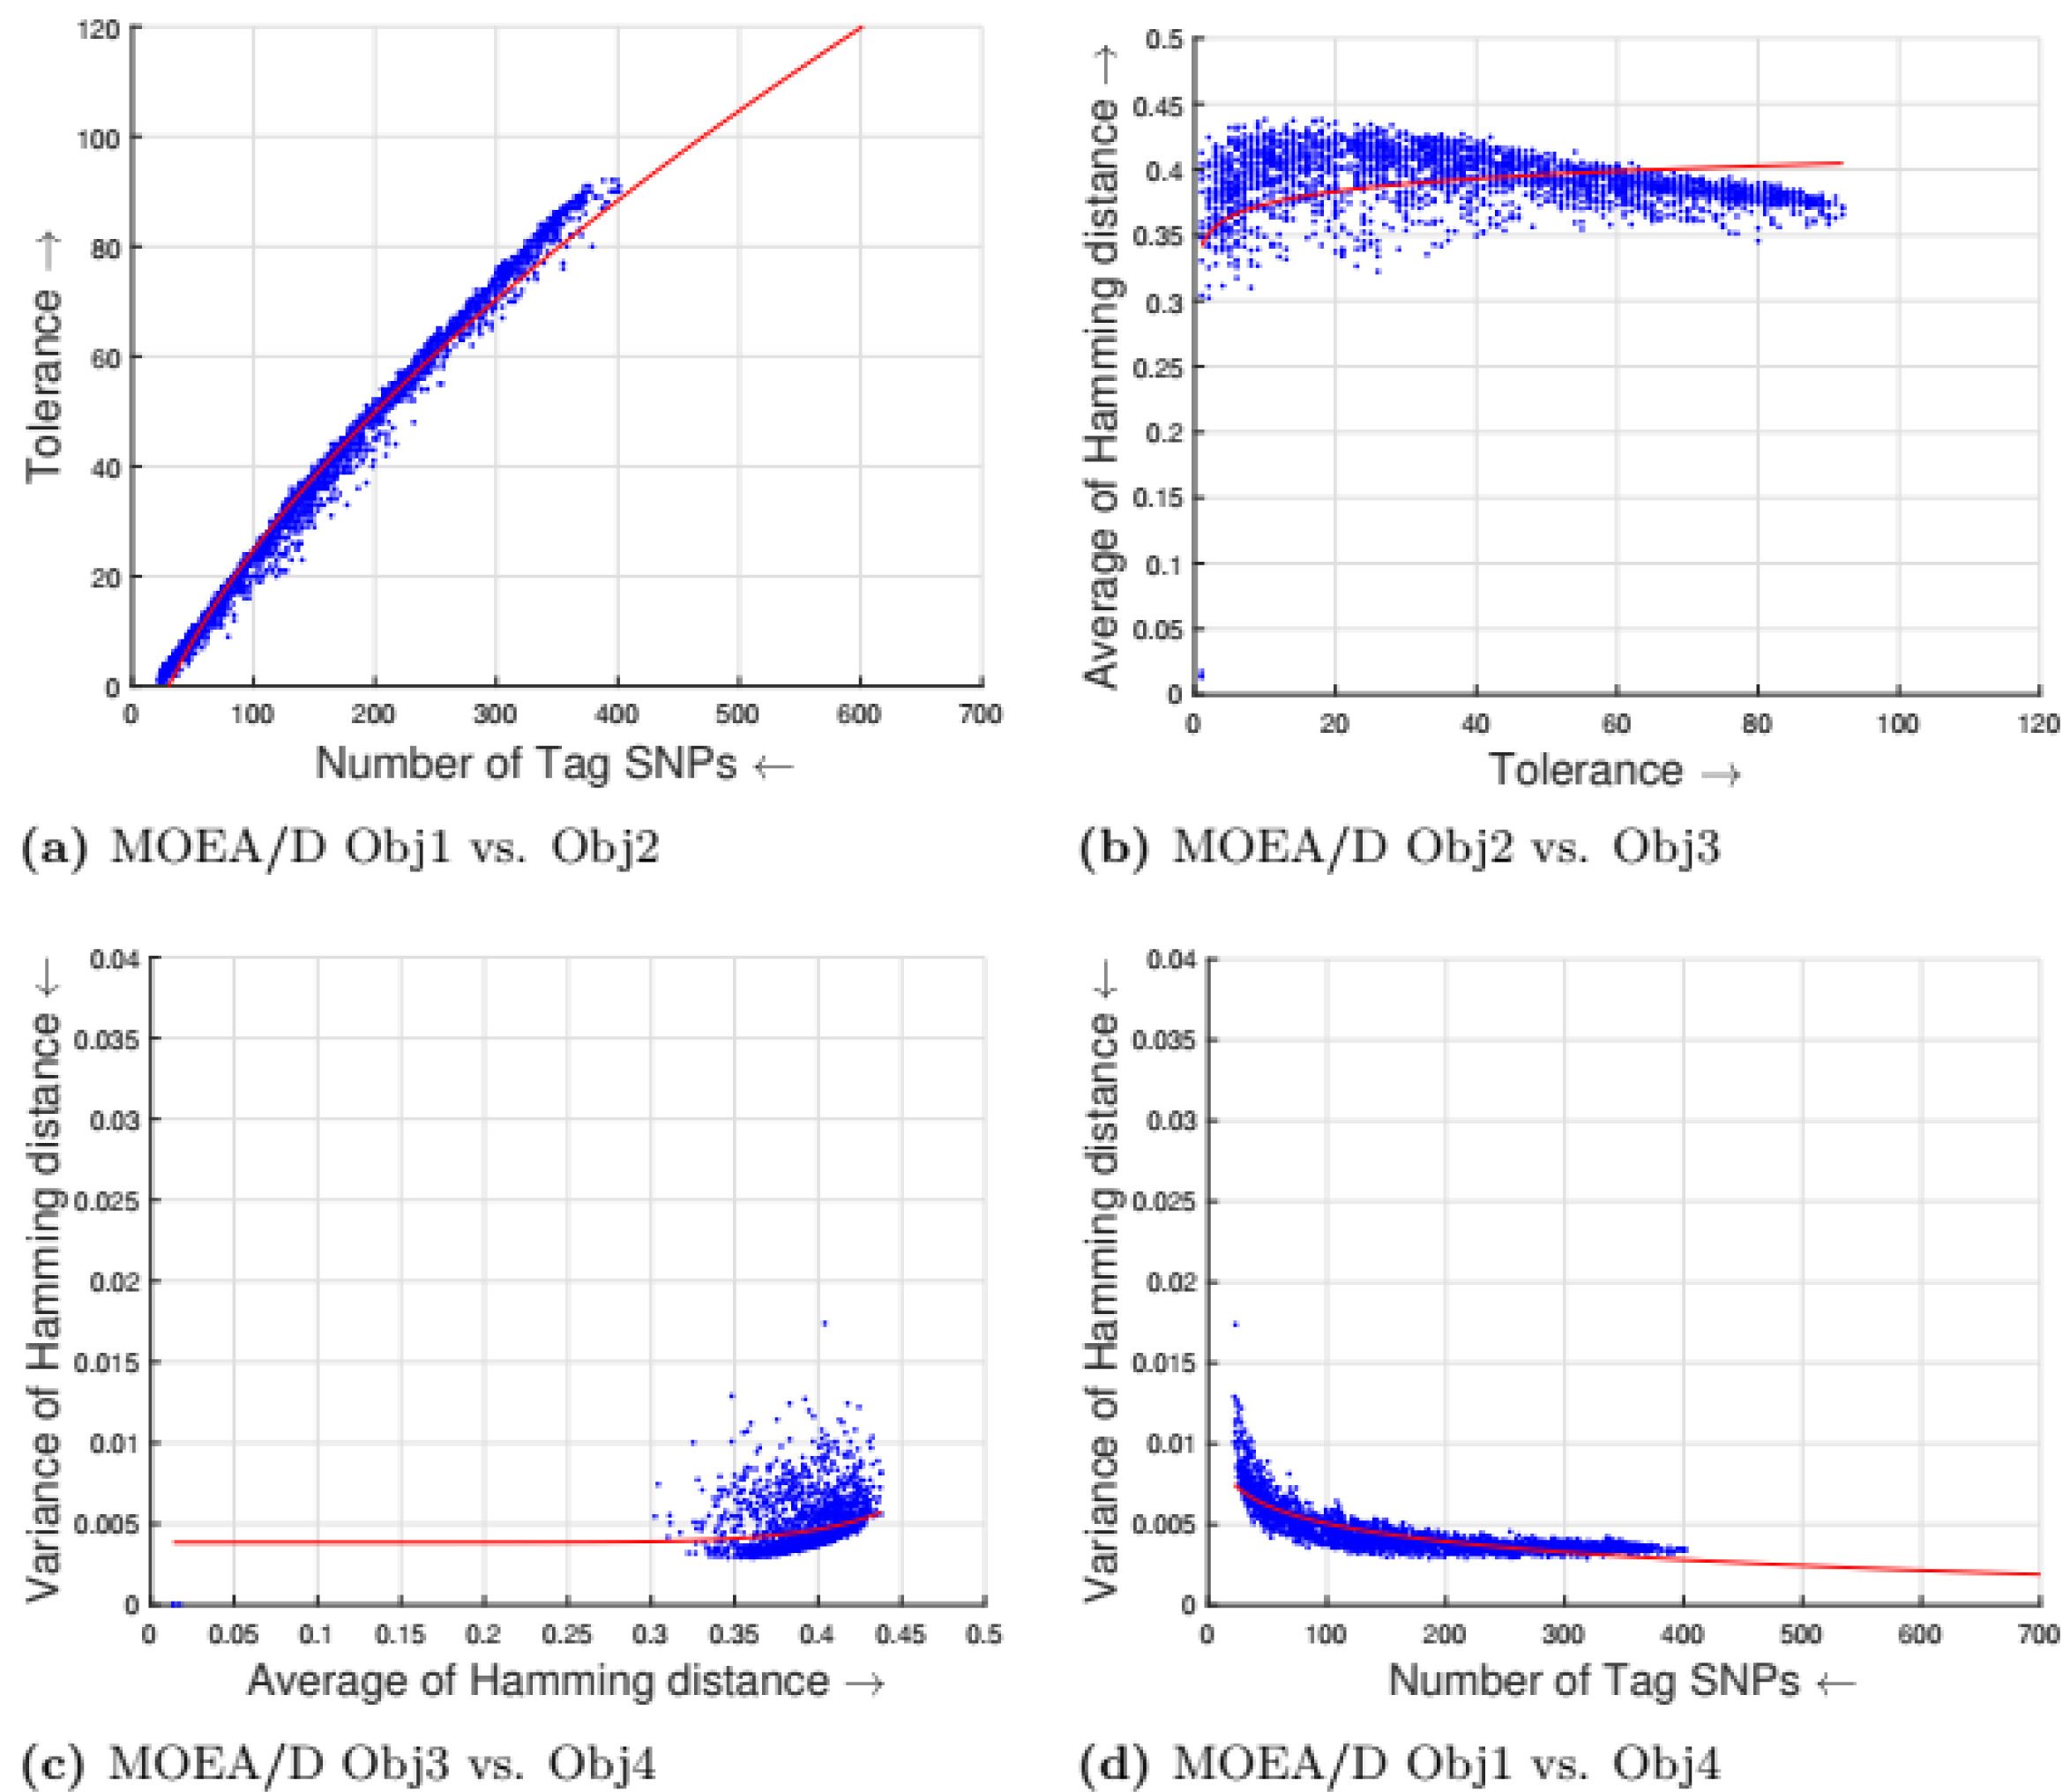
\includegraphics[width=0.18\textwidth]{analisis_assets/moqa_2022/figures/moqa_fig_moead_greedy.jpeg} &
        
\includegraphics[width=0.18\textwidth]{analisis_assets/20260430T185224/2_comparativa/1_frentes/frentes_pareto/frentes_pareto_moead_pbi_greedy_ting_full.png} &
        
\includegraphics[width=0.18\textwidth]{analisis_assets/20260430T185224/2_comparativa/1_frentes/frentes_pareto/frentes_pareto_moead_pbi_greedy_hybrid_full.png} &
        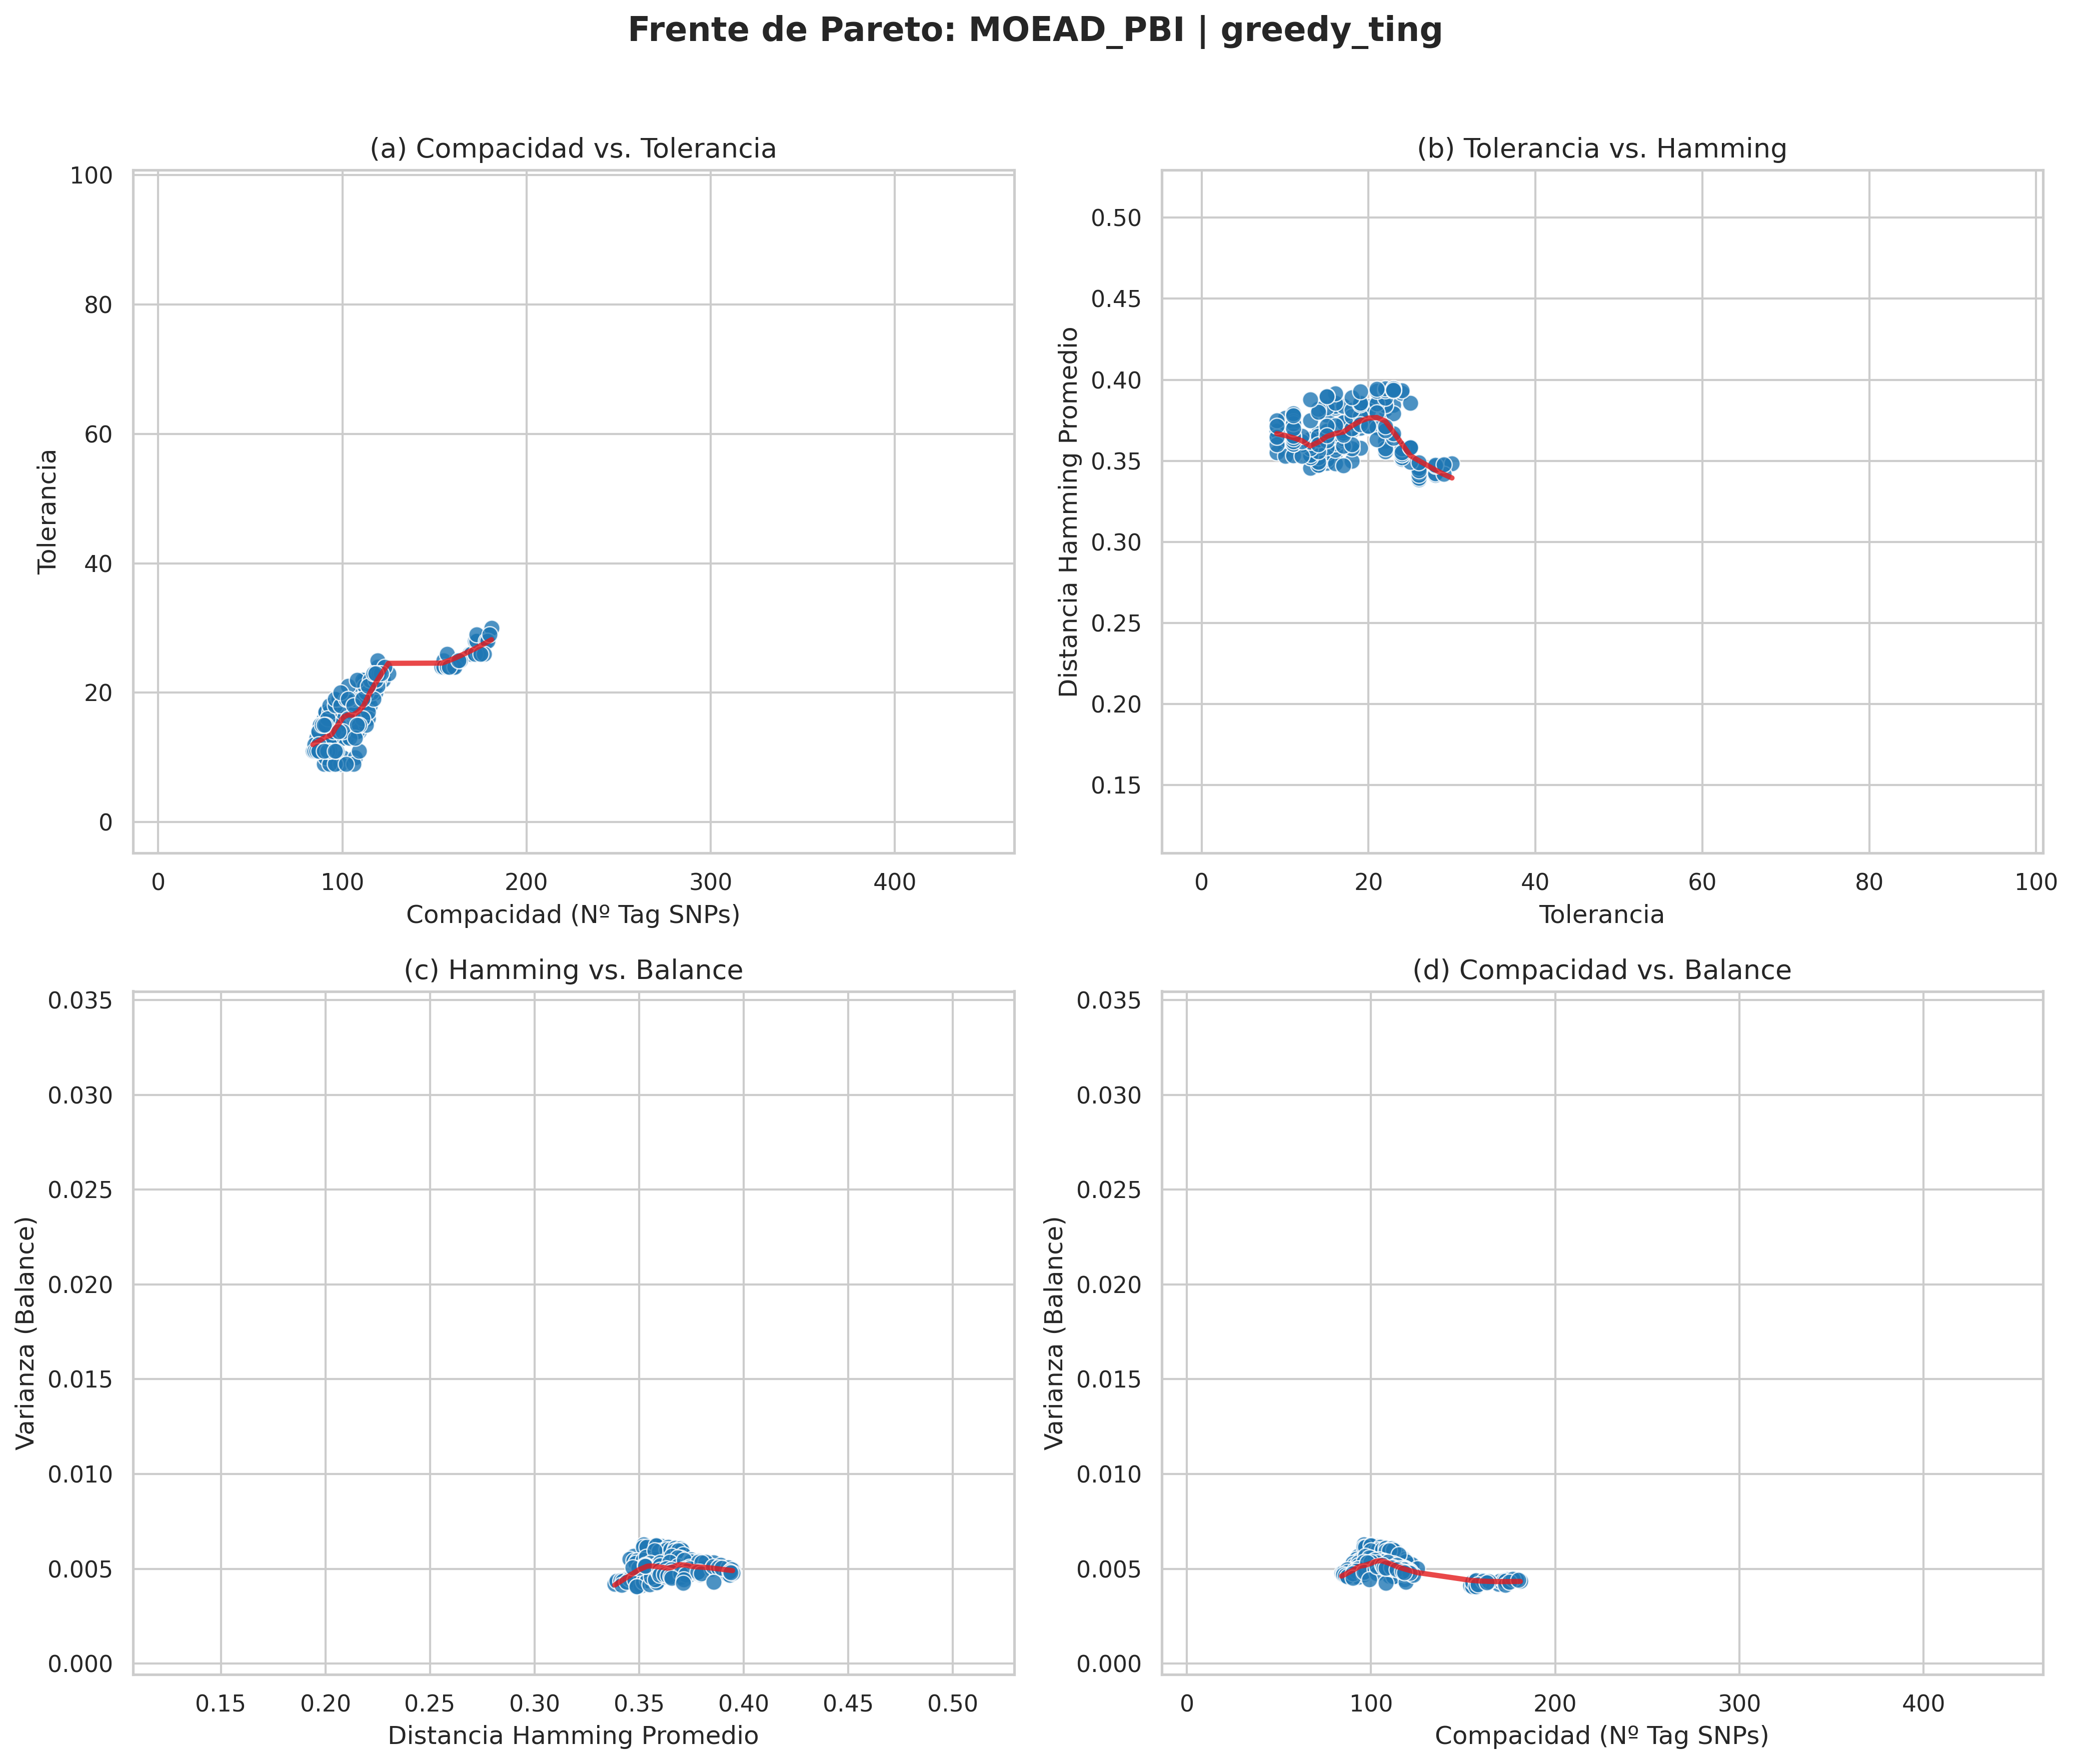
\includegraphics[width=0.18\textwidth]{analisis_assets/20260430T183144/2_comparativa/1_frentes/frentes_pareto/frentes_pareto_moead_pbi_greedy_ting_full.png} &
        
\includegraphics[width=0.18\textwidth]{analisis_assets/20260430T183144/2_comparativa/1_frentes/frentes_pareto/frentes_pareto_moead_pbi_greedy_hybrid_full.png} \\
        Moqa & Exp. A (GT) & Exp. A (GH) & Exp. B (GT) & Exp. B (GH) \\
    \end{tabular}
    \caption{Comparativa de frentes Greedy para MOEA/D-PBI frente al original de Moqa.}
\end{figure}

\begin{itemize}
    \item \textbf{Similitudes:} Se observa una morfología comparable entre el frente de Moqa y el obtenido en la ejecución A.
    \item \textbf{Diferencias:} Se aprecia un contraste claro entre Moqa/A y la ejecución B, cuyos frentes aparecen mucho más comprimidos.
\end{itemize}

\begin{figure}[H]
    \centering
    \begin{tabular}{@{}ccc@{}}
        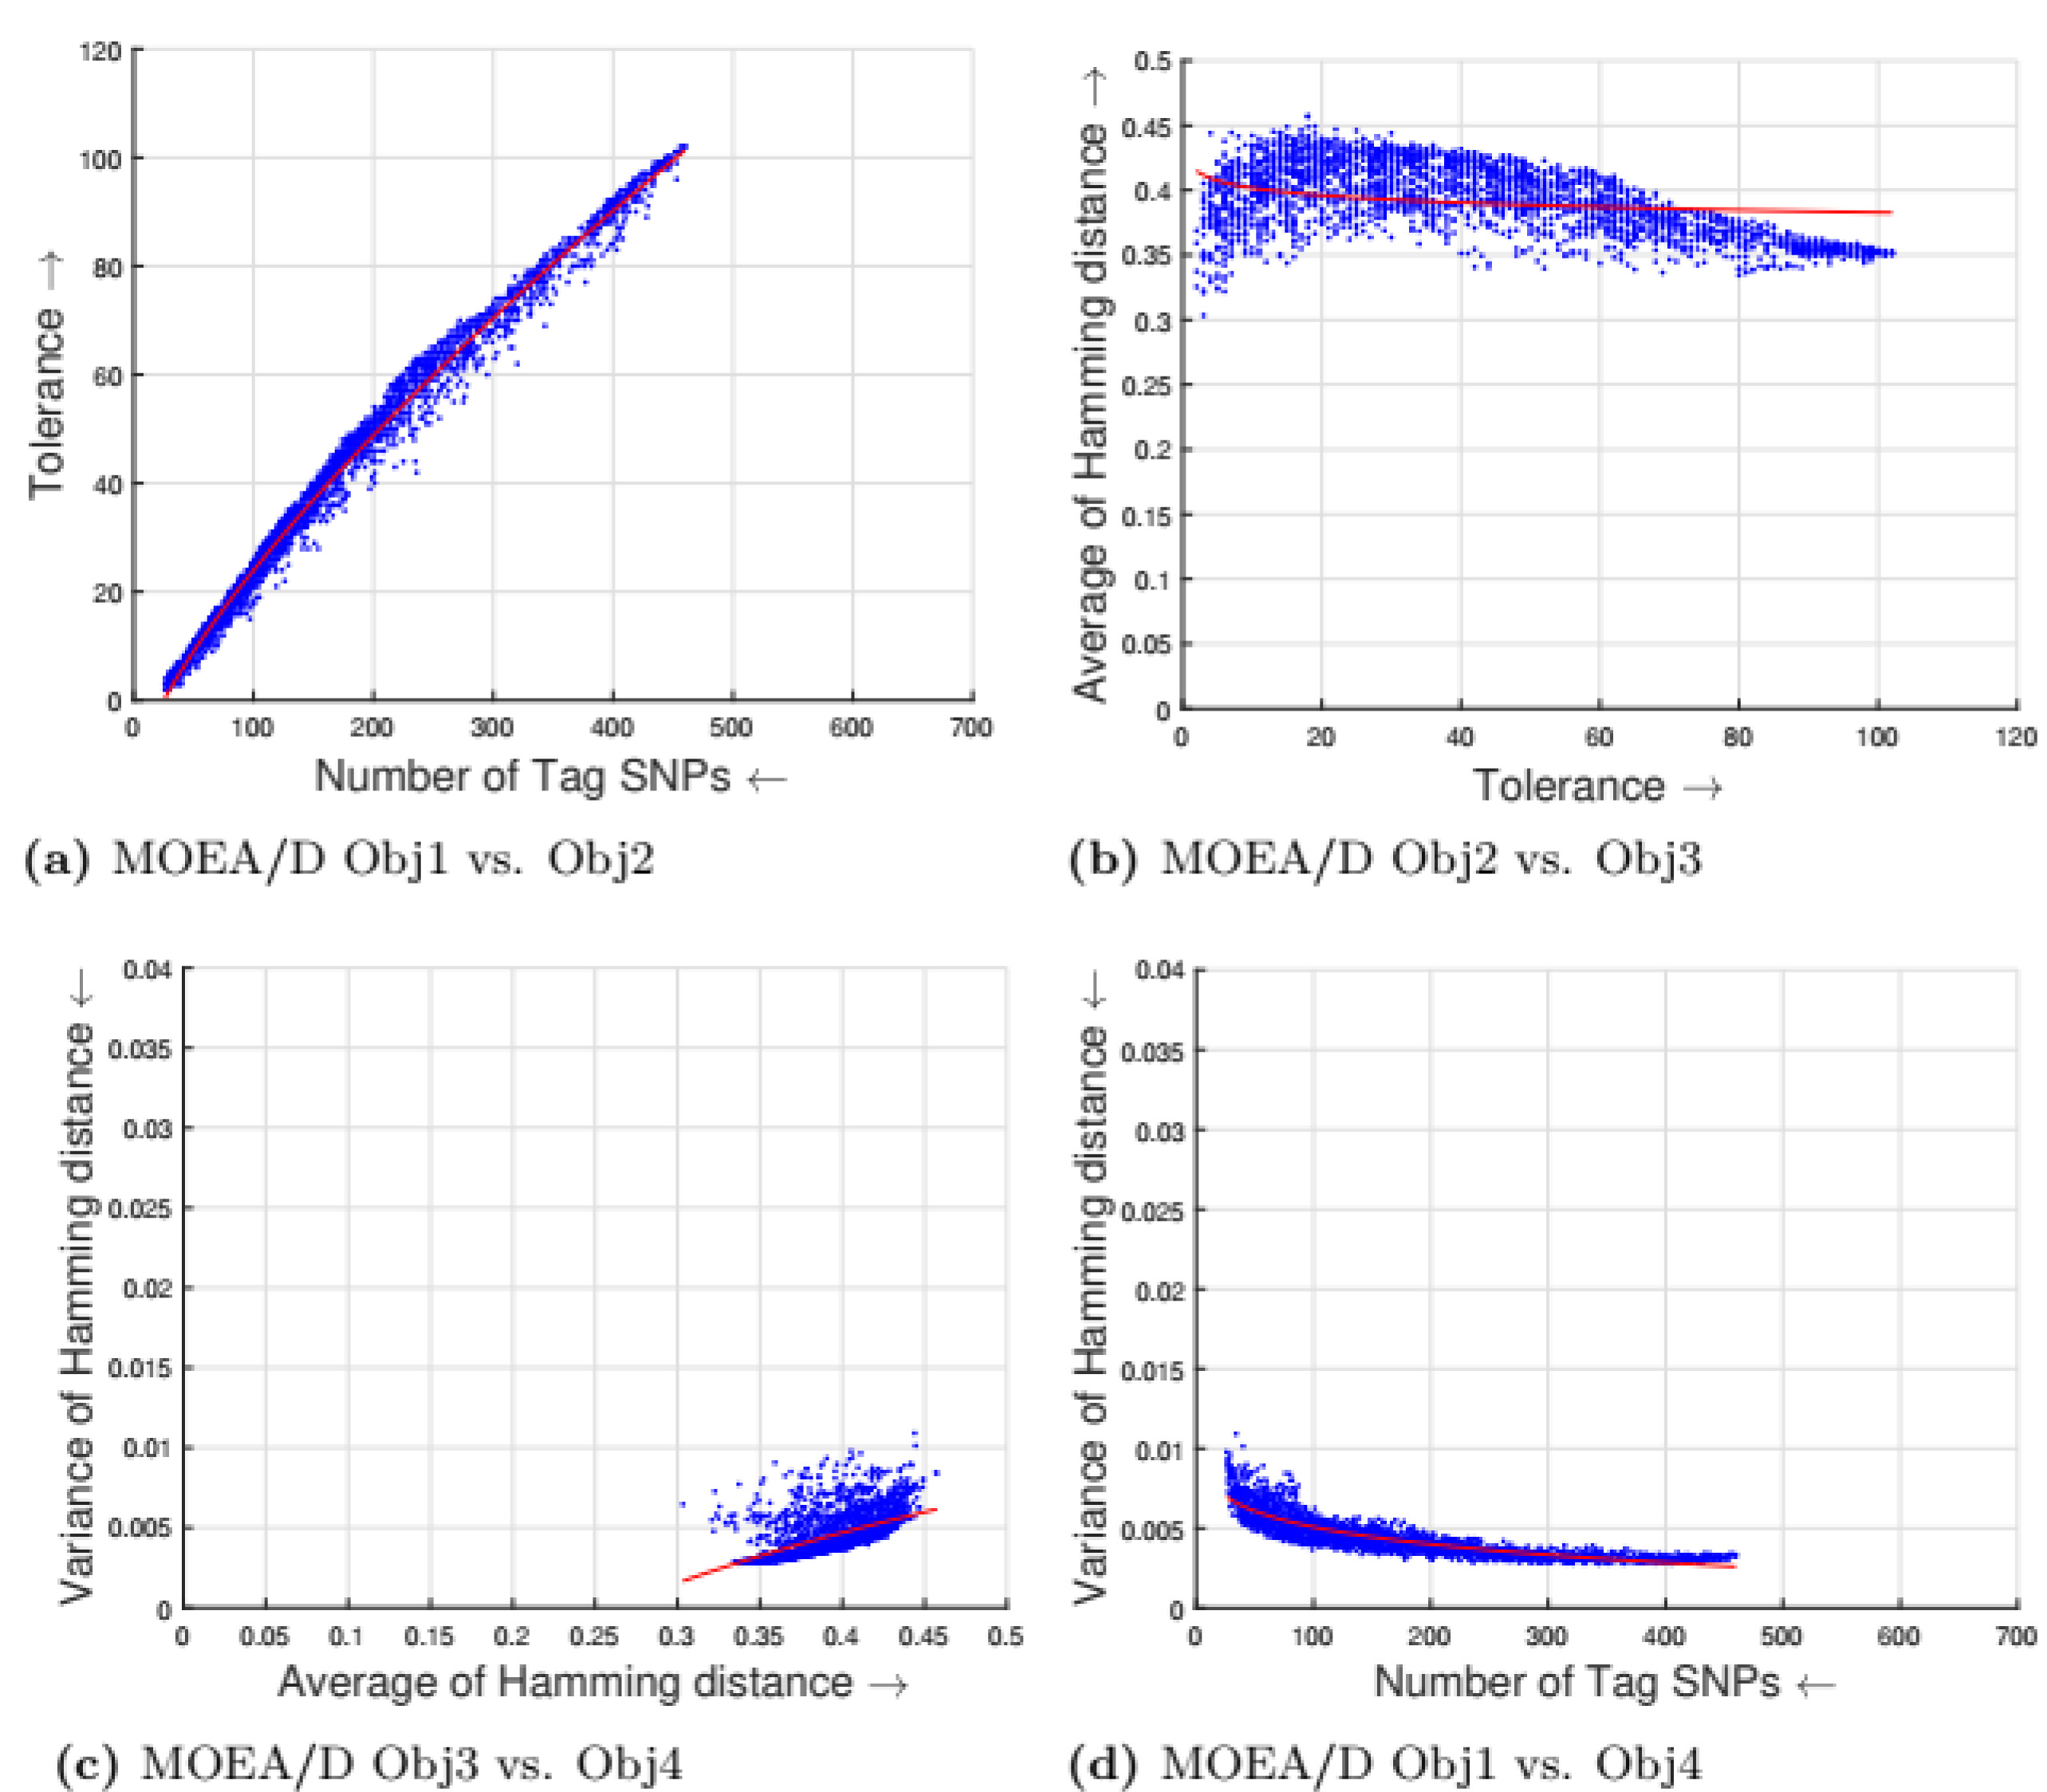
\includegraphics[width=0.28\textwidth]{analisis_assets/moqa_2022/figures/moqa_fig_moead_random.jpeg} &
        
\includegraphics[width=0.28\textwidth]{analisis_assets/20260430T185224/2_comparativa/1_frentes/frentes_pareto/frentes_pareto_moead_pbi_random_dense_full.png} &
        
\includegraphics[width=0.28\textwidth]{analisis_assets/20260430T183144/2_comparativa/1_frentes/frentes_pareto/frentes_pareto_moead_pbi_random_dense_full.png} \\
        Moqa & Exp. A (RD) & Exp. B (RD) \\
    \end{tabular}
    \caption{Comparativa de frentes Random para MOEA/D-PBI frente al original de Moqa.}
\end{figure}

\begin{itemize}
    \item \textbf{Similitudes:} La correspondencia visual entre las ejecuciones realizadas y los resultados de Moqa es bastante reducida.
    \item \textbf{Diferencias:} Los frentes obtenidos en A y B muestran menos dispersión y aparecen mucho más compactos que los reportados en el estudio original.
\end{itemize}

\subsubsection{MOEA/D: Análisis de la variante Tchebycheff (TCHE)}

\begin{figure}[H]
    \centering
    \begin{tabular}{@{}ccccc@{}}
        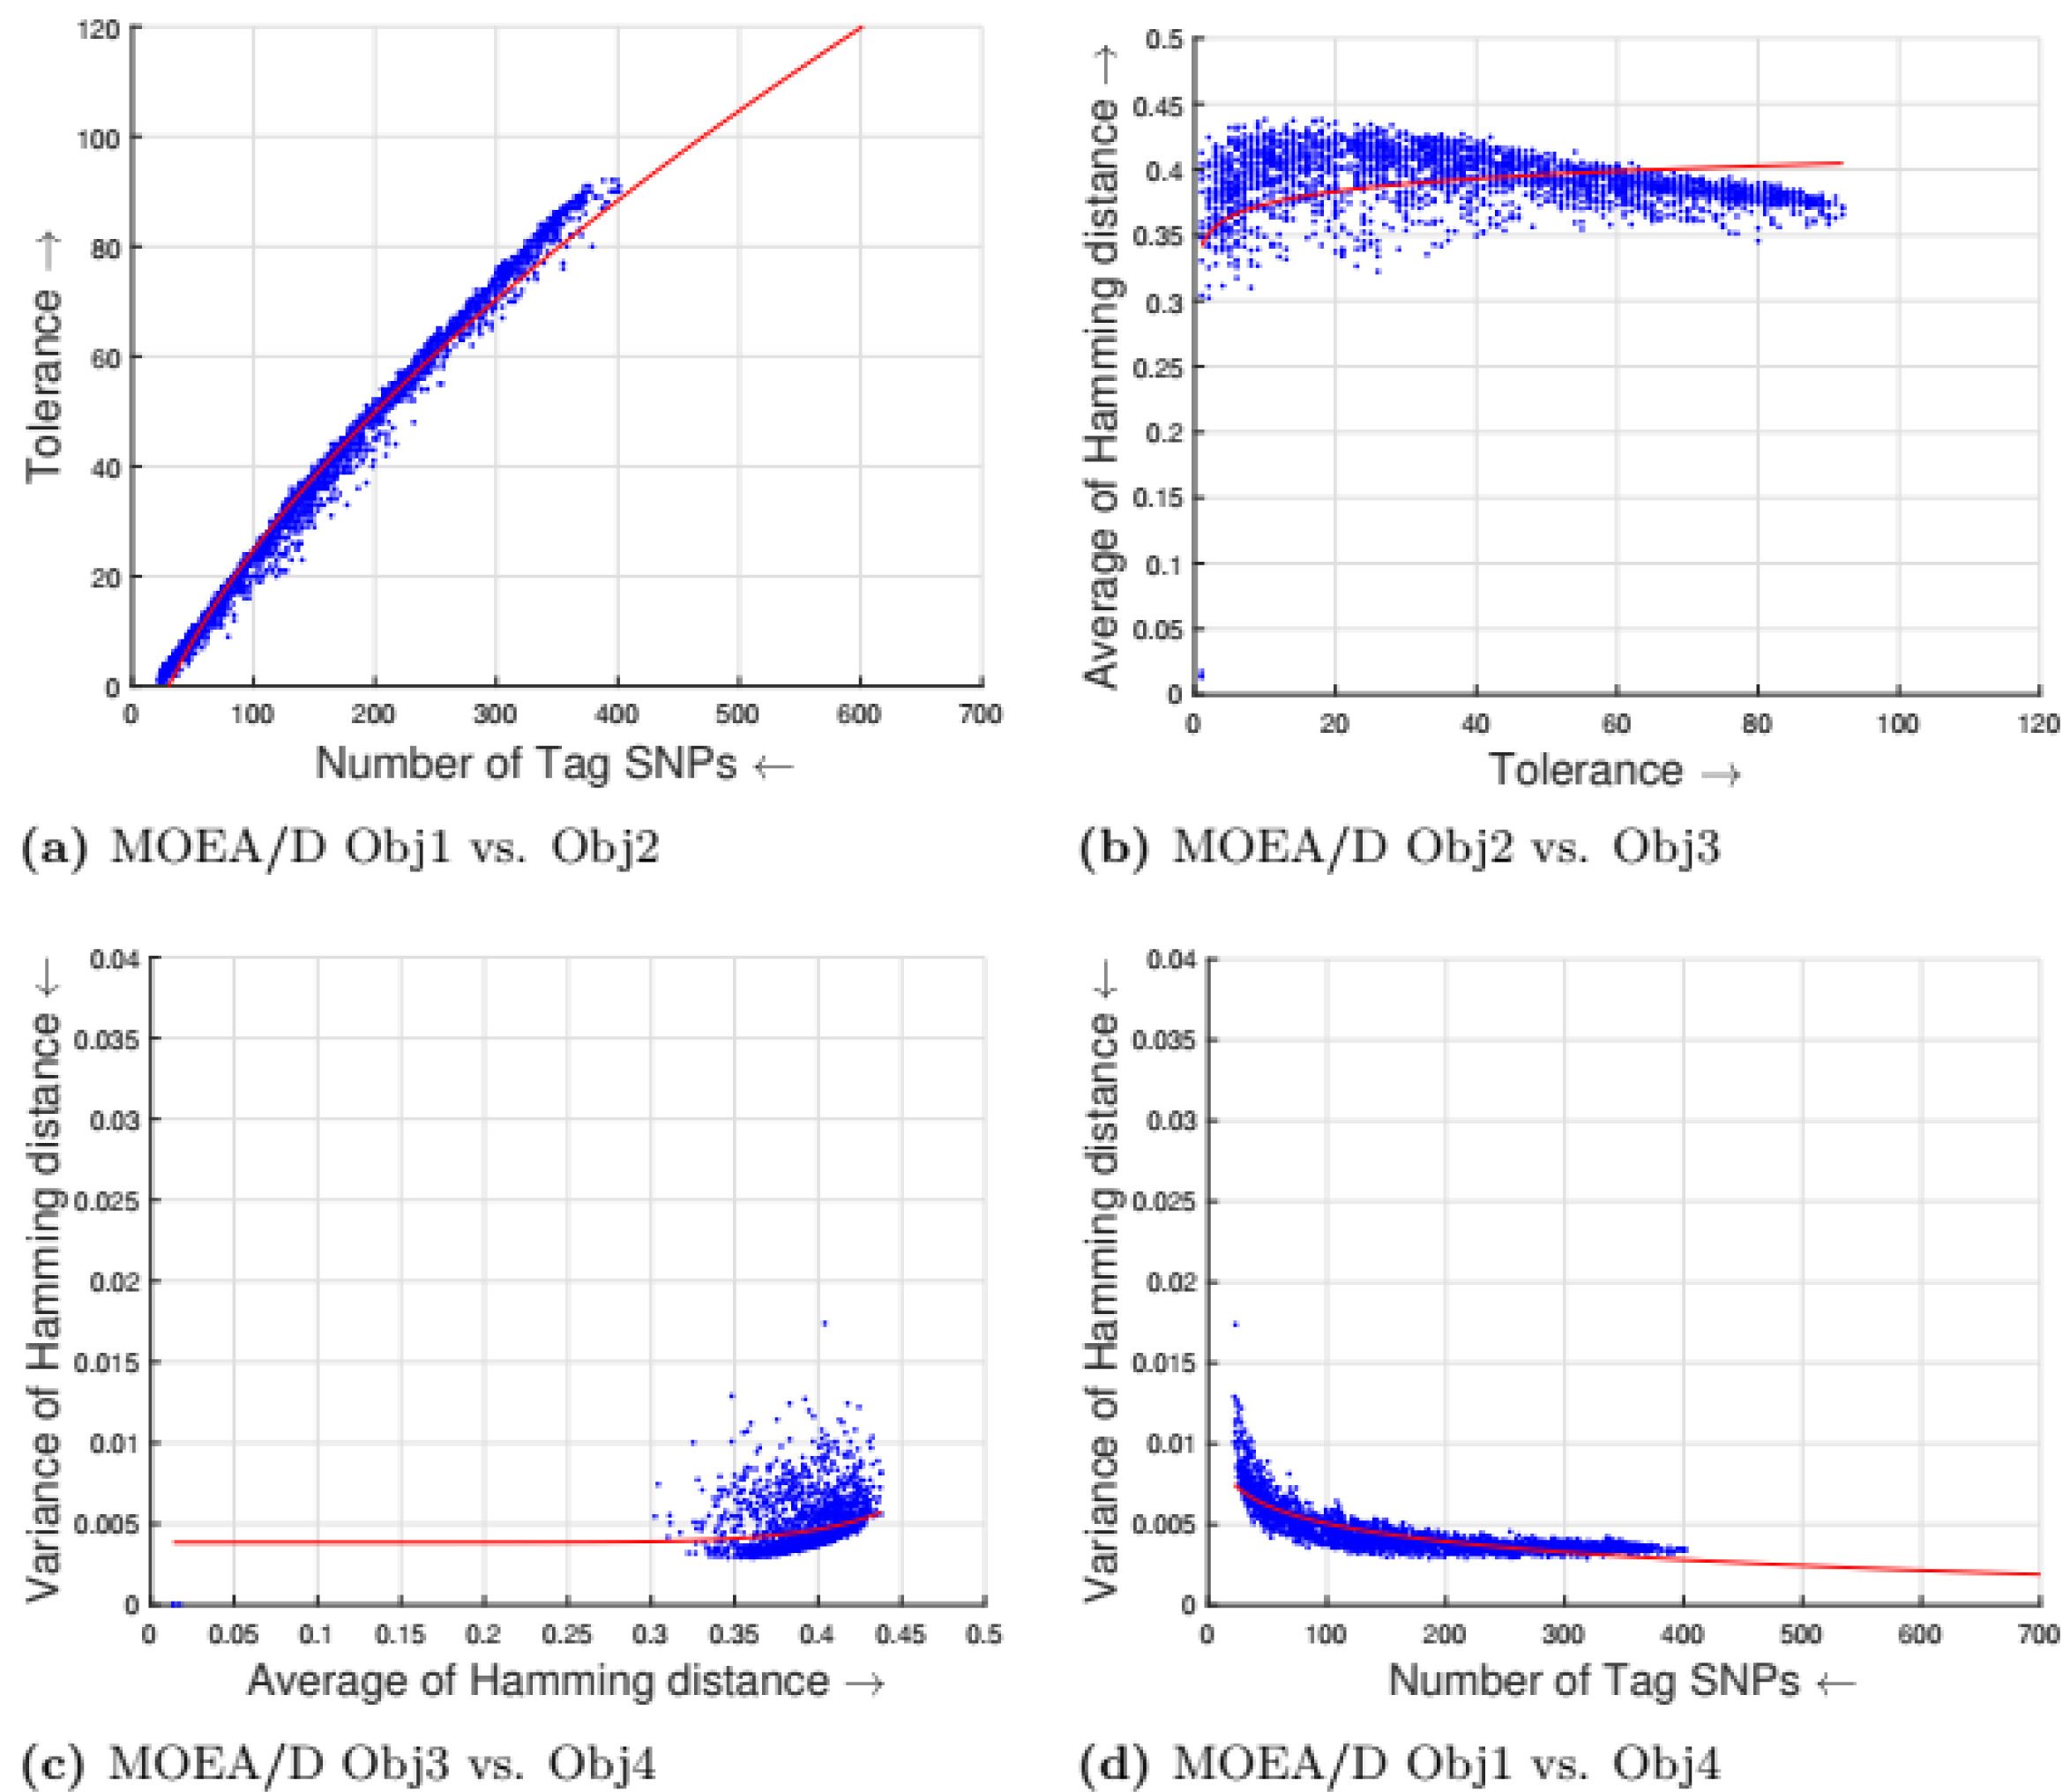
\includegraphics[width=0.18\textwidth]{analisis_assets/moqa_2022/figures/moqa_fig_moead_greedy.jpeg} &
        
\includegraphics[width=0.18\textwidth]{analisis_assets/20260430T185224/2_comparativa/1_frentes/frentes_pareto/frentes_pareto_moead_tche_greedy_ting_full.png} &
        
\includegraphics[width=0.18\textwidth]{analisis_assets/20260430T185224/2_comparativa/1_frentes/frentes_pareto/frentes_pareto_moead_tche_greedy_hybrid_full.png} &
        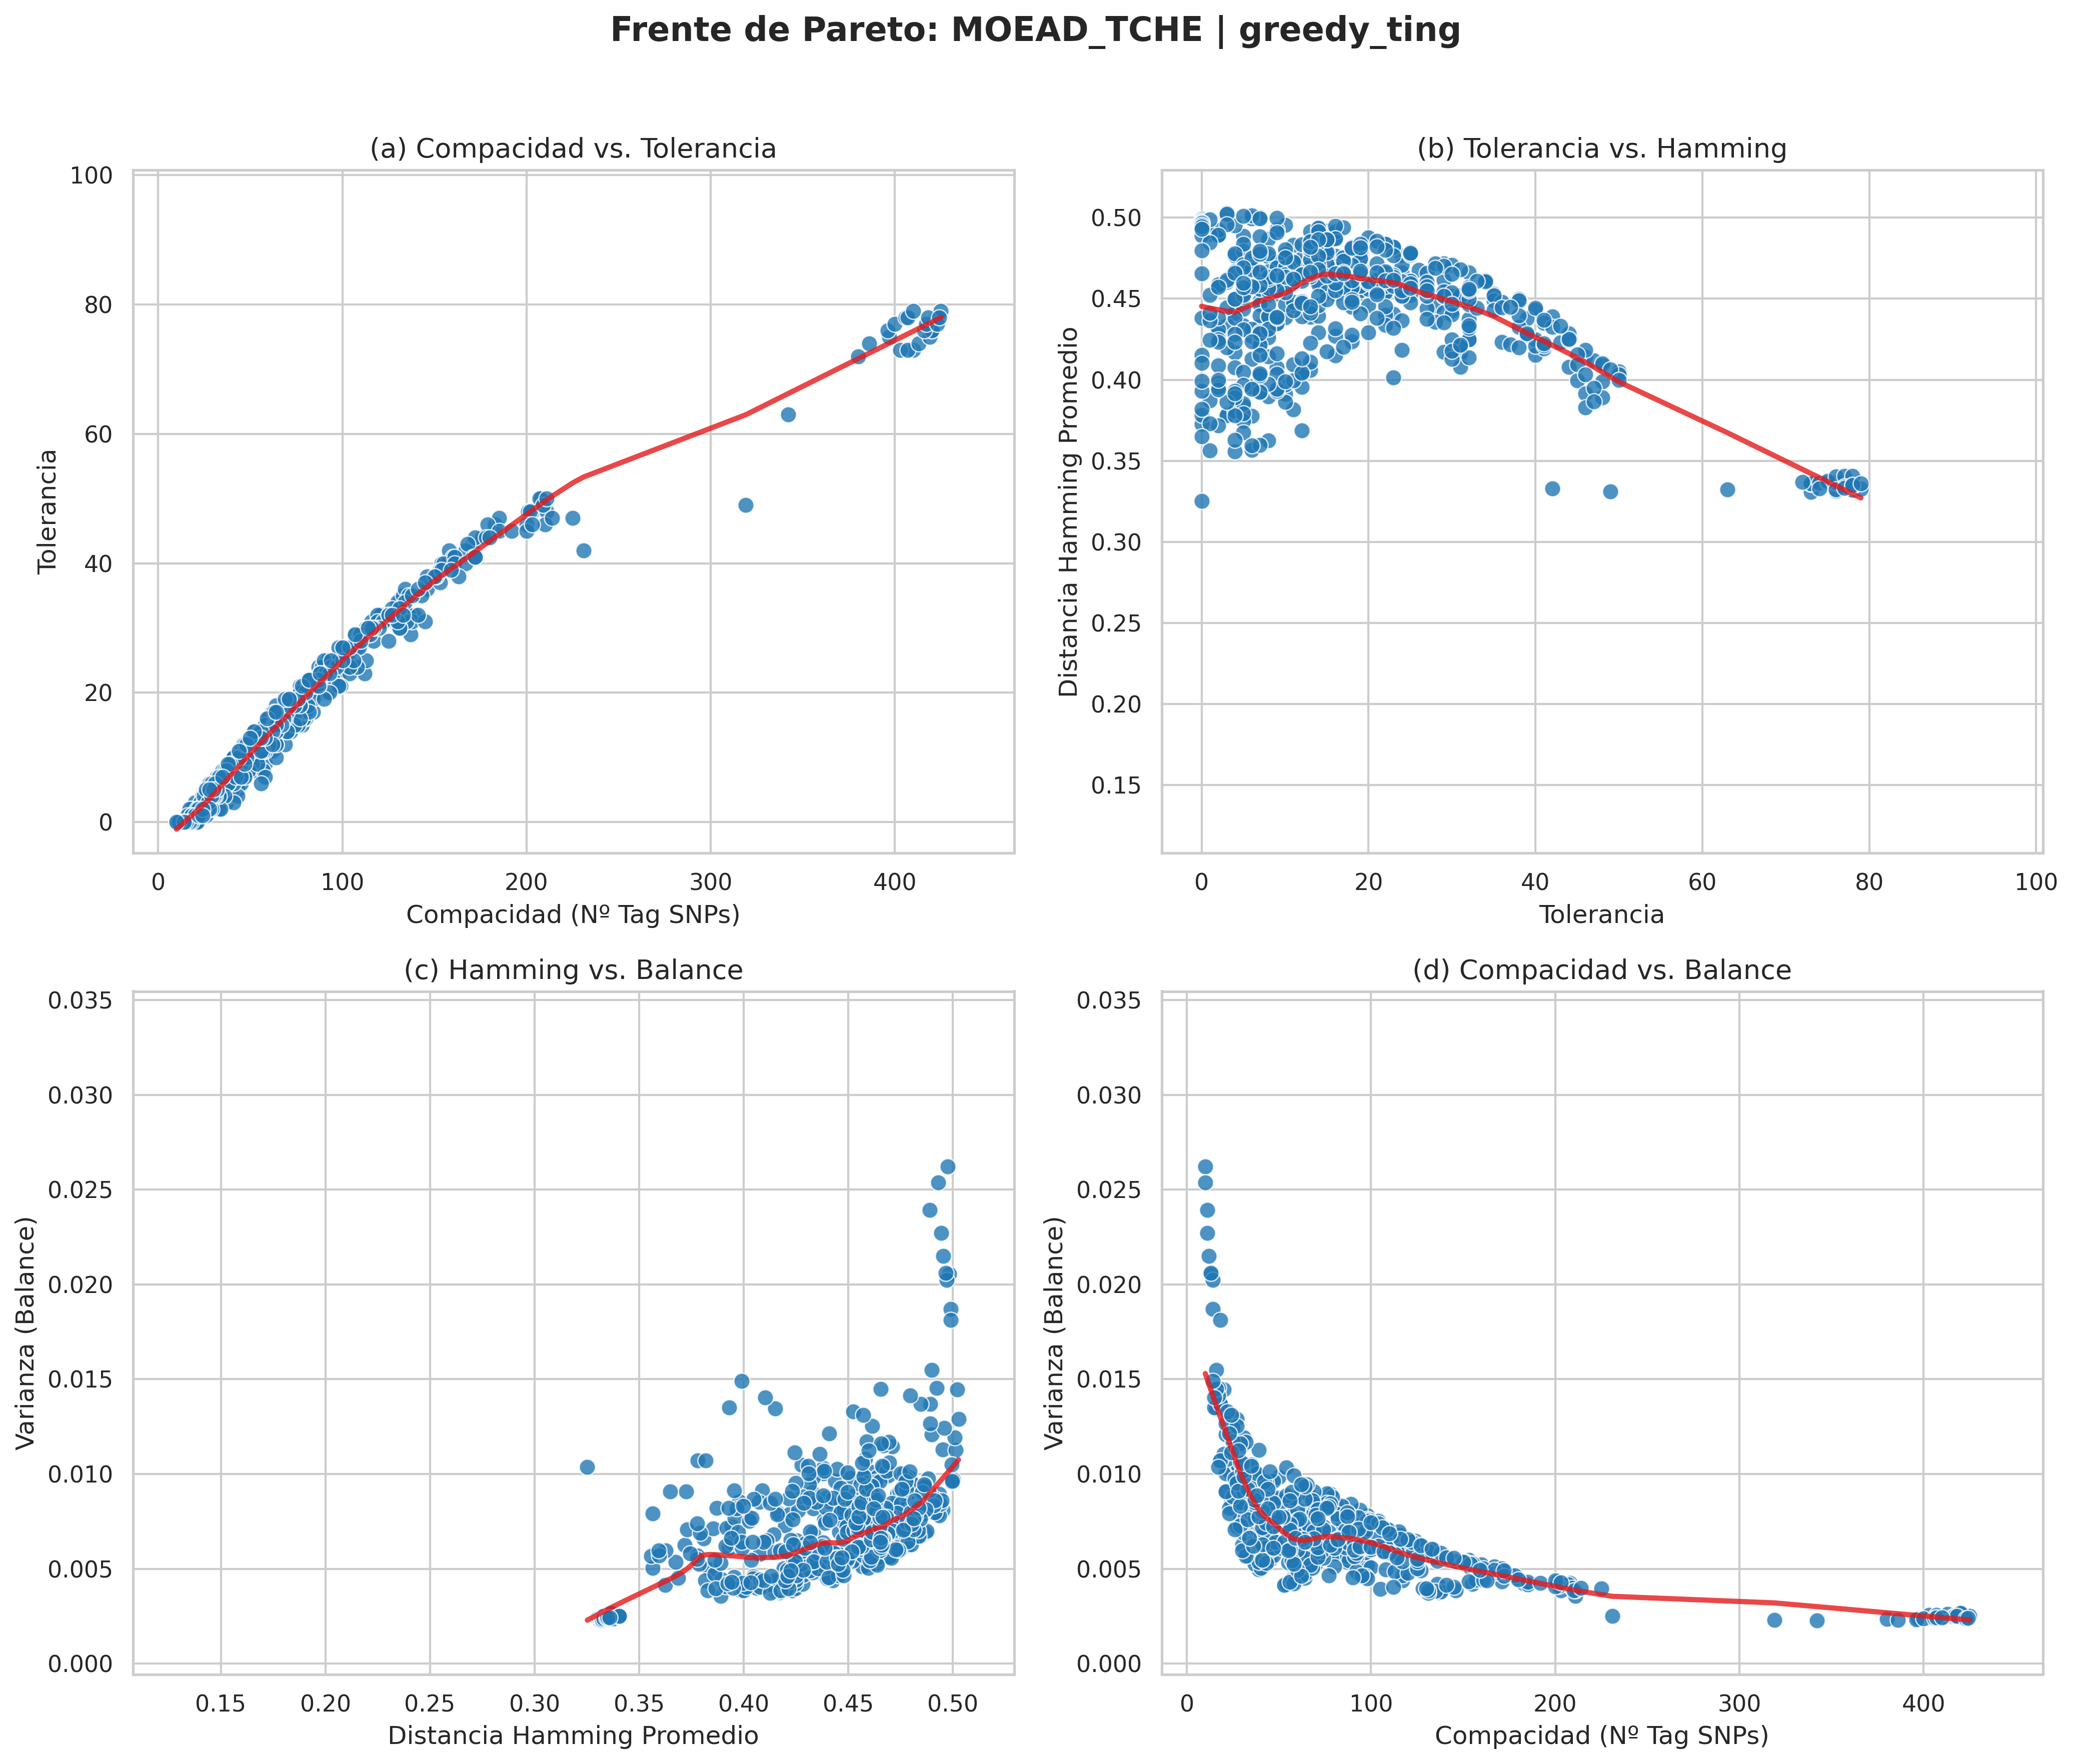
\includegraphics[width=0.18\textwidth]{analisis_assets/20260430T183144/2_comparativa/1_frentes/frentes_pareto/frentes_pareto_moead_tche_greedy_ting_full.png} &
        
\includegraphics[width=0.18\textwidth]{analisis_assets/20260430T183144/2_comparativa/1_frentes/frentes_pareto/frentes_pareto_moead_tche_greedy_hybrid_full.png} \\
        Moqa & Exp. A (GT) & Exp. A (GH) & Exp. B (GT) & Exp. B (GH) \\
    \end{tabular}
    \caption{Comparativa de frentes Greedy para MOEA/D-TCHE frente al original de Moqa.}
\end{figure}

\begin{itemize}
    \item \textbf{Similitudes:} En términos generales, se aprecian frentes con una estructura y distribución de puntos muy parecida.
    \item \textbf{Diferencias:} No se detectan variaciones morfológicas de relevancia.
\end{itemize}

\begin{figure}[H]
    \centering
    \begin{tabular}{@{}ccc@{}}
        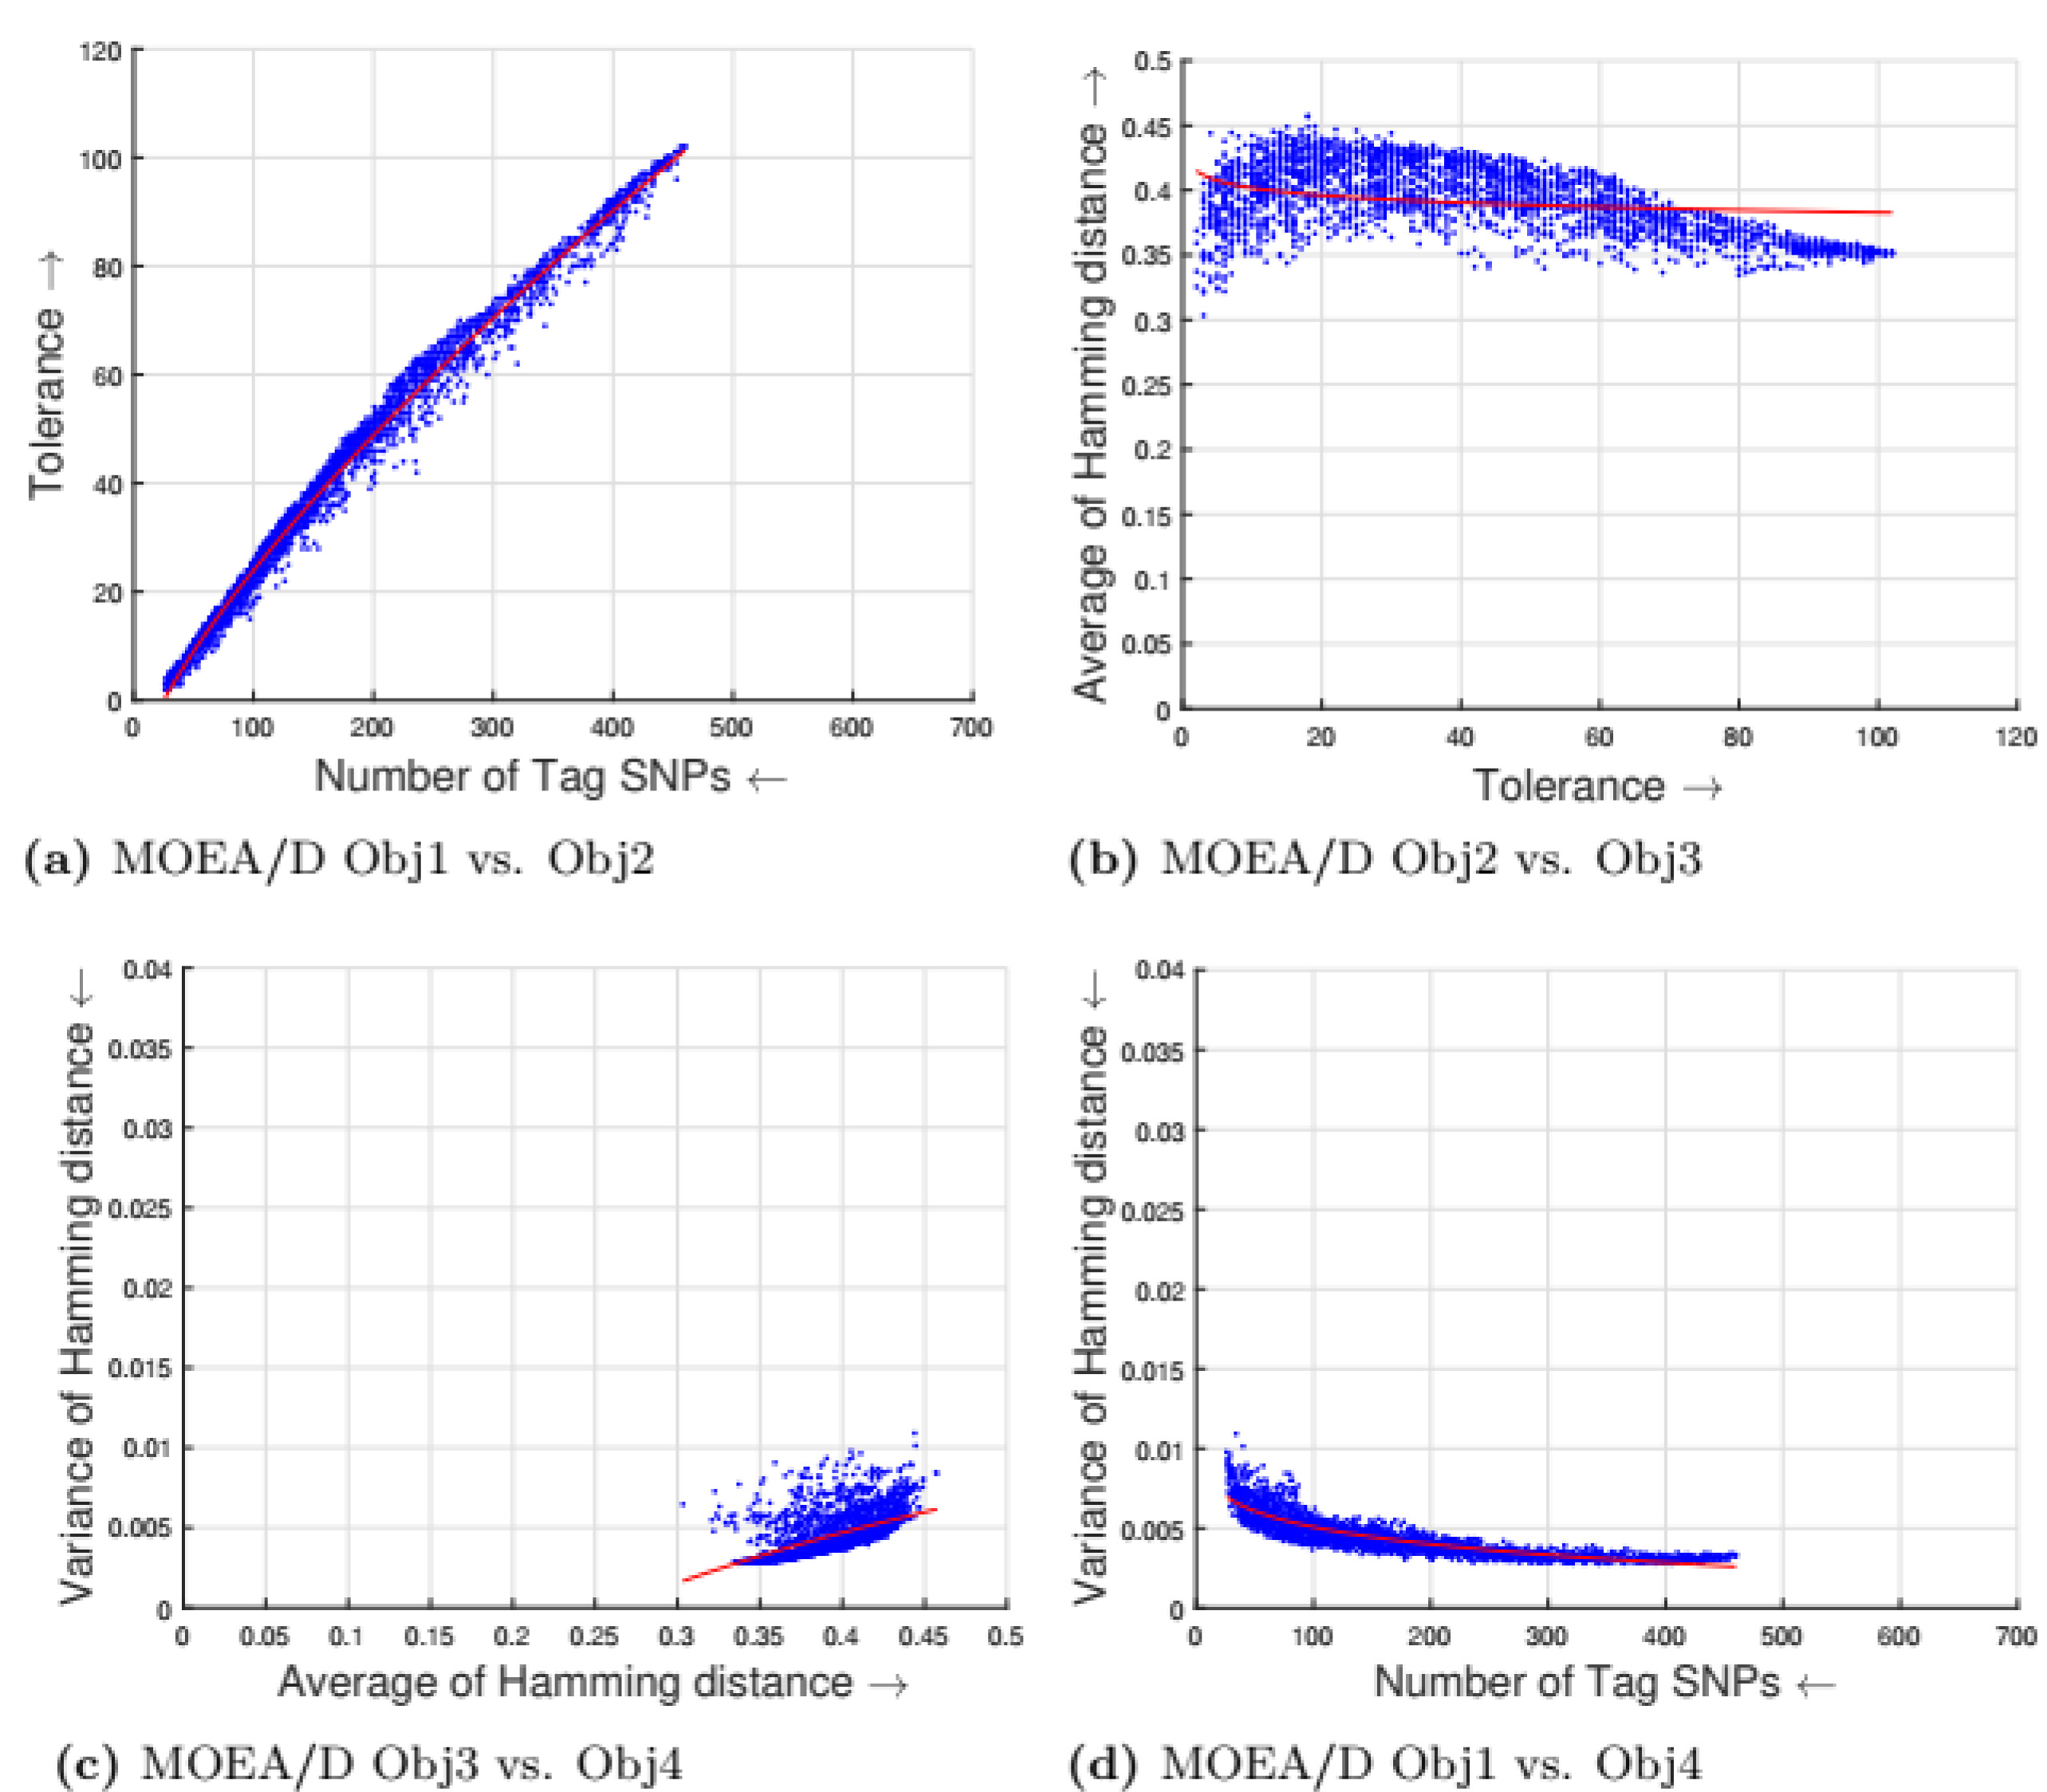
\includegraphics[width=0.28\textwidth]{analisis_assets/moqa_2022/figures/moqa_fig_moead_random.jpeg} &
        
\includegraphics[width=0.28\textwidth]{analisis_assets/20260430T185224/2_comparativa/1_frentes/frentes_pareto/frentes_pareto_moead_tche_random_dense_full.png} &
        
\includegraphics[width=0.28\textwidth]{analisis_assets/20260430T183144/2_comparativa/1_frentes/frentes_pareto/frentes_pareto_moead_tche_random_dense_full.png} \\
        Moqa & Exp. A (RD) & Exp. B (RD) \\
    \end{tabular}
    \caption{Comparativa de frentes Random para MOEA/D-TCHE frente al original de Moqa.}
\end{figure}

\begin{itemize}
    \item \textbf{Similitudes:} Las líneas de tendencia suavizadas (LOWESS) muestran un comportamiento muy parecido entre los distintos experimentos.
    \item \textbf{Diferencias:} Los frentes de referencia de Moqa parecen tener una mayor extensión espacial que los obtenidos en A y B.
\end{itemize}

\subsubsection{MOEA/D: Análisis de la variante Weighted Sum (WS)}

\begin{figure}[H]
    \centering
    \begin{tabular}{@{}ccccc@{}}
        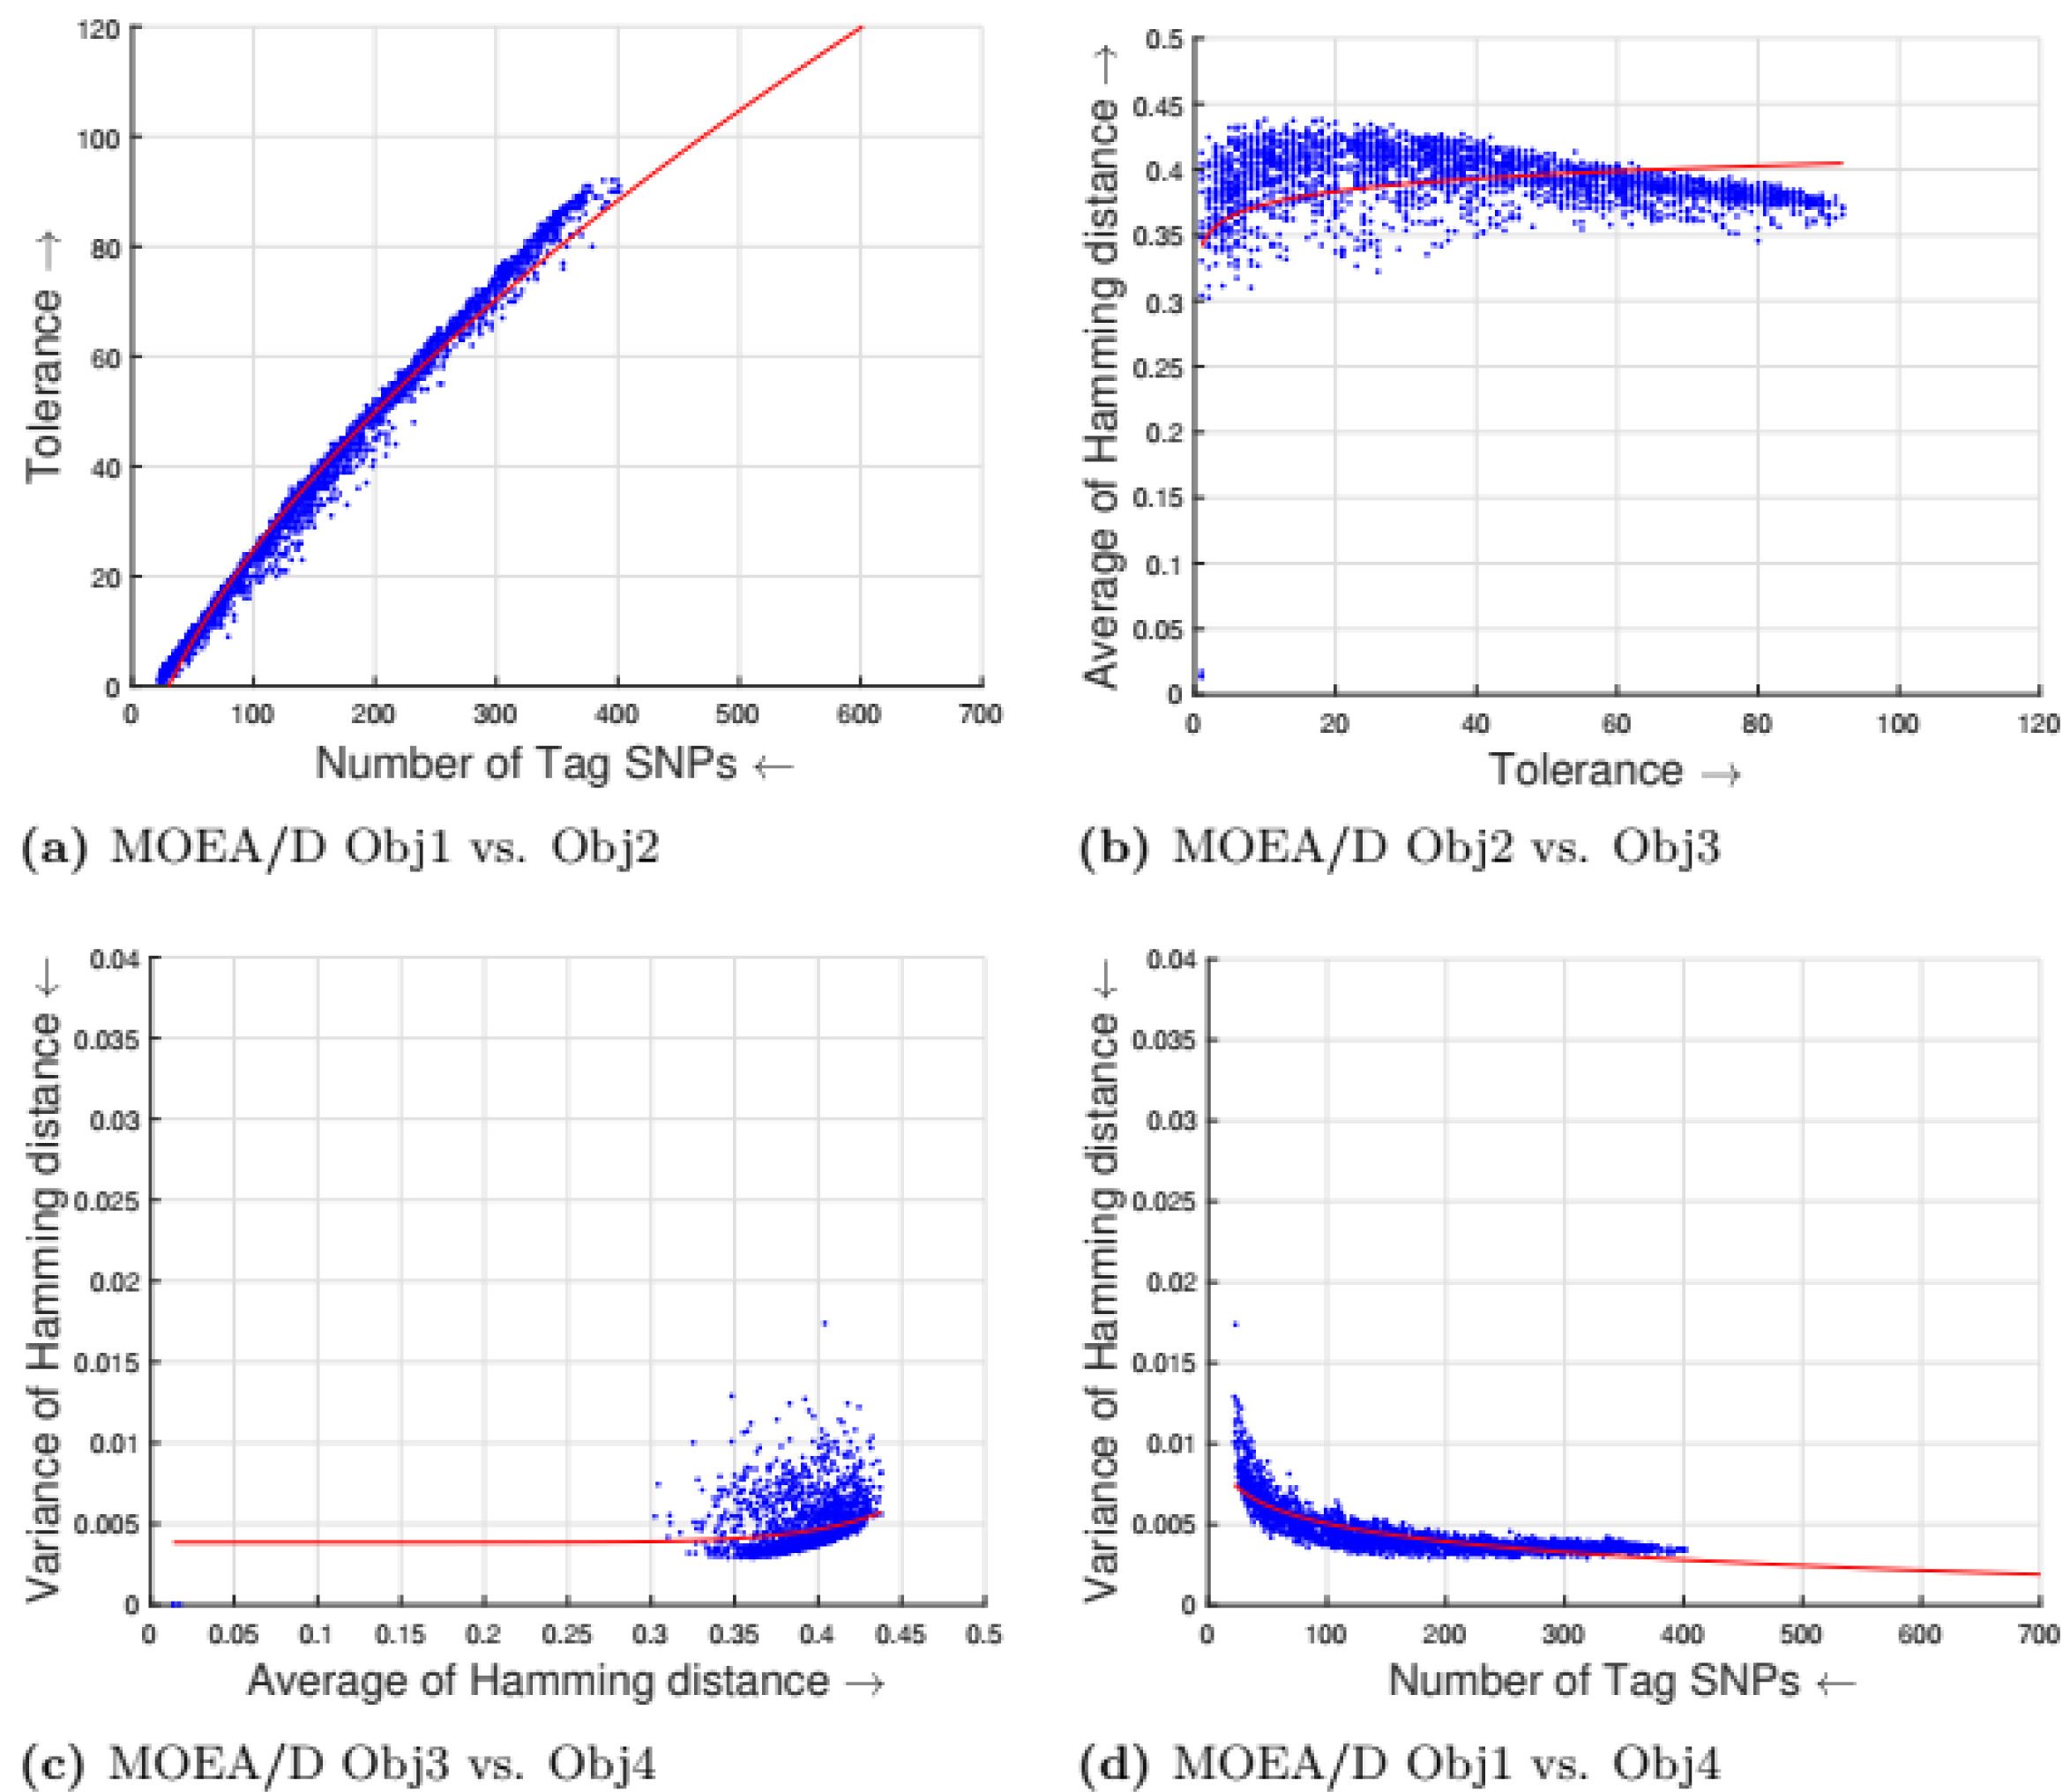
\includegraphics[width=0.18\textwidth]{analisis_assets/moqa_2022/figures/moqa_fig_moead_greedy.jpeg} &
        
\includegraphics[width=0.18\textwidth]{analisis_assets/20260430T185224/2_comparativa/1_frentes/frentes_pareto/frentes_pareto_moead_ws_greedy_ting_full.png} &
        
\includegraphics[width=0.18\textwidth]{analisis_assets/20260430T185224/2_comparativa/1_frentes/frentes_pareto/frentes_pareto_moead_ws_greedy_hybrid_full.png} &
        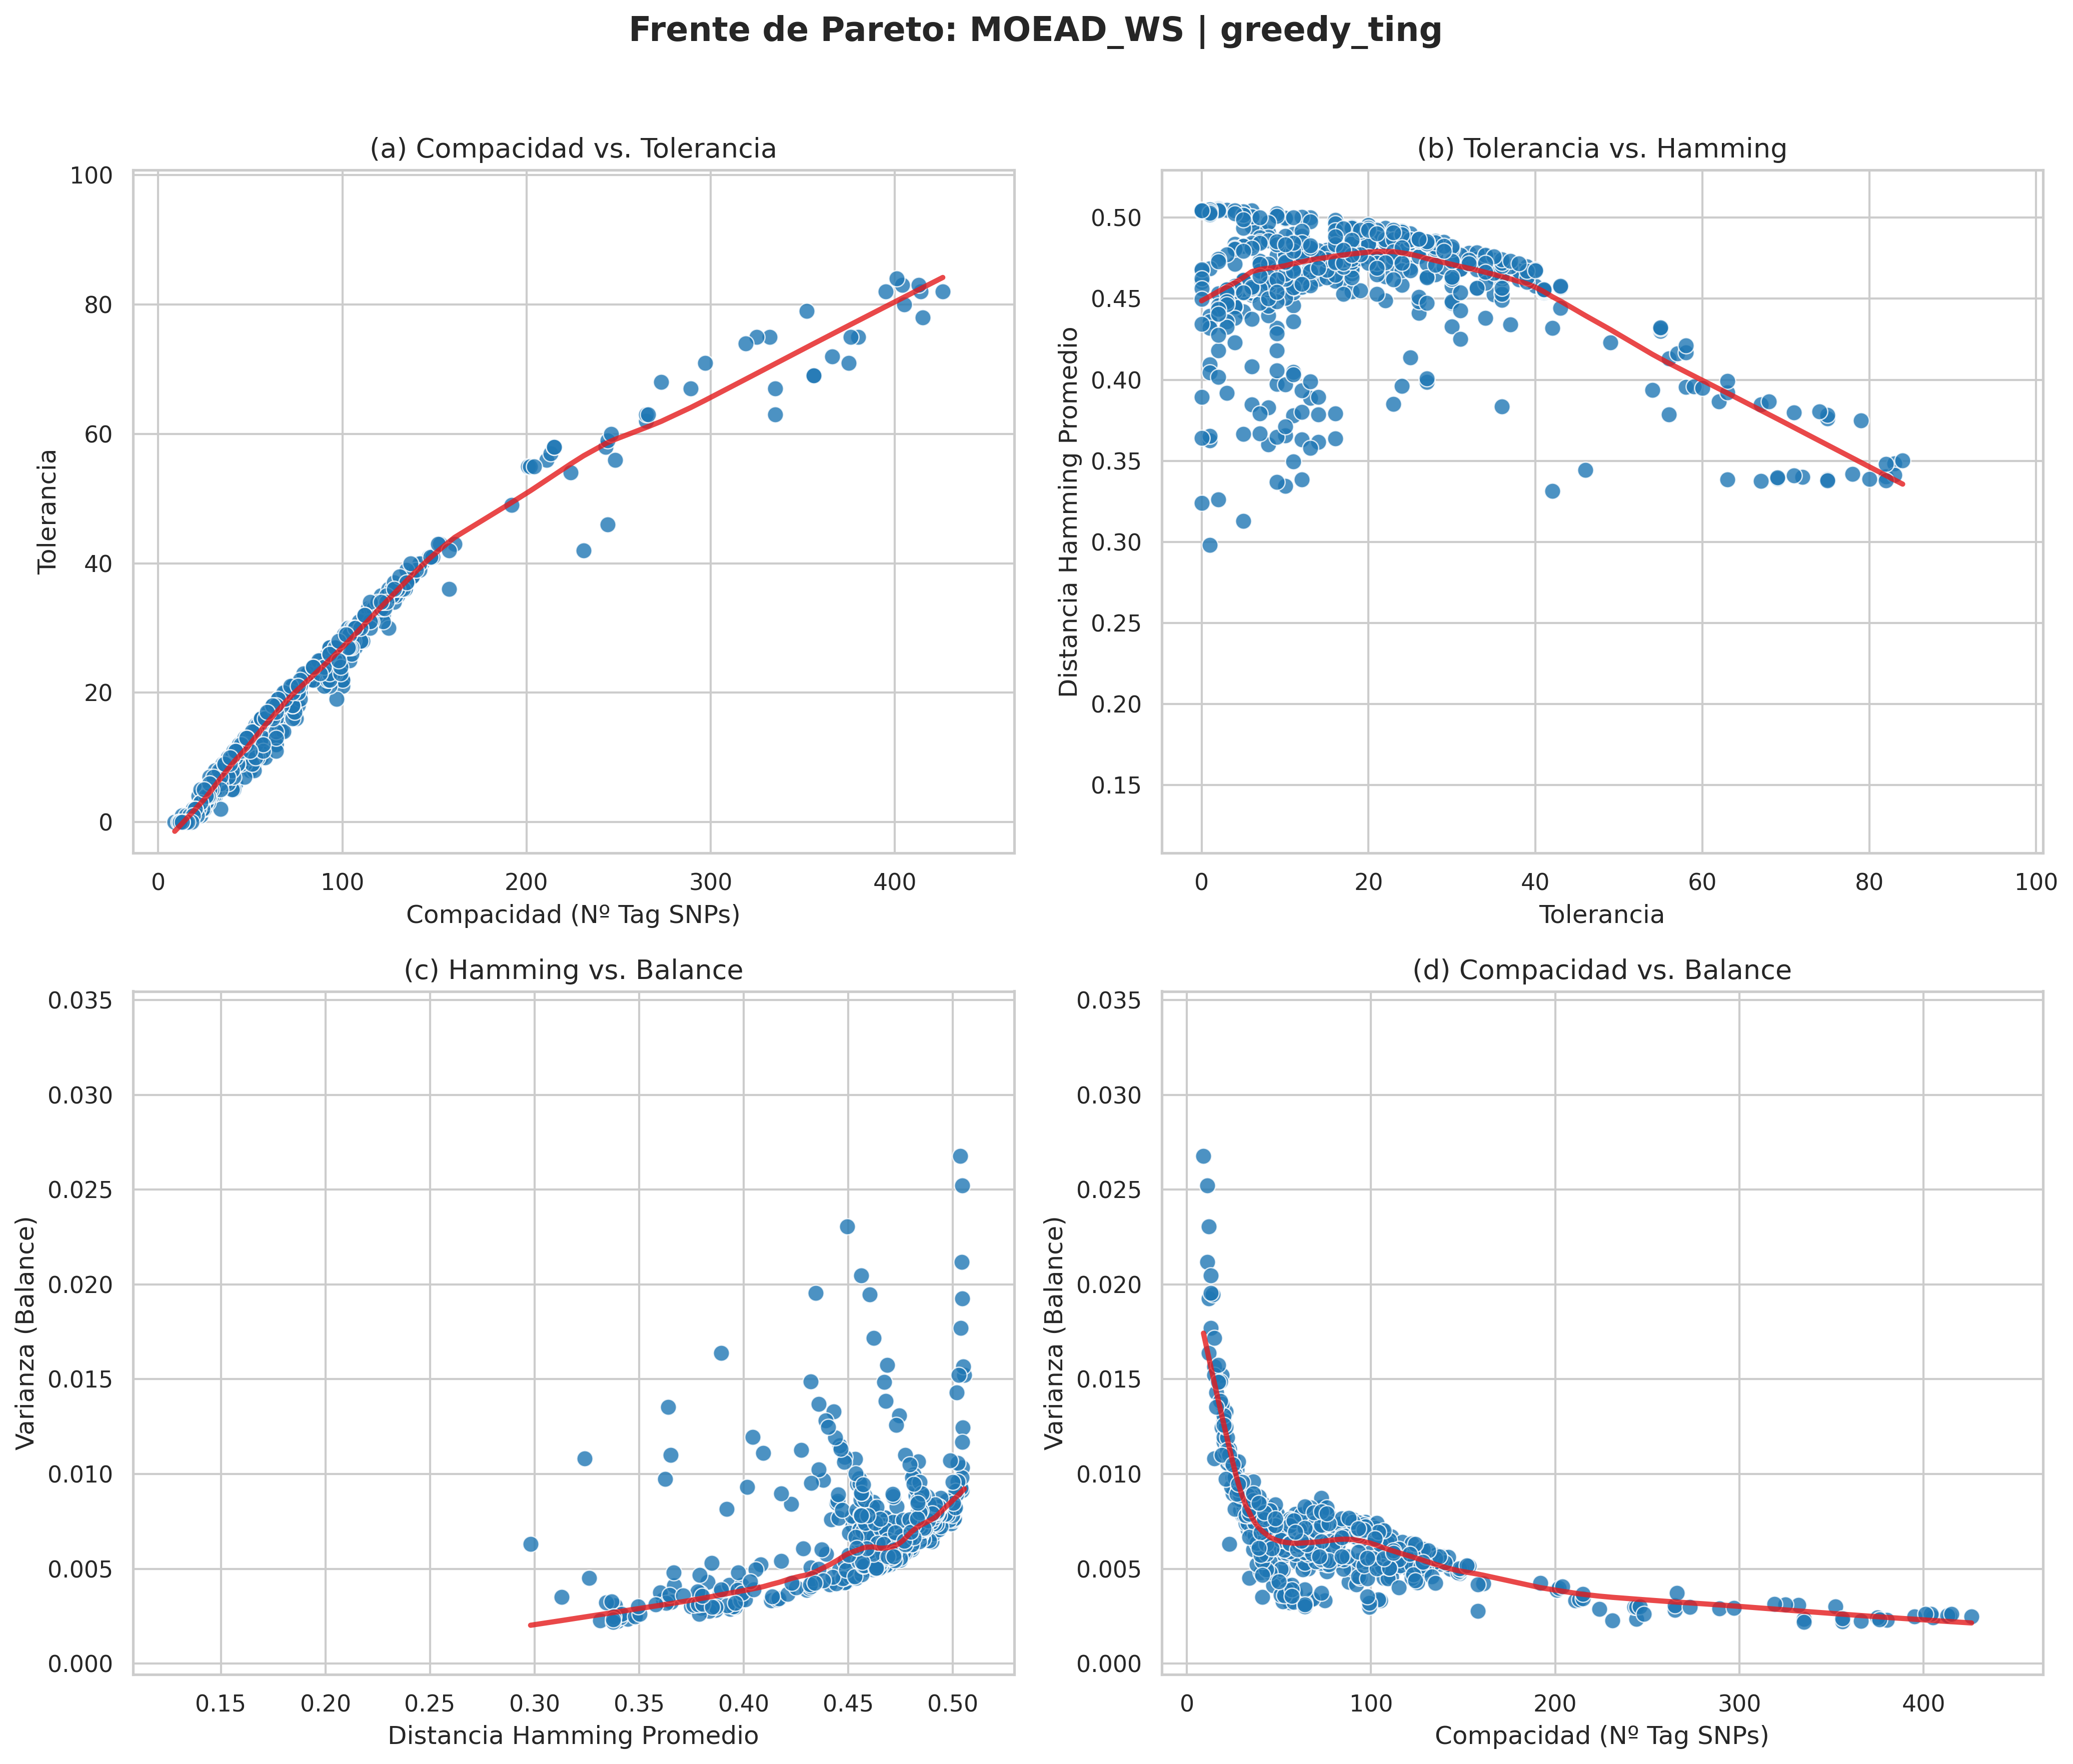
\includegraphics[width=0.18\textwidth]{analisis_assets/20260430T183144/2_comparativa/1_frentes/frentes_pareto/frentes_pareto_moead_ws_greedy_ting_full.png} &
        
\includegraphics[width=0.18\textwidth]{analisis_assets/20260430T183144/2_comparativa/1_frentes/frentes_pareto/frentes_pareto_moead_ws_greedy_hybrid_full.png} \\
        Moqa & Exp. A (GT) & Exp. A (GH) & Exp. B (GT) & Exp. B (GH) \\
    \end{tabular}
    \caption{Comparativa de frentes Greedy para MOEA/D-WS frente al original de Moqa.}
\end{figure}

\begin{itemize}
    \item \textbf{Similitudes:} Se observa una topología parecida en la proyección del frente (0,1).
    \item \textbf{Diferencias:} Se aprecian discrepancias en la proyección (1,1), donde las soluciones obtenidas tienden hacia el origen mientras que en Moqa están más repartidas. Además, los frentes (0,0) y (0,1) de A y B tienden a ser más extensos.
\end{itemize}

\begin{figure}[H]
    \centering
    \begin{tabular}{@{}ccc@{}}
        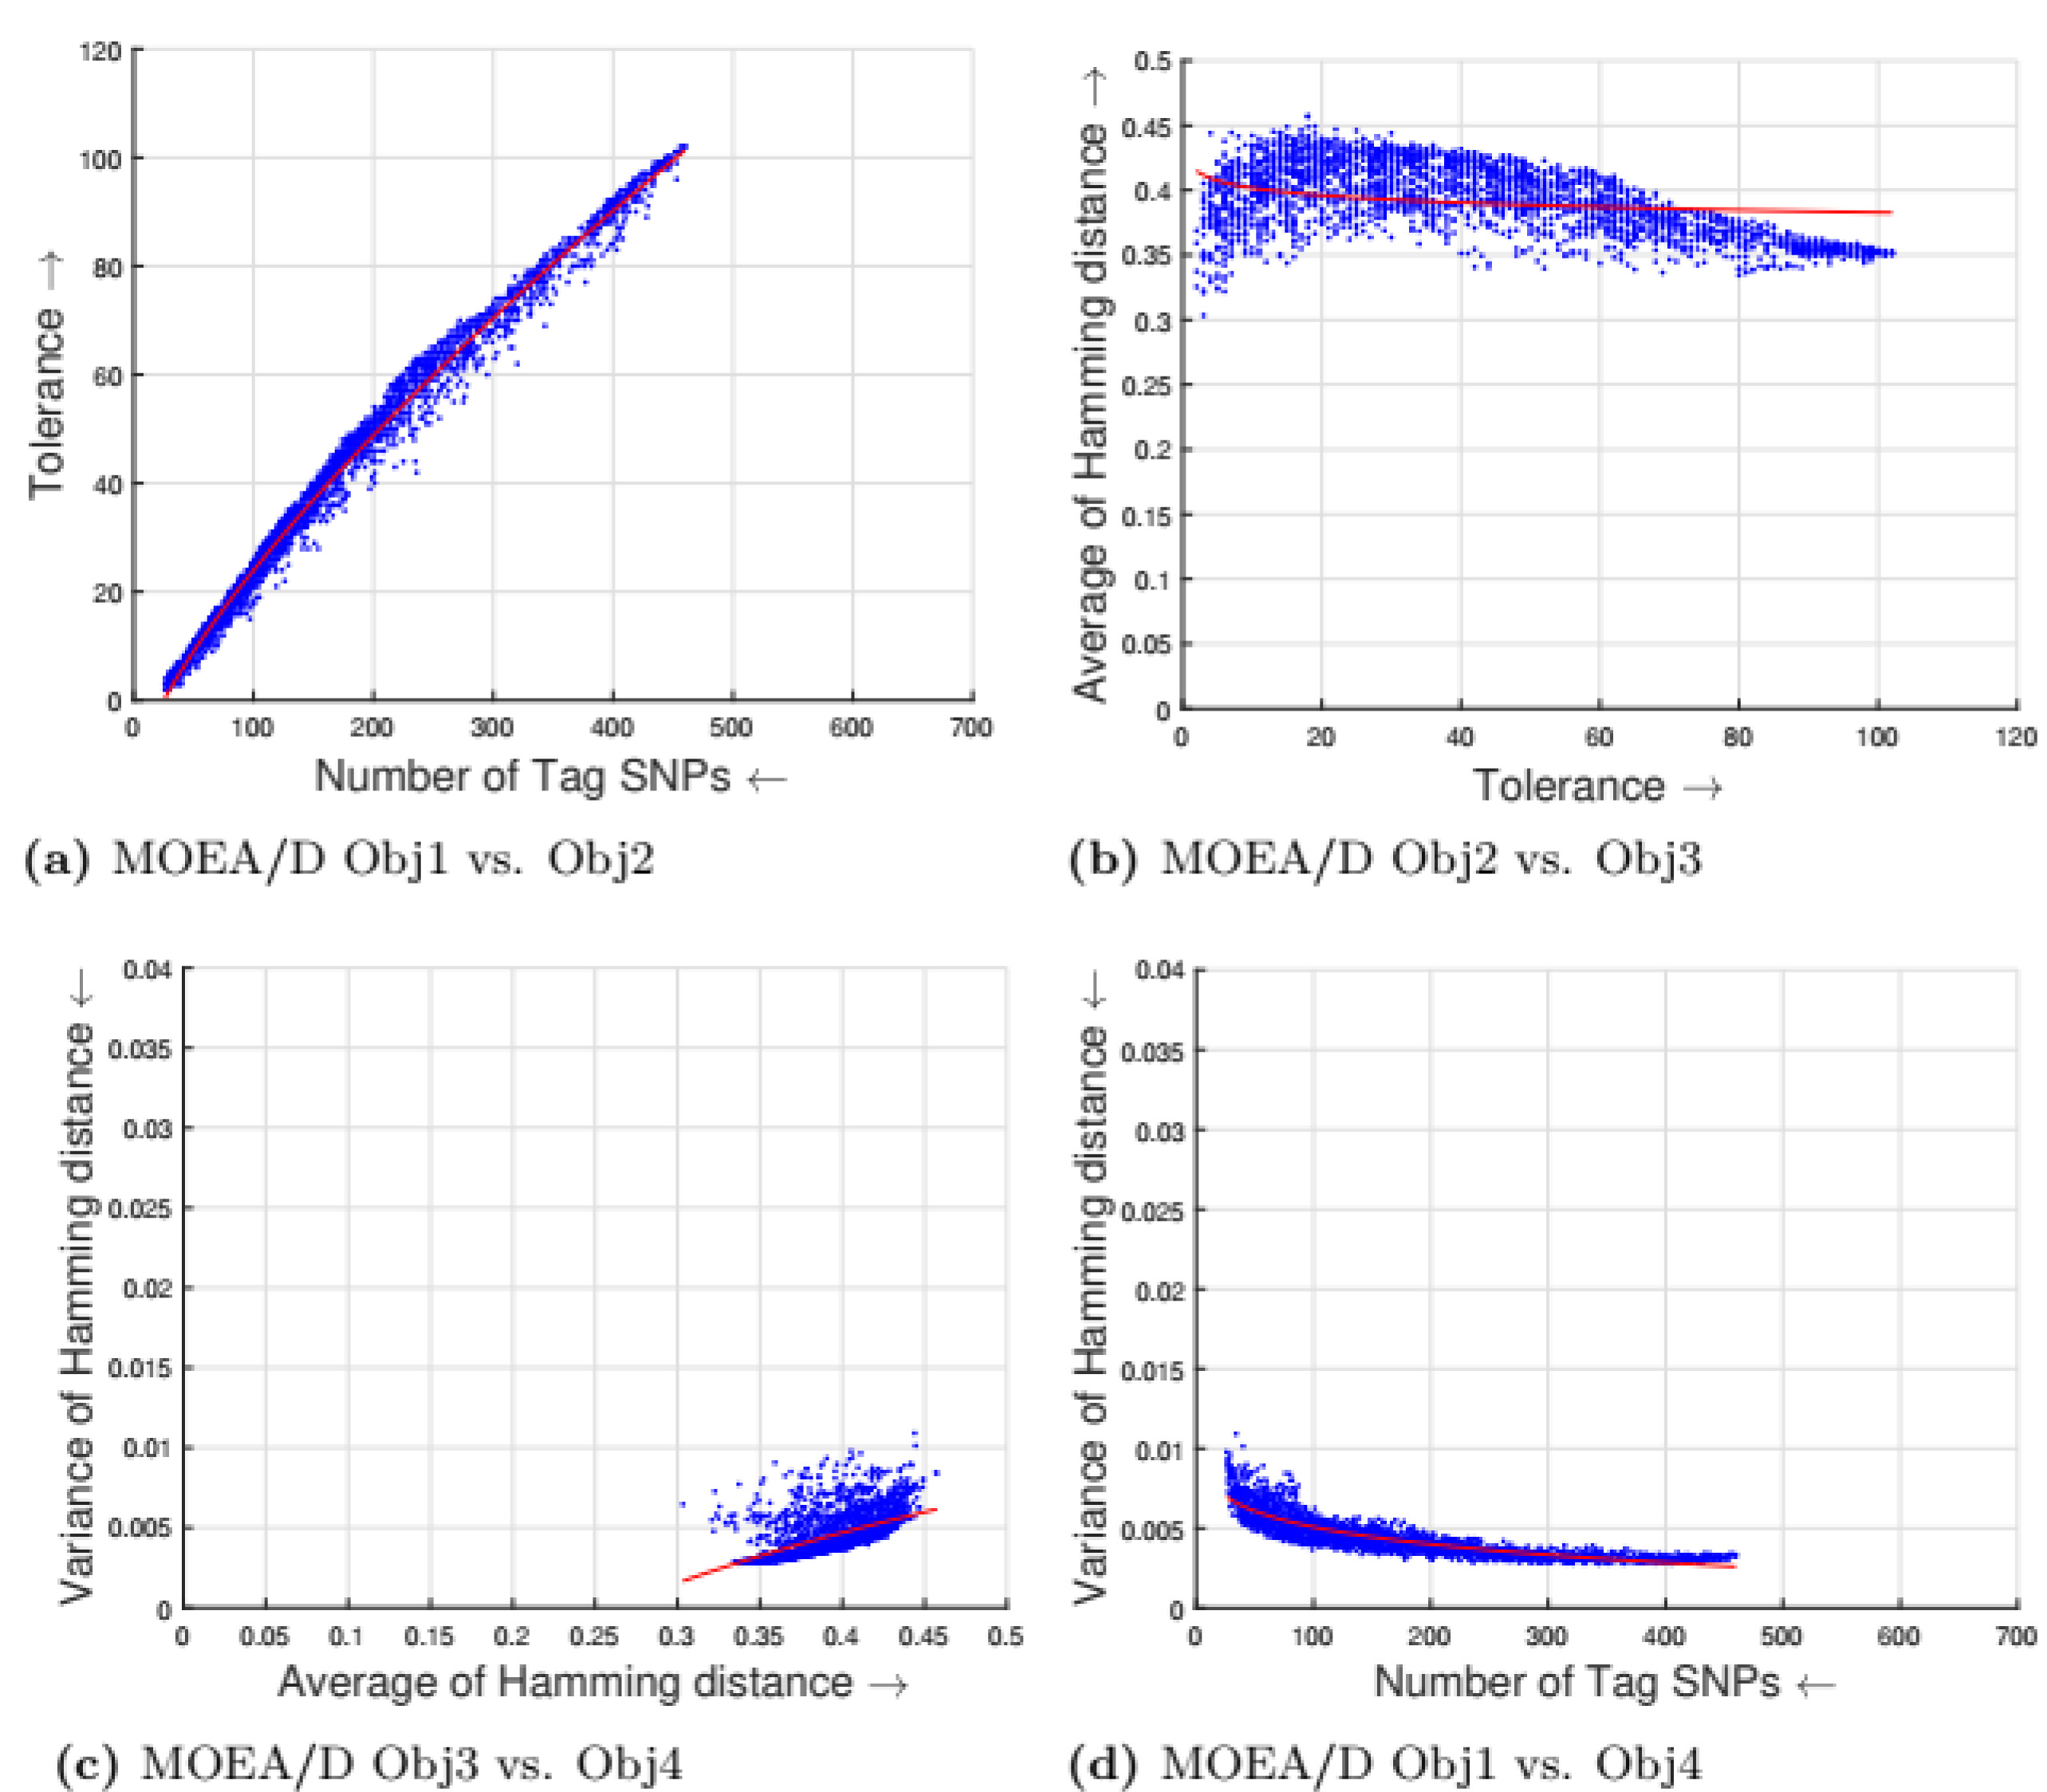
\includegraphics[width=0.28\textwidth]{analisis_assets/moqa_2022/figures/moqa_fig_moead_random.jpeg} &
        
\includegraphics[width=0.28\textwidth]{analisis_assets/20260430T185224/2_comparativa/1_frentes/frentes_pareto/frentes_pareto_moead_ws_random_dense_full.png} &
        
\includegraphics[width=0.28\textwidth]{analisis_assets/20260430T183144/2_comparativa/1_frentes/frentes_pareto/frentes_pareto_moead_ws_random_dense_full.png} \\
        Moqa & Exp. A (RD) & Exp. B (RD) \\
    \end{tabular}
    \caption{Comparativa de frentes Random para MOEA/D-WS frente al original de Moqa.}
\end{figure}

\begin{itemize}
    \item \textbf{Similitudes:} Se mantiene la consistencia en las líneas de tendencia suavizadas entre todos los experimentos comparados.
    \item \textbf{Diferencias:} Se observa que el frente reportado por Moqa alcanza una mayor extensión que los obtenidos en las simulaciones realizadas.
\end{itemize}
\subsection{Análisis Numérico y Estadístico por Métricas}
Tras la inspección visual, se procede al análisis de jerarquías de rendimiento. A continuación, se presenta el contraste de los rankings Top 8 para cada métrica, enfrentando los resultados originales de Moqa (2022) con las ejecuciones A y B de este TFG.

\subsubsection{Métrica 1: Range \texorpdfstring{($\uparrow$)}{(up)}}
\begin{table}[H]
    \centering
    \begin{minipage}[t]{0.32\textwidth}
        \centering\scriptsize\textbf{Moqa (2022)}\\
        \begin{tabular}{rl}
            \toprule
            Pos & Algo+Init \\ \midrule
            1 & MOEAD+R \\
            2 & MOEAD+G \\
            3 & NSGA2+G \\
            4 & NSGA2+R \\
            5 & NSGA3+G \\
            6 & SPEA2+R \\
            7 & SPEA2+G \\
            8 & NSGA3+R \\
            \bottomrule
        \end{tabular}
    \end{minipage}
    \hfill
    \begin{minipage}[t]{0.32\textwidth}
        \centering\scriptsize\textbf{Exp. A (neg)}\\
        \begin{tabular}{rl}
            \toprule
            Pos & Algo+Init \\ \midrule
            1 & NSGA2+GT \\
            2 & MOEAD\_W+GT \\
            3 & NSGA2+GH \\
            4 & MOEAD\_W+GH \\
            5 & MOEAD\_T+GT \\
            6 & NSGA3+GH \\
            7 & NSGA3+GT \\
            8 & MOEAD\_T+GH \\
            \bottomrule
        \end{tabular}
    \end{minipage}
    \hfill
    \begin{minipage}[t]{0.32\textwidth}
        \centering\scriptsize\textbf{Exp. B (inv)}\\
        \begin{tabular}{rl}
            \toprule
            Pos & Algo+Init \\ \midrule
            1 & NSGA2+GT \\
            2 & NSGA2+GH \\
            3 & SPEA2+GT \\
            4 & SPEA2+GH \\
            5 & NSGA2+RS \\
            6 & SPEA2+RS \\
            7 & MOEAD\_T+GH \\
            8 & MOEAD\_W+GH \\
            \\
            \bottomrule
        \end{tabular}
    \end{minipage}
    \caption{Comparativa de Rankings: Range (Extensión del frente).}
\end{table}

\textbf{Análisis comparativo entre experimentos:}
\begin{itemize}
    \item \textbf{Similitudes:} Además del claro dominio de las inicializaciones heurísticas (Greedy) en los tres entornos, destaca la consistencia estructural de NSGA-II. Este algoritmo logra posicionarse en el Top 4 de todos los ecosistemas experimentales (Moqa, A y B) para la maximización del rango, compartiendo el liderazgo en A y dominando por completo en B.
    \item \textbf{Discrepancias:} Mientras que en Moqa (2022) MOEA/D lidera el ranking en exclusiva, en las experimentaciones realizadas se observa una fuerte competencia con NSGA-II. Adicionalmente, las inicializaciones aleatorias de baja densidad (RS) adquieren relevancia significativa únicamente en el experimento B.
\end{itemize}


\subsubsection{Métrica 2: SumMin \texorpdfstring{($\downarrow$)}{(down)}}
\begin{table}[H]
    \centering
    \begin{minipage}[t]{0.32\textwidth}
        \centering\scriptsize\textbf{Moqa (2022)}\\
        \begin{tabular}{rl}
            \toprule
            Pos & Algo+Init \\ \midrule
            1 & MOEAD+G \\
            2 & NSGA3+G \\
            3 & MOEAD+R \\
            4 & NSGA2+G \\
            5 & NSGA2+R \\
            6 & SPEA2+G \\
            7 & SPEA2+R \\
            8 & NSGA3+R \\
            \\
            \bottomrule
        \end{tabular}
    \end{minipage}
    \hfill
    \begin{minipage}[t]{0.32\textwidth}
        \centering\scriptsize\textbf{Exp. A (neg)}\\
        \begin{tabular}{rl}
            \toprule
            Pos & Algo+Init \\ \midrule
            1 & NSGA2+GT \\
            2 & MOEAD\_W+GT \\
            3 & NSGA2+GH \\
            4 & MOEAD\_T+GT \\
            5 & NSGA3+GH \\
            6 & NSGA3+GT \\
            7 & MOEAD\_W+GH \\
            8 & MOEAD\_T+GH \\
            \\
            \bottomrule
        \end{tabular}
    \end{minipage}
    \hfill
    \begin{minipage}[t]{0.32\textwidth}
        \centering\scriptsize\textbf{Exp. B (inv)}\\
        \begin{tabular}{rl}
            \toprule
            Pos & Algo+Init \\ \midrule
            1 & NSGA2+GT \\
            2 & NSGA2+GH \\
            3 & MOEAD\_W+GH \\
            4 & MOEAD\_T+GH \\
            5 & SPEA2+GH \\
            6 & SPEA2+GT \\
            7 & MOEAD\_W+GT \\
            8 & NSGA2+RS \\
            \\
            \bottomrule
        \end{tabular}
    \end{minipage}
    \caption{Comparativa de Rankings: SumMin (Convergencia al ideal).}
\end{table}

\textbf{Análisis comparativo entre experimentos:}
\begin{itemize}
    \item \textbf{Similitudes:} El predominio de las estrategias basadas en heurísticas (Greedy) se observa transversalmente en los tres experimentos, consolidando su ventaja generalizada en esta métrica.
    \item \textbf{Discrepancias:} Moqa reporta a MOEA/D como la opción de mejor convergencia al ideal. Por el contrario, en los experimentos A y B de este trabajo, NSGA-II encabeza de forma consistente las jerarquías.
\end{itemize}


\subsubsection{Métrica 3: MinSum \texorpdfstring{($\downarrow$)}{(down)}}
\begin{table}[H]
    \centering
    \begin{minipage}[t]{0.32\textwidth}
        \centering\scriptsize\textbf{Moqa (2022)}\\
        \begin{tabular}{rl}
            \toprule
            Pos & Algo+Init \\ \midrule
            1 & MOEAD+G \\
            2 & MOEAD+R \\
            3 & NSGA2+G \\
            4 & NSGA2+R \\
            5 & SPEA2+G \\
            6 & SPEA2+R \\
            7 & NSGA3+G \\
            8 & NSGA3+R \\
            \\
            \bottomrule
        \end{tabular}
    \end{minipage}
    \hfill
    \begin{minipage}[t]{0.32\textwidth}
        \centering\scriptsize\textbf{Exp. A (neg)}\\
        \begin{tabular}{rl}
            \toprule
            Pos & Algo+Init \\ \midrule
            1 & NSGA3+RD \\
            2 & MOEAD\_T+GT \\
            3 & SPEA2+RD \\
            4 & MOEAD\_P+GT \\
            5 & MOEAD\_T+RD \\
            6 & MOEAD\_T+GH \\
            7 & MOEAD\_P+GH \\
            8 & NSGA2+RD \\
            \bottomrule
        \end{tabular}
    \end{minipage}
    \hfill
    \begin{minipage}[t]{0.32\textwidth}
        \centering\scriptsize\textbf{Exp. B (inv)}\\
        \begin{tabular}{rl}
            Pos & Algo+Init \\ \midrule
            1 & MOEAD\_W+GH \\
            2 & MOEAD\_W+GT \\
            3 & MOEAD\_T+GH \\
            4 & MOEAD\_T+GT \\
            5 & MOEAD\_T+RS \\
            6 & MOEAD\_W+RS \\
            7 & NSGA3+GH \\
            8 & NSGA3+GT \\
            \bottomrule
        \end{tabular}
    \end{minipage}
    \caption{Comparativa de Rankings: MinSum (Mejor solución individual).}
\end{table}

\textbf{Análisis comparativo entre experimentos:}
\begin{itemize}
    \item \textbf{Similitudes:} En el estudio original de Moqa y en el entorno recíproco (B), MOEA/D destaca de forma consistente en las primeras posiciones. La naturaleza escalarizadora de MOEA/D parece facilitar enormemente la convergencia hacia soluciones individuales extremas en la mayoría de escenarios evaluados.
    \item \textbf{Discrepancias:} Se observa una fuerte discrepancia en el entorno lineal (A). Mientras que Moqa y el experimento B consolidan a MOEA/D, en el entorno A las inicializaciones aleatorias densas (RD) adquieren un protagonismo inusual, catapultando a algoritmos como NSGA-III (1º posición) e incluso a SPEA2 (3º posición) por encima de varias configuraciones de MOEA/D. Este comportamiento sugiere que la topología del espacio lineal favorece estrategias de búsqueda basadas puramente en dominancia cuando la población inicial cubre suficientemente el espacio genómico.
\end{itemize}


\subsubsection{Métrica 4: MaxToleranceRate \texorpdfstring{($\uparrow$)}{(up)}}
\begin{table}[H]
    \centering
    \begin{minipage}[t]{0.32\textwidth}
        \centering\scriptsize\textbf{Moqa (2022)}\\
        \begin{tabular}{rl}
            \toprule
            Pos & Algo+Init \\ \midrule
            1 & NSGA3+G \\
            2 & NSGA3+R \\
            3 & MOEAD+R \\
            4 & MOEAD+G \\
            5 & NSGA2+G \\
            6 & NSGA2+R \\
            7 & SPEA2+G \\
            8 & SPEA2+R \\
            \\
            \bottomrule
        \end{tabular}
    \end{minipage}
    \hfill
    \begin{minipage}[t]{0.32\textwidth}
        \centering\scriptsize\textbf{Exp. A (neg)}\\
        \begin{tabular}{rl}
            \toprule
            Pos & Algo+Init \\ \midrule
            1 & MOEAD\_P+GT \\
            2 & MOEAD\_T+GT \\
            3 & MOEAD\_P+GH \\
            4 & NSGA3+RS \\
            5 & NSGA3+RD \\
            6 & MOEAD\_T+GH \\
            7 & SPEA2+RD \\
            8 & NSGA2+RD \\
            \\
            \bottomrule
        \end{tabular}
    \end{minipage}
    \hfill
    \begin{minipage}[t]{0.32\textwidth}
        \centering\scriptsize\textbf{Exp. B (inv)}\\
        \begin{tabular}{rl}
            \toprule
            Pos & Algo+Init \\ \midrule
            1 & MOEAD\_W+GT \\
            2 & MOEAD\_W+GH \\
            3 & MOEAD\_T+GT \\
            4 & NSGA3+RD \\
            5 & MOEAD\_T+GH \\
            6 & MOEAD\_T+RS \\
            7 & MOEAD\_W+RS \\
            8 & NSGA2+RD \\
            \\
            \bottomrule
        \end{tabular}
    \end{minipage}
    \caption{Comparativa de Rankings: Max Tolerance ($f_1$).}
\end{table}

\textbf{Análisis comparativo entre experimentos:}
\begin{itemize}
    \item \textbf{Similitudes:} Las implementaciones basadas en NSGA-III y MOEA/D son consistentemente competitivas a lo largo de los tres experimentos para buscar soluciones con picos de tolerancia.
    \item \textbf{Discrepancias:} En el artículo de Moqa, NSGA-III encabeza el ranking absoluto para la maximización de la tolerancia máxima. Sin embargo, en los experimentos de este trabajo (tanto A como B), son las distintas variantes de MOEA/D (PBI en A, WS en B) las que alcanzan sistemáticamente el primer puesto, desplazando a NSGA-III.
\end{itemize}


\subsubsection{Métrica 5: AvgToleranceRate \texorpdfstring{($\uparrow$)}{(up)}}
\begin{table}[H]
    \centering
    \begin{minipage}[t]{0.32\textwidth}
        \centering\scriptsize\textbf{Moqa (2022)}\\
        \begin{tabular}{rl}
            \toprule
            Pos & Algo+Init \\ \midrule
            1 & MOEAD+R \\
            2 & MOEAD+G \\
            3 & NSGA3+R \\
            4 & NSGA3+G \\
            5 & NSGA2+G \\
            6 & NSGA2+R \\
            7 & SPEA2+G \\
            8 & SPEA2+R \\
            \\
            \bottomrule
        \end{tabular}
    \end{minipage}
    \hfill
    \begin{minipage}[t]{0.32\textwidth}
        \centering\scriptsize\textbf{Exp. A (neg)}\\
        \begin{tabular}{rl}
            \toprule
            Pos & Algo+Init \\ \midrule
            1 & NSGA3+RD \\
            2 & MOEAD\_P+GT \\
            3 & MOEAD\_P+GH \\
            4 & MOEAD\_T+RD \\
            5 & SPEA2+RD \\
            6 & MOEAD\_W+RD \\
            7 & MOEAD\_P+RS \\
            8 & NSGA2+RD \\
            \\
            \bottomrule
        \end{tabular}
    \end{minipage}
    \hfill
    \begin{minipage}[t]{0.32\textwidth}
        \centering\scriptsize\textbf{Exp. B (inv)}\\
        \begin{tabular}{rl}
            \toprule
            Pos & Algo+Init \\ \midrule
            1 & NSGA3+RD \\
            2 & MOEAD\_W+GT \\
            3 & NSGA2+RD \\
            4 & MOEAD\_W+GH \\
            5 & MOEAD\_W+RS \\
            6 & MOEAD\_P+RS \\
            7 & MOEAD\_W+RD \\
            8 & MOEAD\_T+GT \\
            \\
            \bottomrule
        \end{tabular}
    \end{minipage}
    \caption{Comparativa de Rankings: Avg Tolerance.}
\end{table}

\textbf{Análisis comparativo entre experimentos:}
\begin{itemize}
    \item \textbf{Similitudes:} NSGA-III y MOEA/D se consolidan como los algoritmos con mayor capacidad para mantener una elevada tolerancia media en la población.
    \item \textbf{Discrepancias:} Moqa reporta a MOEA/D como líder indiscutible para la métrica media. Contrastando con ello, en las ejecuciones A y B de este trabajo es NSGA-III con inicialización densa (RD) quien encabeza la tabla. La ventaja de las semillas densas para preservar valores altos medios biológicos es una dinámica no contemplada en el estudio original.
\end{itemize}


\subsubsection{Métrica 6: Avg Hamming Distance (\texorpdfstring{$f_3$}{f3}) \texorpdfstring{($\uparrow$)}{(up)}}
\begin{table}[H]
    \centering
    \begin{minipage}[t]{0.32\textwidth}
        \centering\scriptsize\textbf{Moqa (2022)}\\
        \begin{tabular}{rl}
            \toprule
            Pos & Algo+Init \\ \midrule
            1 & SPEA2+G \\
            2 & SPEA2+R \\
            3 & NSGA2+R \\
            4 & NSGA2+G \\
            5 & NSGA3+G \\
            6 & NSGA3+R \\
            7 & MOEAD+G \\
            8 & MOEAD+R \\
            \\
            \bottomrule
        \end{tabular}
    \end{minipage}
    \hfill
    \begin{minipage}[t]{0.32\textwidth}
        \centering\scriptsize\textbf{Exp. A (neg)}\\
        \begin{tabular}{rl}
            \toprule
            Pos & Algo+Init \\ \midrule
            1 & MOEAD\_W+GH \\
            2 & MOEAD\_W+RS \\
            3 & MOEAD\_W+GT \\
            4 & MOEAD\_T+RS \\
            5 & MOEAD\_T+GH \\
            6 & MOEAD\_T+GT \\
            7 & NSGA3+RS \\
            8 & MOEAD\_P+RS \\
            \\
            \bottomrule
        \end{tabular}
    \end{minipage}
    \hfill
    \begin{minipage}[t]{0.32\textwidth}
        \centering\scriptsize\textbf{Exp. B (inv)}\\
        \begin{tabular}{rl}
            \toprule
            Pos & Algo+Init \\ \midrule
            1 & MOEAD\_W+GH \\
            2 & MOEAD\_W+GT \\
            3 & MOEAD\_T+GH \\
            4 & MOEAD\_T+RS \\
            5 & MOEAD\_T+GT \\
            6 & MOEAD\_W+RS \\
            7 & MOEAD\_P+RS \\
            8 & MOEAD\_P+GH \\
            \\
            \bottomrule
        \end{tabular}
    \end{minipage}
    \caption{Comparativa de Rankings: Diversidad de Hamming ($f_3$).}
\end{table}

\textbf{Análisis comparativo entre experimentos:}
\begin{itemize}
    \item \textbf{Similitudes:} Tan solo la superioridad de MOEA/D en las posiciones más altas de los experimentos A y B.
    \item \textbf{Discrepancias:} Moqa reporta un liderazgo contundente de SPEA2 para preservar la diversidad. Por el contrario, en los experimentos A y B, MOEA/D (en particular la variante WS) domina ampliamente esta métrica. Esta disparidad tan aguda evidencia que las dinámicas de preservación de diversidad divergen radicalmente dependiendo de los detalles de implementación subyacentes.
\end{itemize}


\subsubsection{Métrica 7: Hypervolume \texorpdfstring{($\uparrow$)}{(up)}}
\begin{table}[H]
    \centering
    \begin{minipage}[t]{0.32\textwidth}
        \centering\scriptsize\textbf{Moqa (2022)}\\
        \begin{tabular}{rl}
            \toprule
            Pos & Algo+Init \\ \midrule
            1 & Sin datos \\
            2 & Sin datos \\
            3 & Sin datos \\
            4 & Sin datos \\
            5 & Sin datos \\
            6 & Sin datos \\
            7 & Sin datos \\
            8 & Sin datos \\
            \bottomrule
        \end{tabular}
    \end{minipage}
    \hfill
    \begin{minipage}[t]{0.32\textwidth}
        \centering\scriptsize\textbf{Exp. A (neg)}\\
        \begin{tabular}{rl}
            \toprule
            Pos & Algo+Init \\ \midrule
            1 & MOEAD\_T+GT \\
            2 & NSGA2+RD \\
            3 & MOEAD\_T+GH \\
            4 & NSGA3+GT \\
            5 & NSGA2+GT \\
            6 & NSGA3+GH \\
            7 & NSGA3+RD \\
            8 & MOEAD\_P+GT \\
            \bottomrule
        \end{tabular}
    \end{minipage}
    \hfill
    \begin{minipage}[t]{0.32\textwidth}
        \centering\scriptsize\textbf{Exp. B (inv)}\\
        \begin{tabular}{rl}
            \toprule
            Pos & Algo+Init \\ \midrule
            1 & MOEAD\_W+GH \\
            2 & MOEAD\_W+GT \\
            3 & MOEAD\_T+GH \\
            4 & NSGA3+GT \\
            5 & NSGA3+GH \\
            6 & NSGA2+GH \\
            7 & MOEAD\_T+GT \\
            8 & NSGA2+GT \\
            \bottomrule
        \end{tabular}
    \end{minipage}
    \caption{Comparativa de Rankings: Hypervolume global.}
\end{table}

\textbf{Análisis comparativo entre experimentos:}
\begin{itemize}
    \item \textbf{Similitudes:} (Comparación limitada a A y B) En ambos ecosistemas experimentales, las arquitecturas MOEA/D combinadas con esquemas de inicialización Greedy (GT y GH) dominan las primeras posiciones, demostrando gran eficiencia en la cobertura espacial.
    \item \textbf{Discrepancias:} La principal discrepancia reside en la ausencia de esta métrica en los resultados tabulados de Moqa et al. (2022). En las evaluaciones desarrolladas en este estudio, el entorno lineal (A) permite a algoritmos clásicos como NSGA-II emerger en posiciones altas (Top 2), mientras que en el espacio recíproco (B), MOEA/D acapara de forma más restrictiva el liderazgo.
\end{itemize}

\subsection{Análisis del Ranking Global (Average Rank)}

Tras evaluar cada métrica de forma individual, se procede al análisis del \textit{Average Rank} global, el cual sintetiza el desempeño de cada configuración a través de las dimensiones del estudio. Este análisis se divide en dos enfoques: uno integrado que incluye todas las métricas del TFG, y otro de comparabilidad que omite el \textit{Hypervolume} para alinearse con las métricas disponibles en el estudio original.

\subsubsection{Ranking Global Integrado (7 métricas) \texorpdfstring{($\downarrow$)}{(down)}}

Esta subsección presenta el ranking global considerando la totalidad de los indicadores calculados en este TFG, incluyendo el \textit{Hypervolume} como métrica fundamental de la calidad del frente.

Cabe destacar que esta comparativa no es complemente justa, ya que el estudio original no tiene en cuenta el hypervolume como métrica de evaluación de los algoritmos. Por ello, más adelante se realizará un análisis comparativo sin incluir el hypervolume. Aún así, el hypervolume es una métrica fundamental de la calidad del frente, por lo que se incluye en el análisis global.

\begin{table}[H]
    \centering
    \begin{minipage}[t]{0.32\textwidth}
        \centering\scriptsize\textbf{Moqa (2022)}\\
        \begin{tabular}{rl}
            \toprule
            Pos & Algo+Init \\ \midrule
            1 & MOEAD+G \\
            2 & MOEAD+R \\
            3 & NSGA3+G \\
            4 & NSGA2+G \\
            5 & NSGA2+R \\
            6 & SPEA2+G \\
            7 & NSGA3+R \\
            8 & SPEA2+R \\
            \bottomrule
        \end{tabular}
    \end{minipage}
    \hfill
    \begin{minipage}[t]{0.32\textwidth}
        \centering\scriptsize\textbf{Exp. A (neg)}\\
        \begin{tabular}{rl}
            \toprule
            Pos & Algo+Init \\ \midrule
            1 & MOEAD\_T+GH \\
            2 & MOEAD\_P+GH \\
            3 & NSGA3+RD \\
            4 & NSGA2+RD \\
            5 & SPEA2+RD \\
            6 & NSGA3+GH \\
            7 & NSGA2+GH \\
            8 & MOEAD\_T+RD \\
            \bottomrule
        \end{tabular}
    \end{minipage}
    \hfill
    \begin{minipage}[t]{0.32\textwidth}
        \centering\scriptsize\textbf{Exp. B (inv)}\\
        \begin{tabular}{rl}
            \toprule
            Pos & Algo+Init \\ \midrule
            1 & MOEAD\_W+GH \\
            2 & MOEAD\_T+GH \\
            3 & MOEAD\_T+RS \\
            4 & NSGA3+GH \\
            5 & MOEAD\_W+RS \\
            6 & NSGA2+GH \\
            7 & SPEA2+GH \\
            8 & MOEAD\_P+RS \\
            \bottomrule
        \end{tabular}
    \end{minipage}
    \caption{Comparativa de Rankings Globales Integrados (7 métricas).}
\end{table}

\textbf{Análisis comparativo (Ranking Integrado):}
\begin{itemize}
    \item \textbf{Similitudes:} El ranking integrado consolida a los algoritmos basados en descomposición (MOEA/D) como los más equilibrados. En todos los casos, variantes de MOEA/D bajo inicialización dirigida (G/GH) ocupan la primera posición, demostrando robustez al promediar rendimiento en convergencia, diversidad y volumen.
    \item \textbf{Discrepancias:} No se aprecian diferencias significativas. Aunque se hayan observado otras discrepancias en los rankings de métricas individuales, cuando se aplica un enfoque integrador, los resultados convergen hacia los mismos algoritmos, si bien sí se aprecian diferencias en cuanto a las incializaciones destacadas.
\end{itemize}

\subsubsection{Ranking Global de Comparabilidad (Sin Hypervolume) \texorpdfstring{($\downarrow$)}{(down)}}

Dado que el estudio original de Moqa et al. (2022) no reporta valores de \textit{Hypervolume}, esta subsección recalcula los rankings de los experimentos A y B omitiendo dicha métrica. Esto permite establecer una comparativa estrictamente basada en las 6 dimensiones compartidas: \textit{Range, SumMin, MinSum, MaxTolerance, AvgTolerance} y \textit{Hamming}.

\begin{table}[H]
    \centering
    \begin{minipage}[t]{0.32\textwidth}
        \centering\scriptsize\textbf{Moqa (2022)}\\
        \begin{tabular}{rl}
            \toprule
            Pos & Algo+Init \\ \midrule
            1 & MOEAD+G \\
            2 & MOEAD+R \\
            3 & NSGA3+G \\
            4 & NSGA2+G \\
            5 & NSGA2+R \\
            6 & SPEA2+G \\
            7 & NSGA3+R \\
            8 & SPEA2+R \\
            \bottomrule
        \end{tabular}
    \end{minipage}
    \hfill
    \begin{minipage}[t]{0.32\textwidth}
        \centering\scriptsize\textbf{Exp. A (neg)}\\
        \begin{tabular}{rl}
            \toprule
            Pos & Algo+Init \\ \midrule
            1 & MOEAD\_T+GH \\
            2 & MOEAD\_P+GH \\
            3 & NSGA3+RD \\
            4 & SPEA2+RD \\
            5 & NSGA2+RD \\
            6 & NSGA3+GH \\
            7 & MOEAD\_W+GH \\
            8 & MOEAD\_T+RD \\
            \bottomrule
        \end{tabular}
    \end{minipage}
    \hfill
    \begin{minipage}[t]{0.32\textwidth}
        \centering\scriptsize\textbf{Exp. B (inv)}\\
        \begin{tabular}{rl}
            \toprule
            Pos & Algo+Init \\ \midrule
            1 & MOEAD\_W+GH \\
            2 & MOEAD\_T+GH \\
            3 & MOEAD\_T+RS \\
            4 & NSGA3+GH \\
            5 & MOEAD\_W+RS \\
            6 & MOEAD\_P+RS \\
            7 & SPEA2+GH \\
            8 & NSGA2+GH \\
            \bottomrule
        \end{tabular}
    \end{minipage}
    \caption{Comparativa de Rankings Globales de Comparabilidad (6 métricas compartidas).}
\end{table}

\textbf{Análisis comparativo (Ranking sin Hypervolume):}
\begin{itemize}
    \item \textbf{Similitudes:} La estabilidad del ranking es el hallazgo más significativo. A pesar de retirar el indicador de volumen, el orden jerárquico de las 5 mejores configuraciones se mantiene prácticamente inalterado en ambos experimentos. Esto ratifica que el liderazgo de las variantes de MOEA/D (Tchebycheff en A y WeightSum en B) es estructural y responde a una superioridad consistente en la aproximación biológica y la convergencia de rangos, no a un sesgo de una métrica específica.
    \item \textbf{Discrepancias:} Las variaciones son mínimas y se limitan a ligeros ajustes en la mitad inferior del Top 8. En la Ejecución A, solo ocurre un intercambio de posiciones entre NSGA-II y SPEA-2 (puestos 4 y 5), mientras que en la B, la configuración \texttt{MOEAD\_P+RS} escala dos posiciones al no ser penalizada por su volumen. La alta correlación entre ambos rankings valida la robustez de la metodología y la fiabilidad de la comparativa con el paper original.
\end{itemize}

\subsection{Discusión General y Síntesis de Resultados}

Tras el análisis detallado de cada métrica y el estudio de los rankings globales, se presenta una síntesis integral que evalúe la solidez de los experimentos realizados frente al estado del arte:

\begin{itemize}
    \item \textbf{Compromiso entre Extensión y Densidad:} Mientras que el enfoque de Moqa (2022) tiende a generar frentes más densos y focalizados, lo que proporciona una gran granularidad de soluciones intermedias, las heurísticas desarrolladas en las ejecuciones A y B logran una mayor amplitud espacial (spread). Esto indica que las inicializaciones implementadas favorecen el descubrimiento de configuraciones extremas de Tag SNPs, ampliando el rango de opciones disponibles, aunque sacrificando en cierta medida la densidad y uniformidad del conjunto final de soluciones.
    \item \textbf{Limitaciones en la Replicabilidad:} Las diferencias morfológicas encontradas en los frentes de Pareto pueden señalar discrepancias no detalladas en las estrategias de inicialización y/o en la configuración interna de ciertos algoritmos. Sin disponer de esta información específica, resulta prácticamente imposible replicar el estudio original con total exactitud.
    \item \textbf{Consistencia Estructural con Moqa (2022):} A pesar de las discrepancias puntuales en el comportamiento de métricas individuales (especialmente bajo la transformación lineal de la Ejecución A), la tendencia macroscópica y la jerarquía de rendimiento de los algoritmos son consistentemente similares a las reportadas en el estudio original.
    \item \textbf{Superioridad de la Descomposición:} En las tres fuentes evaluadas (Moqa, Ejecución A y Ejecución B), MOEA/D emerge como el motor de optimización más equilibrado. Esto demuestra que la segmentación del problema en subproblemas escalares es la estrategia más robusta para el diseño de paneles de Tag SNPs, independientemente de la normalización o transformación de los objetivos aplicada.
    \item \textbf{Primacía de la Inicialización Heurística:} Se valida externamente que la calidad de la población inicial es el factor más determinante del éxito evolutivo. La brecha de rendimiento entre las configuraciones heurísticas (\texttt{greedy} / \texttt{greedy\_hybrid} / \texttt{greedy\_ting}) y las aleatorias es significativamente mayor que la diferencia entre los algoritmos evolutivos, tal como sugería el paper de referencia.
\end{itemize}
\section{Observaciones}
\label{sec:observaciones}

Durante el desarrollo de evaluaciones experimentales extendidas (como la serie \texttt{full\_20}, con 20 ejecuciones independientes por configuración sobre el conjunto Hinds2005), se ha observado un comportamiento estadístico que invita a la reflexión sobre el rendimiento real de los algoritmos.

Al someter los resultados a pruebas no paramétricas de rangos, concretamente el test de Friedman, se obtuvieron p-valores superiores al umbral de significancia ($p > 0,05$). Esto ocurre a pesar de que, en un análisis visual de las medias, ciertos algoritmos como MOEA/D aparentan una ligera ventaja. Por ejemplo, en métricas como el Hipervolumen, MOEA/D alcanzó promedios en torno a $1,2426 \pm 0,0171$, frente al $1,2422 \pm 0,0087$ de NSGA-III.

La diferencia entre ambas medias es del orden de $0,0004$, una magnitud sustancialmente menor que la desviación típica de las propias ejecuciones. Que el test de Friedman no detecte significancia estadística con 20 repeticiones sugiere la posibilidad de que, en realidad, no existan diferencias estructurales contundentes entre NSGA-II, NSGA-III y MOEA/D bajo estas configuraciones.

Es plausible que el aparente dominio de un método en las tablas de promedios se deba principalmente a la estocasticidad intrínseca de los operadores evolutivos y la influencia de la semilla inicial. Se sugiere, por tanto, interpretar los liderazgos algorítmicos con cautela, abriendo la puerta a la hipótesis de que diversos enfoques del estado del arte puedan ofrecer un rendimiento empíricamente equivalente para la selección de Tag SNPs.

\subsection{Resultados del Experimento \texttt{full\_20}}

A continuación se adjuntan los resultados numéricos (Top 8) y el resumen de la salida por terminal del experimento de validación estadística:

\begin{verbatim}
TOP 8 por Metrica (Resumen de Medias +/- Std)
------------------------------------------------
* Range (+)
     1. NSGA2 (greedy_ting): 2.2024 +/- 0.0620
     2. SPEA2 (greedy_ting): 1.8085 +/- 0.0621
     3. NSGA3 (greedy_ting): 1.5925 +/- 0.1190
     4. MOEAD_TCHE (greedy_ting): 1.4399 +/- 0.3870
     5. NSGA2 (random_dense): 0.5561 +/- 0.0303
     6. SPEA2 (random_dense): 0.4636 +/- 0.0665
     7. NSGA3 (random_dense): 0.3059 +/- 0.0210
     8. MOEAD_TCHE (random_dense): 0.2363 +/- 0.0365
* SumMin (-)
     1. NSGA2 (greedy_ting): 0.1250 +/- 0.0009
     2. MOEAD_TCHE (greedy_ting): 0.1541 +/- 0.0178
     3. NSGA3 (greedy_ting): 0.1564 +/- 0.0096
     4. SPEA2 (greedy_ting): 0.1632 +/- 0.0125
     5. SPEA2 (random_dense): 0.2910 +/- 0.0257
     6. NSGA2 (random_dense): 0.3328 +/- 0.0244
     7. NSGA3 (random_dense): 0.3738 +/- 0.0177
     8. MOEAD_TCHE (random_dense): 0.4739 +/- 0.0254
* MinSum (-)
     1. MOEAD_TCHE (greedy_ting): 0.2859 +/- 0.0095
     2. NSGA3 (greedy_ting): 0.2931 +/- 0.0078
     3. SPEA2 (greedy_ting): 0.3493 +/- 0.0112
     4. SPEA2 (random_dense): 0.3514 +/- 0.0171
     5. NSGA2 (greedy_ting): 0.3534 +/- 0.0153
     6. NSGA3 (random_dense): 0.3981 +/- 0.0152
     7. NSGA2 (random_dense): 0.4088 +/- 0.0459
     8. MOEAD_TCHE (random_dense): 0.5057 +/- 0.0238
* MaxToleranceRate (+)
     1. MOEAD_TCHE (greedy_ting): 0.2715 +/- 0.0066
     2. NSGA3 (random_dense): 0.2679 +/- 0.0037
     3. NSGA2 (random_dense): 0.2488 +/- 0.0069
     4. SPEA2 (random_dense): 0.2463 +/- 0.0082
     5. NSGA3 (greedy_ting): 0.2289 +/- 0.0129
     6. MOEAD_TCHE (random_dense): 0.2211 +/- 0.0057
     7. NSGA2 (greedy_ting): 0.2148 +/- 0.0036
     8. SPEA2 (greedy_ting): 0.2102 +/- 0.0070
* AvgToleranceRate (+)
     1. NSGA3 (random_dense): 0.2408 +/- 0.0037
     2. NSGA2 (random_dense): 0.2077 +/- 0.0064
     3. MOEAD_TCHE (random_dense): 0.2023 +/- 0.0064
     4. MOEAD_TCHE (greedy_ting): 0.2010 +/- 0.0074
     5. SPEA2 (random_dense): 0.1895 +/- 0.0157
     6. SPEA2 (greedy_ting): 0.1106 +/- 0.0183
     7. NSGA3 (greedy_ting): 0.1092 +/- 0.0090
     8. NSGA2 (greedy_ting): 0.0819 +/- 0.0049
* AvgHammingDistance (+)
     1. MOEAD_TCHE (greedy_ting): 0.4426 +/- 0.0100
     2. NSGA3 (random_dense): 0.3938 +/- 0.0049
     3. NSGA3 (greedy_ting): 0.3888 +/- 0.0140
     4. MOEAD_TCHE (random_dense): 0.3772 +/- 0.0073
     5. SPEA2 (random_dense): 0.3744 +/- 0.0073
     6. NSGA2 (random_dense): 0.3672 +/- 0.0072
     7. NSGA2 (greedy_ting): 0.3367 +/- 0.0064
     8. SPEA2 (greedy_ting): 0.3316 +/- 0.0102
* Hypervolume (+)
     1. MOEAD_TCHE (greedy_ting): 1.2426 +/- 0.0171
     2. NSGA3 (greedy_ting): 1.2422 +/- 0.0087
     3. NSGA2 (greedy_ting): 1.2339 +/- 0.0096
     4. SPEA2 (greedy_ting): 1.2053 +/- 0.0121
     5. SPEA2 (random_dense): 1.1001 +/- 0.0284
     6. NSGA2 (random_dense): 1.0486 +/- 0.0292
     7. NSGA3 (random_dense): 1.0082 +/- 0.0197
     8. MOEAD_TCHE (random_dense): 0.8994 +/- 0.0272
\end{verbatim}

\begin{verbatim}
  TEST DE FRIEDMAN (Metodo (Algoritmo + Inicializacion))
  ------------------------------------------------------------
      Estadistico: 13.3810
      P-valor: 6.3353e-02
      Significativo (p < 0.05): No

      (Warning: Test de Friedman no significativo para Metodo)

  TEST DE FRIEDMAN (Algoritmo)
  ----------------------------------
      Estadistico: 1.4571
      P-valor: 6.9220e-01
      Significativo (p < 0.05): No

      (Warning: Test de Friedman no significativo para Algoritmo)
\end{verbatim}

\subsubsection{Análisis de Ranking Promedio (Average Rank)}

Para consolidar el rendimiento de los algoritmos a través de las 7 métricas evaluadas, se ha calculado el \textit{Average Rank} global. Este indicador permite identificar qué configuraciones mantienen una competitividad robusta en el conjunto de objetivos analizados (distinguibilidad, tamaño y calidad del frente).

\begin{table}[H]
    \centering
    \caption{Cálculo de Average Rank para el experimento \texttt{full\_20} (N=20 runs).}
    \label{tab:avg_rank_full_20}
    \begin{tabular}{lcccccccc}
        \toprule
        \textbf{Método (Algoritmo + Init)} & \textbf{RG} & \textbf{SM} & \textbf{MS} & \textbf{MT} & \textbf{AT} & \textbf{AH} & \textbf{HV} & \textbf{Avg Rank} \\ \midrule
        MOEAD\_TCHE (greedy\_ting) & 4 & 2 & 1 & 1 & 4 & 1 & 1 & \textbf{2.00} \\
        NSGA3 (greedy\_ting)       & 3 & 3 & 2 & 5 & 7 & 3 & 2 & \textbf{3.57} \\
        NSGA2 (greedy\_ting)       & 1 & 1 & 5 & 7 & 8 & 7 & 3 & \textbf{4.57} \\
        NSGA3 (random\_dense)      & 7 & 7 & 6 & 2 & 1 & 2 & 7 & \textbf{4.57} \\
        SPEA2 (random\_dense)      & 6 & 5 & 4 & 4 & 5 & 5 & 5 & \textbf{4.86} \\
        NSGA2 (random\_dense)      & 5 & 6 & 7 & 3 & 2 & 6 & 6 & \textbf{5.00} \\
        SPEA2 (greedy\_ting)       & 2 & 4 & 3 & 8 & 6 & 8 & 4 & \textbf{5.00} \\
        MOEAD\_TCHE (random\_dense) & 8 & 8 & 8 & 6 & 3 & 4 & 8 & \textbf{7.57} \\
        \bottomrule
    \end{tabular}
    \\[1ex]
    \footnotesize \textit{Acrónimos: RG: Range, SM: SumMin, MS: MinSum, MT: MaxTolRate, AT: AvgTolRate, AH: AvgHamDist, HV: Hypervolume.}
\end{table}

Este ranking consolidado revela que, aunque las pruebas de Friedman no permitan declarar una superioridad estadística contundente (p > 0.05) debido a la alta varianza entre ejecuciones, la configuración \textbf{MOEAD\_TCHE (greedy\_ting)} es la que muestra una mayor solvencia global, ocupando la primera posición en 4 de las 7 dimensiones evaluadas.

En conclusión, la aparente contradicción entre los rankings promediados y las pruebas de significancia plantea la duda razonable de si MOEA/D es genuinamente el algoritmo más completo, o si, por el contrario, la evidencia estadística es insuficiente para respaldar dicha afirmación.
\end{document}
